\documentclass[review,doubleblind,10.5pt]{elsarticle}
%\documentclass[article]{elsarticle}
%\documentclass[preprint]{elsarticle}

%\UseRawInputEncoding

%---------------------- MACROS -----------------------
\usepackage{Author_Macros}
%----------------------------------------------------
\usepackage[nomarkers, nolists, tablesfirst]{endfloat} 
\usepackage{etoolbox} 
%----------------------------------------------------

\title{ 
	\textsc{Predicting Market Reactions to News: } \\ 
	{\large An LLM-Based Approach Using Spanish Business Articles }
} 
%%----------------------------------------------------

\begin{document}
%----------------------------------------------------
\begin{abstract}
This paper defines a novel approach to pairs trading by borrowing the concept of synthetic control from the treatment literature. In this paper we select a stock (termed \qquote{target}) and construct its replica as a sparse linear combination of other assets (termed \qquote{synthetic}). Then, we perform pairs trading on the target vs. synthetic assets; for this purpose, we (nonlinearly) model their joint dependence via a Student-$t$ copula and then construct mispricing indices from the implied conditional densities. Finally, we feed the dynamics of our miscpricing indices to a reinforcement learning agent. Our findings show that our RL agent succesfully implement statistical arbitrage based on our mispricing signals with a high net profitability out of sample. 


%Financial markets frequently exhibit transient price divergences between economically linked assets, yet traditional pairs trading strategies struggle to adapt to structural breaks and complex dependencies, limiting their robustness in dynamic regimes.
%%
%This paper addresses these challenges by developing a novel framework that integrates sparse synthetic control with copula-based dependence modeling to enhance adaptability and risk management.
%%
%Economically, our approach responds to the need for strategies that systematically identify latent linkages while mitigating overfitting in high-dimensional asset pools.
%%
%The sparse synthetic control methodology constructs a parsimonious synthetic asset via an $\ell_1$-regularized least squares optimization, which automatically selects a sparse subset of assets from a broad donor pool while maintaining interpretability and computational efficiency.
%%
%By embedding this within a copula-based dependence framework, we capture non-linear and tail dependencies between target and synthetic assets.
%%
%Trading signals, grounded in the relative mispricing between these assets, employ a cumulative index that resets after position closures to isolate episodic opportunities, with disciplined entry rules requiring concurrent misalignment signals to filter noise.
%%
%Empirical analysis demonstrates the superior performance of our approach across diverse market conditions.
\end{abstract}
%----------------------------------------------------
\begin{keyword}
Large Language Models, Business News, Stock Market Reaction, Market Efficiency
\JEL G12\sep G14\sep C45\sep C58\sep C63\sep D83
\end{keyword}
%----------------------------------------------------
\maketitle


%%%%%%%%%%%%%%%%%%%%%%%%%%%%%%%%%%%%%%%%%%%%%%%%%%%%%
\newpage
\setcounter{page}{1}

%%%%%%%%%%%% INTRODUCTION %%%%%%%%%%%%%%%%%%
\section{Introduction}

%----------------------------------------------------
%%%%%%%%%%%%%%%%%%%%%%%%%%%%%%%%%%%%%%%%%%%%%%%%%%%%%
% Definitive
%%%%%%%%%%%%%%%%%%%%%%%%%%%%%%%%%%%%%%%%%%%%%%%%%%%%%

%====================[Pairs Trading]=========================

% ------[ Definition: What is it? ]-------

Pairs trading is widely recognized as a cornerstone of statistical arbitrage, offering a market-neutral investment approach that exploits temporary divergences in the prices of historically correlated or economically linked assets.
%
% ------[ Explanation: What does it involve? ]-------
%
By simultaneously taking a long position in the relatively undervalued asset and a short position in the relatively overvalued one, pairs traders aim to profit from the eventual convergence of these prices. This strategy has garnered enduring prominence among quantitative researchers and practitioners, attributing its appeal to both conceptual simplicity--focusing on the relative mispricing of two assets--and the potential for stable returns independent of broader market movements.

% ------[ Challenges / Limitations ]-------

While pairs trading is conceptually straightforward, its effective implementation faces notable complexities in practice. Traditional approaches often rely on simple distance measures or cointegration-based criteria to identify pairs and establish entry and exit rules. However, these methods can be hampered by strict parametric assumptions, sensitivity to transient noise, and an inability to adapt to evolving market conditions. Structural breaks, non-linear dependencies, and time-varying correlation patterns often violate the assumptions of classical linear models, increasing the risk of identifying spurious relationships and making it difficult to achieve stable performance over diverse market regimes.

To address these challenges, recent research has explored more flexible frameworks that combine advanced econometric tools with statistical learning. In particular, incorporating synthetic control methodologies and copula-based dependence modeling aims to better capture the dynamic interactions between assets. By abandoning the sole reliance on fixed, potentially fragile pair relationships, such approaches promise to more robustly uncover the underlying economic or statistical linkages that drive temporary mispricings, thus laying the groundwork for improved performance and risk control in pairs trading strategies.

%====================[This paper]=========================

Building on the challenges and limitations outlined above, this paper proposes a novel pairs trading framework that integrates sparse synthetic control methods with copula-based dependence modeling. 
%
% ------[ Research Question ]-------
%
The primary research question we aim to answer is: \qquote{Can the integration of sparse synthetic control and copula-based dependence modeling improve the performance of pairs trading strategies?}
%
% ------[ How we address this question ]-------
%
To address this question, we design a methodology that overcomes several shortcomings of traditional pairs trading. 

First, rather than relying on a fixed or pre-specified partner asset, we construct a \emph{synthetic asset} through a sparse linear combination of assets from a larger donor pool. This allows the framework to discover the most influential contributors to the target asset's behavior, effectively automating pair selection. By enforcing sparsity in the weight vector, we reduce computational complexity and enhance interpretability, while mitigating overfitting risks in thinner markets.

Second, we incorporate copula-based dependence modeling to capture potentially complex, non-linear relationships and tail dependencies that can arise in financial returns. Unlike correlation- or cointegration-based strategies, which often impose strict distributional assumptions, copulas decouple the marginal distributions from the joint dependence structure, thereby offering a more nuanced view of how assets co-move. This feature is especially important in periods of market stress, when returns frequently exhibit heightened correlations and non-linearities.

Finally, we adapt and extend the Mispricing Index (MI) strategy of \cite{Xie2016} by introducing a Cumulative Mispricing Index (CMI) that resets upon trade closure, ensuring that stale signals do not accumulate across different trading episodes. As in \cite{Rad2016}, we adopt an \qquote{AND-OR} logic for opening and closing positions, requiring persistent mispricing signals from both the target and synthetic assets to initiate a trade and closing positions promptly when either market correction or stop-loss conditions are met.

%====================[Structure]=========================

The remainder of this paper proceeds as follows. 
%
In Section 1 %\cref{sec:literature_review} 
we begin by reviewing the relevant literature on pairs trading, synthetic control methods, and copula-based dependence modeling. 
%
In Section 2 %\cref{sec:methodology} 
we present our methodological framework, detailing how sparse synthetic control and copula families are jointly employed to construct a robust trading signal, and introduce the mispricing index (MI) strategy adapted to incorporate copula-driven signals. 
%
Subsequently, in Section 3 %\cref{sec:empirics}
we conduct an empirical evaluation using real-world market data, illustrating the performance and practical implications of our approach. 
%
We conclude in Section 4 %\cref{sec:conclusion} 
by summarizing key insights, discussing limitations, and outlining prospective directions for future research.

%----------------------------------------------------

\subsection{Literature Review}

%%----------------------------------------------------
%%Your task will be to help me generate a literature review for the paper. I will provide you a JSON schema with information extracted from each of the references I wish to review. In each schema, there is a "citation" field, which you will use to cite each of the papers when you generate the literature review. You will produce a literature revision following the guidelines of this document, such guidelines will be written as latex comments (starting with a %). The literature revision will be structured in paragraphs, and each paragraph corresponds to a thematic revision (classics, cointegration-based, empirical investigation, didactic sources, copula-based, other approaches, index-tracking). Use the JSON schema with the information of each paper to produce an informed revision, note that the field "citation" provides the bibtex reference that will allow you to map each reference to the ones provided here. Produce your literature revision in tex code. 


%----------------------------------------------------
% Here, I just want to refer to some of the pioneering work in pairs trading. Your revision here should be focused on referring to this papers as foundational or as key references in the development of reserach in pairs trading.
\qquote{Pairs Trading Classics}
\begin{itemize}
  \item \cite{Gatev2006}
  \item \cite{Elliott2005}
\end{itemize}

%----------------------------------------------------
\qquote{Cointegration-based} % here just mention that traditionally, a propular approach has been to approach pairs trading from a cointegration approach. 
\begin{itemize}
  \item \cite{vidyamurthy2004pairs} % you should mention that this book is a foundational reference in the application of cointegration analysis to pairs trading. and then, review the following papers in order (note that it is chronological). give a one liner for each paper (note that we don't care per se about the results of these papers, we just want to mention them as evidence that there is a strand of literature devoted to exploring cointegration-based pairs trading) 
  \item \cite{Caldeira2013}
  \item \cite{Huck2014}
  \item \cite{Cartea2015}
  \item \cite{Lintilhac2016}
\end{itemize}

%----------------------------------------------------
\qquote{Empirical investigations of pairs trading} % these are papers that study the profitability of the pairs trading strategy. simply say that these papers have investigated the profitability of pairs trading and give a one or two liner about the specifics of each paper.
\begin{itemize}
  \item \cite{Chen2019}
  \item \cite{Do2010}
  \item \cite{Bowen2014}
  \item \cite{Krauss2016}
  \item \cite{Rad2016} % this paper investigates different pairs trading frameworks: distance-based, cointegration-based and copula-based)
\end{itemize}

%----------------------------------------------------
\qquote{Didactic sources} % these are some didactic references for the interested reader. briefly review them following these guidelines:
\begin{itemize}
  \item \cite{hudsonthames2024} % this books contains a comprehensive guide to pairs trading. it reviews from a practical perspective all the different ways in which pairs trading has been approached in the literature
  \item \cite{alexander2008market} % this book contains a great introduction to the topics of cointegration along with a practical presentation of it applied to pairs trading (chapter II.5), and also gives a great introduction to the use of copulas for financial applications (in chapter II.6), that's it.
\end{itemize}

%----------------------------------------------------
\qquote{Copula-based pairs trading} % here i want to devote a paragraph or two to reviewing with more detail the copula-based pairs trading approaches. we want to review each reference in a one or two-liner, trying to connect the dots. 
\begin{itemize}
  \item \cite{Min2010}
  \item \cite{stander2013trading}
  \item \cite{Liew2013}, \cite{Xie2016}
  \item \cite{lau2016multi}
  \item \cite{Krauss2017}
  \item \cite{zhi2017dynamic}
  \item \cite{Chu2018}
  \item \cite{SabinodaSilva2023}
  \item \cite{Wang2023}
  \item \cite{He2024}
  \item \cite{Tadi2025}
\end{itemize}

%----------------------------------------------------
\qquote{Pairs Trading: other approaches} % here i just want to mention that alternative approaches have been proposed to the pairs trading framework. review briefly the general idea of each paper in a one-liner. the result should be a paragraph where i explain alterantive approaches to pairs trading.
\begin{itemize}
  \item \cite{do2006new}
  \item \cite{Zeng2014} 
  \item \cite{Sarmento2020}, 
  \item \cite{Johansson2024}
  \item \cite{Han2023}
  \item \cite{qureshi2024pairs}
  \item \cite{Roychoudhury2023}
  \item \cite{Rotondi2025}
\end{itemize}

%----------------------------------------------------
\qquote{Synthetic Controls / Index-tracking} % the intention of reviewing these references is to talk about index tracking as somehow inspiring our synthetic control methodology, by which we are using a basket of assets to replicate the price behavior of a target asset (which in these references is the index). review these references shortly, the main goal of this paragraph will be to provide some theoretical background or underpinning for our synthetic control methodology, but we don't care per se about the results of these papers (we simply want to mention them and provide a one-liner with some general statment about each)
\begin{itemize}
  \item \cite{Alexander1999} 
  \item \cite{Alexander2002}
  \item \cite{Alexander2005a}
  \item \cite{Alexander2005b}  
  \item \cite{Shu2020}
  \item \cite{Bradrania2021}
\end{itemize}
%%----------------------------------------------------

%----------------------------------------------------
\subsection{Literature Review} \label{sec:lierature_review}

%==============[	  Classics  ]==============
%Pairs trading has emerged as a cornerstone of statistical arbitrage strategies, with a rich history in both academic research and practical applications. 
The foundational work of \cite{Gatev2006} provided the first comprehensive academic study of pairs trading, documenting significant excess returns of up to 11\% annually for self-financing portfolios over a 40-year period from 1962 to 2002. This seminal paper was complemented by the theoretical framework developed in \cite{Elliott2005}, which introduced a mean-reverting Gaussian Markov chain model for spread dynamics and established analytical methods for parameter estimation using the EM algorithm.

%==============[	  Empirical investigations  ]==============
Empirical investigations have thoroughly examined the profitability of pairs trading across different markets and time periods. For instance, \cite{Chen2019} reported large abnormal returns driven by short-term reversals and pairs momentum effects, while \cite{Do2010} showed that simple pairs trading remains viable in turbulent periods despite a general profitability decline in later years. In a UK-centric study, \cite{Bowen2014} recorded moderate annual returns once risk and liquidity were accounted for. Large-scale assessments in \cite{Krauss2016} and \cite{Rad2016} confirmed that distance, cointegration, and copula-based strategies can yield significant alpha but exhibit important differences regarding convergence speed and trading frequencies.

%==============[	  Cointegration  ]==============
A popular way to identify and exploit persistent relationships in pairs trading has involved cointegration analysis. \cite{vidyamurthy2004pairs} stands out as a seminal reference, detailing how cointegration can be applied to detect mean-reverting spreads in equity markets. 
Subsequent research has explored various aspects of this approach: \cite{Caldeira2013} demonstrated the effectiveness of cointegration-based selection methods in the Brazilian market, while \cite{Huck2014} provided evidence that cointegration-based strategies outperform distance-based methods. \cite{Cartea2015} extended the framework by incorporating optimal dynamic investment strategies, and \cite{Lintilhac2016} applied these techniques to cryptocurrency markets.

%==============[	  Copulas  ]==============
A growing strand of research leverages copulas to model more general dependencies beyond linear correlation.
\cite{Min2010} introduced Bayesian inference for multivariate copulas using pair-copula constructions, while \cite{stander2013trading} offer a copula-based approach for detecting relative mispricing. 
Extensions in \cite{Liew2013} and \cite{Xie2016} underscore that copulas outperform distance-of-prices rules in capturing tail dependencies.
Multi-dimensional variants have been proposed (e.g., \cite{lau2016multi}) to incorporate three or more assets into a single framework. Further refinements, like those introduced in \cite{Krauss2017} and \cite{zhi2017dynamic}, combine t-copulas or dynamic copula-GARCH models with individualized thresholds for improved risk-adjusted returns. In the high-frequency domain, \cite{Chu2018} showed that copula-based mispricing indices can be coupled with deep learning for profitability enhancements. Recent efforts also explore mixed copulas (\cite{SabinodaSilva2023}), ARMA-GARCH approaches (\cite{Wang2023}), and copulas specialized for cointegrated assets (\cite{He2024}), culminating in improved alpha extraction. Finally, \cite{Tadi2025} proposes reference-asset-based copula trading specifically for cryptocurrencies. 
%

%==============[	  Didactic resources  ]==============
Practical guidance and pedagogical discussions on pairs trading can be found in \cite{hudsonthames2024}, which provides a broad compendium of methods, from classical cointegration to machine learning-based selection. On a methodological note, \cite{alexander2008market} offers valuable introductions to both cointegration analysis and copula applications in financial markets, particularly in chapters II.5 and II.6.


%==============[	  Alternative approaches  ]==============
Beyond cointegration or copula methodologies, several innovative techniques have surfaced. 
%New approaches to modeling and parameter estimation for pairs trading appear in \cite{do2006new} and \cite{Zeng2014}, with the latter introducing threshold-based mean-reversion strategies. 
\cite{do2006new} developed a stochastic residual spread model, while \cite{Zeng2014} focused on optimal threshold determination. 
In more recent research, \cite{Sarmento2020} incorporates machine learning (OPTICS clustering) to constrain search space, while \cite{Johansson2024} leverages convex-concave optimization for multi-asset statistical arbitrage. Reinforcement learning is featured in \cite{Han2023} for automated pair selection, and \cite{qureshi2024pairs} employs a graphical matching approach to reduce overlap among chosen pairs. Further, \cite{Roychoudhury2023} couples clustering with deep RL for equity indices, whereas \cite{Rotondi2025} applies a partial correlation-based distance to cluster promising trading candidates.
%Alternative approaches to traditional pairs trading have been proposed. \cite{do2006new} developed a stochastic residual spread model, while \cite{Zeng2014} focused on optimal threshold determination. Machine learning applications have gained prominence, with \cite{Sarmento2020} utilizing LSTM networks, \cite{Han2023} employing unsupervised learning for pair selection, and \cite{Roychoudhury2023} combining clustering with deep reinforcement learning. Novel optimization approaches include the convex-concave framework of \cite{Johansson2024}, the graphical matching approach of \cite{qureshi2024pairs}, and the clustering-based methodology of \cite{Rotondi2025}.
%

%==============[	  Synthetic Controls / Index-Tracking  ]==============
The method of replicating a target asset's returns by constructing a portfolio of contributor assets is reminiscent of index-tracking procedures. Classic treatments connecting cointegration analysis and hedging tasks (e.g., \cite{Alexander1999} and \cite{Alexander2002}) lay theoretical groundwork for such an approach. Subsequent refinements in \cite{Alexander2005a} and \cite{Alexander2005b} investigate how cointegration outperforms traditional techniques in crafting robust index trackers and exploiting time-varying market regimes. Complementary research (e.g., \cite{Shu2020}) shows that sparse solutions across a large universe can reduce transaction costs, an idea further corroborated in \cite{Bradrania2021}, where machine learning identifies dynamic selection methods for index constituents. These frameworks illustrate how synthetic control concepts provide a flexible foundation for building market-neutral positions or tracking assets with fewer assumptions.
%Our synthetic control methodology draws inspiration from the index tracking literature. \cite{Alexander1999} pioneered the application of cointegration to tracking problems, while \cite{Alexander2002} and \cite{Alexander2005a} developed enhanced indexing strategies. \cite{Alexander2005b} explored market regime effects, and recent work by \cite{Shu2020} introduced adaptive elastic net methods for high-dimensional tracking. \cite{Bradrania2021} incorporated machine learning for state-dependent stock selection, demonstrating the evolving sophistication of tracking methodologies.
%----------------------------------------------------

%%%%%%%%%%%%%%%%%%% DATA %%%%%%%%%%%%%%%%%%%%%%%%
\section{Data}
This paper employs a dataset of Spanish business news articles sourced from Dow Jones Newswires, covering the period from June 24, 2020, to September 30, 2021. The selection of this timeframe is deliberate, driven by two key considerations. 
%
First, given the substantial computational demands of LLM-based analysis, we strategically focus on a smaller, carefully curated dataset. This deliberate scope reduction allows us to thoroughly demonstrate our novel methodology's effectiveness in decoding market-news relationships while keeping computational costs manageable. Rather than pursuing a broad-scale analysis, we prioritize proving our approach's utility through a focused, computationally feasible study that can serve as a foundation for future expansions.
%
Second, we specifically chose the Covid-19 era to test our methodology's extrapolative capabilities during periods of significant market instability and volatility. While existing textual algorithms typically perform well in stable market conditions, they often struggle to generalize effectively during periods of heightened uncertainty. By focusing on this volatile period, we can better assess our methodology's robustness and its ability to maintain predictive power under challenging market conditions.

The dataset consists of high-quality articles that have been filtered to include only those mentioning Spanish publicly traded firms listed on the IBEX-35 index. These 35 companies represent the largest firms in Spain by market capitalization and are typically the most liquid and actively traded Spanish stocks. Moreover, these companies tend to receive the most consistent media coverage, making them ideal for the scope of our analysis. 

The use of Dow Jones Newswires as our news source is also intentional. Dow Jones has a standard practice of including the stock market ticker of firms directly affected by the article in parentheses, while excluding firms mentioned for secondary purposes from ticker specification.
This feature significantly facilitates the extraction of named entities (i.e., Named Entity Recognition, or NER). The tickers used by Dow Jones align with those from Yahoo Finance, enabling seamless integration between our NER algorithm and subsequent firm-specific trading operations via the Yahoo Finance API.
%
We employ a pattern recognition algorithm through the \texttt{regex} library in Python to identify specific mentions of publicly traded companies in the Spanish stock exchange. The algorithm searches for patterns of the form ``\texttt{(<WORD>.MC)}'' for any \texttt{<WORD>}. For instance, consider the following example article (translated into English for convenience):

\begin{news}
[An article about ACS and Acciona (translated into English)]
[news:article-acs-acciona]
{ACS and Acciona Secure Contracts for New Australian Airport 
}
A consortium of Actividades de Construcci�n y Servicios SA \red{(ACS.MC)} and Acciona SA \red{(ANA.MC)} has won a contract to build the operations area of the Western Sydney International Airport (Nancy-Bird Walton) and carry out paving works, amounting to AUD265 million (EUR164 million) for the Australian subsidiary CIMIC Group Ltd (CIM.AU). CIMIC will carry out the work through its subsidiary CPB Contractors, as stated in a press release. This is the third project awarded by Western Sydney Airport to the joint venture after being selected to carry out earthworks.
Construction will take two years, and the Western Sydney airport is expected to open in 2026.	
\end{news}



Our NER algorithm applied to  Example \ref{news:article-acs-acciona} successfully identifies the Spanish firms \texttt{ACS.MC} (Actividades de Construcci�n y Servicios SA) and \texttt{ANA.MC} (Acciona SA) while disregarding the Australian \texttt{CIM.AU} (CIMIC Groups Ltd). 
To further ensure the reliability of firm identification, we validate the extracted entities using a Large Language Model (LLM).
In particular, we feed the articles to the LLM, which parses them according to a predefined schema. As we will see later, the first task in this schema 
is to identify the listed Spanish firms directly affected by the events described in the article. Finally, the identified firms are filtered against a dynamic list of IBEX-35 members.
Due to the high quality of the dataset, the correlation between entities identified by the LLM and those extracted via pattern recognition is almost exact.

For subsequent analysis, we partition the dataset into three splits: \textit{Train}, \textit{Validation}, and \textit{Test}. Each split serves a distinct purpose that will be explained in detail as we progress through the paper. Summary statistics for each data split are provided in \cref{tab:Articles_Summary_Statistics}.

%----------------------------------------------------
\inserthere{tab:Articles_Summary_Statistics}

\begin{table}[H]
\centering
\caption{Summary Statistics of Articles by Data Split}
\label{tab:Articles_Summary_Statistics}
%\begin{tabular}{|l||c|c|c|c|}
\begin{tabular}{lcccc}
\hline \Xhline{2\arrayrulewidth}
%\rowcolor{gray!10}
\textbf{Data Split} & \textbf{Time Period} & \textbf{\# Articles} & \textbf{\# Words} & \textbf{Vocabulary Size} \\
\hline \Xhline{2\arrayrulewidth}
Train & 24/06/2020 $-$ 12/02/2021 & 1254 & 327413 & 26762 \\
Validation & 12/02/2021 $-$ 21/06/2021 & 836 & 232912 & 22265 \\
Test & 21/06/2021 $-$ 30/09/2021 & 523 & 140495 & 16474 \\ \hline \Xhline{\arrayrulewidth}
All & 24/06/2020 $-$ 30/09/2021 & 2613 & 700820 & 42603 \\ \hline \Xhline{2\arrayrulewidth}
\end{tabular}
\mx 
\subcaption*{\textit{Note: Summary statistics by data splits and for the whole sample. We provide the period spanned by each data split, the number of articles, the number of words, and the vocabulary size. Articles have been preprocessed following standard NLP practices.}}
\end{table}

%----------------------------------------------------

The most frequently used words in the whole dataset are depicted in \cref{fig:WordCloud} by means of a WordCloud. As shown, the most prominent words include \qquote{empresa} (firm), \qquote{compa��a} (company), and \qquote{espa�a} (Spain), reinforcing that the dataset primarily comprises Spanish business news, with a prevalence of technical terms such as \qquote{beneficio neto} (net profit), \qquote{precio objetivo} (target price), \qquote{proyecto} (project), and \qquote{operaci�n} (operation).

%----------------------------------------------------
\inserthere{fig:WordCloud}
\begin{figure}[H]
  \centering
  \caption{Word Cloud of all the dataset}
  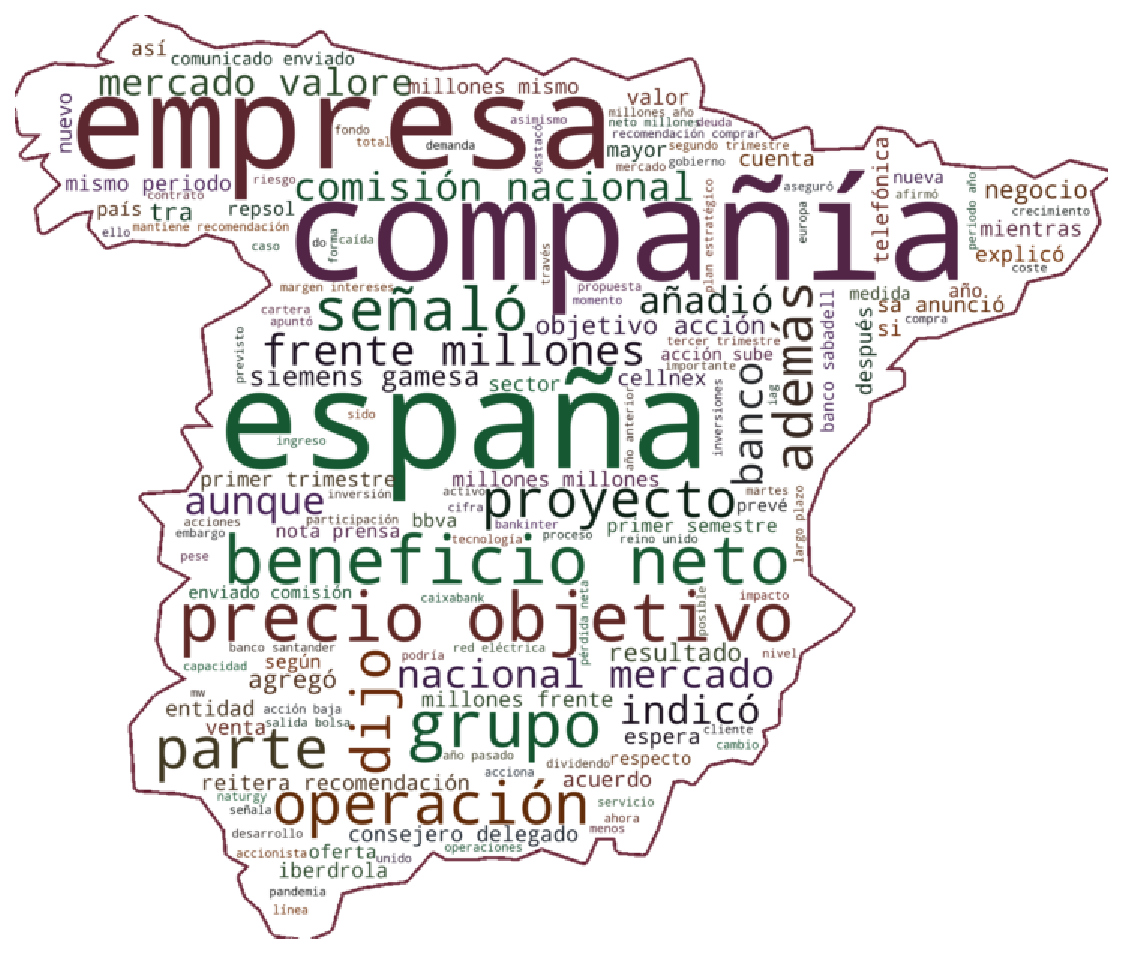
\includegraphics[scale=0.496]{fig_1_EDA_WordCloud.pdf}
  \label{fig:WordCloud}
  \subcaption*{\textit{Note: This Word Cloud visualizes the most frequent words in our dataset of Spanish business news articles. Larger words correspond to higher frequencies. The color of the words is purely for visual differentiation and holds no additional meaning. The most prominent words include \qquote{empresa} (firm), \qquote{compa��a} (company), and \qquote{espa�a} (Spain), reinforcing that the dataset primarily comprises Spanish business news, with a prevalence of technical terms such as \qquote{beneficio neto} (net profit), \qquote{precio objetivo} (target price), \qquote{proyecto} (project), and \qquote{operaci�n} (operation).}}
\end{figure}
%----------------------------------------------------

The distribution of the number of articles published per day is illustrated in \cref{fig:hist_1}, showing that the most frequent publication rate is between 5 and 10 articles per day, though some days exhibit unusually high publication counts. \cref{fig:hist_2} shows the distribution of the number of words per article, with the majority of articles containing between 70 and 280 words. This indicates that the articles are relatively succinct, providing direct information. 
However, the long right tail points to instances of more comprehensive coverage.

%----------------------------------------------------
\inserthere{fig:histograms}
\begin{figure}[H]
  \caption{Histogram of \# News Articles per Day and \# Words per Article}
  \centering
  \begin{subfigure}[b]{0.46\textwidth}
    \centering
    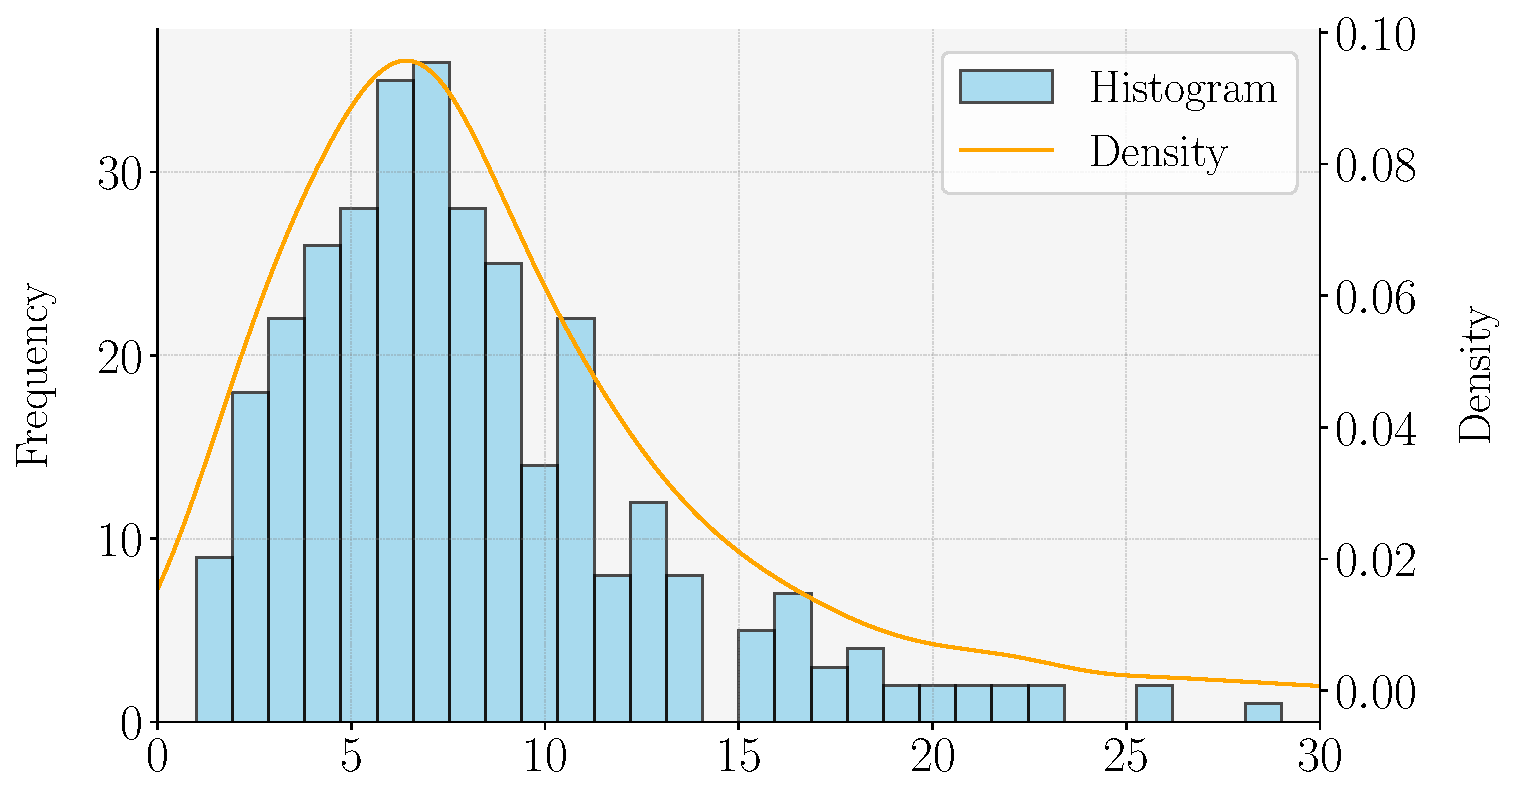
\includegraphics[width=\textwidth]{fig_2a_EDA_News_Articles_per_day.pdf}
    \caption{Number of News Articles per Day}
    \label{fig:hist_1}
  \end{subfigure}
  \hspace{0.05\textwidth} % Add horizontal space between the subfigures
  \begin{subfigure}[b]{0.46\textwidth}
    \centering
    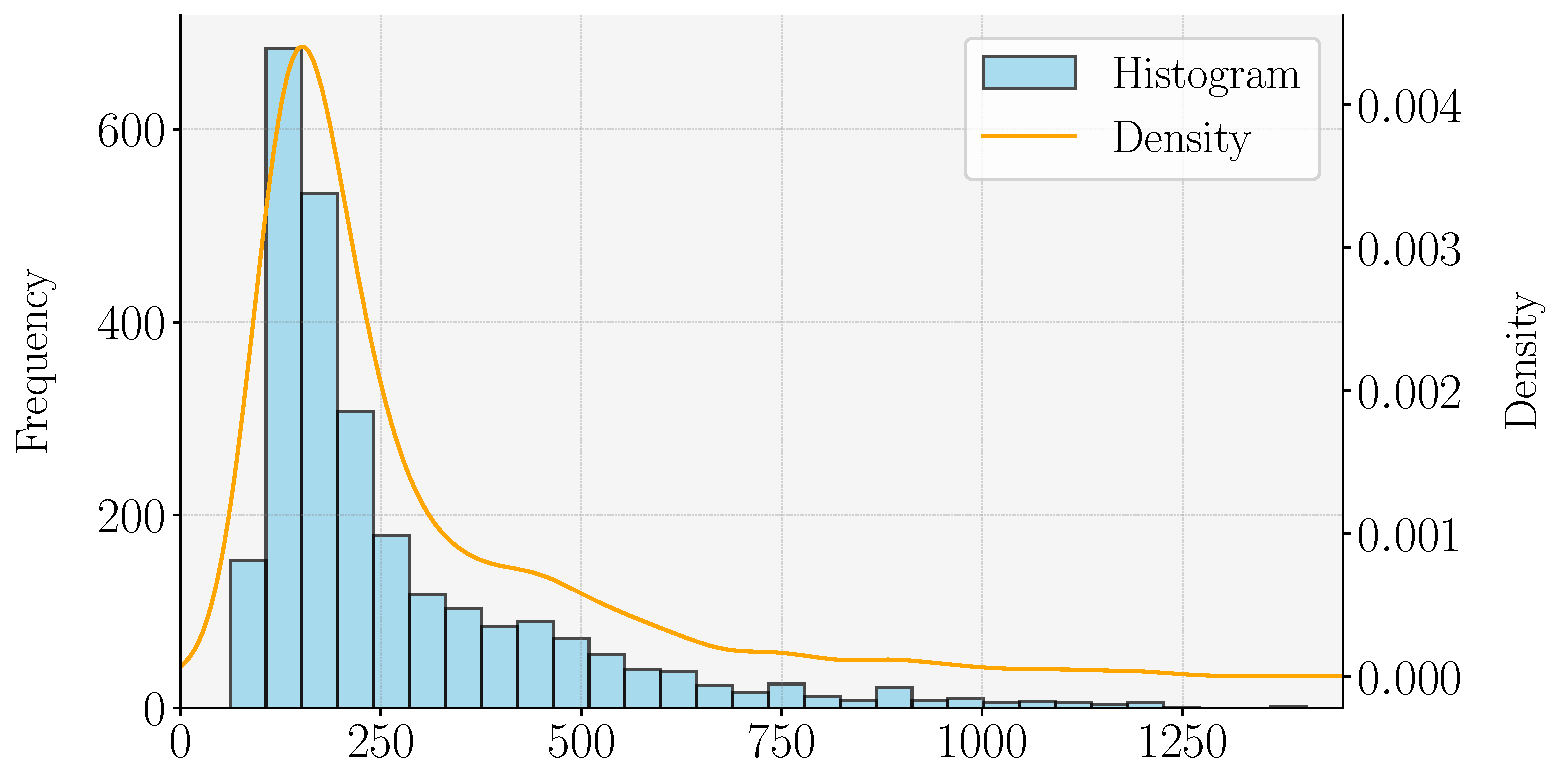
\includegraphics[width=\textwidth]{fig_2b_EDA_Words_per_Article.pdf}
    \caption{Number of Words per Article}
    \label{fig:hist_2}
  \end{subfigure}
  \label{fig:histograms}
  \subcaption*{\textit{Note: Panel (a) displays the distribution of the number of news articles published per day, with most days having between 5 and 10 articles. Panel (b) shows the distribution of the number of words per article, where the majority are between 70 and 280 words, suggesting concise reporting. However, the long right tail indicates instances of more comprehensive coverage.}}

\end{figure}
%----------------------------------------------------

The time series of the number of articles published per day throughout the sample period is shown in \Cref{fig:ts_articles}. The series exhibits considerable variability, with frequent fluctuations from fewer than 5 articles per day to sudden spikes exceeding 20 articles. The 30-day moving average smooths the series, confirming the previous observation that, on average, between 5 and 10 articles are published daily.

%----------------------------------------------------
\inserthere{fig:ts_articles}
\begin{figure}[H]
  \centering
  \caption{Time Series of Number of Articles per Day and 30-Period Moving Average}
  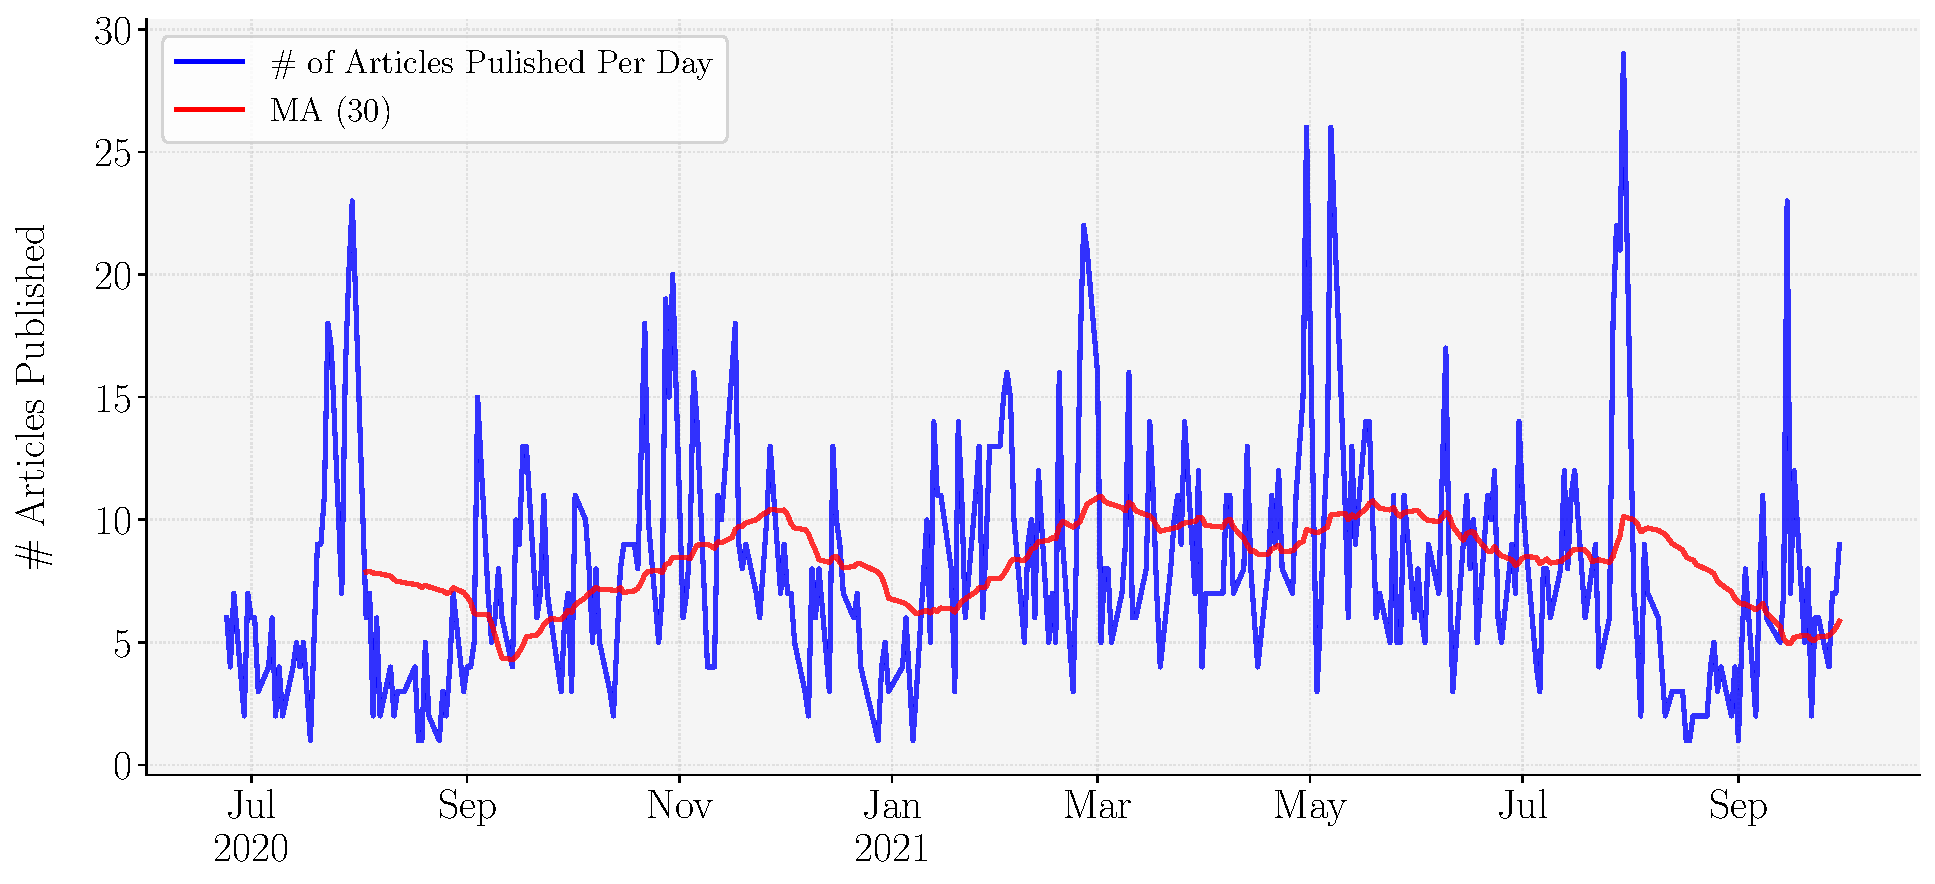
\includegraphics[scale=0.445]{fig_3_EDA_Time_Series_of_Articles.pdf}
  \label{fig:ts_articles}
  \subcaption*{\textit{Note: The time series shows the daily number of news articles published, characterized by significant variability with occasional sharp spikes. The 30-day moving average smooths these fluctuations, revealing an average publication rate of 5 to 10 articles per day.}}
\end{figure}
%----------------------------------------------------


\textbf{Data Availability.} 
% OPTION 1
The dataset used in this study contains confidential information provided under agreements with the Bank of Spain and Dow Jones Newswires, and cannot be shared publicly or with third parties. We are committed to transparency in our research methods and are available to discuss our methodology and provide additional non-confidential details upon request.
% OPTION 2
%Due to confidentiality and proprietary constraints, the dataset used in this research is not publicly available. Any inquiries regarding the data availability should be directed to the relevant parties who own the data.



%%%%%%%%%%%%%%%%% METHODOLOGY %%%%%%%%%%%%%%%%%%%%%%
\section{Mathematical Treatment of News Articles}

Our dataset consists of $N=2,613$ Spanish business news articles 
 sourced from DowJones and spanning the period from 2020/06/24 to 2021/09/30. 
 We denote as $\mathcal D$ the set of all articles in our sample.
 These articles have been specifically filtered to reference firms listed on the IBEX-35.
 Let $\F_{\t{IBEX35}}$ denote the universe of such firms. 
 Each article $i \in \mathcal{D}$ is a textual document detailing an event that directly pertains to a subset of firms $\mathcal{F}^i \subseteq \F_{\t{IBEX35}}$.
The publication date and time of each article are represented as $\mathcal{Y}_0^i = \langle d_0^i, t_0^i \rangle$, where $d_0^i$ captures the date 
(YYYY-MM-DD) 
and $t_0^i$ captures the time
 (HH:MM) 
 of publication. 
Therefore we observe the moment at which $\mathcal{F}^i$ receives the \qquote{treatment} of public news dissemination. 

\subsubsection*{Data Splitting}
For robust model development and evaluation, the dataset is partitioned into three sequential subsets: training, validation, and test:
$
\D := \D^{tr} \cup \D^{val} \cup \D^{test}.
$
Define $N_{split}:=|\D^{split}|$ for $split\in\3{tr,val,test}$, where $\abs{\cd}$ denotes the cardinality of a set. 
%
The training and validation sets collectively comprise 80\% of the total dataset $(\frac{N_{\text{tr}} + N_{\text{val}}}{N} = 0.8)$ and are instrumental in constructing and fine-tuning the trading strategy. The remaining 20\% $(\frac{N_{\text{test}}}{N} = 0.2)$ is reserved for out-of-sample testing to assess the performance and generalizability of the strategy under unseen conditions.
%----------------------------------------------------

%%%%%%%%%%%%%%%%%%%%%%%%%%%%%%%%%%%%%%%%%%%%%%%%%%%%%
%%%%%%%%%%%%%%%%%%%%%%%%%%%%%%%%%%%%%%%%%%%%%%%%%%%%%
\subsubsection*{Effective treatment day}
We are interested in examining the impact of each news article $i\in\D$ on the stock price of the firms that are affected directly (i.e.: all $j\in\F^i$). Since the publication datetime is not necessarily a trading datetime, we cannot directly gauge such an effect by looking at $\mathcal Y_0^i$. 
For this reason, we need to work through some definitions. 
Let $\T$ denote the set of all datetimes in the sample timeline and let $\widetilde{\T}\subset \T$ be the subset of Spanish trading datetimes associated to our sample.
\begin{align*}
\widetilde{\T} := 
\3{\angl{d,t} \mid d \in \tilde{\mathfrak d} ~\wedge~ t\in \tilde{\mathfrak t}}
,
\end{align*}
where 
$
\tilde{\mathfrak{d}}:=\{\tilde{\mathfrak{d}}_{[1]},\tilde{\mathfrak{d}}_{[2]}, \ldots \tilde{\mathfrak{d}}_{[n]}\}
$
is the ordered set of week and non-festive days according to the Spanish calendar in our data timeline,
and 
$\tilde{\mathfrak t}:=
\{t \mid \t{09:30} \leq t \leq  \t{17:30}\}
$
 are the Spanish stock market trading hours. 
Note that we use tildes to emphasize that we are considering trading dates or times. 

\bx 
Throughout our analysis, we will work with daily stock market closing data for each trading day. However, we will exploit the time component of $\mathcal Y_0^i$ to assign an \qquote{effective treatment date} to each article. Namely, define $\tilde d_0^i$ as the day at which article $i$'s information can be incorporated into the stock market; then, $\tilde d_0^i$ is the publication date if the article was published on a trading day before the stock market was closed, and is equal to the next closest trading day otherwise. 
To compute the next closest trading day to $d\in\mathfrak d$ within $\tilde{\mathfrak d}$, we need to work with a function $\Lambda:\mathfrak d \to \tilde{\mathfrak d}$ such that  
$\Lambda(d) 
:= 
\min \{ \tilde{d} \in \tilde{\mathfrak{d}} \mid \tilde{d} \geq d \}$. 
Thus, now we can define:
\begin{align*}
\tilde{d}_0^i :=
\mycases{llll}{
d_0^i & \IF & d_0^i \in \tilde{\mathfrak d} ~\wedge~t_0^i < \t{17:30}
\\
\Lambda(d_0^i)
& \IF & d_0^i \not \in \tilde{\mathfrak d} ~\vee~t_0^i \geq  \t{17:30}
}
.
\end{align*}


\section{Clustering News Articles}

In this section we present our clustering methodology based on news-implied firm-specific shock classifications and we compare it against a benchmark based on clustering the vector embedding representations of the articles. For ease of exposition, we will first present the benchmark model.

%----------------------------------------------------
\subsection{Benchmark: KMeans clustering of vector embeddings}

\subsubsection{Why this benchmark?}
In evaluating our novel Large Language Model (LLM) methodology for classifying news-implied firm-specific shocks, we selected KMeans clustering of high-dimensional vector embeddings as the benchmark over alternatives like sentiment analysis and topic modeling. Sentiment analysis, while straightforward, lacks the necessary granularity, offering only positive, negative, or neutral classifications, which is insufficient to compare with our granular LLM-based economic shock classification. Additionally, sentiment analysis focuses on the emotional tone rather than the economic impact, it is prone to inconsistencies due to linguistic nuances and it can deliver very different outcomes depending on the specific sentiment analysis tool employed.  

On the other hand, topic modeling provides more detailed classifications than sentiment analysis but relies on bag-of-words representations that fail to capture complex semantic relationships and contextual nuances essential for identifying economic shocks accurately. Vector embeddings, particularly those generated by transformer-based models, offer enhanced semantic representation by capturing context-dependent meanings and scaling efficiently with large datasets, making them more flexible and adaptable for clustering and classification. Although embeddings lack inherent interpretability, this issue is addressed by clustering, which allows us to infer meaningful firm-specific or industry-specific patterns from the grouped articles. 

Lastly, using embeddings as a benchmark is particularly compelling because they represent the foundational layer of an LLM. Namely, the first step in an LLM's processing pipeline is to transform the text that it is fed into embeddings for further processing. By benchmarking against embeddings, we ensure a direct and relevant comparison between the foundational representations used by LLMs and our specialized classification methodology. This comparison highlights the added value of the LLM's capacity to convert these semantic representations (i.e: the vector embeddings) into economically meaningful classifications. (i.e: our news-implied firm-specific shock classifications). Consequently, KMeans clustering of vector embeddings provides a robust, scalable, and economically pertinent benchmark, superior to sentiment analysis and topic modeling, for assessing our LLM-based classification of news-implied firm-specific shocks. A more detailed discussion can be found in \ref{sec:A7}. 


\subsubsection{Vector embeddings: \qquote{Transforming text into high-dimensional vectors}}


Any piece of text can be represented as a high-dimensional vector embedding by using a transformer. Transformers are a type of deep learning architecture introduced by 
\cite{vaswani2017attention} Vaswani et al. (2017) 
which have revolutionized natural language processing (\texttt{NLP}). The core idea behind them is the self-attention mechanism, which allows the model to weigh the importance of different words in a sentence when generating a representation for each word. This mechanism enables transformers to capture long-range dependencies and contextual relationships within the text more effectively than previous models like recurrent neural networks (\texttt{RNN}s).

\mx
A transformer model consists of an encoder (and potentially, a decoder as well) composed of multiple layers of self-attention and feedforward neural networks. In our context, we primarily use the encoder to convert a piece of text into a fixed-size vector, known as an embedding. 
Since our articles are written in Spanish, we employ a \texttt{Multilingual Sentence Transformer}, which has been trained on text from multiple languages. 
%

\mx 
For every news article $i\in\D$, we obtain a representative vector embedding $\mathbf{e}^i \in \mathbb{R}^{512}$ that provides a numerical representation of 
%
various aspects of the text, such as syntactic structure, semantic content, and contextual nuances.
%
While it is challenging to assign a specific human-readable meaning to each of the 512 components, we can interpret the vector as a whole in various ways:


\begin{itemize}
  \item \textit{Semantic Similarity}: Similar articles will have similar embeddings. For instance, if one article discusses a company's quarterly earnings and another article discusses the same company's annual earnings, their embeddings will be close in the 512-dimensional space.
  \item \textit{Topic Clustering}: Articles on similar topics will cluster together. For example, articles about financial markets might cluster in one region of the embedding space, while articles about mergers and acquisitions cluster in another.
  \item \textit{Sentiment Analysis}: Different regions of the embedding space can implicitly represent different sentiments. Articles with positive news might cluster in one area, while those with negative news cluster in another.

\end{itemize}

\subsubsection{Clustering embeddings with KMeans}


With the numerical representation of each article in the form of embeddings $\{\mbf e^i\}_{i\in\D}$, we now seek to identify groups of similar articles. 
%
Namely, we use the KMeans algorithm, a popular clustering method that assigns a set of vectors into $k$ clusters
$\mathcal G_{\t{KMeans}}:=\{0,1,...,k-1\}$ to minimize the within-cluster sum of squares (WCSS). 
The implementation of this clustering algorithm is methodically presented in Appendix \cref{alg:KMeans}
Each cluster $g\in\mathcal G_{\t{KMeans}}$ defines a centroid $\mbf c_g$, which is the average vector of all the members of a cluster.
%
In the first step, we apply the algorithm to the training data ($\D^{tr}$).
$$
\begin{array}{rllll}
\underset{\{\mathcal{D}_g^{tr}\},\{\mbf c_g\}}{\min}
&  \sum_{g=1}^k \sum_{i \in \mathcal{D}_g^{tr}} \|\mathbf{e}^i-\mbf c_g \|_{2}^2
\\[0.8em]
\t{s.t.} 
&
$$\begin{array}{|ll}
\bigcup_{g=1}^k \mathcal{D}_g^{tr} = \D^{tr}
\\[0.7em]
\mathcal{D}_g^{tr} \cap \mathcal{D}_h^{tr}=\emptyset ~~~~\forall g,h\in \mathcal G_{\t{KMeans}}:g \neq h
\end{array}$$
\end{array}
~~.
$$

The optimal number of clusters $k^*$ in this algorithm is to be set exogenously. Here, we take it to maximize the average silhouette score in the training sample over some grid $\mbf k$ of cluster sizes $k$:
$$
k^* := \arg \max_{k\in \mbf k}\frac{1}{|\D^{tr}|} \sum_{i\in\D^{tr}} 
s_k(\mbf e^i)
~.
$$
The silhouette score $s_k(\mbf e^i)\in \2{-1,1}$ measures how well an embedding is clustered by comparing its similarity to its own cluster (\textit{intra-cluster distance}) with its similarity to the nearest other cluster (\textit{inter-cluster distance}). A clustering configuration with a higher average silhouette score (close to +1) is considered better because it indicates that clusters are dense and well-separated. Formally, the silhouette score is defined as
\begin{align*}
s_k(\mbf e^i):=
\frac{b_k\left(\mathbf{e}^i\right)-a_k\left(\mathbf{e}^i\right)}
{\max \3{a_k\left(\mathbf{e}^i\right), b_k\left(\mathbf{e}^i\right)}}
~,
\end{align*}
where, for $i\in \D_g^{tr}$, the \textit{intra-cluster distance} is defined as 
$
a_k (\mathbf{e}^i)
:=
%\frac{1}{|\D^{tr}_g|-1} 
(|\D^{tr}_g|-1)^{-1}
\sum_{m \in \D_g^{tr}, m \neq i} 
\|
\mathbf{e}^i-\mathbf{e}^m 
\|_{2}
~
$
and it represents the average distance from an embedding $\mathbf{e}^i$ to all other embeddings in the same cluster, while the \textit{inter-cluster distance} is
$
b_k(\mathbf{e}^i)
:=\min _{l \neq g} 
%\frac{1}{|\D^{tr}_l|}
(|\D^{tr}_l|)^{-1}
\sum_{m \in \D_l^{tr}}
\|
\mathbf{e}^i-\mathbf{e}^m
\|_{2}
$
and it represents the minimum average distance from an embedding $\mathbf{e}^i$ to all embeddings in the nearest different cluster. 

In \cref{fig:silhouette_score} we plot the average silhouette score for $\D^{tr}$ computed over a grid $\mbf k$ ranging from 2 to 100. The vertical dashed green line signals the maximizer of the grid, which corresponds to a cluster size of $k^*=26$. 

%----------------------------------------------------
\inserthere{fig:silhouette_score}
\begin{figure}[H]
  \centering
\caption{Average Silhouette Scores in the Training data}
  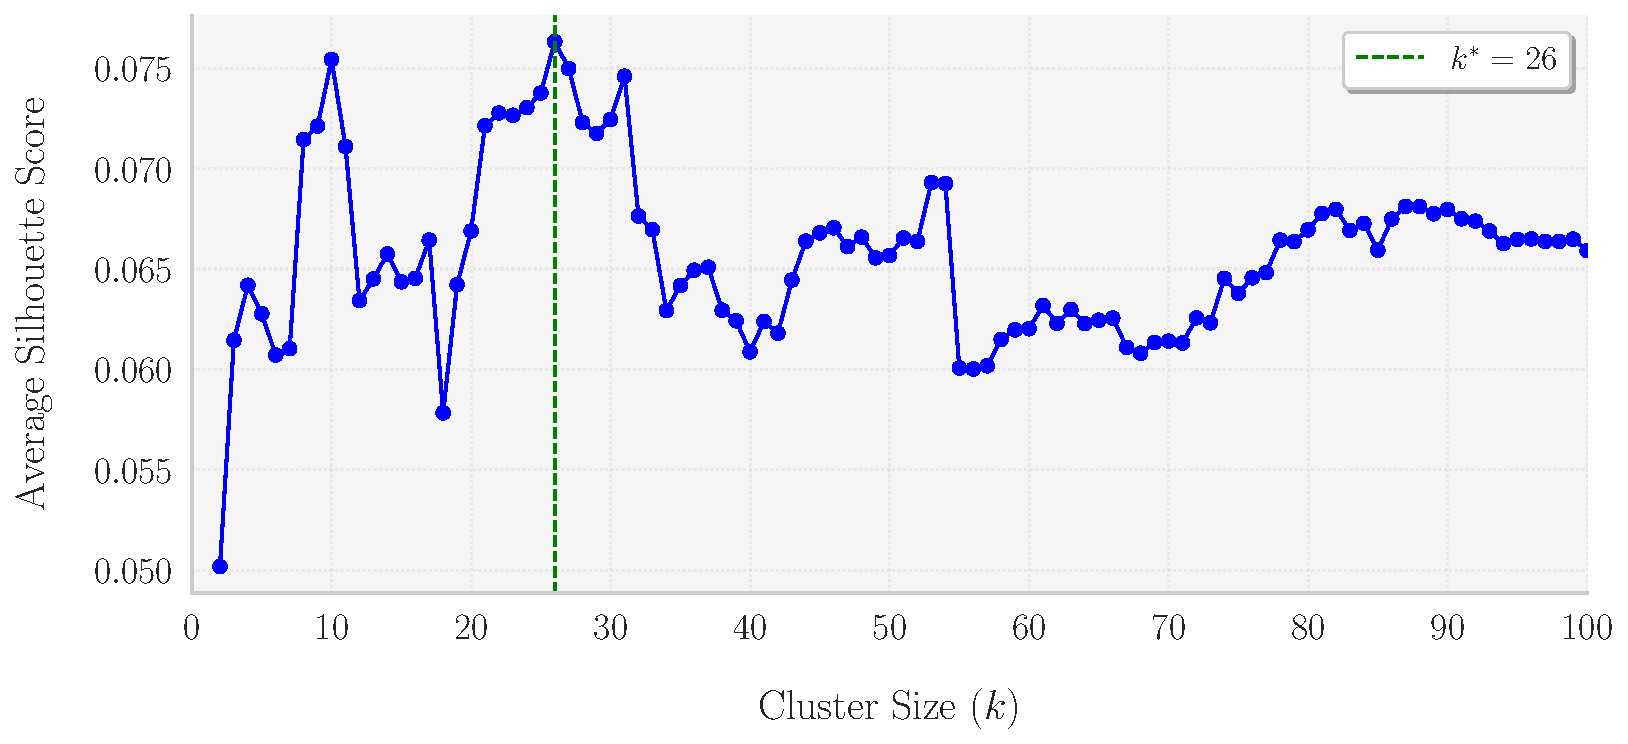
\includegraphics[scale=0.5]{fig_4_KMeans_Clustering_Silhouette_Score.pdf}
\subcaption*{\textit{Note: The plot presents the average silhouette scores calculated on the training data $\D^{tr}$ for various cluster sizes $k$ ranging from 2 to 100. The silhouette score measures how well data points fit within their assigned cluster by comparing intra-cluster cohesion with inter-cluster separation. A higher silhouette score (closer to +1) indicates better-defined clusters. The optimal number of clusters, $k^*=26$, which maximizes the average silhouette score, is marked by a vertical dashed green line.}}
\label{fig:silhouette_score}
\end{figure}
%----------------------------------------------------




\mx
Given the optimal number of clusters $k^*$, we fit the KMeans algorithm on the training embeddings 
$\{\mbf e^i \mid i\in\D^{tr}\}$
%$\{ \mathbf{e}^1, \mathbf{e}^2, \ldots, \mathbf{e}^{N_{tr}} \}$
 to obtain the centroids $\{ \mathbf{c}^{tr}_1, \mathbf{c}^{tr}_2, \ldots, \mathbf{c}^{tr}_{k^*} \}$. Following \cref{alg:KMeans} (detailed in \ref{sec:A1}):
$$
\{ \mathbf{c}^{tr}_1, \mathbf{c}^{tr}_2, \ldots, \mathbf{c}^{tr}_{k^*} \} = \text{KMeans} ( \{ \mathbf{e}^1, \mathbf{e}^2, \ldots, \mathbf{e}^{N_{tr}} \}, k^* )
~.
$$

We then find the cluster associated to each embedding $\mathbf{e}^i$ in the validation set 
$\{\mbf e^i \mid i\in\D^{val}\}$ according to the centroids resulting from clustering the training data $\{\mbf c_1^{tr},..., \mbf c_{k^*}^{tr}\}$.
This allows us to obtain the clustering of the news articles in the validation sample
$$
\D_g^{val} = 
\3{ 
i\in \D^{val} 
\c g = \arg \min_{\ell\in\G} \|\mathbf{e}^i - \mathbf{c}^{tr}_{\ell}\|_{2}^2
}
\quad 
\forall g\in\G_{\t{KMeans}}
.
$$

Similarly, by assigning each embedding $\mathbf{e}^i\in \{\mbf e^i \mid i\in\D^{test}\}$
 to the nearest centroid $\mathbf{c}^{tr}_g$, we obtain the clusters in the test set
$$
\D_g^{test} = 
\3{ 
i\in \D^{test}
\c g = \arg \min_{\ell\in\G} \|\mathbf{e}^i - \mathbf{c}^{tr}_{\ell}\|_{2}^2 
}
\quad 
\forall g\in\G_{\t{KMeans}}
.
$$
%----------------------------------------------------

%----------------------------------------------------
\inserthere{fig:combined_plots}
\begin{figure}[H]
    \centering
    \caption{Distribution of articles through KMeans clusters}
    
    % Upper plot
    \begin{subfigure}[b]{\textwidth}
        \caption{All data ($\mathcal D$)}
        \centering
        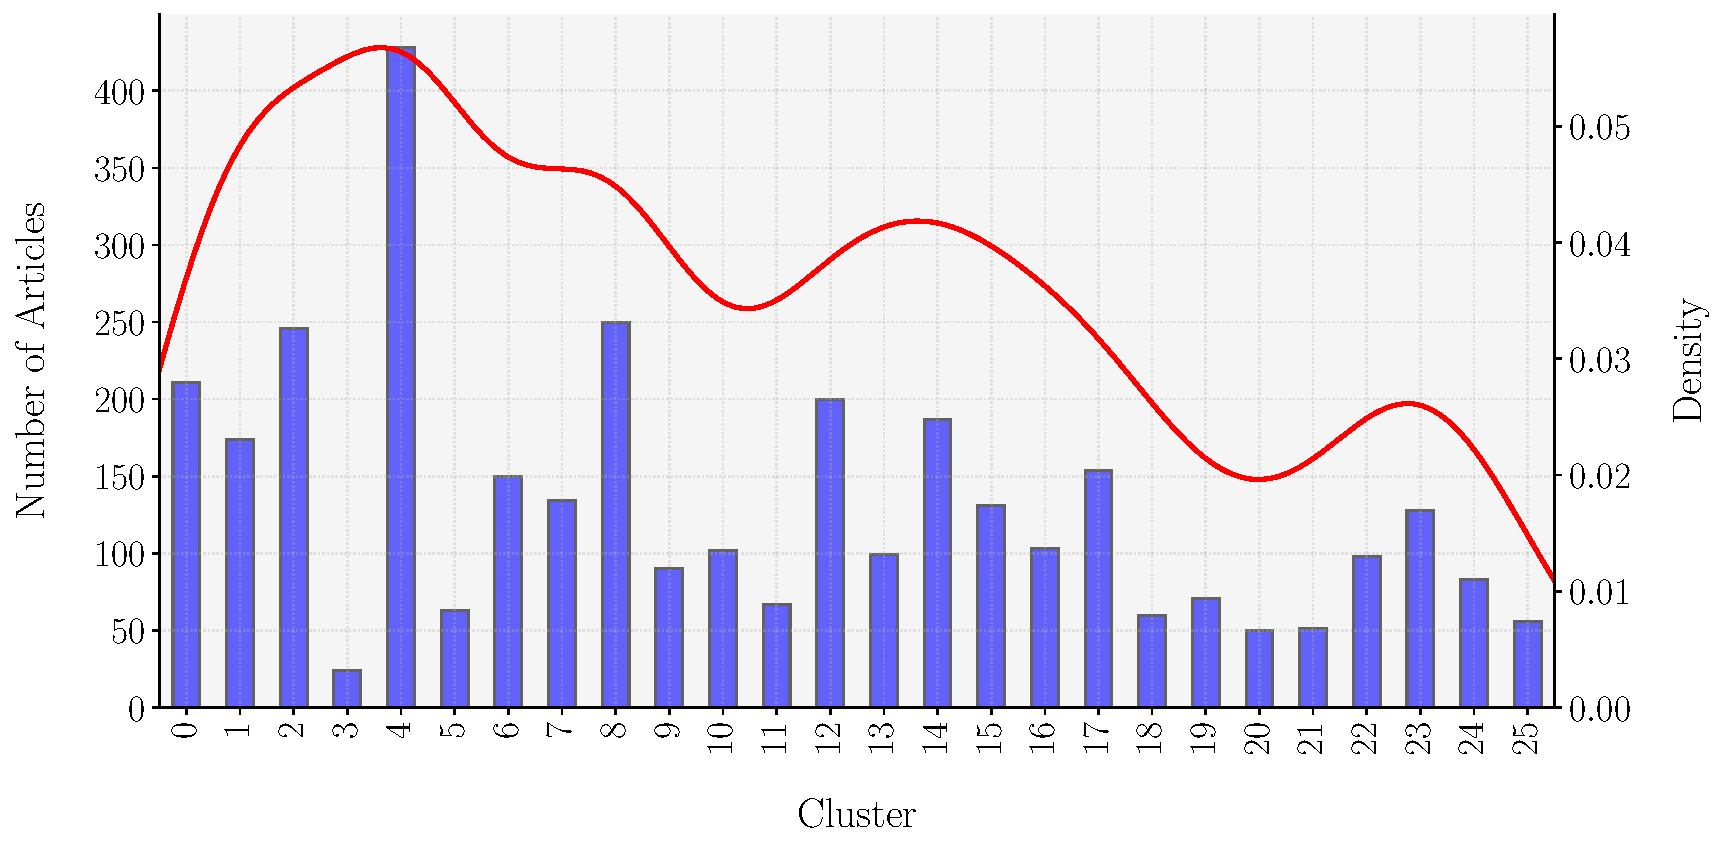
\includegraphics[scale=0.45]{fig_5a_KMeans_Cluster_Distribution.pdf}
        \label{fig:all_data}
    \end{subfigure}

    % Lower plots
    \begin{subfigure}[b]{0.32\textwidth}
        \caption{Training data ($\D^{tr}$)}
        \centering
        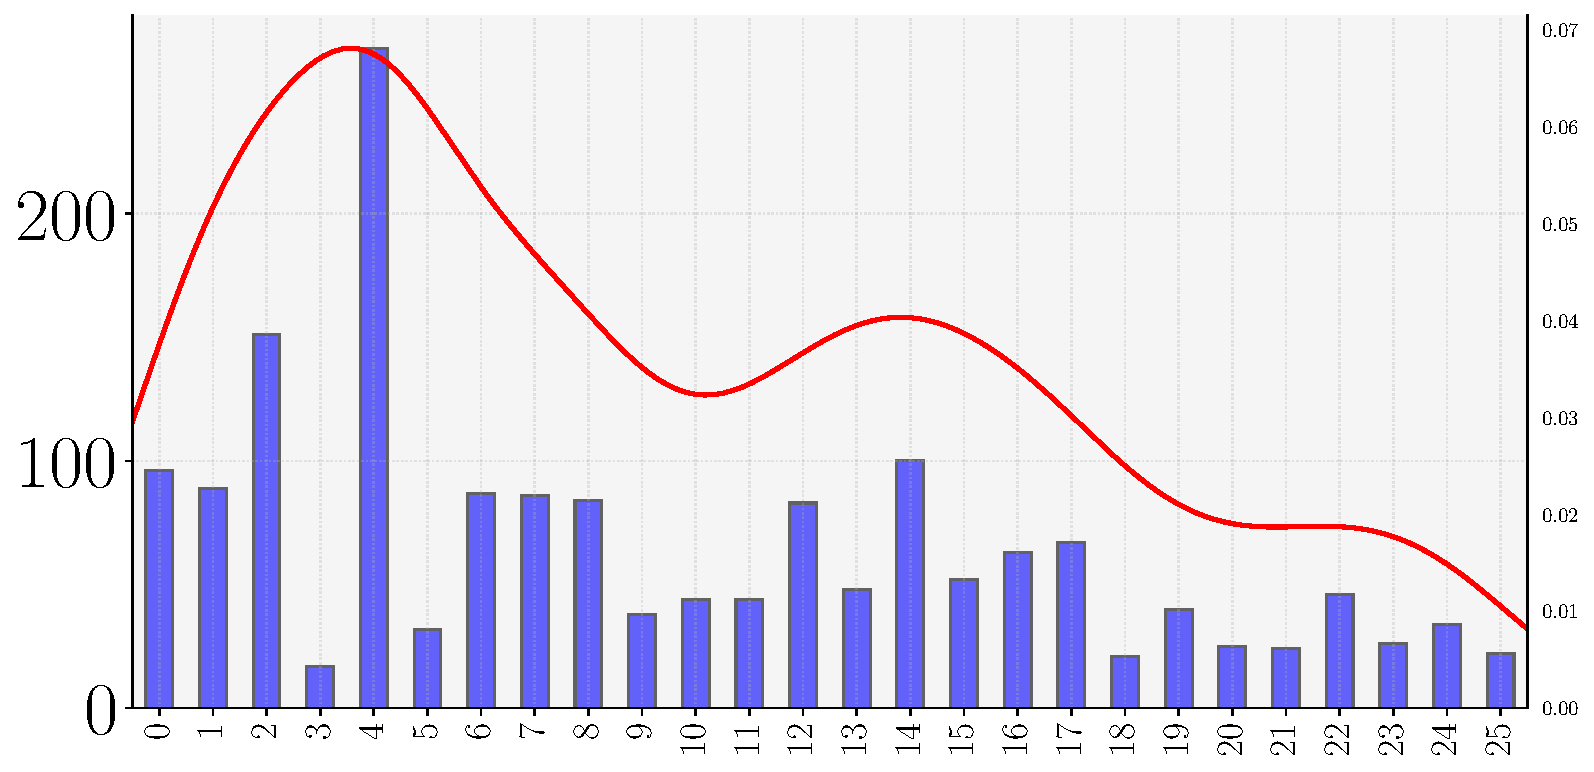
\includegraphics[width=\textwidth]{fig_5b_KMeans_Cluster_Distribution_Train.pdf}
        \label{fig:train_data}
    \end{subfigure}
    \begin{subfigure}[b]{0.32\textwidth}
        \caption{Validation data ($\D^{val}$)}
        \centering
        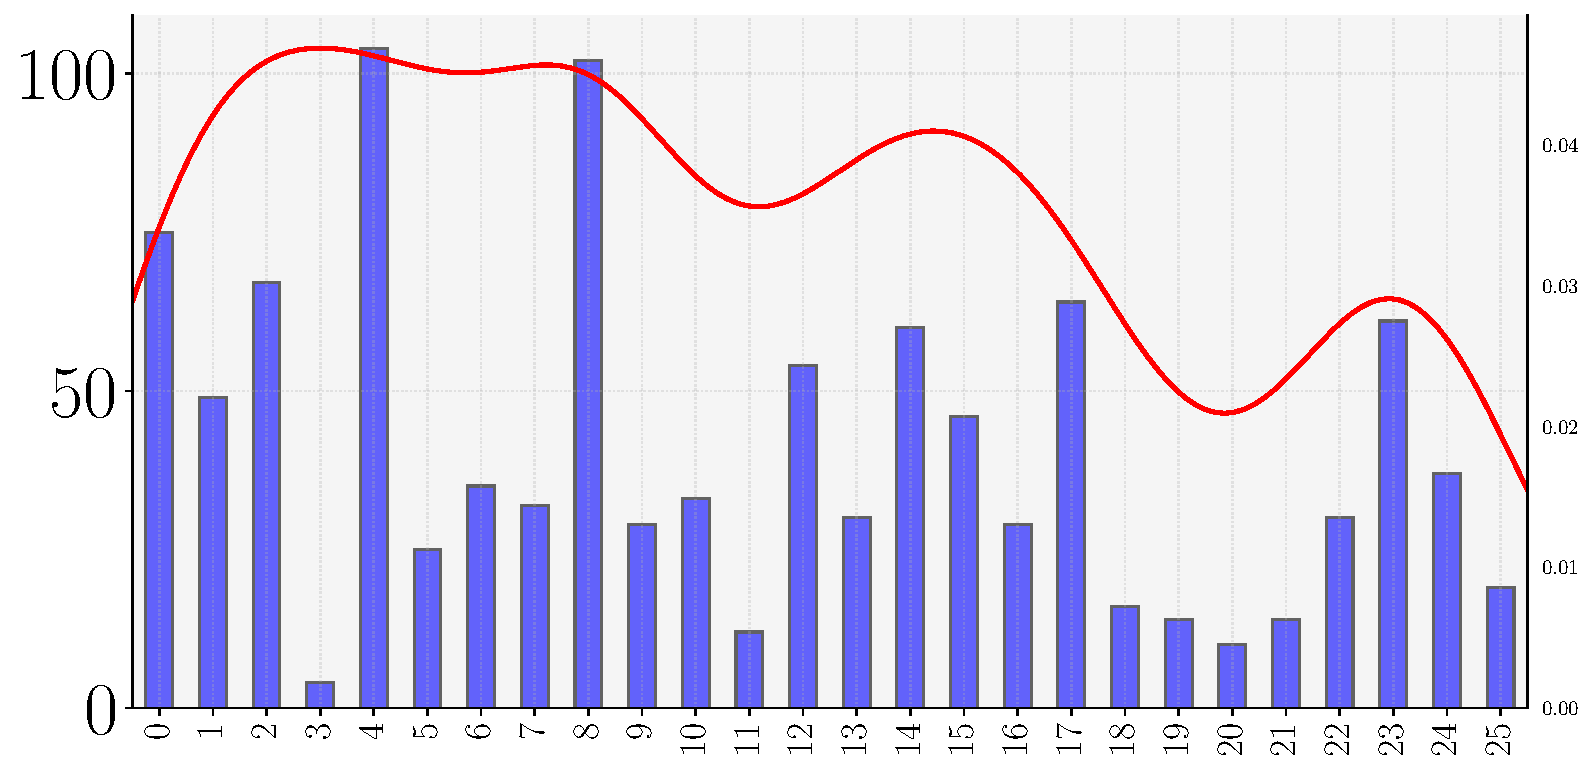
\includegraphics[width=\textwidth]{fig_5c_KMeans_Cluster_Distribution_Validation.pdf}
        \label{fig:val_data}
    \end{subfigure}
    \begin{subfigure}[b]{0.32\textwidth}
        \caption{Test data ($\D^{test}$)}
        \centering
        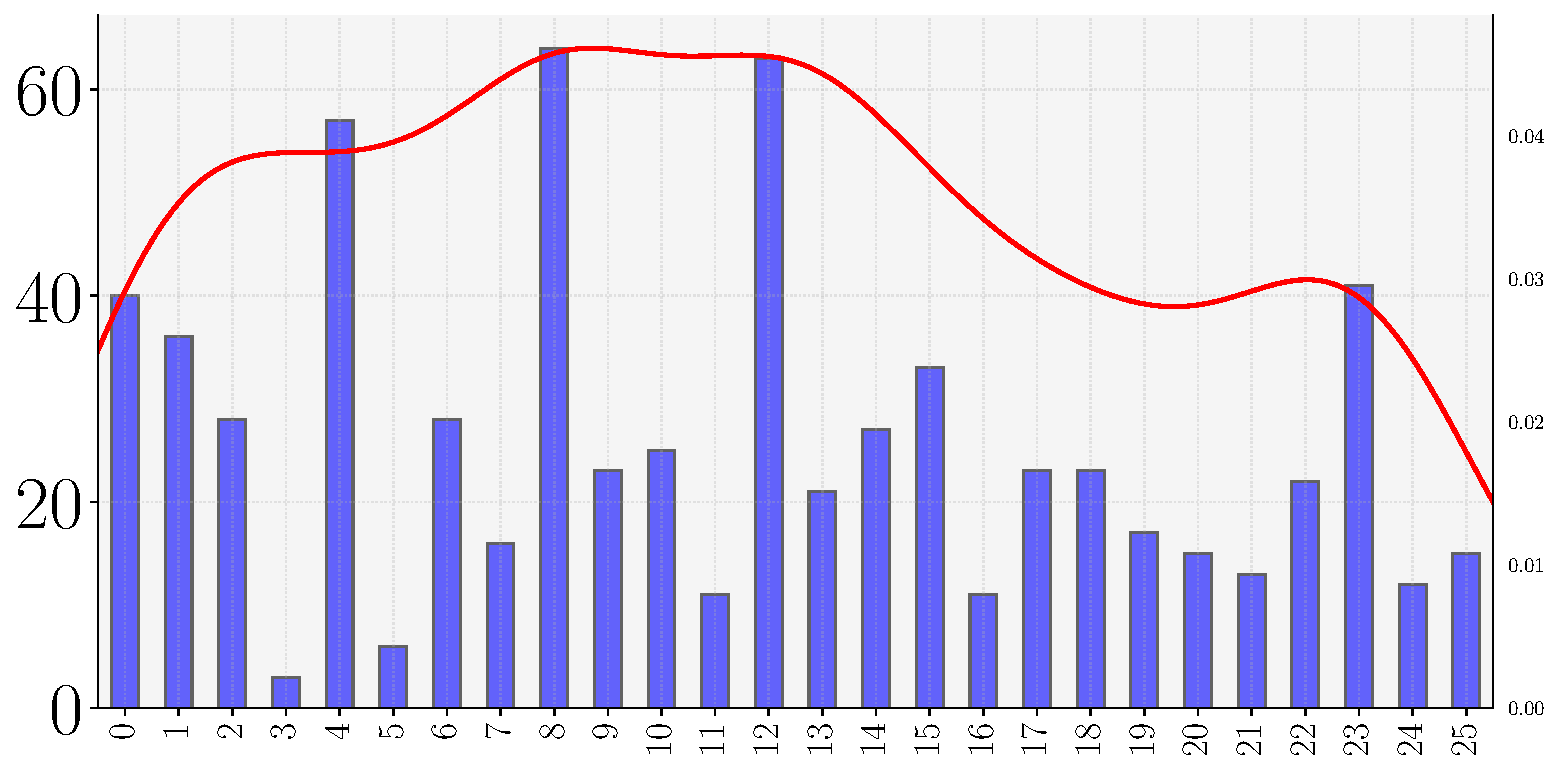
\includegraphics[width=\textwidth]{fig_5d_KMeans_Cluster_Distribution_Test.pdf}
        \label{fig:test_data}
    \end{subfigure}
    \label{fig:combined_plots}
\subcaption*{\textit{Note: This figure presents the distribution of articles across the $k^*=26$ clusters, where the centroids were determined by applying the KMeans algorithm to the article embeddings from the training data. Panel \textsc{(a)} shows the distribution for the entire dataset ($\mathcal{D}$), while Panels \textsc{(b)}, \textsc{(c)}, and \textsc{(d)} illustrate the distributions for the training ($\mathcal{D}^{tr}$), validation ($\mathcal{D}^{val}$), and test ($\mathcal{D}^{test}$) datasets, respectively. The differences in distribution across splits suggest some temporal instability in the clustering results.}}
\end{figure}
%----------------------------------------------------

In \cref{fig:combined_plots} we can see that the distribution of articles in the whole sample ($\D$) is fairly homogenous across the 26 clusters, with each cluster containing between 50 and 250 articles on average. The notable exceptions are cluster 3, which contains only 24 articles, and cluster 4, which concentrates 428 articles. However, the distribution profile is not consistent over data splits, which indicates that this classification procedure is unstable over time.

\mx 
Although not directly interpretable, by looking at the articles pooled in a certain cluster, we can provide some intuition of what it represents. In most cases, each cluster contains articles involving a firm or set of firms in the same sector. For example, cluster 3 pools articles about Telef�nica and Cellnex (telecoms), cluster 4 contains articles about CaixaBank, cluster 9 concentrates articles about Repsol, cluster 12 about Iberdrola, cluster 15 gathers articles on Infrastructure (led by ACS and Acciona) and so on.

\mx 
However, there are some exceptions to this general rule, for example, cluster 0 is a \qquote{miscellanous} cluster:
% with no clear pattern: 
 it covers articles about different firms with no apparent relation between them. Another example is cluster 1, which pools articles related to the quarterly or semiannual publication of results by different firms. In Appendix \cref{tab:KMeans_Articles_3_English} we provide a sample of 3 articles for each cluster and propose a name for each one based on the articles they pool.

%----------------------------------------------------

%----------------------------------------------------
\subsection{LLM-based approach: \qquote{What if an LLM reads the news?}}

One may wonder whether empowering an LLM to parse news articles according to a predefined schema that guides it in ellucidating news-implied firm-specific shocks can deliver better insights on how markets react to new information. In this section we will briefly introduce what Large Language Models are, how they have evolved and then, we will dive into how we can guide them to produce an economically structured analysis of business news. 

%%%%%%%%%%%%%%%%%%%%%%%%%%%%%%%%%%%%%%%%%%%%%%%%%%%%%
%%%%%%%%%%%%%%%%%%%%%%%%%%%%%%%%%%%%%%%%%%%%%%%%%%%%%
\subsubsection{Large Language Models}

In natural language processing (NLP), Large Language Models (LLMs) are designed to \qquote{understand} and generate human-like text. These models utilize the transformer architecture, which excels in modeling complex language tasks by capturing long-range dependencies and contextual relationships.

\mx 
At the heart of LLMs lies the concept of tokens, which serve as the elemental units of text. Tokens can be individual words, subword units, or characters. Let $x_{1:n}:=\3{x_1, x_2, \ldots, x_n}$ represent a sequence of tokens. The goal of an LLM is to estimate the probability distribution of the next token $x_{n+1}$ conditioned on the previous tokens $x_{1:n}$
$$
\P\2{x_{n+1} \mid \3{x_1, x_2, \ldots, x_n}}
.
$$

%\mx 
An LLM is a neural network architecture designed to learn and approximate this conditional probability distribution over sequences of tokens with a large number of parameters $\Theta$. Namely, we can formulate an LLM as a parameterized function $f_{\Theta}$ that maps a sequence of tokens $\3{x_1, x_2, \ldots, x_n}$ to a probability distribution over the vocabulary, where the parameters $\Theta$ are learned from a large corpus of text training data.
$$
f_{\Theta}:\3{x_1, x_2, \ldots, x_n} \rightarrow 
\P\2{x_{n+1} \mid \3{x_1, x_2, \ldots, x_n} ; \Theta}
$$

%\mx 
Interacting with an LLM involves specifying a prefix sequence $x_{1:n}$, termed the \qquote{prompt}, and sampling the subsequent tokens $x_{n+1:z}$, known as the \qquote{completion}. This process enables users to guide and control the generation of text according to desired contexts and constraints.
$$
\ub{\3{x_1,\ldots,x_n}}{\t{prompt}} \longrightarrow \ub{\3{x_{n+1},\ldots,x_z}}{\t{completion}}
$$


\subsubsection{Evolution of LLMs}
The transformer architecture, introduced in the seminal work ``\textit{Attention Is All You Need}'' 
(\cite{vaswani2017attention} Vaswani et al., 2017), 
revolutionized LLM development due to its superior handling of long-range dependencies and efficient parallelization of computations.  Subsequent advancements include the encoder-only \texttt{BERT} model 
(\cite{devlin2018bert} Devlin et al., 2018), 
showcasing the power of pre-training on large datasets for fine-tuning on specific tasks. 

\mx 
Conversely, OpenAI's \texttt{GPT} series 
(\cite{radford2018improving} Radford et al., 2018) 
demonstrated the potential of decoder-only models for generative tasks. In particular, the release of \texttt{GPT-3} marked a significant leap in LLM capabilities with its 175 billion parameters and remarkable few-shot learning abilities. This model highlighted the importance of prompt engineering, where carefully crafted prompts can guide model outputs without extensive fine-tuning.  

\mx 
The trend towards open-source models like \texttt{BLOOM} 
(\cite{le2023bloom} Le Scao et al., 2023), \texttt{Mixtral} and Meta's \texttt{Llama} series 
(\citep{touvron2023llama} Touvron et al., 2023)
emphasizes accessibility and transparency in LLM development.  The latest models, including OpenAI's  \texttt{GPT-4o} and \texttt{GPT-o1}, Google's \texttt{Gemini} and \texttt{Mixtral} and \texttt{Gemma}, Anthropic's \texttt{Claude 3.5 Sonnet}, and Meta's \texttt{Llama-3} series
% \texttt{Llama-3}, \texttt{Llama-3.1} and  \texttt{Llama-3.2} 
continue to push boundaries with improved accuracy, multimodal capabilities, and larger context windows.

\subsubsection{Function Calling with Llama-3}

In our endeavor we will employ \texttt{Llama-3}, developed by Meta AI and released on April 18, 2024 %
%
\footnote{
\href{https://ai.meta.com/blog/meta-llama-3/}
{\qquote{Introducing Meta Llama 3: The most capable openly available LLM to date}
[April 18, 2024]}
}
%
. This model has been pre-trained on approximately 15 trillion tokens of text gathered from ``publicly available sources'' and it comes in two sizes: 8 billion and 70 billion parameters. In this application, we will employ the 70B version, which we will access through an API via \texttt{GroqCloud}.

\mx 
Moreover, we will employ a \textit{function calling} approach to streamline the process of interacting with the LLM. This implies prespecifying a set of functions to the LLM that will then be passed through our dataset of news articles to obtain a structured output in \texttt{JSON} format. The formal procedure is thoroughly described in Appendix \cref{alg:function_calling}

\mx 
Each article $i\in\D$ implies a conversation with the LLM. The structure of the conversation implies defining first a ``system message'', which provides a general context and purpose to the model. In our case:

\begin{quote}
\textit{$-$ You are a function calling LLM that analyses business news in Spanish.  \\
$-$ For every article, you must identify the firms directly affected by the news. Do not include every firm mentioned in the article, only include those that are directly affected by the shocks narrated therein. 
\\
$-$ The identified firms must be Spanish and should be publicly listed in the Spanish exchange (their ticker is of the form `TICKER.MC'). Do not include non-Spanish foreign firms. Do not include Spanish firms that are not publicly traded. \\
$-$ For each identified firm, classify the shocks that affect them (type, magnitude, category). The type of shock can be `demand', `supply', `financial', `policy', or `technology'. The magnitude can be `minor' or `major'. The direction can be `positive' or `negative'. \\
$-$ If a firm is affected neutrally by the news article, don't include it in the analysis.
}
\end{quote}

Then, a news article is fed to the LLM. For illustration purposes, we will work with Example \ref{news:article-cellnex-telefonica}:

%%%%%%%%%%%%%%% ENGLISH VERSION %%%%%%%%%%%%%%%%%%%
\begin{news}
[An article about Cellnex and Telef�nica (translated into English)]
[news:article-cellnex-telefonica]
{Cellnex will face more competition in Europe}
Telef�nica's (TEF.MC) subsidiary, Telxius Telecom, has agreed to sell its telecommunications tower division in Europe and Latin America to American Tower (AMT), which will expand the latter's presence in Europe and increase competition for the Spanish wireless telecommunications group Cellnex Telecom (CLNX.MC), according to Equita Sim. The transaction "represents the entry of a new independent tower operator into the Spanish market and potentially more competition for future growth in the European market as well," says the brokerage firm.		
\end{news}

Next, we define an umbrella function \qquote{firms}, which asks the LLM to identify the set $\F^i_{LLM}$ for each $i\in\D$. Then, for each $j\in\F_{LLM}^i$ we ask the LLM to categorize the type, expected magnitude, and expected direction that the shock described in the article implies in that particular firm $j$.
%----------------------------------------------------
\inserthere{tab:function_calling_structure}

\begin{table}[H]
\centering
\begin{threeparttable}
\caption{Function calling schema}
%{\footnotesize
%\renewcommand{\arraystretch}{1}
\begin{tabular}{lL{4.1cm}L{6.8cm}L{5cm}}
%%%%%%%%%%%%%%%%%%%%%%%%%%%%%%%%%%%%%%%%%%%%%%%%%%%%%
%%%%%%%%%%%%%%%%%%%%%%%%%%%%%%%%%%%%%%%%%%%%%%%%%%%%%
\hline \Xhline{2\arrayrulewidth}
%\rowcolor{gray!10}
\multicolumn{2}{l}{\textbf{Function}} & \textbf{Prompt} & \textbf{Options} \tabularnewline
\hline \Xhline{2\arrayrulewidth} 
\multicolumn{2}{l}{1. \texttt{firms}} & \qquote{List all the firms affected by the events narrated in the article} & \texttt{array} \tabularnewline
\hline
 & 1.1. \texttt{firm} & \qquote{Iterate over each \textnormal{\texttt{firm}} in \textnormal{\texttt{firms}}} & \texttt{string}
 \tabularnewline
\cline{2-4} \cline{3-4} \cline{4-4} 
 & 1.2. \texttt{ticker} & \qquote{State the stock market ticker of \textnormal{\texttt{firm}} } & \texttt{string}
 \tabularnewline
\cline{2-4} \cline{3-4} \cline{4-4} 
 & 1.3. \texttt{shock\_type} & \qquote{What type of shock does this article imply on \textnormal{\texttt{firm}} ?} & \{demand, supply, financial, \newline technology, policy\}\tabularnewline
\cline{2-4} \cline{3-4} \cline{4-4} 
 & 1.4. \texttt{shock\_magnitude} & \qquote{How much impact is this shock expected to have on \textnormal{\texttt{firm}}?} & \{minor, major\}\tabularnewline
\cline{2-4} \cline{3-4} \cline{4-4} 
 & 1.5. \texttt{shock\_direction} & \qquote{In what direction is this shock expected to impact \textnormal{\texttt{firm}}?} & \{positive, negative\}\tabularnewline 
%\cline{2-4} \cline{3-4} \cline{4-4} 
\hline \Xhline{2\arrayrulewidth}
\end{tabular}
%}
%\begin{tablenotes}
%\footnotesize
%\mx
%\item \textit{Note: 
%For clarity of exposition, the actual prompts passed to LlaMA are avoided here but can be found in the code. 
%The ``Options'' column imposes the asnwer format that the LLM must follow. For example, in \texttt{firms}, the option \texttt{array} indicates that the answer must be an enumeration of firms, while the option \texttt{string} in the subfunctions \texttt{firm} and \texttt{ticker} indicates that the answer must be a single name. Finally, the \texttt{shock\_} subfunctions ask the LLM to choose from a predefined set of options.
%}
%\end{tablenotes}
\label{tab:function_calling_structure}
\end{threeparttable}
\mx 
\subcaption*{\textit{
This table outlines the structure of the function calling schema we designed to guide the LLM through the analysis of news-implied firm-specific economic shocks. The \qquote{Function} column specifices the name of the tool passed to the LLM. We can understand the umbrella function \texttt{firms} as running a loop over each of its arguments, with the indented subfunctions being referred to the specific argument passed to them. The \qquote{Prompt} column provides an example of the simplified instructions given to the LLM (the actual prompts are longer as the LLM needs clear and detailed instructions, with useful examples for context).  Finally, the ``Options'' column imposes the answer format that the LLM must follow. For example, in \texttt{firms}, the ``\texttt{array}'' option indicates that the answer must be an enumeration of firms, while the  ``\texttt{string}'' option in the subfunctions \texttt{firm} and \texttt{ticker} indicates that the answer must be a single string. Finally, the \texttt{shock\_} subfunctions ask the LLM to choose from a predefined set of possible responses.
}}
\end{table}



%%%%%%%%%%%%%%%%%%%%%%%%%%%%%%%%%%%%%%%%%%%%%%%%%%%%%
%%%%%%%%%%%%%%%%%%%%%%%%%%%%%%%%%%%%%%%%%%%%%%%%%%%%%

%\begin{table}[H]
%\centering
%\begin{threeparttable}
%\caption{Function calling schema}
%{\small
%\begin{tabular}{l||L{4.1cm}|L{6.8cm}|L{5cm}|}
%%%%%%%%%%%%%%%%%%%%%%%%%%%%%%%%%%%%%%%%%%%%%%%%%%%%%%
%%%%%%%%%%%%%%%%%%%%%%%%%%%%%%%%%%%%%%%%%%%%%%%%%%%%%%
%\hline 
%\multicolumn{2}{|l|}{Function} & Description & Options \tabularnewline
%\hline 
%\hline 
%%\multicolumn{2}{|l|}{1. \texttt{publication\_time}} & Date and time of publication & ``''\tabularnewline
%%\hline 
%%\multicolumn{2}{|l|}{2. \texttt{scope}} & Scope or focus of the news article's impact. & \{Firm, Industry, Economy\}\tabularnewline
%%\hline 
%%\multicolumn{2}{|l|}{3. \texttt{news\_category}} & Type of information provided in the article & \{New, Historical, \newline Analysis/Comments\}\tabularnewline
%%\hline 
%\multicolumn{2}{|l|}{1. \texttt{firms}} & List all the firms affected by the events narrated in the article & \texttt{array} \tabularnewline
%\hline
% & 1.1. \texttt{firm} & Iterate over each firm in \texttt{firms} & \texttt{string}
% \tabularnewline
%\cline{2-4} \cline{3-4} \cline{4-4} 
% & 1.2. \texttt{ticker} & State the stock market ticker of this firm & \texttt{string}
% \tabularnewline
%\cline{2-4} \cline{3-4} \cline{4-4} 
% & 1.3. \texttt{shock\_type} & What type of shock does the article imply on this firm? & \{demand, supply, financial, \newline technology, policy\}\tabularnewline
%\cline{2-4} \cline{3-4} \cline{4-4} 
%% & 4.4. \texttt{shock\_duration} & Expected duration of the shock on this firm & \{Short term, Mid term, Long term\}\tabularnewline
%\cline{2-4} \cline{3-4} \cline{4-4} 
% & 4.5. \texttt{shock\_magnitude} & How much imapct is the shock expected to have on this firm? & \{minor, major\}\tabularnewline
%\cline{2-4} \cline{3-4} \cline{4-4} 
% & 4.6. \texttt{shock\_direction} & In what direction is the shock expected to impact this firm? & \{positive, negative\}\tabularnewline 
%\cline{2-4} \cline{3-4} \cline{4-4} 
%% & 4.6. \texttt{trading\_signal} & Trading decision on this firm's stock & \{Long, Not trade, Short\}\tabularnewline
%%\cline{2-4} \cline{3-4} \cline{4-4} 
%% & 4.7. \texttt{market\_timing} & Time of incorporation of the shock on this firm's stock price (\textit{today=publication date}). & \{Before last week, Last week, \newline Yesterday, Today, Tomorrow, \newline Next week, After next week\}\tabularnewline
%%\cline{2-4} \cline{3-4} \cline{4-4} 
%%%%%%%%%%%%%%%%%%%%%%%%%%%%%%%%%%%%%%%%%%%%%%%%%%%%%%
%%%%%%%%%%%%%%%%%%%%%%%%%%%%%%%%%%%%%%%%%%%%%%%%%%%%%%
%\end{tabular}
%}
%\begin{tablenotes}
%\footnotesize
%\mx
%%\item \textit{Note}: A justification of the category choice is asked for all the parameters with an asterisk . 
%\item \textit{Note: For clarity of exposition, the actual prompts passed to Llama are avoided here but can be found in the Appendix. The ``Options'' column imposes the asnwer format that the LLM must follow. For example, in \texttt{firms}, the option \texttt{array} indicates that the answer must be an enumeration of firms}, while the option \texttt{string} in the subfunctions \texttt{firm} and \texttt{ticker} indicates that the answer must be a single name. Finally, the shock subfunctions ask the LLM to choose an option from a predefined set of options.
%\end{tablenotes}
%\end{threeparttable}
%\end{table}
%----------------------------------------------------

The function calling schema is outlined in \cref{tab:function_calling_structure}. First, we need to prompt the LLM, and then we need to specify the desired format of its response. The ``Options'' column imposes the answer format that the LLM must follow. For example, in \texttt{firms}, the ``\texttt{array}'' option indicates that the answer must be an enumeration of firms, while the  ``\texttt{string}'' option in the subfunctions \texttt{firm} and \texttt{ticker} indicates that the answer must be a single name. Finally, the \texttt{shock\_} subfunctions ask the LLM to choose from a predefined set of possible responses.

\mx 
Note that the firms identified by the LLM are used to validate the firms identified by the pattern recognition algorithm (those extracted with \texttt{regex} by exploiting the pattern \texttt{<WORD>.MC}). As mentioned earlier, given the high quality of the filtered dataset (the ticker of the firms that are actively involved in the article are explicitly stated), they are almost identical. Hence, we indistinctively use $\F_i$ to simplify notation.

\mx 
The LLM provides two outputs: structured data (\qquote{Structured Output}) and a explanatory text describing its reasoning (\qquote{Unstructured Ouptut}). The explanations help us verify if the model correctly understands how to use the function-calling schema and follow system instructions. 
To assess the LLM's understanding, we review a random sample of these explanations and look for patterns of misinterpretation, confusion, or hallucination. If we identify such issues, we refine the system prompts and function descriptions to provide clearer guidance. This iterative prompt refinement continues until the LLM reliably generates correct outputs across multiple test scenarios. 

\begin{quote}

\textbf{1) Structured Output: } 

\vspace{0.2cm}
{\centering
	\begin{tabular}{ccccc}
		\hline \Xhline{2\arrayrulewidth}
		\texttt{firm} & \texttt{ticker} & \texttt{shock\_type} & \texttt{shock\_magnitude} & \texttt{shock\_direction}
		\\ \hline \Xhline{2\arrayrulewidth} 
		Cellnex Telecom & CLNX.MC & supply & minor & negative
		\\ 
		Telef�nica & TEF.MC & financial & minor & positive
		\\ 
		\hline \Xhline{2\arrayrulewidth}
	\end{tabular}
\par}
\vspace{0.2cm}

\textbf{2) Unstructured Output (justification)}

\textit{The news about American Tower's expansion in Europe may increase competition for Cellnex, which is why it's classified as a negative supply shock. On the other hand, Telef�nica benefits from the sale of its tower division, which is why it's classified as a positive financial shock.}

\end{quote}

This procedure is run iteratively from beginning (defining system prompt) to end (getting the output) for every $i\in\D$.\footnote{
This procedure was run on a MacBook Pro M2 with 16GB RAM, 12-core central processing units (CPU), 19-core graphics processing units (GPU), and 16-core Neural Engine. 
%The first run of the code takes about 18.4 hours; however, successive runs were required afterwards with smaller subsets of failed articles, as the LLM always raises errors for a certain percentage of the articles that are fed to it.
}

%%%%%%%%%%%%%%%%%%%%%%%%%%%%%%%%%%%%%%%%%%%%%%%%%%%%%
%%%%%%%%%%%%%%%%%%%%%%%%%%%%%%%%%%%%%%%%%%%%%%%%%%%%%

\subsubsection{Clustering with the LLM}
Formally, we can define the set $\mathcal B:=\{(i,j)\mid i\in \D ~\wedge~j\in\mathcal F^i \}$ containing all the unique pairs of articles and identified firms. 
The LLM assigns each pair $(i,j)\in \mathcal B$ with a choice from each of the following sets:
$$
\begin{array}{llll}
\t{\qquote{shock type}}
&& \mathcal{S}_T
& := \{\t{demand, supply, financial, technology, policy}\}
\\[0.3em]
\t{\qquote{shock magnitude}}
&& \mathcal{S}_M
& :=\{\t{minor, major}\} 
\\[0.3em]
\t{\qquote{shock direction}}
&& \mathcal{S}_D
& := \{\t{positive, negative}\}
\end{array}
$$
The clustering of news articles follows naturally by taking the Cartesian product of these three sets:
$
\mathcal{G}_{LLM} := \mathcal{S}_T \times \mathcal{S}_M \times \mathcal{S}_D
,
$
and the total number of clusters is now $k_{LLM} =|\mathcal{G}_{LLM}|=20$. 
Consequently, a news article to which the LLM assigns $s_T\in\mathcal{S}_T$, $s_M\in\mathcal{S}_M$, $s_D\in\mathcal{S}_D$ will belong to cluster $(s_T,s_M, s_D)\in \mathcal{G}_{LLM}$. Formally, the set of all possible clusters is defined as: 
$$
\mathcal{G}_{LLM} := \3{(s_T,s_M, s_D) \c  s_T\in\mathcal{S}_T, s_M\in\mathcal{S}_M, s_D\in\mathcal{S}_D}
,
$$
and each cluster can then be mapped to a positive integer as $\mathcal G_{LLM}\to \{k\in \mathbb{N}_0 \mid 0\leq k\leq 19\}$.
A representative sample of 3 articles from each cluster is provided in Appendix \cref{tab:LLM_Articles_3_English}. 

%%%%%%%%%%%%%%%%%%%%%%%%%%%%%%%%%%%%%%%%%%%%%%%%%%%%%
\mx 
In \cref{fig:LLM_cluster_distribution} we plot the distribution of news articles through clusters. As we can see, most articles are assigned to clusters 8, 9, 10, and 11, which are the clusters referred to financial events or shocks. Such clusters are mostly composed of articles about the publication of quarterly and semiannual results. More specifically, cluster 8 (\textit{financial, minor, positive}) concentrates around 1/3 of the sample and is associated to the publication of results that mildly surpass the expectations of investors, hence, making this cluster a good candidate for a long trading signal.

\mx 
On the other hand, other clusters such as 16 (\textit{policy, minor, positive}) and 0 (\textit{demand, minor, positive}) also concentrate a big share of news. Note that no cluster has been assigned to cluster 13 (\textit{technology, minor, negative}).
%
Compared to KMeans clustering with embeddings, the distribution of articles across these refined clusters is now remarkably stable across different data splits. This consistency indicates that clustering based on a thorough analysis of the shocks implied by each article for the affected firms yields a robust, time-invariant categorization. This is an encouraging finding for subsequent research and applications.

%----------------------------------------------------
%----------------------------------------------------
\inserthere{fig:LLM_cluster_distribution}
\begin{figure}[H]
    \centering
    \caption{Distribution of articles through LLM clusters}
    
    % Upper plot
    \begin{subfigure}[b]{\textwidth}
        \caption{All data ($\mathcal D$)}
        \centering
        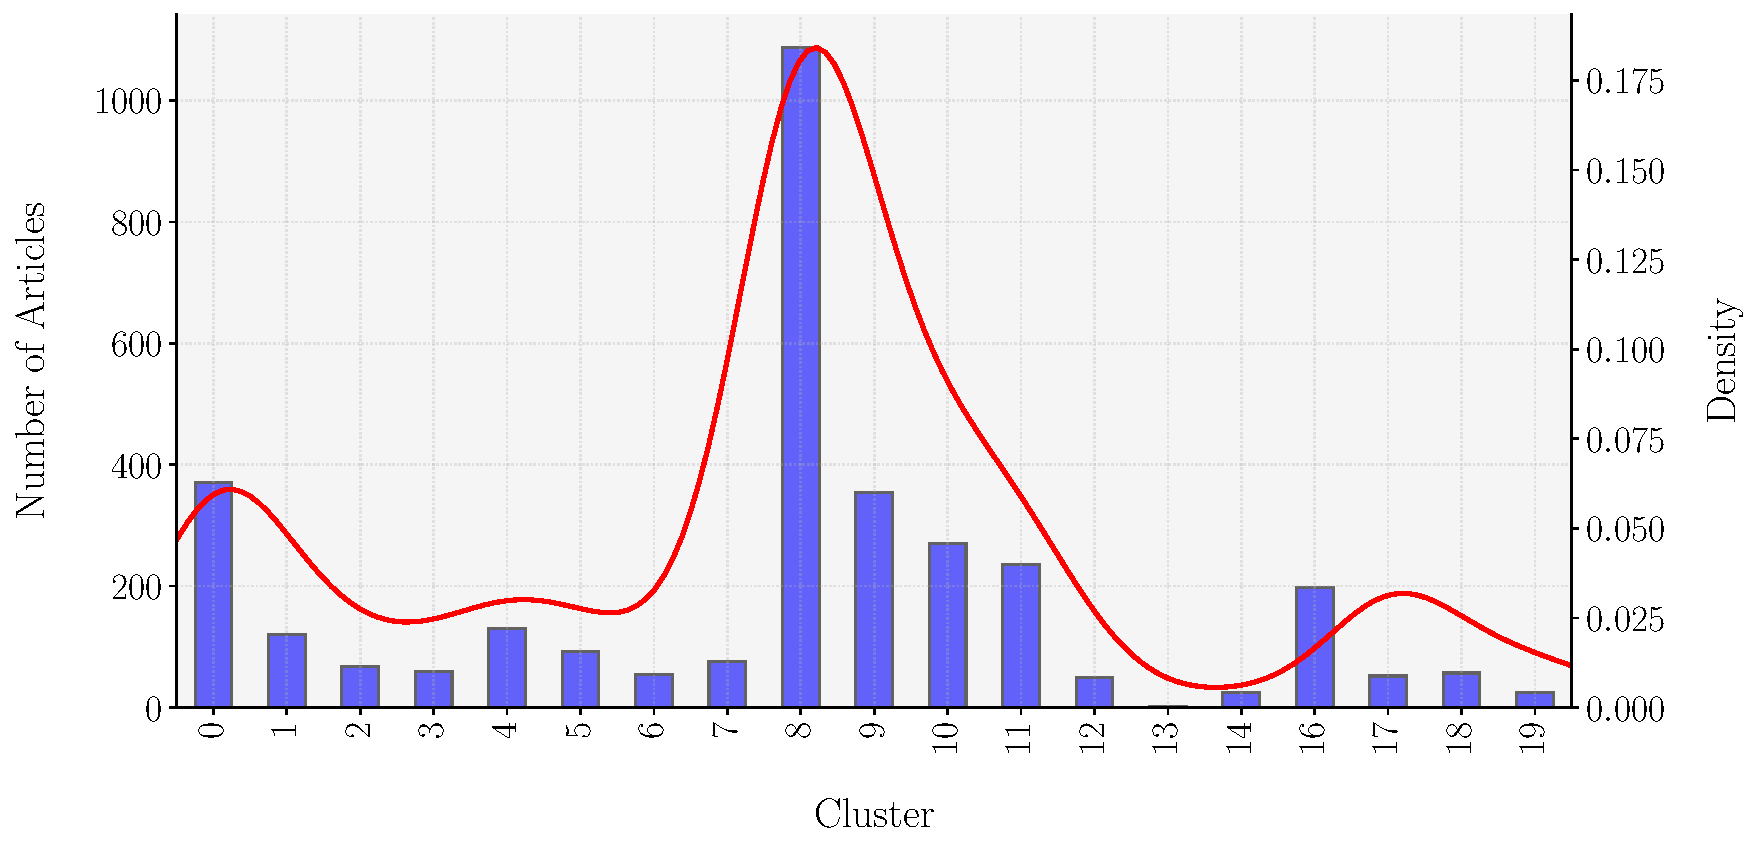
\includegraphics[scale=0.48]{fig_6a_LLAMA_Cluster_Distribution.pdf}
        \label{fig:all_data}
    \end{subfigure}

    % Lower plots
    \begin{subfigure}[b]{0.32\textwidth}
        \caption{Training data ($\D^{tr}$)}
        \centering
        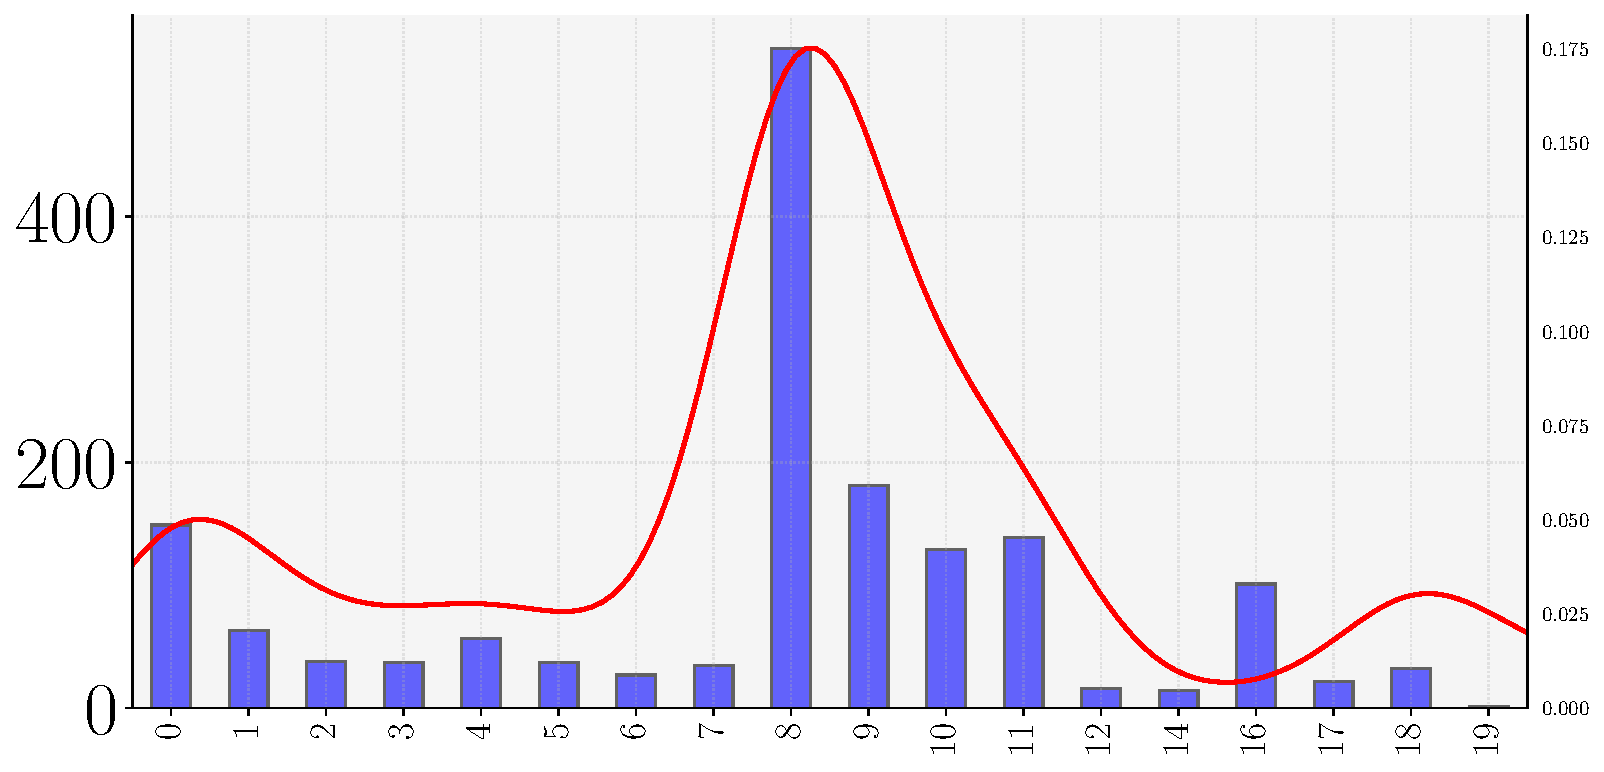
\includegraphics[width=\textwidth]{fig_6b_LLAMA_Cluster_Distribution_Train.pdf}
        \label{fig:train_data}
    \end{subfigure}
    \begin{subfigure}[b]{0.32\textwidth}
        \caption{Validation data ($\D^{val}$)}
        \centering
        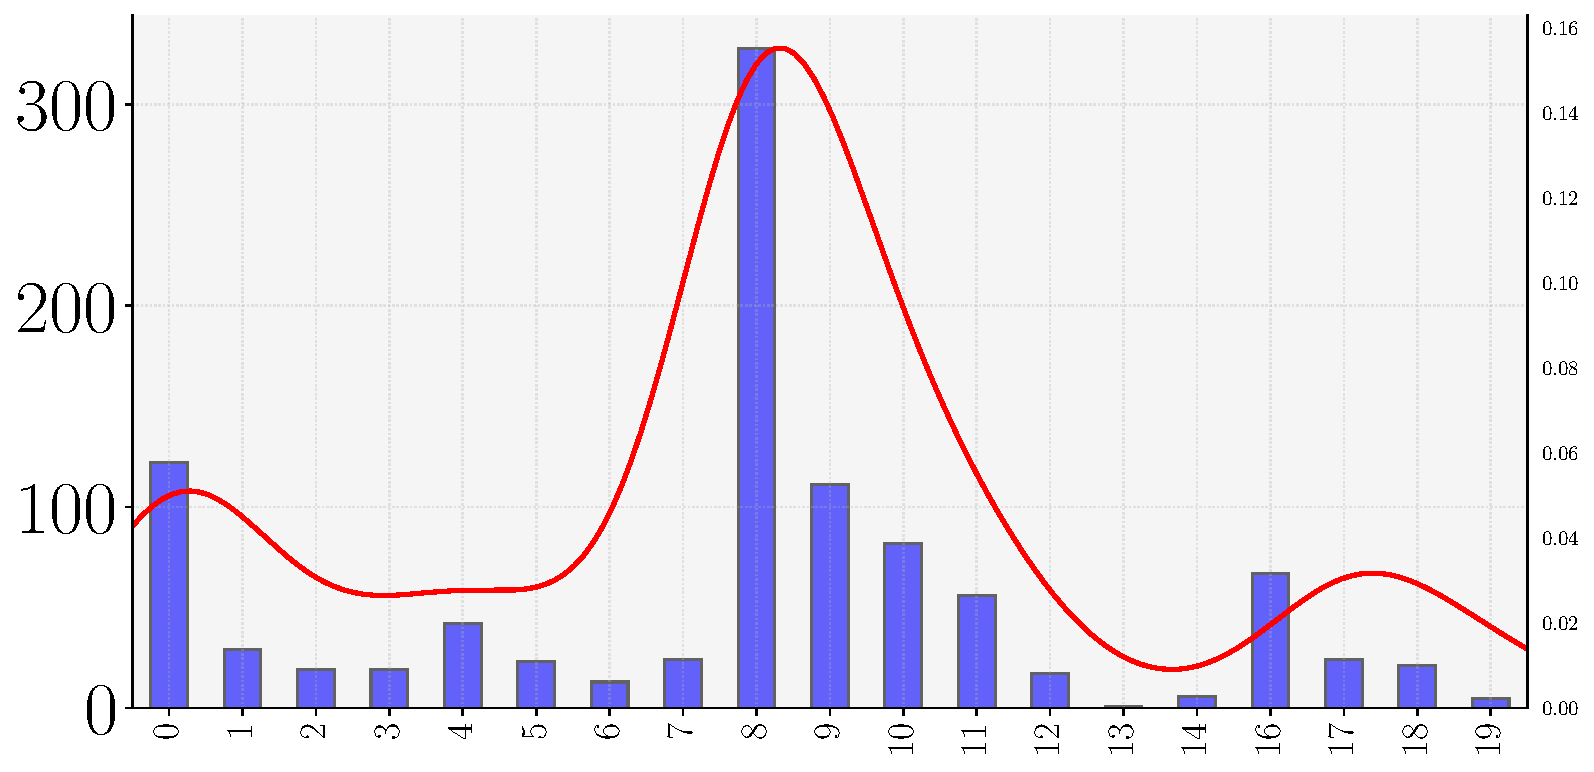
\includegraphics[width=\textwidth]{fig_6c_LLAMA_Cluster_Distribution_Validation.pdf}
        \label{fig:val_data}
    \end{subfigure}
    \begin{subfigure}[b]{0.32\textwidth}
        \caption{Test data ($\D^{test}$)}
        \centering
        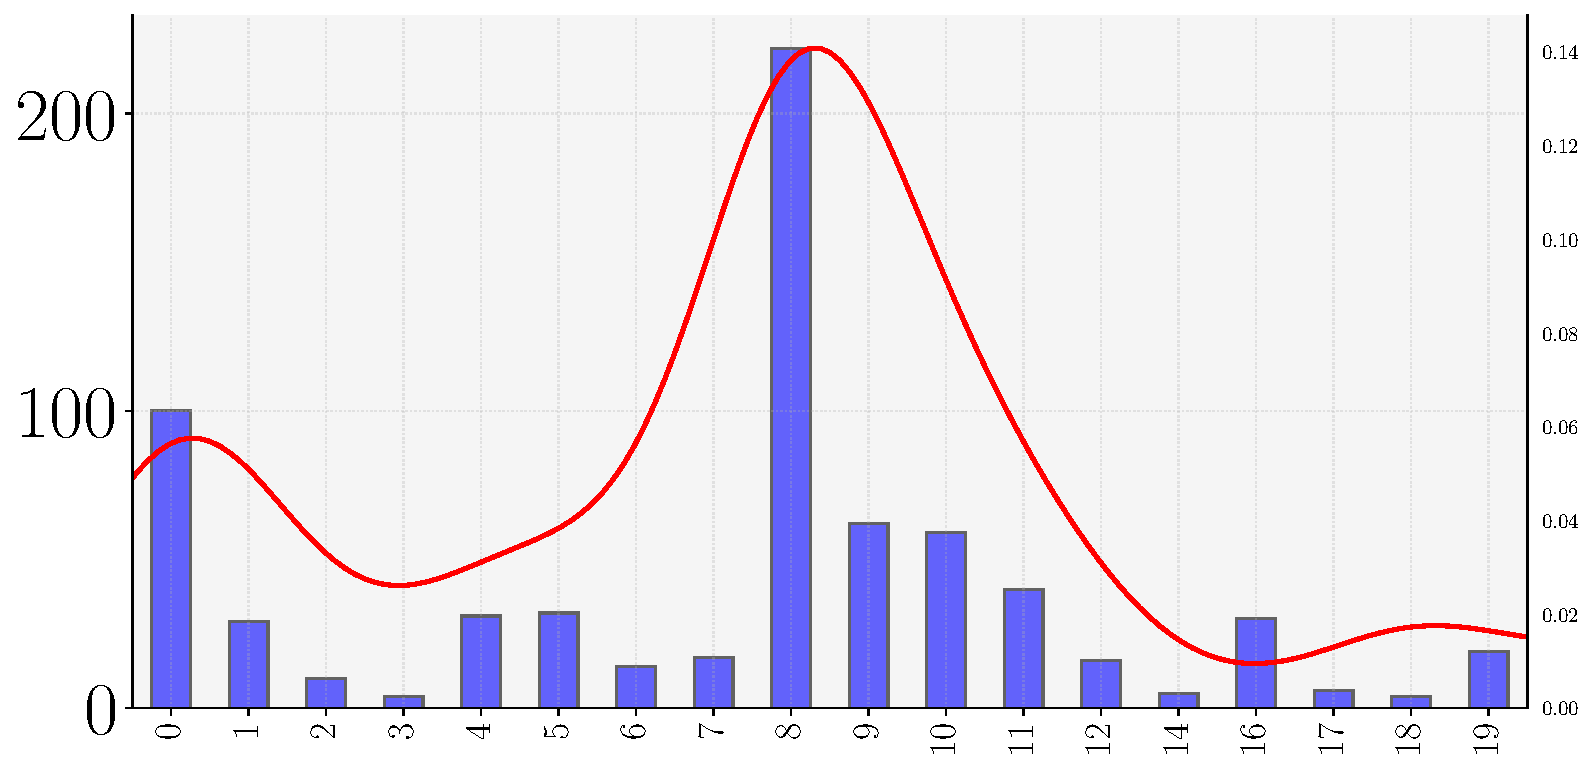
\includegraphics[width=\textwidth]{fig_6d_LLAMA_Cluster_Distribution_Test.pdf}
        \label{fig:test_data}
    \end{subfigure}
    \label{fig:LLM_cluster_distribution}
    \subcaption*{\textit{Note: This figure presents the distribution of news articles across clusters derived using an LLM-based approach. The upper plot shows the distribution for the entire dataset ($\mathcal D$), while the lower plots display the distributions for the training ($\D^{tr}$), validation ($\D^{val}$), and test ($\D^{test}$) datasets. Clusters 8, 9, 10, and 11, which capture financial events or shocks, dominate the distribution, with cluster 8 (\textit{financial, minor, positive}) representing approximately one-third of the dataset. This cluster includes articles related to financial reports with mildly positive outcomes, potentially offering insight for long trading signals. Unlike KMeans clustering with embeddings, this LLM-based clustering shows stable distributions across data splits, highlighting the robustness of this method over time. }}
\end{figure}
%----------------------------------------------------
%----------------------------------------------------


%----------------------------------------------------




\section{Trading Strategy}

%----------------------------------------------------
\subsection{Beta-neutral positions on every $(i,j)\in\mathcal B$}
Since we are interested in the individual effect of an article $i\in\D$ in each of the affected firms $j\in\F^i$, we work with the set
$
\mathcal{B}:=\3{(i,j) \mid i\in \D ~\wedge~j\in \F^i }
$, where $\abs{\mathcal{B}}=3410>\abs{\D}=2613$. 
We then fit a market model to each unique pair $(i,j)\in \mathcal{B}$
on a lookback window of 100 days with a buffer of 10 days before the effective treatment date $\tilde d_0^i$. %$\mathcal{M}^i\subset \tilde{\mathfrak{d}}$ before the effective treatment day,%
%------------------- START FOOTNOTE-------------------
%\footnote{$\mathcal M_i$ is a window of $w_m=100$ days formed with a buffer of $w_b=10$ days  before the effective treatment date $\tilde d_0^i$. Formally, it is defined as   
%$
%\mathcal{M}^i := 
%\{
%d\in \tilde{\mathfrak{d}}
%\mid 
%\mathbb{I}^{-1}_{\tilde{\mathfrak{d}}} 
%(
%\mathbb{I}_{\tilde{\mathfrak{d}}} (\tilde{d}_0^i) - {w}_b - {w}_m 
%)
%\leq d \leq 
%\mathbb{I}^{-1}_{\tilde{\mathfrak{d}}} 
%(
%\mathbb{I}_{\tilde{\mathfrak{d}}} (\tilde{d}_0^i) - {w}_b 
%)
%\}
%,
%$
%where $\mathbb{I}_{\tilde{\mathfrak d}}$ maps an element $d\in\tilde{\mathfrak d}$ to its position in $\tilde{\mathfrak d}$ and $\mathbb{I}^{-1}_{\tilde{\mathfrak d}}$ does the inverse mapping. 
%}
%%
%----------------------------------------------------
%
$$
r_{d}^{j} = \alpha^{(i,j)} + \beta^{(i,j)} r_{d}^M + \epsilon_{ d}^{(i,j)} 
%\qquad  
%\forall d \in \mathcal{M}^i
,
$$
where 
$r_{d}^{j}$ denotes the return of firm $j$ at trading day $d$ in excess of the risk-free asset, which we take to be the daily euro short-term rate (\texttt{\euro STR}),
and 
$r_{d}^M$ denotes the excess return of the market (IBEX-35).  
%----------------------------------------------------
These returns are obtained from adjusted close prices, which correct the price evolution for corporate actions such as dividends, stock splits, and new stock issuance.
%\footnote{
%The adjusted close price ensures that the returns reflect the true economic gains or losses for an investor holding the stock. 
%%
%Formally, the return of firm $j$ between two trading days $d_1, d_2\in \tilde{\mathfrak{d}}$ is computed as:
%$
%r_{d_1:d_2}^{j} = 
%(
%p_{d_2}^{j,\text{adj}} - p_{d_1}^{j,\text{adj}}
%)/(
%p_{d_1}^{j,\text{adj}}
%)
%$
%where $p_{d}^{j,\text{adj}}$ is the adjusted close price of firm $j$ at trading day $d$.
%}
%----------------------------------------------------
%
%\mx 
%----------------------------------------------------
The notation overload in the regression coefficients $(\alpha^{(i,j)},\beta^{(i,j)})$ emphasizes the fact that $\alpha$ and $\beta$ are specific to each pair $(i,j)\in\mathcal B$ since the market model is computed for each firm $j\in\F_{\t{IBEX-35}}$ on a lookback window of time 
	%$\mathcal{M}^i$, 
	which is particular to each article $i\in\D$.
%----------------------------------------------------

\mx 
The reason why we fit a market model to each $(i,j)\in\mathcal B$ is to then apply a market-neutral strategy as in 
\cite{chan2003stock} % Chan (2003)
and 
\cite{jiang2021pervasive}. % Jiang et al. (2021).
This is an investment approach designed to minimize or eliminate exposure to overall market movements, isolating the performance of a specific firm. 
% 
In particular, we employ a beta-neutral strategy by buying one unit of firm $j$'s stock and shorting $\beta^{(i,j)}$ units of the market index (i.e.: an ETF replicating the IBEX-35). 
%----------------------------------------------------
This hedged position harvests the idiosyncratic returns from the market model and it only makes sense when firm $j$'s returns are expected to outperform or underperform the market.\footnote{
For expected underperformance of firm $j$, reverse the beta-neutral positions: 
sell one unit of firm $j$ and buy $\beta^{(i,j)}$ units of the market index. However, note that this will be handled later by a Trading Rule $(TR)$.
\sx 
}
The position delivers abnormal returns $AR^{(i,j)}_{d}$ at some trading day $d\geq \tilde{d}_0^i$ given by
\begin{align*}
r_{d}^j -  \beta^{(i,j)} r_{d}^M = \alpha^{(i,j)} + \epsilon_{d}^{(i,j)} =: AR^{(i,j)}_{d}
.
\end{align*}
%----------------------------------------------------
The position is taken at the effective treatment date $\tilde d_0^i$ and is maintained over a holding window %$\mathcal H^i \subset \tilde{\mathfrak{d}}$ 
	consisting of $L\in\mathbb{N}$ trading days after $\tilde d_0^i$, where $L$ is set to 4 trading days.
%\footnote{The holding period of the position is defined as 
%$
%\mathcal H^i:=
%\{
%d \in \tilde{\mathfrak{d}}
%\mid 
%\tilde{d}_0^i
%\leq d \leq 
%\mathbb{I}^{-1}_{\tilde{\mathfrak{d}}}(\mathbb{I}_{\tilde{\mathfrak{d}}}(\tilde d_0^i)+L)
%\}
%$}
%----------------------------------------------------
The justification for this choice of $L$ results from the maximization of the Sharpe Ratio of the portfolio in the train and validation samples for both KMeans and LLM-based clustering.\footnote{ 
The choice of $L$ is justified in detail in \ref{sec:A2}, and the sensitivity of the trading strategy's out-of-sample performance to different values of $L$ is examined in Section \ref{sec:6} (\qquote{Robustness Checks}).
}
%----------------------------------------------------
Finally, we compute the Sharpe Ratio of each position $SR^{(i,j)}$, which we will subsequently employ to optimize cluster selection.
%----------------------------------------------------
%After having held the beta-neutral position over the holding period $\mathcal H^i$, we obtain a time series of abnormal returns $\{AR_{d}^{(i,j)}\}_{d\in\mathcal H^i}$ from where we can obtain the usual performance metrics. First, the average daily log returns are obtained as
%$$
%\mu^{(i,j)} = \frac{1}{{{L}}+1} 
%\sum_{d\in \mathcal H^i}
%\ln\4{1+AR_d^{(i,j)}}
%~,
%$$
%Then, the standard deviation is given by
%$$
%\sigma^{(i,j)}
%=
%\sqrt{
%\frac{1}{{{L}}}
%\sum_{d\in \mathcal H^i}
%[
%\ln(1+AR_d^{(i,j)}) - \mu^{(i,j)}
%]
%^2}
%~.
%$$
%
%\mx 
%And finally, the annualized Sharpe Ratio can be obtained by scaling the daily Sharpe Ratio by the square root of ${252}$, which are the typical number of trading days in a year according to the Spanish calendar. 
%$$
%SR^{(i,j)} =
%\sqrt{252}~
%\frac{
%\mu^{(i,j)}
%}{
%\sigma^{(i,j)}
%}
%~.
%$$
%----------------------------------------------------

%%%%%%%%%%%%%%%%%%%%%%%%%%%%%%%%%%%%%%%%%%%%%%%%%%%%%
\subsection{Optimal Cluster Selection}
%%%%%%%%%%%%%%%%%%%%%%%%%%%%%%%%%%%%%%%%%%%%%%%%%%%%%

After taking beta-neutral positions on each pair $(i,j)\in\mathcal B$ and holding them over $L$ days, 
%some window $\mathcal H^i$, 
we can obtain a measure of how profitable the positions are on average for articles that belong to the same cluster.
% $g\in\mathcal G$. 
For this purpose, let $\mathcal{B}_g$ denote the set of all article-firm pairs such that the article belongs to some cluster $g\in\mathcal G$. 
$$
\mathcal{B}_g:= \{(i,j) \mid (i,j)\in\mathcal{B} ~\wedge~ i \in \D_g \}
.
$$
The average Sharpe Ratio associated to each cluster is
$$
\overline{S R}_g=\frac{1}{\left|\mathcal{B}_g\right|} \sum_{(i,j) \in \mathcal{B}_g} S R^{(i,j)}
,
$$
and it provides a measure of the performance of the beta-neutral positions in each cluster. 
%
%
The distribution of cluster-average Sharpe Ratios across the different clusters is shown in Appendix \cref{fig:cluster-average-SR-by-split}. 


%%%%%%%%%%%%%%%%%%%%%%%%%%%%%%%%%%%%%%%%%%%%%%%%%%%%%
%%%%%%%%%%%%%%%%%   ALGORITHMS   %%%%%%%%%%%%%%%%%%%%
%%%%%%%%%%%%%%%%%%%%%%%%%%%%%%%%%%%%%%%%%%%%%%%%%%%%%
\mx
We then focus on developing two algorithms that optimally leverage the cluster information for our trading strategy. Our approach draws parallels with traditional portfolio sorting methods, where assets are typically arranged into deciles based on specific characteristics, and trading positions are established by going long on top deciles and short on bottom ones. Similarly, our strategy will construct self-financing portfolios based on clusters rather than individual assets: taking long positions in clusters expected to outperform and short positions in those expected to underperform.
%
To identify the optimal clusters for trading, we propose two distinct algorithmic approaches. The first approach, which we term \qquote{greedy}, selects clusters by maximizing the Sharpe Ratio within the validation dataset. The second approach, termed \qquote{stable}, utilizes a broader information set by incorporating both training and validation data, aiming to identify clusters that maintain consistent performance across both splits. In both algorithms, we impose sign restrictions to ensure that our trading positions align with the expected direction of returns.

\subsubsection{Greedy Algorithm}

The greedy selection of clusters is done in the validation sample 
$
\mathcal{B}^{val}:= \{
(i,j)\in\mathcal{B} 
 \mid 
  i \in \D^{val} \}
~,
$
from where we compute the cluster-average $\overline{S R}_g^{val}$ for each $g\in\G$.
%
%----------------------------------------------------
Define $\mathcal G_{SR^+}^{val}:=\{ g\in \mathcal G \mid \overline{SR}_g^{val} >0\}$ and $\mathcal G_{SR^-}^{val}:=\{ g\in \mathcal G \mid \overline{SR}_g^{val} <0\}$ as the sets of clusters with positive and negative Sharpe Ratios in the validation sample. Obviously, we will be interested in taking long positions when reading an article that is clustered in some $g\in \mathcal G_{SR^+}^{val}$, and short positions in clusters $g\in \mathcal G_{SR^+}^{val}$. 
%
%\mx 
%----------------------------------------------------
However, our trading strategy will not trade every cluster $g\in\G$. Instead, it will select the clusters from $\mathcal G_{SR^+}$ and $\mathcal G_{SR^-}$ that lead the to most profitable trades. 
To identify such clusters, we rank them by their average Sharpe Ratio. Define the ranking function $\mathfrak{R}: \mathcal{G} \to \3{1, \ldots, k^*}$ such that
$$
\mathfrak{R}_g^{val}
=
\sum_{h \in \mathcal{G}} 
\mathbf{1}\1{
\overline{S R}_h^{val} \geq \overline{S R}_g^{val} 
}
~,
$$
where $\mathbf{1}(\cdot)$ is the indicator function which equals 1 if the condition inside is true and 0 otherwise.

\mx
%----------------------------------------------------
The number of traded clusters on either side (long and short) will be upper-bounded by some hyperparameter of our choice $\theta \in \mathbb{N}$
%$\theta \in \{2 m \mid m \in \mathbb{N}\}$ 
which we set proportional to the number of clusters. Namely, $\theta =\integer{\rho k}$ for some $\rho\in(0,1)$, which has been set to $\rho=0.5$ to maximize the Sharpe Ratio of the trading strategy in the training and validation samples
\footnote{ The choice of $\theta$ is justified in detail in \ref{sec:A2}. The sensitivity of the trading strategy's out-of-sample performance to different values of $\theta$ is examined in Section \ref{sec:6} (\qquote{Robustness Checks}).}.
%
The actual number of traded clusters will not be exactly $\theta$ as there is a natural bound coming from the cardinalities of $\mathcal G_{SR^+}$ and $\mathcal G_{SR^-}$. Hence, the actual number of long and short-traded clusters will be
$
\theta^+ := \min(\theta, ~|\mathcal G_{SR^+}|)
~\t{and}~
\theta^- := \min(\theta, ~|\mathcal G_{SR^-}|)
.
$
%----------------------------------------------------
The set of traded clusters $\mathcal G_{\theta}$ is defined as
$$
\G_\theta := 
\3{
g \in \mathcal G 
\mid 
1\leq \mathfrak{R}_g^{val} \leq \theta^+
~\vee~ 
k^* -\theta^- < \mathfrak{R}_g^{val} \leq k^*
} 
= 
\G_{\theta}^+ \cup \G_{\theta}^-
~,
$$
where
$
\G_{\theta}^+ := 
\{ g \in\G \mid 
1\leq \mathfrak{R}_g^{val} \leq \theta^+
\}
$
is the set of long-traded clusters,
$
\G_{\theta}^- := 
\{ g \in\G \mid 
k^*-\theta^-
< \mathfrak{R}_g^{val} \leq 
k^*
\}
$
is the set of short-traded clusters 
and, clearly, $\abs{\G_{\theta}}=\theta^+ + \theta^- $.\footnote{
Alternatively, we could trade the same number of clusters in the long and short side by defining a unique 
$
\theta^* := \min\1{\theta, |\mathcal G_{SR^+}|, |\mathcal G_{SR^-}| }
%,
$
such that
$
\G_\theta := 
\3{
g \in \mathcal G 
\mid 
1\leq \mathfrak{R}_g^{val} \leq \theta^*
~\vee~ 
k^*-\theta^* < \mathfrak{R}_g^{val} \leq k^*
} 
$
and 
$\abs{\G_\theta}=2\theta^*$.
}
In Appendix \cref{alg:greedy_selection}, we can find the formal design of this algorithm.

%%%%%%%%%%%%%%%%%%%%%%%%%%%%%%%%%%%%%%%%%%%%%%%%%%%%%
\subsubsection{Stable Algorithm}
%%%%%%%%%%%%%%%%%%%%%%%%%%%%%%%%%%%%%%%%%%%%%%%%%%%%%

In this case, we prioritize the stability of the cluster rankings by ensuring that the traded clusters minimize the rank difference of the cluster-average Sharpe Ratios between the training and validation samples. 
To begin, we compute the rank of each cluster based on the average Sharpe Ratios in both the training and validation samples. This delivers $\{\mathfrak{R}_g^{tr}\}_{g\in\G}$ and $\{\mathfrak{R}_g^{val}\}_{g\in\G}$, which provides a measure of the relative performance of the clusters within each sample.

\mx 
Next, we calculate the absolute difference in ranks between the training and validation samples for each cluster, which allows us to measure the stability of each cluster's performance between the two samples
%
$$
\delta_{g} := | \mathfrak{R}_{g}^{tr} - \mathfrak{R}_{g}^{val} |
~.
$$

Clusters are then sorted based on their rank differences $\delta_{g}$ in descending order. To do this, we can simply compute the ranking of the ranking differences as
$$
\mathfrak{R}(\delta_g) := \sum_{h\in\G} \mbf{1}\1{\delta_g \geq  \delta_h }
.
$$
Next, we select the top $2\theta\in\mathbb{N}$ clusters with the smallest rank differences, indicating the most stable clusters across the training and validation samples. The selected clusters now are
%denoted as $\mathcal{G}_{\theta}$
$$
\mathcal{G}_{\theta} = 
\3{
g\in\G \c 1 \leq \mathfrak{R}(\delta_g) \leq 2\theta 
}
.
$$

Finally, we determine the sets of long and short-traded clusters based on the average Sharpe Ratios in both the training and validation samples. In particular, the set of long-traded clusters ($\mathcal{G}_{\theta}^{+}$) are the ones that have positive average Sharpe Ratios in both, training and validation samples
$$
\mathcal{G}_{\theta}^{+} = \{g \in \mathcal{G}_{\theta} \mid \overline{SR}_{g}^{tr} > 0 ~\wedge~ \overline{SR}_{g}^{val} > 0\}
,
$$
and by symmetry, short-traded clusters ($\mathcal{G}_{\theta}^{-}$) are the ones that have negative average Sharpe Ratios in both, training and validation samples
$$
\mathcal{G}_{\theta}^{-} = \{g \in \mathcal{G}_{\theta} \mid \overline{SR}_{g}^{tr} < 0 ~\wedge~ \overline{SR}_{g}^{val} < 0\}
~.
$$


This approach ensures that we select the most stable clusters for trading, reducing the risk associated with rank variability between the training and validation samples, and ensuring that the direction of the signal is consistent across the two splits. The final output consists of the sets of long-traded and short-traded clusters, which are then used to implement the trading strategy.
%
%
The implementation of the algorithm is methodically presented in Appendix \cref{alg:rank_stability}


%%%%%%%%%%%%%%%%%%%%%%%%%%%%%%%%%%%%%%%%%%%%%%%%%%%%%
%%%%%%%%%%%%%%%%%%   KMEANS   %%%%%%%%%%%%%%%%%%%%%%%
%%%%%%%%%%%%%%%%%%%%%%%%%%%%%%%%%%%%%%%%%%%%%%%%%%%%%
%----------------------------------------------------
\inserthere{tab:KMeans_Clusters_Signal}

\begin{table}[H]
\centering
{\fontsize{11}{12.5}\selectfont
\caption{Mapping of embeddings-based KMeans clusters to Trading Signals}
%\begin{tabular}{|c|L{13cm}|c|c|} 
\begin{tabular}{cL{13cm}cc} 
\hline \Xhline{2\arrayrulewidth}
%\rowcolor{gray!10}
\multicolumn{2}{c}{\textbf{Cluster}} & \textbf{Greedy} & \textbf{Stable} \\ \hline \Xhline{2\arrayrulewidth}
0 & Miscellaneous (Colonial, Acciona, Amadeus, Grifols, Endesa, IAG, Bankinter...) &  \textcolor{darkred}{\textsc{short}} &  \\ \hline
1 & Quarterly \& Semi-Annual Earnings Reports &  \textcolor{darkred}{\textsc{short}} &  \\ \hline
2 & BBVA \& Sabadell: Financial Performance \& Strategic Movements &  \textcolor{darkred}{\textsc{short}} &  \\ \hline
3 & Telef�nica \& Cellnex: Telecommunications Tower Sales \& Market Dynamics &  \textcolor{darkgreen}{\textsc{long}} & \textcolor{darkgreen}{\textsc{long}} \\ \hline
4 & CaixaBank: Mergers and Strategic Moves in the Banking Sector &   &  \\ \hline
5 & Telef�nica, Indra, \& M�sM�vil: Regulatory and Strategic Moves in Telecom &  \textcolor{darkgreen}{\textsc{long}} &  \\ \hline
6 & Siemens Gamesa: Supply Agreements, Profitability Targets in Renewable Energy &  \textcolor{darkred}{\textsc{short}} &  \\ \hline
7 & Cellnex: Strategic Acquisitions and Financial Moves in Telecom Infrastructure &  \textcolor{darkgreen}{\textsc{long}} &  \\ \hline
8 & Acciona, Endesa, Enag�s \& Naturgy: Strategic Moves \& Regulatory Developments in the Energy Sector &  \textcolor{darkgreen}{\textsc{long}} &  \\ \hline
9 & Repsol: Strategic Moves and Challenges in the Energy Sector &  \textcolor{darkgreen}{\textsc{long}} &  \\ \hline
10 & Ferrovial, Acciona: Strategic Expansions and Financial Maneuvers in Infrastructure &  \textcolor{darkred}{\textsc{short}} & \textcolor{darkred}{\textsc{short}} \\ \hline
11 & Solaria: Strategic Moves and Market Challenges in Renewable Energy &  \textcolor{darkgreen}{\textsc{long}} & \textcolor{darkgreen}{\textsc{long}} \\ \hline
12 & Iberdrola: Strategic Collaborations and Renewable Energy Developments &  \textcolor{darkred}{\textsc{short}} &  \\ \hline
13 & IAG: Financial Performance &  \textcolor{darkgreen}{\textsc{long}} &  \\ \hline
14 & Santander \& CaixaBank: Financial Moves and Sustainability Initiatives &  \textcolor{darkred}{\textsc{short}} &  \\ \hline
15 & ACS \& Acciona: Strategic Movements and Infrastructure Projects &  \textcolor{darkred}{\textsc{short}} & \textcolor{darkred}{\textsc{short}} \\ \hline
16 & Telef�nica: Financial Performance and Strategic Moves &  \textcolor{darkgreen}{\textsc{long}} &  \\ \hline
17 & Meli� and Spanish Tourism Sector: Challenges Amidst the Pandemic &  \textcolor{darkred}{\textsc{short}} &  \\ \hline
18 & Takeover Bids for Naturgy and M�sM�vil &  \textcolor{darkred}{\textsc{short}} &  \\ \hline
19 & Naturgy: Financial Performance &  \textcolor{darkred}{\textsc{short}} & \textcolor{darkred}{\textsc{short}} \\ \hline
20 & PharmaMar, Grifols: Regulatory Approvals and Market Moves in the Pharmaceutical Sector &  \textcolor{darkgreen}{\textsc{long}} & \textcolor{darkgreen}{\textsc{long}} \\ \hline
21 & Repsol: Financial Performance &  \textcolor{darkgreen}{\textsc{long}} & \textcolor{darkgreen}{\textsc{long}} \\ \hline
22 & Aena: Financial Performance &  \textcolor{darkgreen}{\textsc{long}} & \textcolor{darkgreen}{\textsc{long}} \\ \hline
23 & Enag�s, Endesa, Iberdrola, Red El�ctrica: Regulatory and Market Challenges in the Energy Sector &  \textcolor{darkred}{\textsc{short}} &  \\ \hline
24 & BBVA, CaixaBank, Banco Sabadell: Layoffs and Restructuring &  \textcolor{darkgreen}{\textsc{long}} & \textcolor{darkgreen}{\textsc{long}} \\ \hline
25 & Inditex, Acerinox: Market Performance and Strategic Developments in the Post-Covid Context &  \textcolor{darkred}{\textsc{short}} & \textcolor{darkred}{\textsc{short}} \\ \hline \Xhline{2\arrayrulewidth}
\end{tabular}
\label{tab:KMeans_Clusters_Signal}
}
\subcaption*{\textit{
{ Note: Mapping of embeddings-based KMeans clusters to their Trading Signal \textsc{(long/short)} for the two proposed cluster-selection algorithms (Greedy and Stable). The Greedy algorithm longs (shorts) clusters that maximize (minimize) the cluster-average-$SR$ in the validation sample subject to a positivity (negativity) constraint, while the Stable algorithm longs (shorts) clusters that minimize the rank difference between the training and validation rankings of the cluster-average-$SR$'s subject to a positivity (negativity) constraint, which is now imposed on both sample splits. In both algorithms, the cardinality of each leg is upper-bounded by a hyperparameter $\theta$. Cluster labels are proposed based on the articles they pool. 
}
}}
\end{table}
%----------------------------------------------------
In Table \ref{tab:KMeans_Clusters_Signal} we show the 26 clusters with their proposed names (based on the articles they pool together as shown in Appendix \cref{tab:KMeans_Articles_3_English}) and the selection of long and short-traded clusters according to each algorithm: \qquote{greedy} and \qquote{stable}. We write ``\textsc{long}'' for those clusters $g\in\G_\theta^+$ and ``\textsc{short}'' for $g\in\G_\theta^-$. 
%
%\mx 
As we can see, trading clusters of news articles based on this procedure is quite risky, as there is a high reliance of the signal on the past performance of a cluster. For example, clusters 21 and 22 are linked to the financial performance of Repsol and Aena, respectively, during the training and validation samples. Evidently, the future performance of these firms can change, but the signal provided by the algorithm will still indicate ``\textsc{long}''. 
%
%\bx 
Additionally, some clusters are heavily built on specific events of the period of time they were constructed upon. For example, cluster 17 pools articles related to the challenges of the tourism industry in Spain in Covid times, and cluster 25 is related to the post-covid developments of Inditex and Acerinox. Thus, a clustering approach based on embeddings is not generalizable over time. As the world evolves, clusters become outdated and require constant recalibration to maintain their relevance and predictive power. Hence, any trading strategy based solely on historical cluster performance is likely to produce misguided trading signals over time 

%%%%%%%%%%%%%%%%%%%%%%%%%%%%%%%%%%%%%%%%%%%%%%%%%%%%%
%%%%%%%%%%%%%%%%%%%%%%%%%%%%%%%%%%%%%%%%%%%%%%%%%%%%%
%%%%%%%%%%%%%%%%%%%%   LLM   %%%%%%%%%%%%%%%%%%%%%%%%
%%%%%%%%%%%%%%%%%%%%%%%%%%%%%%%%%%%%%%%%%%%%%%%%%%%%%
%%%%%%%%%%%%%%%%%%%%%%%%%%%%%%%%%%%%%%%%%%%%%%%%%%%%%
%----------------------------------------------------
\inserthere{tab:LLM_cluster_mapping_extended}

\begin{table}[H]
\caption{Mapping of LLM-based clusters to Trading Signals}
\centering
%{\footnotesize
\begin{tabular}{C{1cm}lcc}
\hline \Xhline{2\arrayrulewidth}
%\rowcolor{gray!10}
 \multicolumn{2}{c}{\textbf{Cluster}} & \textbf{Greedy} & \textbf{Stable} \\ \hline \Xhline{2\arrayrulewidth} 
0 & {(demand, minor, positive)} &  &  \\ \hline
1 & {(demand, minor, negative)} &  & \textcolor{darkred}{\textsc{short}} \\ \hline
2 & {(demand, major, positive)} & \textcolor{darkred}{\textsc{short}} & \textcolor{darkred}{\textsc{short}} \\ \hline
3 & {(demand, major, negative)} & \textcolor{darkgreen}{\textsc{long}} & \textcolor{darkgreen}{\textsc{long}} \\ \hline
\Xhline{2\arrayrulewidth}
4 & {(supply, minor, positive)} & \textcolor{darkgreen}{\textsc{long}} &  \\ \hline
5 & {(supply, minor, negative)} & \textcolor{darkred}{\textsc{short}} &  \\ \hline
6 & {(supply, major, positive)} & \textcolor{darkgreen}{\textsc{long}} &  \\ \hline
7 & {(supply, major, negative)} & \textcolor{darkred}{\textsc{short}} &  \\ \hline
\Xhline{2\arrayrulewidth}
8 & {(financial, minor, positive)} & \textcolor{darkgreen}{\textsc{long}} & \textcolor{darkgreen}{\textsc{long}} \\ \hline
9 & {(financial, minor, negative)} &  & \textcolor{darkred}{\textsc{short}} \\ \hline
10 & {(financial, major, positive)} & \textcolor{darkgreen}{\textsc{long}} &  \\ \hline
11 & {(financial, major, negative)} & \textcolor{darkred}{\textsc{short}} &  \\ \hline
\Xhline{2\arrayrulewidth}
12 & {(technology, minor, positive)} & \textcolor{darkgreen}{\textsc{long}} &  \\ \hline
13 & {(technology, minor, negative)} &  &  \\ \hline
14 & {(technology, major, positive)} & \textcolor{darkred}{\textsc{short}} &  \\ \hline
15 & {(technology, major, negative)} &  &  \\ \hline
\Xhline{2\arrayrulewidth}
16 & {(policy, minor, positive)} & \textcolor{darkred}{\textsc{short}} & \textcolor{darkred}{\textsc{short}} \\ \hline
17 & {(policy, minor, negative)} & \textcolor{darkred}{\textsc{short}} & \textcolor{darkred}{\textsc{short}} \\ \hline
18 & {(policy, major, positive)} & \textcolor{darkred}{\textsc{short}} & \textcolor{darkred}{\textsc{short}} \\ \hline
19 & {(policy, major, negative)} & \textcolor{darkred}{\textsc{short}} & \textcolor{darkred}{\textsc{short}} \\ \hline
\Xhline{2\arrayrulewidth}
\end{tabular}
%}
\vspace{0.5cm}
\subcaption*{\textit{
Note: Mapping of LLM-based clusters to their Trading Signal \textsc{(long/short)} for the two proposed cluster-selection algorithms (Greedy and Stable). The Greedy algorithm longs (shorts) clusters that maximize (minimize) the cluster-average-$SR$ in the validation sample subject to a positivity (negativity) constraint, while the Stable algorithm longs (shorts) clusters that minimize the rank difference between the training and validation rankings of the cluster-average-$SR$'s subject to a positivity (negativity) constraint, which is now imposed on both sample splits. In both algorithms, the cardinality of each leg is upper-bounded by a hyperparameter $\theta$. Each cluster corresponds to a type of news-implied firm-specific shock identified by our LLM according to the function calling schema.
}}
\label{tab:LLM_cluster_mapping_extended}
\end{table}
%----------------------------------------------------
%\mx 
%\hspace{0.5cm}
In contrast, our LLM-based clustering methodology offers significant advantages by focusing on the fundamental nature of economic shocks rather than historical patterns. This approach provides more robust and generalizable signals that are less susceptible to temporal changes in market conditions. Moreover, unlike the black box nature of vector embeddings, our methodology offers transparency and interpretability in signal generation. This is evident in how the \textit{Greedy} algorithm's cluster selection closely aligns with the direction of economic shocks: negative shocks typically correspond to price decreases and positive shocks to increases. 

Looking at \cref{tab:LLM_cluster_mapping_extended}, we observe that both algorithms consistently short articles classified as policy shocks, regardless of direction, while going long on cluster 8, which contains approximately one-third of news articles (those categorized as undergoing financial minor and positive shocks). This consistent shorting of policy shocks likely reflects markets' general aversion to policy uncertainty, as policy changes --even positive ones-- often create implementation uncertainty and take time for market participants to fully price in. Interestingly, both algorithms also exhibit seemingly counter-intuitive behavior by going long on negative major demand shocks and short on positive major demand shocks. This pattern might suggest a ``mean reversion'' expectation in the algorithms, where major demand shocks are viewed as temporary deviations that will eventually correct: negative shocks present buying opportunities, while positive shocks signal potential overvaluation.

%%%%%%%%%%%%%%%%%%%%%%%%%%%%%%%%%%%%%%%%%%%%%%%%%%%%%
\subsection{Trading Rule \& Portfolio Construction}
%%%%%%%%%%%%%%%%%%%%%%%%%%%%%%%%%%%%%%%%%%%%%%%%%%%%%
For a given selection of clusters $\G_{\theta}^+$ and $\G_{\theta}^-$, we launch trades and hold them for $L=4$ trading days.
%$L\in\mathbb{N}$ trading days over a window $\mathcal H^i$.
%
Formally, the trading rule
% $TR_{{{L}},\theta}\angl{(i,j),d}$ 
 for a pair $(i,j)\in\mathcal{B}$ at trading day ${d}\in\tilde{\mathfrak d}$ is 
%
%----------------------------------------------------
\begin{align*}
TR_{{{L}},\theta}\angl{(i,j),{d}} := \mycases{rllllll}{
+1
&\IF 
&
[
(i,j)\in\mathcal{B}_g
~\wedge~
g \in \G_{\theta}^+
]
~\wedge~
%{d}\in \mathcal H^i
d \in (\tilde d_0^i, \tilde d_0^i + L]
\\
0
&\IF
&
[
(i,j)\in\mathcal{B}_g
~\wedge~
g \not\in \G_\theta ~
]
~\vee~
%{d} \not\in \mathcal H^i
d \not\in (\tilde d_0^i, \tilde d_0^i + L]
\\
-1
&\IF 
&
[
(i,j)\in\mathcal{B}_g
~\wedge~
g \in \G_{\theta}^-
]
~\wedge~
%{d} \in \mathcal H^i
d \in (\tilde d_0^i, \tilde d_0^i + L]
}
~.
\end{align*}
%----------------------------------------------------

In this context, a portfolio is a collection of positions taken in a firm's stocks according to $TR_{{{L}},\theta}\angl{(i,j),{d}}$. In other words, it is the set of all $\angl{(i,j),{d}}$ for which a trade is executed. 
\begin{align*}
\mathcal P:= 
\3{\angl{(i,j),{d}} 
\c 
(i,j)\in\mathcal{B} 
~\wedge~
{d}\in \tilde{\mathfrak{d}}
~\wedge~
TR_{{{L}},\theta}\angl{(i,j),{d}} \neq 0
}
.
\end{align*}
The set of open positions on a particular day ${d}\in\tilde{\mathfrak d}$ is defined as
$$
\mathcal{P}_{ d}
:=
\3{
(i, j) \in \mathcal{B} 
\c 
T R_{L, \theta}\langle(i, j), {d}\rangle \neq 0 
}
,
$$
and the portfolio is rebalanced every day, so each position $(i, j)\in \mathcal{P}_{d}$ receives a weight that is inversely proportional to the total amount of open positions in that day (i.e. $1/|\mathcal{P}_{d}|$).\footnote{
Note that the cardinality of the set of open positions at day ${d}\in\tilde{\mathfrak d}$, denoted as $|\mathcal{P}_{d}|$, can be computed as the sum of the absolute values of the trading rule over all pairs $(i,j)\in\mathcal B$
 for a given trading day $d\in\tilde{\mathfrak{d}}$.
$$
|\mathcal{P}_{ d}|=\sum_{(i,j)\in\mathcal B}
\abs{
TR_{L, \theta}\angl{(i,j),  d}
}
~.
$$
}
This produces an equally-weighted rolling-portfolio similar to 
\cite{jegadeesh1993returns} % Jegadeesh and Titman (1993)
and 
\cite{chan2003stock}. % Chan (2003)
%
The overlapping returns of the portfolio at $d\in\tilde{\mathfrak{d}}$ can be obtained as an average of the abnormal returns weighted by the trading rule, which determines the direction of each position (long or short), and scaled by the number of open positions in that day,
$$
r_{d}^{\mathcal{P}} 
:= 
\frac{1}{|\mathcal{P}_{d}|}
\sum_{(i, j), \in \mathcal{P}_{d}}
T R_{{{L}}, \theta}\angl{(i,j), {d}} 
\cdot 
AR_{{d}}^{(i,j)}
~.
$$

%%%%%%%%%%%%%%%%%%%%%%%%%%%%%%%%%%%%%%%%%%%%%%%%%%%%%
%%%%%%%%%%%%%%%%%%%%%%%%%%%%%%%%%%%%%%%%%%%%%%%%%%%%%
%%%%%%%%%%%%%%%%%%%%%%%%%%%%%%%%%%%%%%%%%%%%%%%%%%%%%
%%%%%%%%%%%%%%%%%%%%%%%%%%%%%%%%%%%%%%%%%%%%%%%%%%%%%
%Finally, defining the mean portfolio return as
%%----------------------------------------------------
%$
%\mu^{\mathcal{P}}:=
%({1}/{|\tilde{\mathfrak{d}}|})
%\sum_{\tilde{d} \in \tilde{\mathfrak{d}}} \ln (1+r_{\tilde{d}}^{\mathcal{P}})
%$
%and the associated standard deviation:
%$ 
%\sigma^{\mathcal{P}}
%:=
%\sqrt{
%({1}/{|\tilde{\mathfrak{d}}|-1})
%\sum_{\tilde{d} \in \tilde{\mathfrak{d}}}
%[\ln
%(1+r_{\tilde{d}}^{\mathcal{P}}
%)-\mu^{\mathcal{P}}]^2} 
%$
%, we can obtain the annualized Sharpe Ratio of the portfolio as
%$ SR^{\mathcal{P}} :=  \sqrt{252} ~
%{\mu^{\mathcal{P}}}/{\sigma^{\mathcal{P}}} 
%$.
%%----------------------------------------------------
%
%

%--------  Evaluating the Trading Strategy  %-----------

%
%\subsection{Evaluating the Trading Strategy}
%\hspace{0.5cm}The trading strategy is evaluated in the test sample by applying $TR\angl{(i,j),d}$ to all $(i,j)\in\mathcal{B}^{test}$. 
%This delivers the portfolio
%\begin{align*}
%\mathcal{P}^{test}=\3{\angl{(i,j),d} \c (i,j)\in \mathcal{B}^{test} ~\wedge~  TR_{L,\theta}\angl{(i,j),d} \neq 0 }
%,
%\end{align*}
%from where we can compute the portfolio returns 
%$
%r_{d}^{\mathcal{P}^{test}} = 
%({1}/{|\mathcal{P}_{d}^{test}|})
%\sum_{(i, j), \in \mathcal{P}_{d}^{test}}
%T R_{{{L}}, \theta}\angl{(i,j), {d}} 
%\cdot 
%AR_{{d}}^{(i,j)}
%,
%$
%and then obtain $\mu^{\mathcal{P}^{test}}$ and $\sigma^{\mathcal{P}^{test}}$. Finally, we evaluate the \textit{out-of-sample} performance of our trading strategy by looking at the Sharpe Ratio in the test sample
%$
%SR^{\mathcal{P}^{test}} = 
%\sqrt{252}~
%{\mu^{\mathcal{P}^{test}}}/{\sigma^{\mathcal{P}^{test}}}
%.$
%%%%%%%%%%%%%%%%%%%%%%%%%%%%%%%%%%%%%%%%%%%%%%%%%%%%%
%%%%%%%%%%%%%%%%%%%%%%%%%%%%%%%%%%%%%%%%%%%%%%%%%%%%%
%%%%%%%%%%%%%%%%%%%%%%%%%%%%%%%%%%%%%%%%%%%%%%%%%%%%%
%%%%%%%%%%%%%%%%%%%%%%%%%%%%%%%%%%%%%%%%%%%%%%%%%%%%%

In \cref{fig:portfolio_returns_comparison} we plot the cumulative gross returns of trading strategies based on KMeans clustering (Panel A) and LLM clustering (Panel B) across different data splits

%----------------------------------------------------
\inserthere{fig:portfolio_returns_comparison}
\begin{figure}[H]
\caption{Comparison of Cumulative Gross Returns across Clustering Approaches}
\label{fig:portfolio_returns_comparison}

% Panel A: KMeans
\begin{subfigure}{\textwidth}
\caption{Panel A: Cumulative Gross Returns of $\mathcal{P}_{\text{KMeans}}$}
\centering
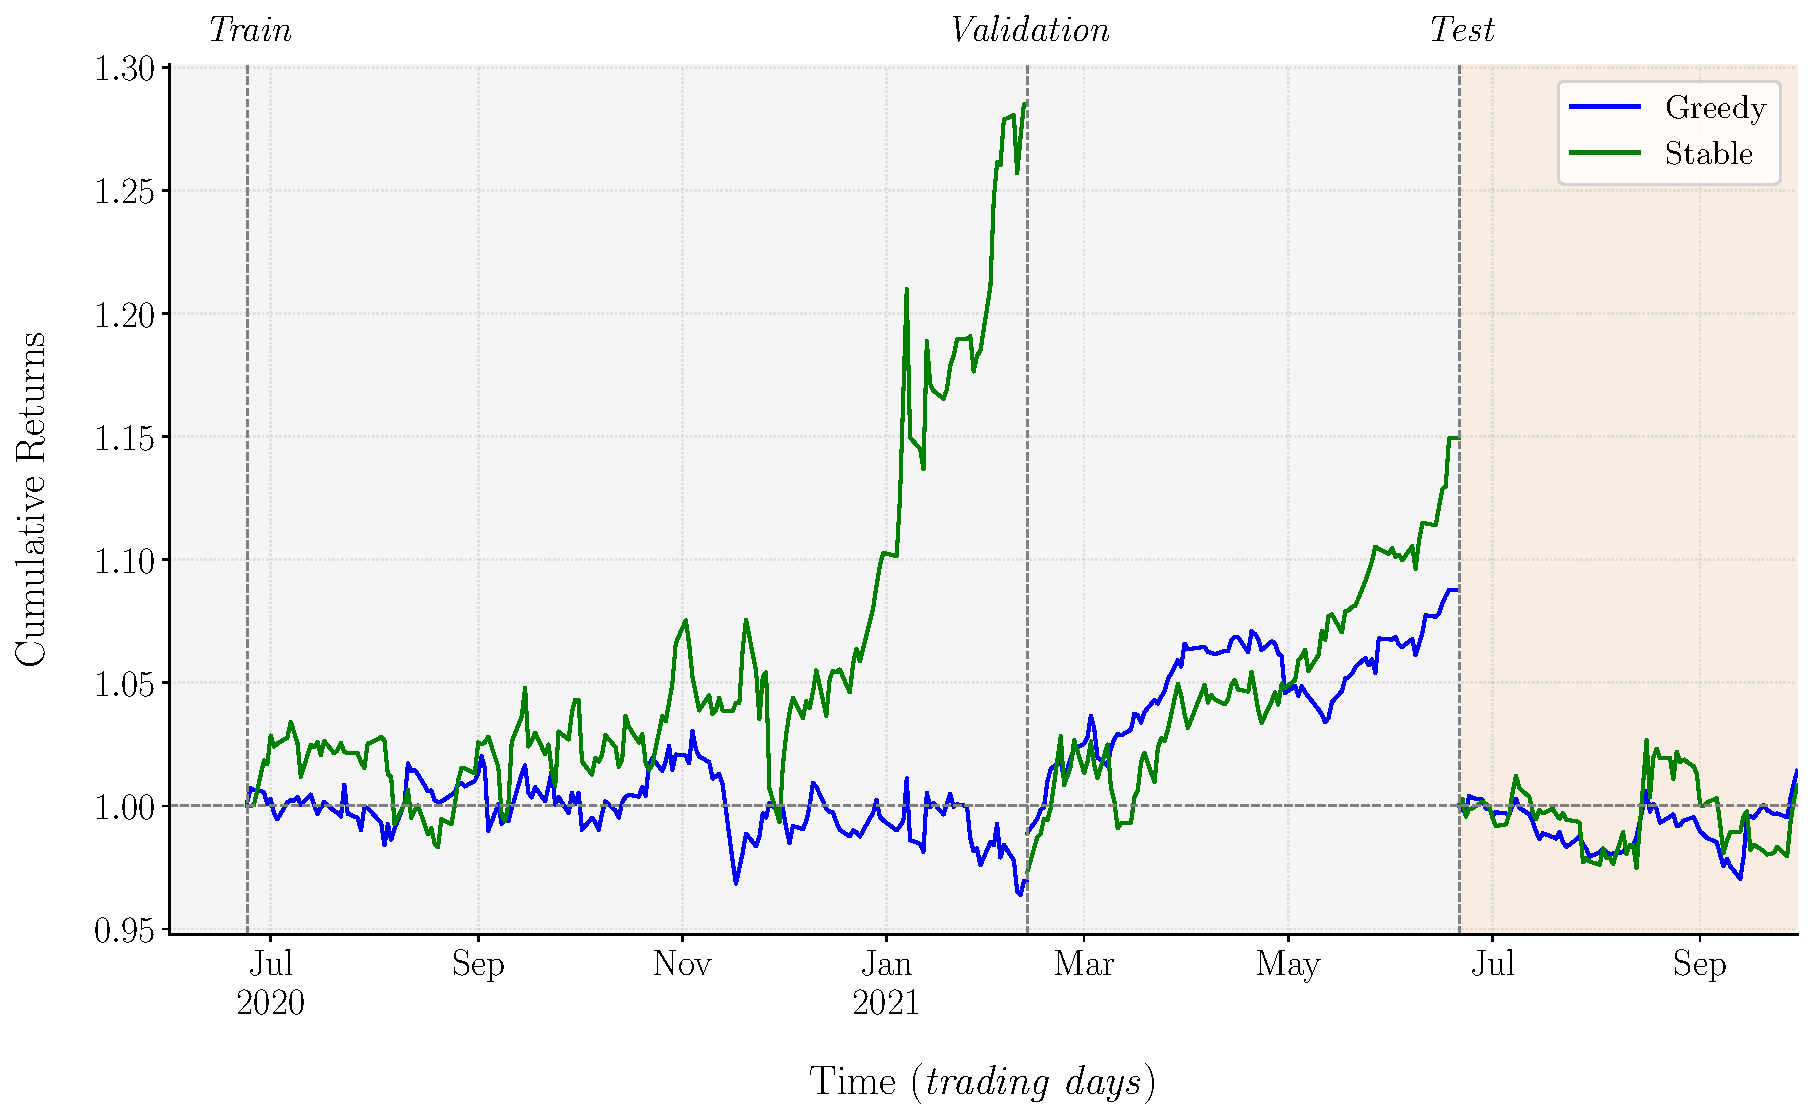
\includegraphics[scale=0.44]{fig_8a_KMeans_Portfolio.pdf}
\end{subfigure}

\vspace{0.75cm}

% Panel B: LLM
\begin{subfigure}{\textwidth}
\caption{Panel B: Cumulative Gross Returns of $\mathcal{P}_{\text{LLM}}$}
\centering
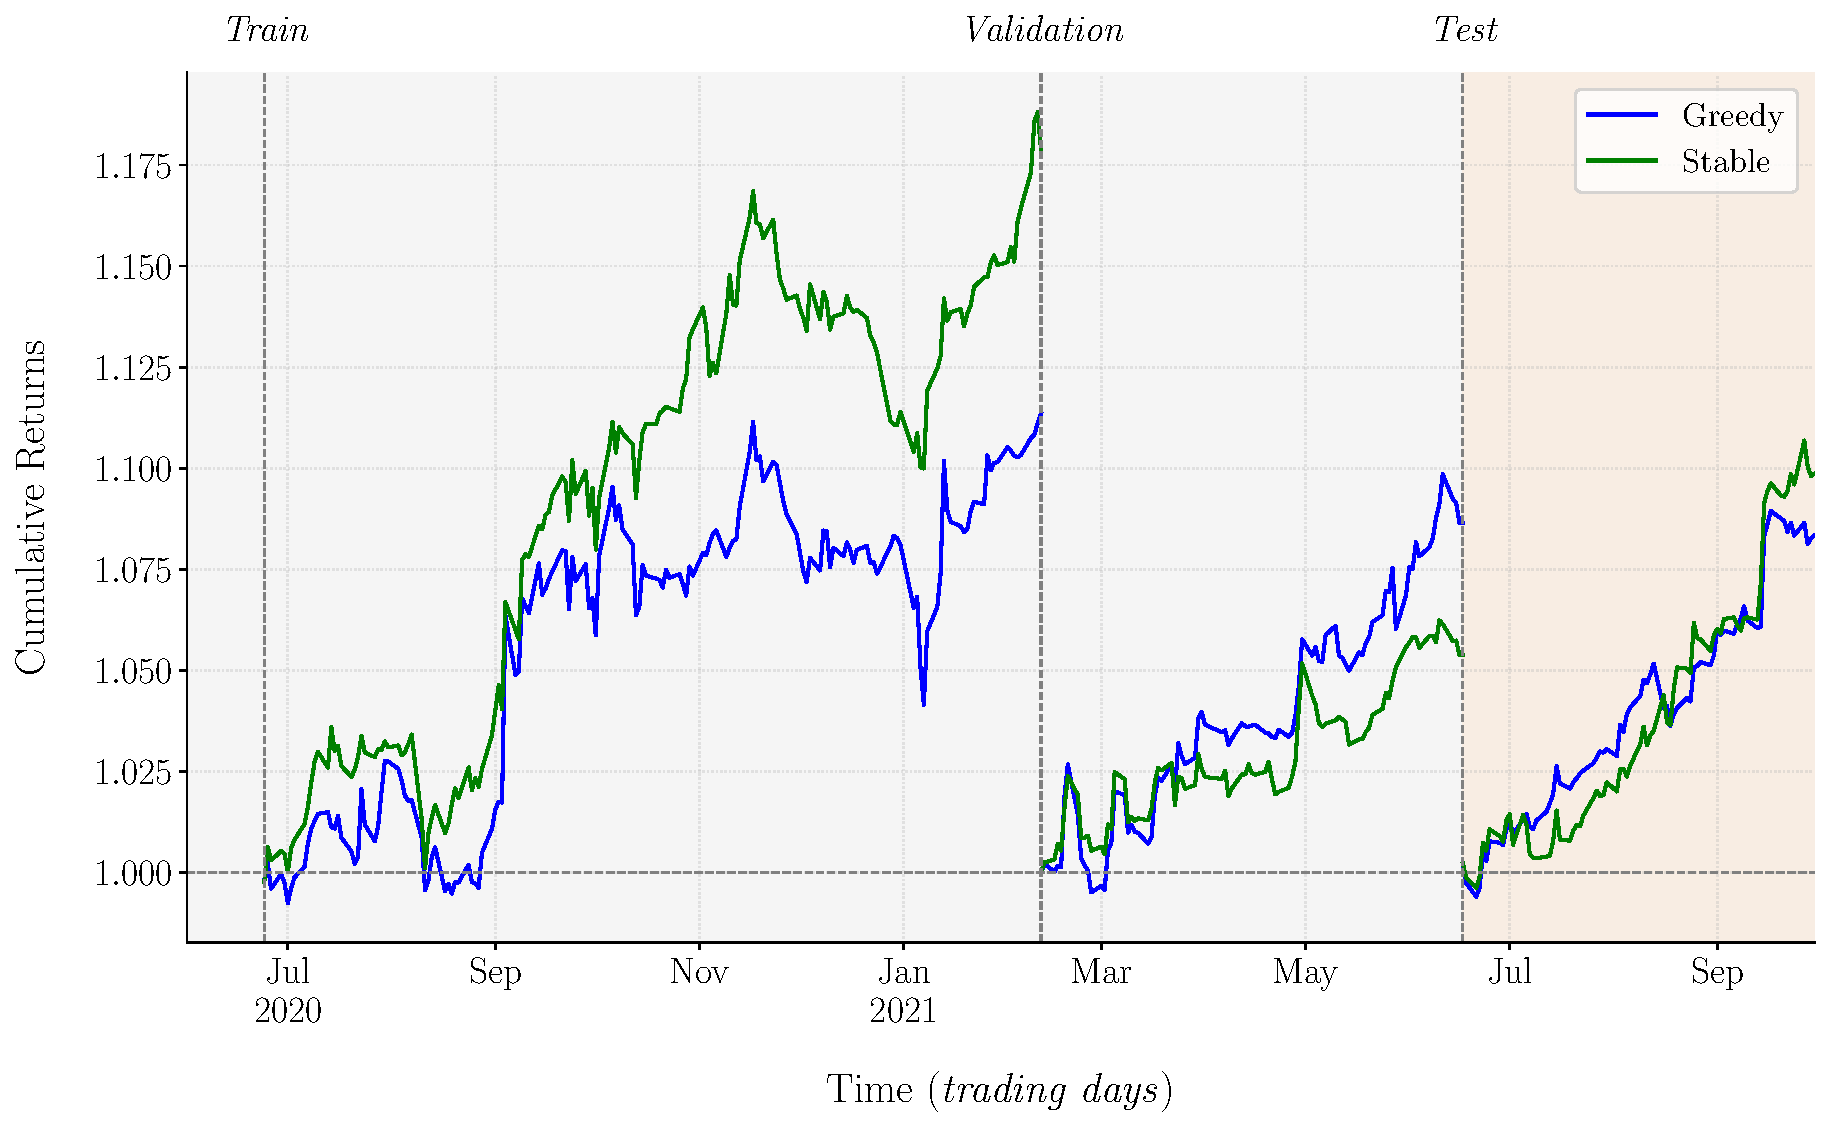
\includegraphics[scale=0.44]{fig_8b_LLAMA_Portfolio.pdf}
\end{subfigure}

\vspace{0.5cm}
\begin{minipage}{\textwidth}
\setlength{\parindent}{0pt}
{\footnotesize\textit{Note:} 
This figure presents the cumulative gross returns of trading strategies based on KMeans clustering (Panel A) and LLM clustering (Panel B) across different data splits. For both approaches, the holding period of the beta-neutral strategies is set to $L=4$ trading days. The number of traded clusters differs between approaches: $\theta=\integer{0.5k}=13$ for KMeans ($k^*=26$ clusters) and $\theta=\integer{0.5k}=10$ for LLM ($k=20$ clusters). The selection criteria for these parameters is based on maximizing the Sharpe Ratios of the train and validation samples. The Test split is higlhighted with a yellow background.
%
%The two approaches show markedly different out-of-sample performance. The embeddings-based KMeans clusters (Panel A) demonstrate poor out-of-sample performance, indicating a lack of robustness and failure to generalize effectively over time. In contrast, the LLM-based clustering approach (Panel B) exhibits strong out-of-sample performance, suggesting that the LLM-derived clusters effectively capture and predict market reactions to firm-specific economic shocks implied by news.
}
\end{minipage}
\end{figure}
%----------------------------------------------------

%%%%%%%%%%%%%%%%%%%  KMEANS %%%%%%%%%%%%%%%%%%%%%%%%%

\textbf{KMeans}. 
In panel A of \cref{tab:portfolio_statistics_gross_comparison} we show the portfolio statistics of the benchmark model.
As we can see, both algorithms work well on the data splits they were trained on: the Stable algorithm works well on both, training and validation data, while the Greedy algorithm does a good job only on validation data as expected. However, this doesn't say anything about any of these algorithms, as it is easy to make profitable trades \textit{in-sample}. 
%
The generalizability of the strategy is determined \textit{out-of-sample} in the test data. The empirical analysis reveals significant challenges in the strategy's ability to maintain consistent performance across different time periods. During the training and validation phases, the methodology shows promising results with annualized returns ranging from 26.6\% to 47.7\% and strong risk-adjusted performance metrics (Sharpe ratios between 2.0 and 3.2). However, this performance deteriorates substantially in the test period, where returns drop to modest levels (2.9\% to 4.9\% annually) with significantly lower Sharpe ratios (0.2 to 0.7), suggesting that the strategy's alpha-generating capability does not generalize well out of sample. The distributional properties of returns in the test period provide additional insights into the strategy's behavior under true out-of-sample conditions. The shift from negative to strongly positive skewness (1.85 to 2.46) coupled with high excess kurtosis (5.50 to 14.57) suggests that the strategy's return distribution has fundamentally changed, characterized by more frequent small losses offset by occasional large gains. This asymmetric return pattern, while potentially appealing from a risk preference perspective, differs markedly from the training period characteristics. The tail risk measures further illuminate the strategy's risk profile, with annualized 95\% VaR ranging from -7.8\% to -18.9\% and corresponding CVaR from -9.7\% to -26.8\% in the test period. These statistical properties, combined with the strong dependence on historical cluster-specific performance, indicate that the strategy fails to identify stable and generalizable trading signals, likely due to its reliance on firm and industry-specific clustering patterns that do not persist out of sample. As we can see in the plot, neither algorithm is able to generate a consistent profile of earnings, and the statistics confirm that profits are negligible, and would likely be eaten away by exogenous market frictions (e.g. trading costs).

%----------------------------------------------------
\inserthere{tab:portfolio_statistics_gross_comparison}

\begin{table}[H] 
\caption{Portfolio Statistics Comparison: KMeans vs LLM Clustering
% | Gross Returns
} 
\centering
\label{tab:portfolio_statistics_gross_comparison}

\renewcommand{\arraystretch}{1.1}
\newcolumntype{P}[1]{>{\centering\arraybackslash}p{#1}}

% Panel A: KMeans
\begin{subtable}{\textwidth}
\caption{Panel A: Statistics of $\mathcal{P}_{\text{KMeans}}$}
\centering
{\small
\begin{tabular}{
 P{1.28cm} P{0.9cm} P{0.9cm} P{0.9cm} P{0.9cm} P{0.9cm} P{0.9cm} 
 P{0.9cm} P{1cm} P{0.9cm} P{0.9cm} P{0.9cm} P{0.9cm}
}
\Xhline{2\arrayrulewidth}
\textbf{Split} & \textbf{Algo.} & \textbf{Cum. Ret.} & \textbf{Avg. Ret.} & \textbf{St. Dev.} & \textbf{Sharpe Ratio} & \textbf{Sortino Ratio} & \textbf{Max. DD} & \textbf{Calmar Ratio} & \textbf{Skew.} & \textbf{Exc. Kurt.} & \textbf{VaR 95\%} & \textbf{CVaR 95\%} \\
\Xhline{2\arrayrulewidth}
\multirow{2}{*}{All} & \textit{Greedy} & 1.070 & 5.3 & 9.7 & 0.5 & 0.6 & -6.9 & 0.8 & -0.45 & 4.04 & -13.7 & -22.9 \\
 & \textit{Stable} & 1.489 & 35.8 & 16.8 & 1.8 & 2.2 & -7.6 & 4.7 & 0.19 & 5.08 & -22.6 & -36.1 \\
\hline
\multirow{2}{*}{Train} & \textit{Greedy} & 0.959 & -6.2 & 11.7 & -0.5 & -0.5 & -6.9 & -0.9 & -0.52 & 2.72 & -18.3 & -28.5 \\
 & \textit{Stable} & 1.250 & 40.4 & 19.6 & 1.7 & 2.0 & -7.6 & 5.3 & -0.22 & 3.24 & -29.3 & -43.1 \\
\hline
\multirow{2}{*}{Validation} & \textit{Greedy} & 1.088 & 26.8 & 7.3 & 3.3 & 3.7 & -3.5 & 7.8 & -0.47 & 1.17 & -9.5 & -15.9 \\
 & \textit{Stable} & 1.149 & 47.6 & 13.3 & 2.9 & 3.5 & -3.6 & 13.1 & -0.19 & 1.76 & -18.3 & -28.1 \\
\hline
\multirow{2}{*}{Test} & \textit{Greedy} & 1.014 & 4.9 & 6.9 & 0.7 & 1.0 & -3.6 & 1.4 & 1.85 & 5.50 & -7.8 & -9.7 \\
 & \textit{Stable} & 1.008 & 2.9 & 14.3 & 0.2 & 0.3 & -4.6 & 0.6 & 2.46 & 14.57 & -18.9 & -26.8 \\
\Xhline{2\arrayrulewidth}
\end{tabular}
}
\end{subtable}

\vspace{0.5cm}

% Panel B: LLM
\begin{subtable}{\textwidth}
\caption{Panel B: Statistics of $\mathcal{P}_{\text{LLM}}$}
\centering
{\small
\begin{tabular}{
 P{1.28cm} P{0.9cm} P{0.9cm} P{0.9cm} P{0.9cm} P{0.9cm} P{0.9cm} 
 P{0.9cm} P{1cm} P{0.9cm} P{0.9cm} P{0.9cm} P{0.9cm}
}
\Xhline{2\arrayrulewidth}
\textbf{Split} & \textbf{Algo.} & \textbf{Cum. Ret.} & \textbf{Avg. Ret.} & \textbf{St. Dev.} & \textbf{Sharpe Ratio} & \textbf{Sortino Ratio} & \textbf{Max. DD} & \textbf{Calmar Ratio} & \textbf{Skew.} & \textbf{Exc. Kurt.} & \textbf{VaR 95\%} & \textbf{CVaR 95\%} \\
\Xhline{2\arrayrulewidth}
\multirow{2}{*}{All} & \textit{Greedy} & 1.310 & 23.1 & 9.6 & 2.2 & 2.9 & -6.3 & 3.7 & 1.47 & 9.93 & -13.6 & -18.9 \\
 & \textit{Stable} & 1.365 & 27.0 & 8.6 & 2.8 & 3.4 & -5.9 & 4.6 & 0.28 & 2.24 & -11.9 & -16.9 \\
\hline
\multirow{2}{*}{Train} & \textit{Greedy} & 1.112 & 17.6 & 11.4 & 1.4 & 1.9 & -6.3 & 2.8 & 1.65 & 9.00 & -15.7 & -21.0 \\
 & \textit{Stable} & 1.177 & 28.3 & 9.9 & 2.5 & 3.0 & -5.9 & 4.8 & 0.16 & 1.71 & -13.5 & -19.6 \\
\hline
\multirow{2}{*}{Validation} & \textit{Greedy} & 1.091 & 28.0 & 8.2 & 3.0 & 4.0 & -3.1 & 9.1 & 0.14 & 1.37 & -10.6 & -16.8 \\
 & \textit{Stable} & 1.048 & 14.2 & 7.0 & 1.9 & 2.1 & -1.9 & 7.4 & 0.25 & 1.37 & -11.1 & -14.7 \\
\hline
\multirow{2}{*}{Test} & \textit{Greedy} & 1.084 & 30.8 & 6.2 & 4.3 & 6.0 & -1.5 & 21.0 & 1.49 & 8.30 & -6.9 & -9.9 \\
 & \textit{Stable} & 1.100 & 37.2 & 7.1 & 4.4 & 7.2 & -1.1 & 34.5 & 0.84 & 1.95 & -9.5 & -11.3 \\
\Xhline{2\arrayrulewidth}
\end{tabular}
}
\end{subtable}

\vspace{0.5cm}
\begin{minipage}{\textwidth}
\setlength{\parindent}{0pt}
{\small\textit{Note:
Portfolio statistics of trading strategies based on clusters obtained from KMeans (Panel A) and LLM (Panel B) approaches.
The statistics provided include performance metrics (Cumulative Return, Average Return (\%)), risk measures (Standard Deviation (\%), Maximum Drawdown (\%), Value at Risk (\%), Conditional Value at Risk (\%)), risk-adjusted performance ratios (Sharpe Ratio, Sortino Ratio, Calmar Ratio), and return distribution characteristics (Skewness, Excess Kurtosis). These statistics are provided for both cluster-selection algorithms: Greedy and Stable.
Except for the Cumulative Return, all returns are annualized. The Sharpe Ratio is computed using the daily returns, assuming 252 trading days in a year. The Sortino Ratio is calculated using the daily downside returns. The Maximum Drawdown is the maximum loss from a peak to a trough. The Calmar Ratio is the ratio of the annualized return to the maximum drawdown. Skewness measures the asymmetry of the return distribution, while Kurtosis quantifies the tails' thickness. The Value at Risk (VaR) and Conditional Value at Risk (CVaR) are calculated at a 95\% confidence level.
The Greedy algorithm longs (shorts) clusters that maximize (minimize) the cluster-average-$SR$ in the validation sample subject to a positivity (negativity) constraint, while the Stable algorithm longs (shorts) clusters that minimize the rank difference between the training and validation rankings of the cluster-average-$SR$'s subject to a positivity (negativity) constraint, which is now imposed on both sample splits. In both algorithms, the cardinality of each leg is upper-bounded by a hyperparameter $\theta$.
The holding period of the beta-neutral positions is set to $L$ = 4 trading days for both approaches. The number of traded clusters is $\theta = 0.5k=13$ for KMeans ($k^*=26$ clusters) and $\theta = 0.5k=10$ for LLM ($k^*=20$ clusters). The selection criteria for these hyperparameters ($L,\theta$) is based on maximizing the Sharpe Ratios of the train and validation samples.
}}
\end{minipage}
\end{table}
%----------------------------------------------------


%%%%%%%%%%%%%%%%%%%%%% LLM %%%%%%%%%%%%%%%%%%%%%%%%%%%

\mx

\textbf{LLM}. 
%In panel B of \cref{tab:portfolio_statistics_gross_comparison} we show the portfolio statistics of the LLM-based strategy.
Panel B of \cref{tab:portfolio_statistics_gross_comparison} presents the performance metrics for our LLM-based approach.
As before, both algorithms perform really well on ``seen'' data. However, different from before, the \textit{Greedy} algorithm works well also on the Training Split (which it was not trained on). More importantly, both algorithms do a great job in the test data. As we can see, both are able to achieve a consistent profile of earnings through the split. 
%
The portfolio statistics 
%in Panel B of \cref{tab:portfolio_statistics_gross_comparison} 
reveal notable consistency in the strategy's performance across different time periods. During the training and validation phases, the methodology demonstrates solid performance with annualized returns ranging from 16.0\% to 28.3\% and Sharpe ratios between 1.4 and 2.9. This performance strengthens in the test period, where returns increase to 30.8\%-37.2\% annually with Sharpe ratios of 4.3-4.4, indicating that the strategy's alpha-generating capability successfully generalizes to out-of-sample conditions. The distributional properties of returns provide evidence for the strategy's robustness. 
%
The test period maintains positive skewness (0.84 to 1.49) and moderate to high excess kurtosis (1.95 to 8.30), indicating an asymmetric return pattern with more frequent small losses offset by larger gains. This return distribution is complemented by contained maximum drawdowns (1.1\% to 1.5\%) and strong Calmar ratios (21.0 to 34.5) in the test period. The tail risk measures further support the strategy's risk management properties, with annualized 95\% VaR ranging from -6.9\% to -9.5\%, and CVaR ranging from -9.9\% to -11.3\% in the test period. 
%
Taken together, the strategy's ability to sustain consistent out-of-sample performance metrics demonstrates that the LLM-based clustering approach identifies enduring trading signals that transcend specific market regimes.

%----------------------------------------------------

While our primary focus has been on developing a methodology to anticipate market reactions to news (i.e., identifying winners and losers to assess the predictive power of our LLM-based approach), we also analyze the trading intensity and implementation costs of the resulting strategies. The detailed examination in \ref{sec:A8} reveals that, 
%conservative
after accounting for transaction costs, the LLM-based approach maintains its superior performance relative to KMeans, though with attenuated profitability. Therefore, practitioners interested in the practical implementation of this strategy would benefit from optimizing the trading strategy by incorporating transaction costs into their framework.


%%, though with attenuated profitability. 
% Specifically, while KMeans strategies generate consistent losses out-of-sample (Sharpe Ratios of -0.6 and -0.5), our LLM-based approach maintains a high profitability %achieves near-neutral to slightly positive net returns 
% (Sharpe Ratios of 2.8 and 3.1) in the test period, with notably lower risk metrics. 
% %These results underscore that while our methodology successfully captures predictable market reactions to news, practitioners implementing such strategies would benefit from incorporating transaction costs into their optimization framework.


%%%%%%%%%%%%% ROBUSTNESS CHECKS %%%%%%%%%%%%%%%%%%

\section{Robustness Checks} \label{sec:6}

In our applications we have worked with a holding period of $L=4$ trading days and an upper bound on traded clusters of $\theta=\integer{0.5k}$. As shown in \ref{sec:A2}, such choices result from the maximization of the Sharpe Ratios in the train and validation samples. All that is left is to check whether our out-of-sample results are sensitive to the choice of hyperparameters ($L,\theta$). For this purpose, we evaluate the variability of the Sharpe Ratios of the test portfolio ($SR^{\mathcal P^{test}}$) to changes in $L$ and $\theta$. 

\bx 
First, we focus on the holding period length of the beta-neutral strategy ($L$). For this purpose, we fix $\theta=\integer{0.5k}$ and, for each clustering method, obtain the series of Sharpe Ratios over a grid $\mbf L$ (which ranges from 1 to 20 trading periods). This delivers the series $\{SR^{\mathcal P ^{test}} (L)\}_{L\in\mbf L}$, which we then plot in two formats. On the left side of \cref{fig:LLM_Robustness_L} we plot the distribution of Sharpe Ratios in the grid, and in the right side, we show the mapping $L\mapsto SR^{\mathcal P ^{test}} (L)$ over $\mbf L$. 

%----------------------------------------------------
\inserthere{fig:LLM_Robustness_L}
\begin{figure}[H]
  \centering
  \caption{Sensitivity of $SR^{\mathcal P^{test}}$ to the holding window length ($L$)}
    \begin{subfigure}[b]{0.44\textwidth}
    \centering
	\caption{\textbf{KMeans}: Distribution of $SR^{\mathcal P^{test}}(L)$}
    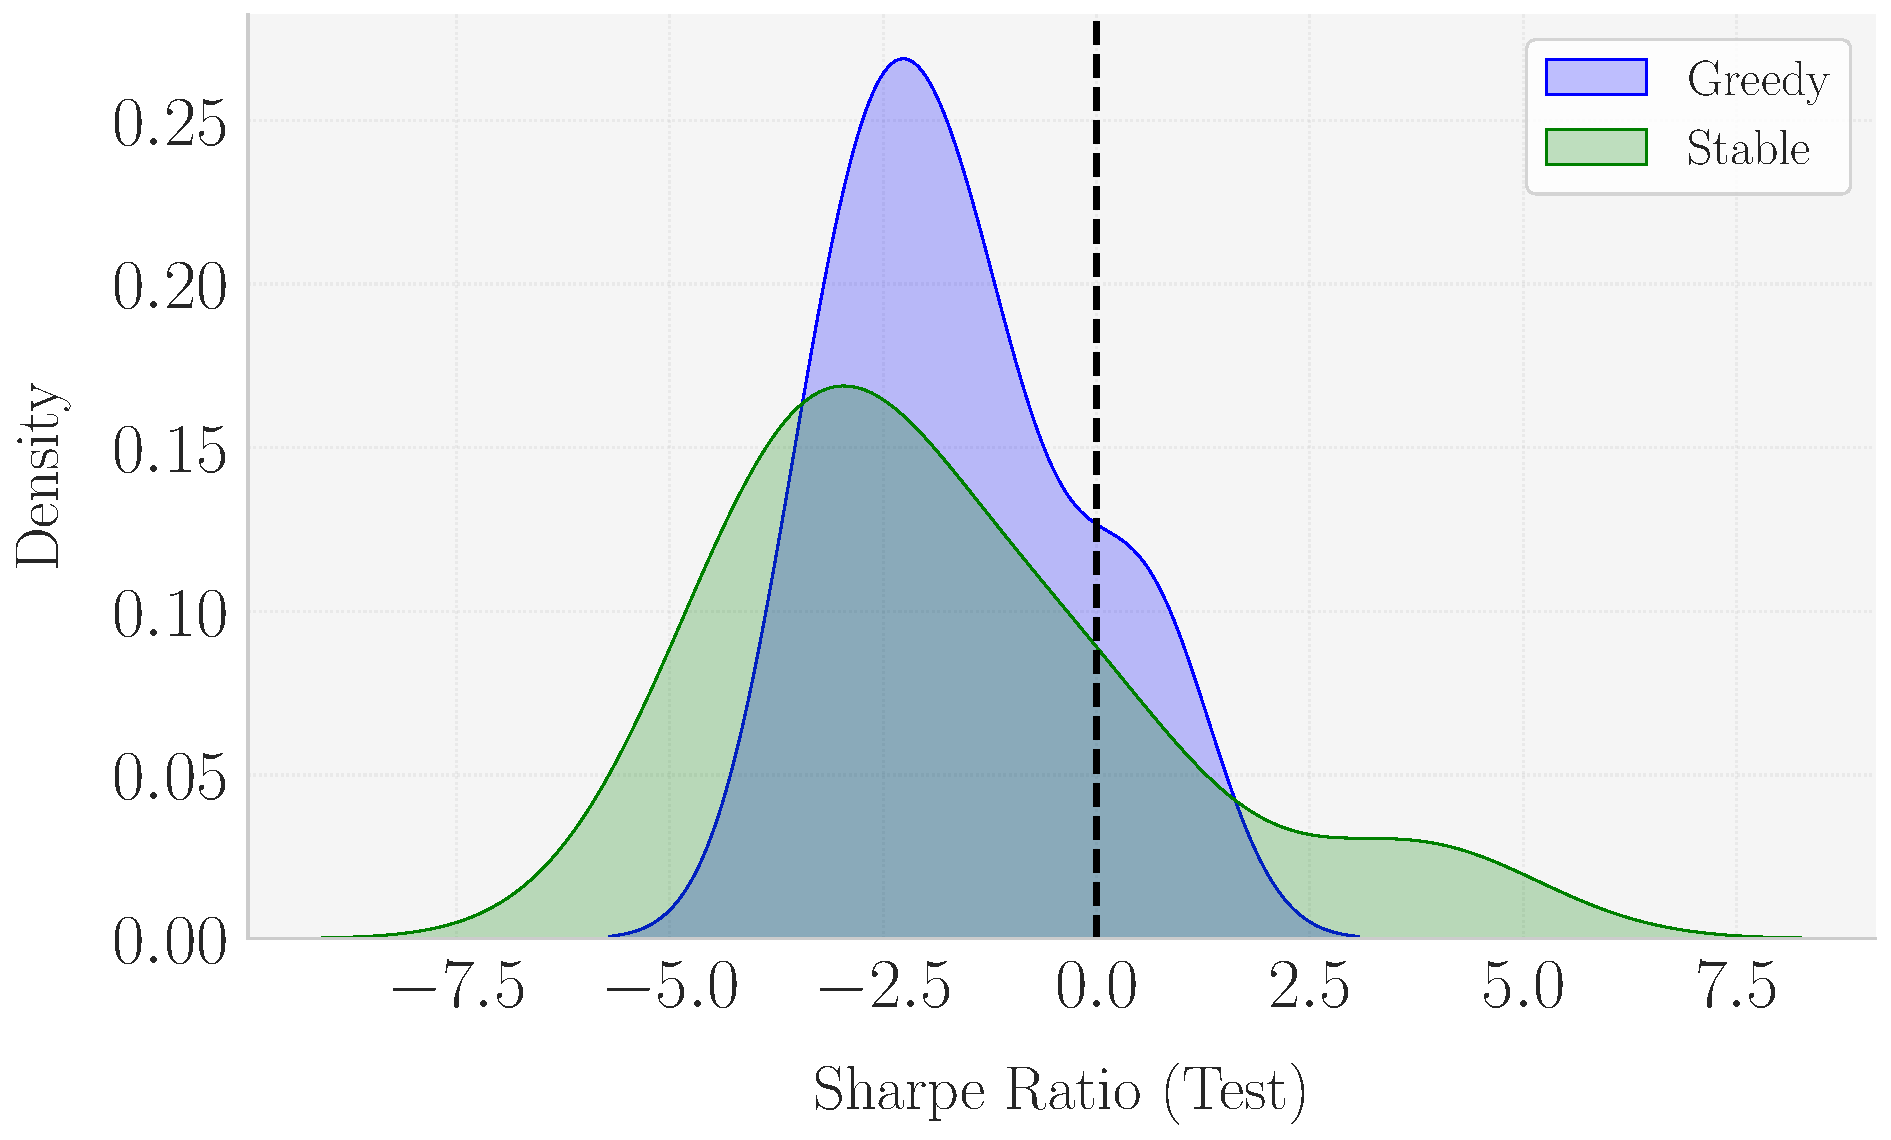
\includegraphics[width=\textwidth]{fig_9a_KMeans_Distr_L(SR-Test).pdf}
%    \caption{\textbf{KMeans}: Distribution of $SR^{\mathcal P^{test}}(L)$}
    \label{fig:KMeans_Robustness_L_Distr}
  \end{subfigure}
  \hspace{0.05\textwidth} % Add horizontal space between the subfigures
  \begin{subfigure}[b]{0.44\textwidth}
    \centering
    \caption{\textbf{KMeans}: Series of $SR^{\mathcal P^{test}}(L)$}
    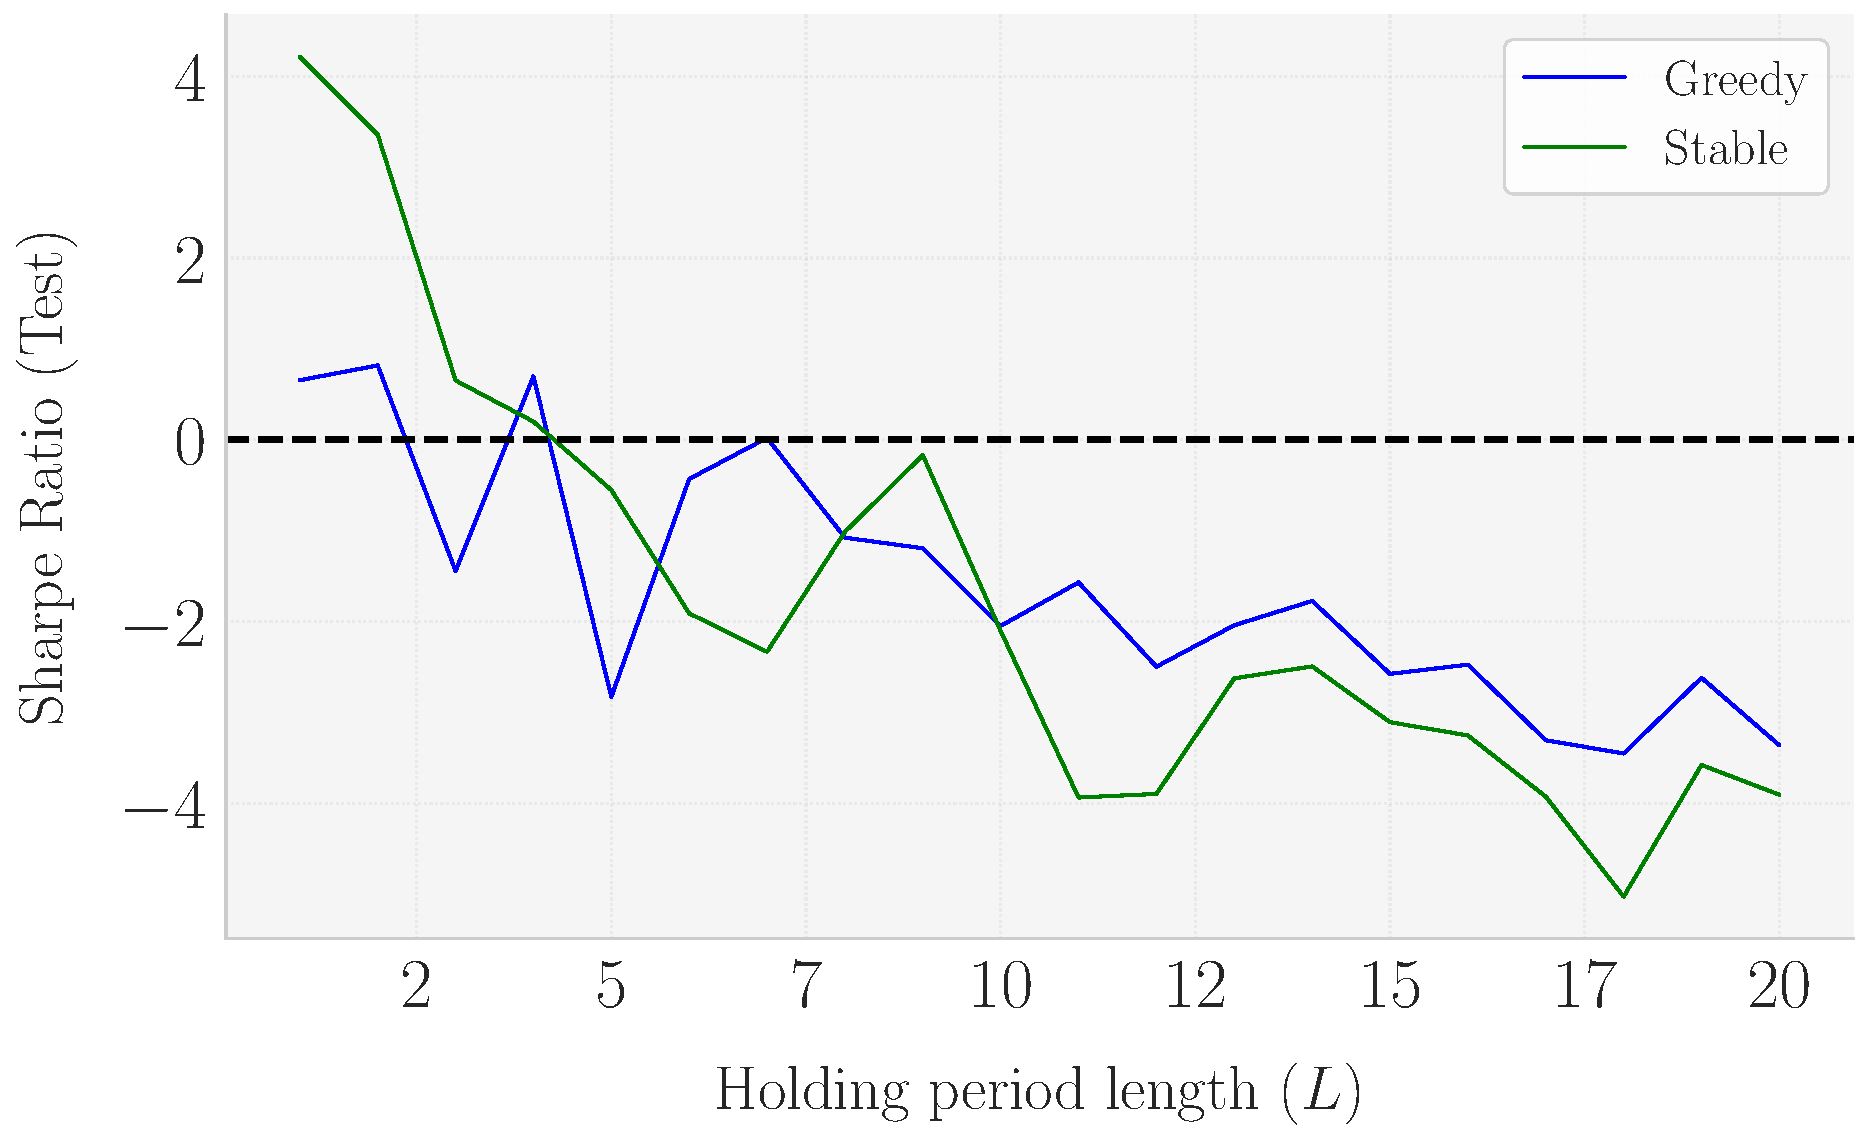
\includegraphics[width=\textwidth]{fig_9b_KMeans_SR-Test_vs_L.pdf}
%    \caption{\textbf{KMeans}: Series of $SR^{\mathcal P^{test}}(L)$}
    \label{fig:KMeans_Robustness_L_Series}
  \end{subfigure}
  
  \bx 
      \begin{subfigure}[b]{0.44\textwidth}
    \centering
    \caption{\textbf{LLM}: Distribution of $SR^{\mathcal P^{test}}(L)$}
    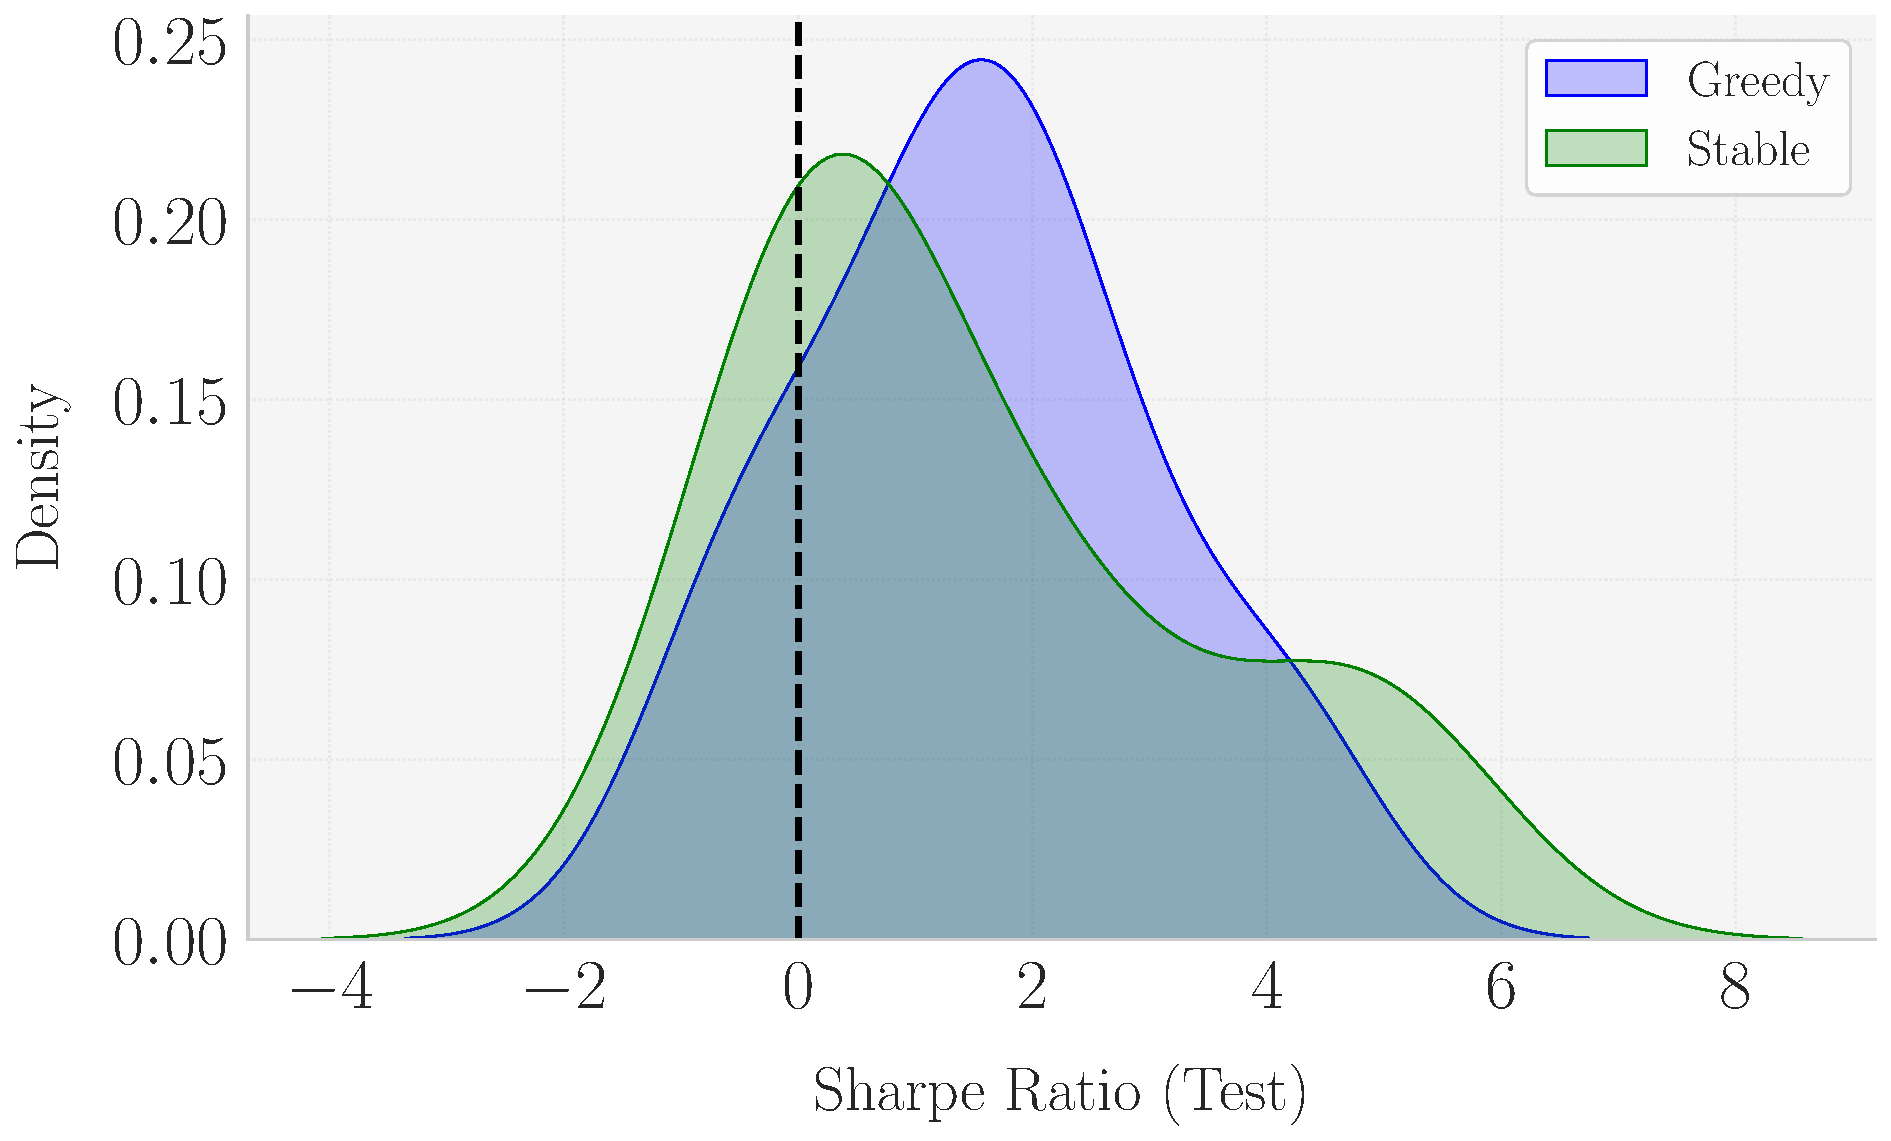
\includegraphics[width=\textwidth]{fig_9c_LLAMA_Distr_L(SR-Test).pdf}
%    \caption{\textbf{LLM}: Distribution of $SR^{\mathcal P^{test}}(L)$}
    \label{fig:LLM_Robustness_L_Distr}
  \end{subfigure}
  \hspace{0.05\textwidth} % Add horizontal space between the subfigures
  \begin{subfigure}[b]{0.44\textwidth}
    \centering
    \caption{\textbf{LLM}: Series of $SR^{\mathcal P^{test}}(L)$}
    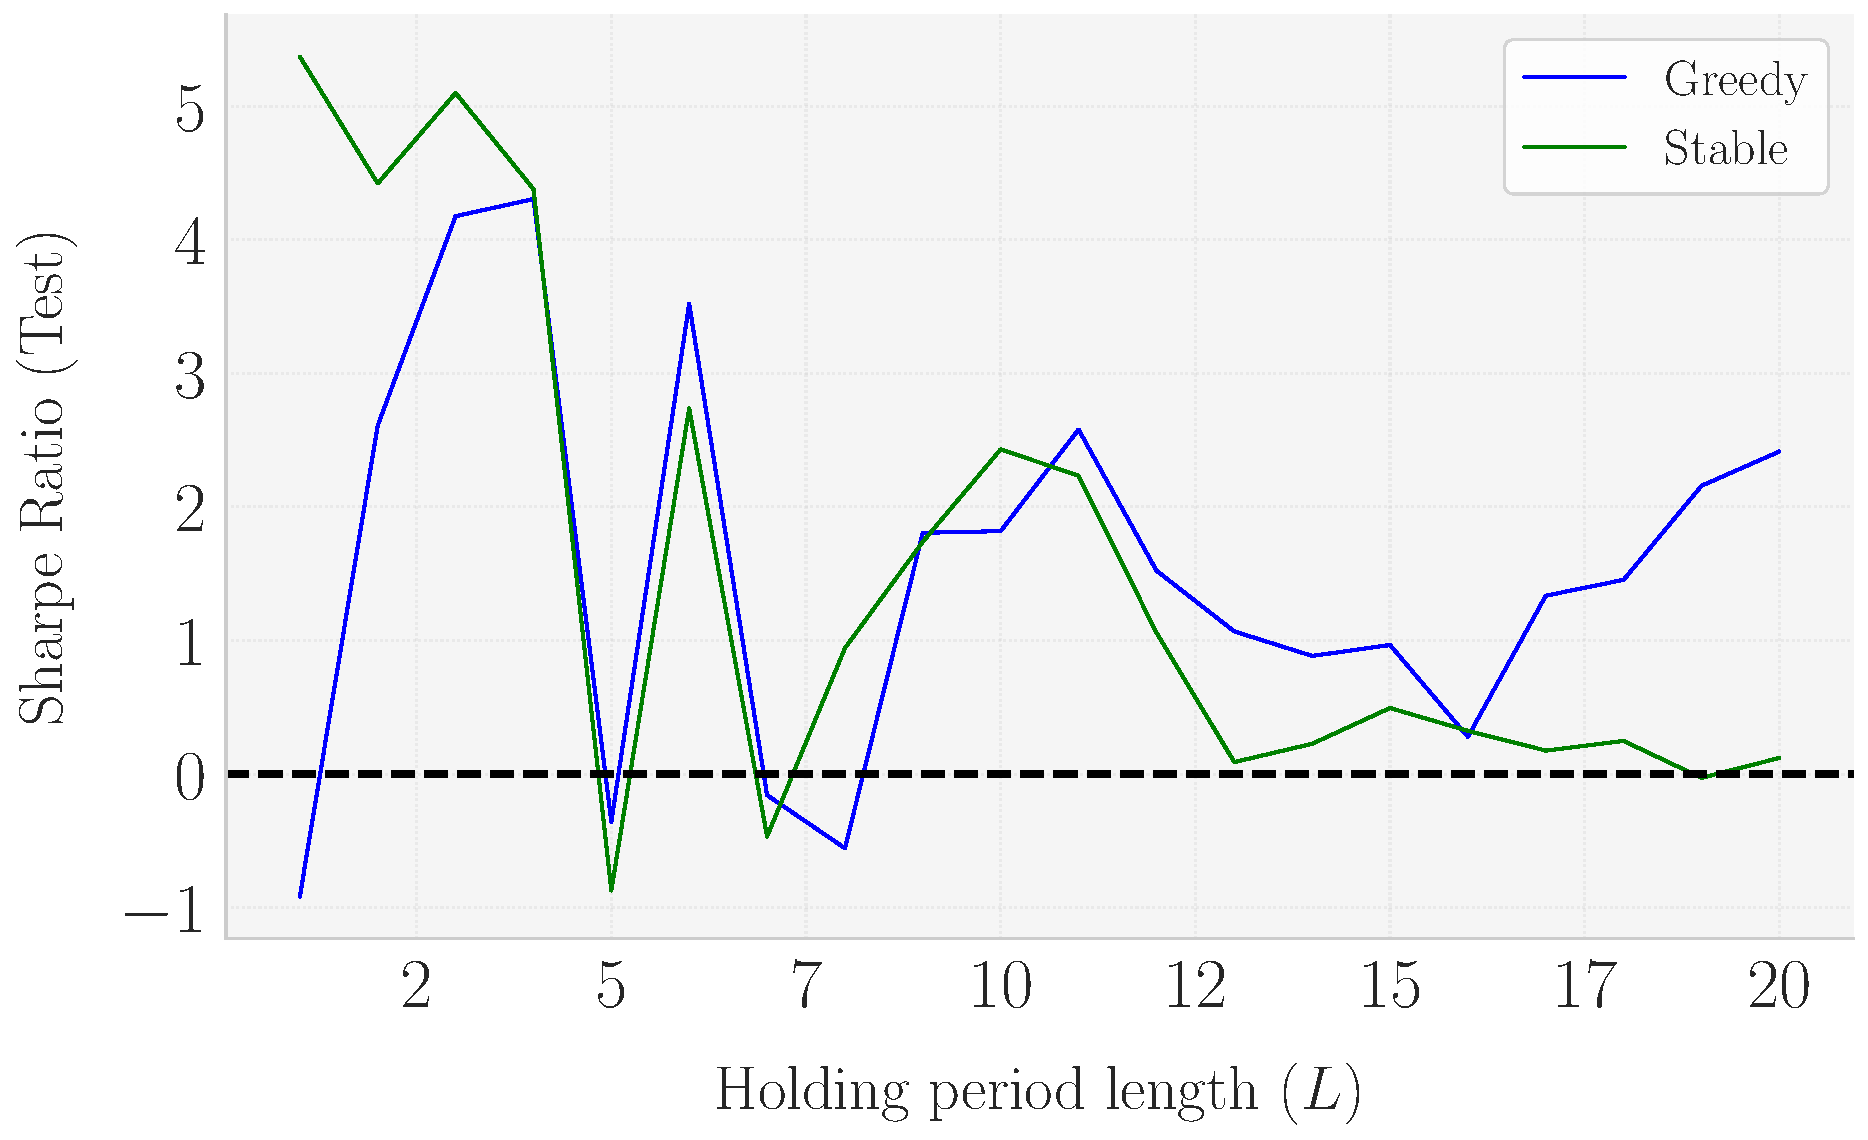
\includegraphics[width=\textwidth]{fig_9d_LLAMA_SR-Test_vs_L.pdf}
%    \caption{\textbf{LLM}: Series of $SR^{\mathcal P^{test}}(L)$}
    \label{fig:LLM_Robustness_L_Series}
  \end{subfigure}
\label{fig:LLM_Robustness_L}
\mx 
\subcaption*{\textit{Note: This figure examines the sensitivity of the Sharpe Ratios ($SR^{\mathcal P^{test}}$) of the test portfolio to changes in the holding window length ($L$), with $\theta$ fixed at $\integer{0.5k}$. Panels \textsc{(a)} and \textsc{(b)} display the distribution and time series of $SR^{\mathcal P^{test}}(L)$ for KMeans clustering, respectively, while Panels \textsc{(c)} and \textsc{(d)} present the same for the LLM-based clustering. The left-hand panels show the skewness of the distributions: KMeans clustering results in a left-skewed distribution of Sharpe Ratios, whereas the LLM-based approach yields a right-skewed distribution, indicating higher profitability. The right-hand panels highlight that KMeans clustering only produces positive Sharpe Ratios for very short holding periods, whereas the LLM-based clustering shows more consistent positive performance across a wider range of $L$ values, though with some variability.}}
\end{figure}
%----------------------------------------------------

From \cref{fig:KMeans_Robustness_L_Distr} it follows that KMeans clustering produces a distribution that is clearly left-skewed, while the distribution of $SR^{\mathcal P ^{test}}$ for LLM clustering is clearly right-skewed (\cref{fig:LLM_Robustness_L_Distr}). This confirms the fact that LLM clustering generates Sharpe Ratios that are statistically higher than those generated by KMeans. The plots in the right-hand-side substantiate this observation: KMeans is only able to produce positive $SR^{\mathcal P ^{test}}$ for really short holding window lengths (\cref{fig:KMeans_Robustness_L_Series}), while LLM clustering, although not always stable, is, in general, able to produce positive Sharpe Ratios more consistently over the grid (\cref{fig:LLM_Robustness_L_Series}).

\mx 
We then turn to analyze the sensitivity of $SR^{\mathcal P^{test}}$ to different values for the upper bound on the number of traded clusters ($\theta$). Now we fix $L=4$ and define a grid $\b \theta$, from where we can obtain $\{SR^{\mathcal P^{test}}(\theta)\}_{\theta\in{\b\theta}}$. 


%----------------------------------------------------
\inserthere{fig:Robustness_theta}
\begin{figure}[H]
  \centering
  \caption{Sensitivity of $SR^{\mathcal P^{test}}$ to the upper bound on the number of traded clusters on each side ($\theta$)}
    \begin{subfigure}[b]{0.46\textwidth}
    \centering
    \caption{\textbf{KMeans}: Distribution of $SR^{\mathcal P^{test}}(\theta)$}
    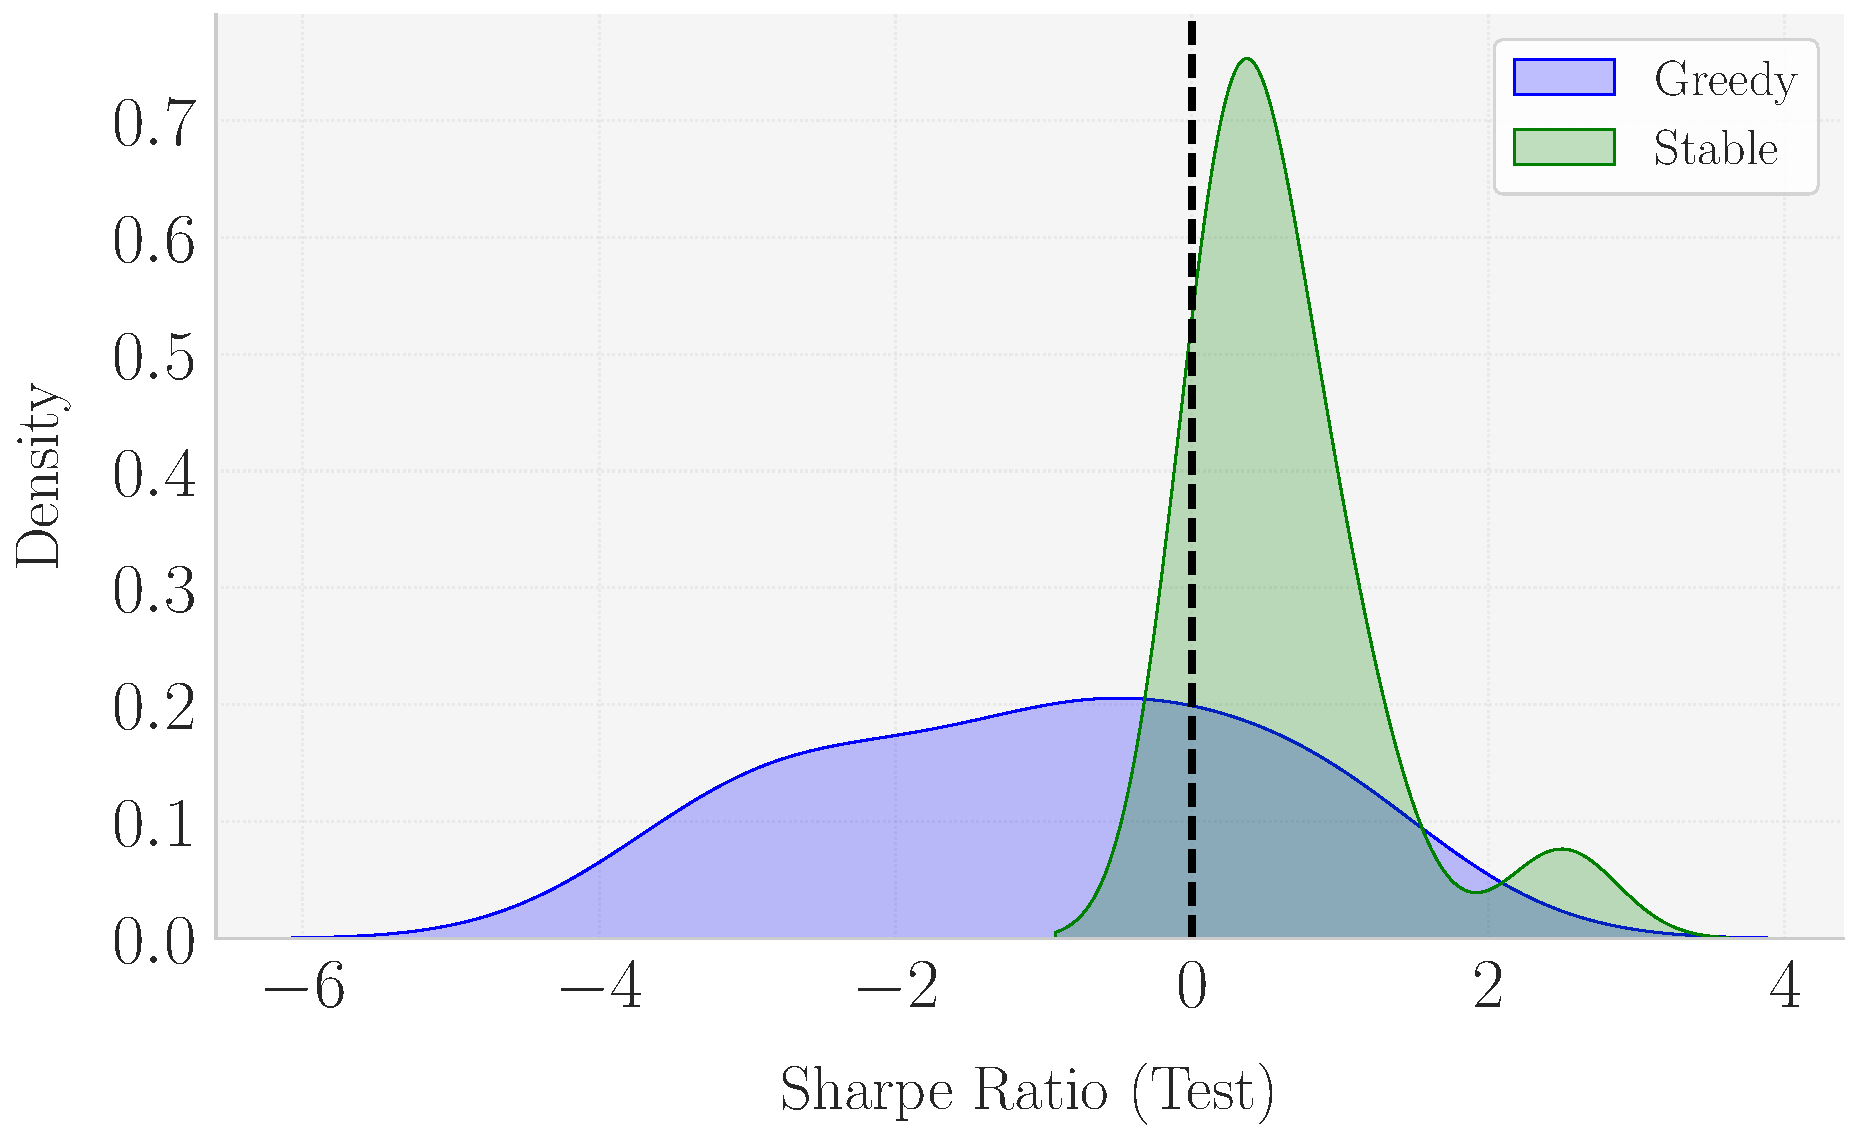
\includegraphics[width=\textwidth]{fig_10a_KMeans_Distr_theta(SR-Test).pdf}
%    \caption{\textbf{KMeans}: Distribution of $SR^{\mathcal P^{test}}(\theta)$}
    \label{fig:KMeans_Robustness_theta_Distr}
  \end{subfigure}
  \hspace{0.05\textwidth} % Add horizontal space between the subfigures
  \begin{subfigure}[b]{0.46\textwidth}
    \centering
    \caption{\textbf{KMeans}: Series of $SR^{\mathcal P^{test}}(\theta)$}
    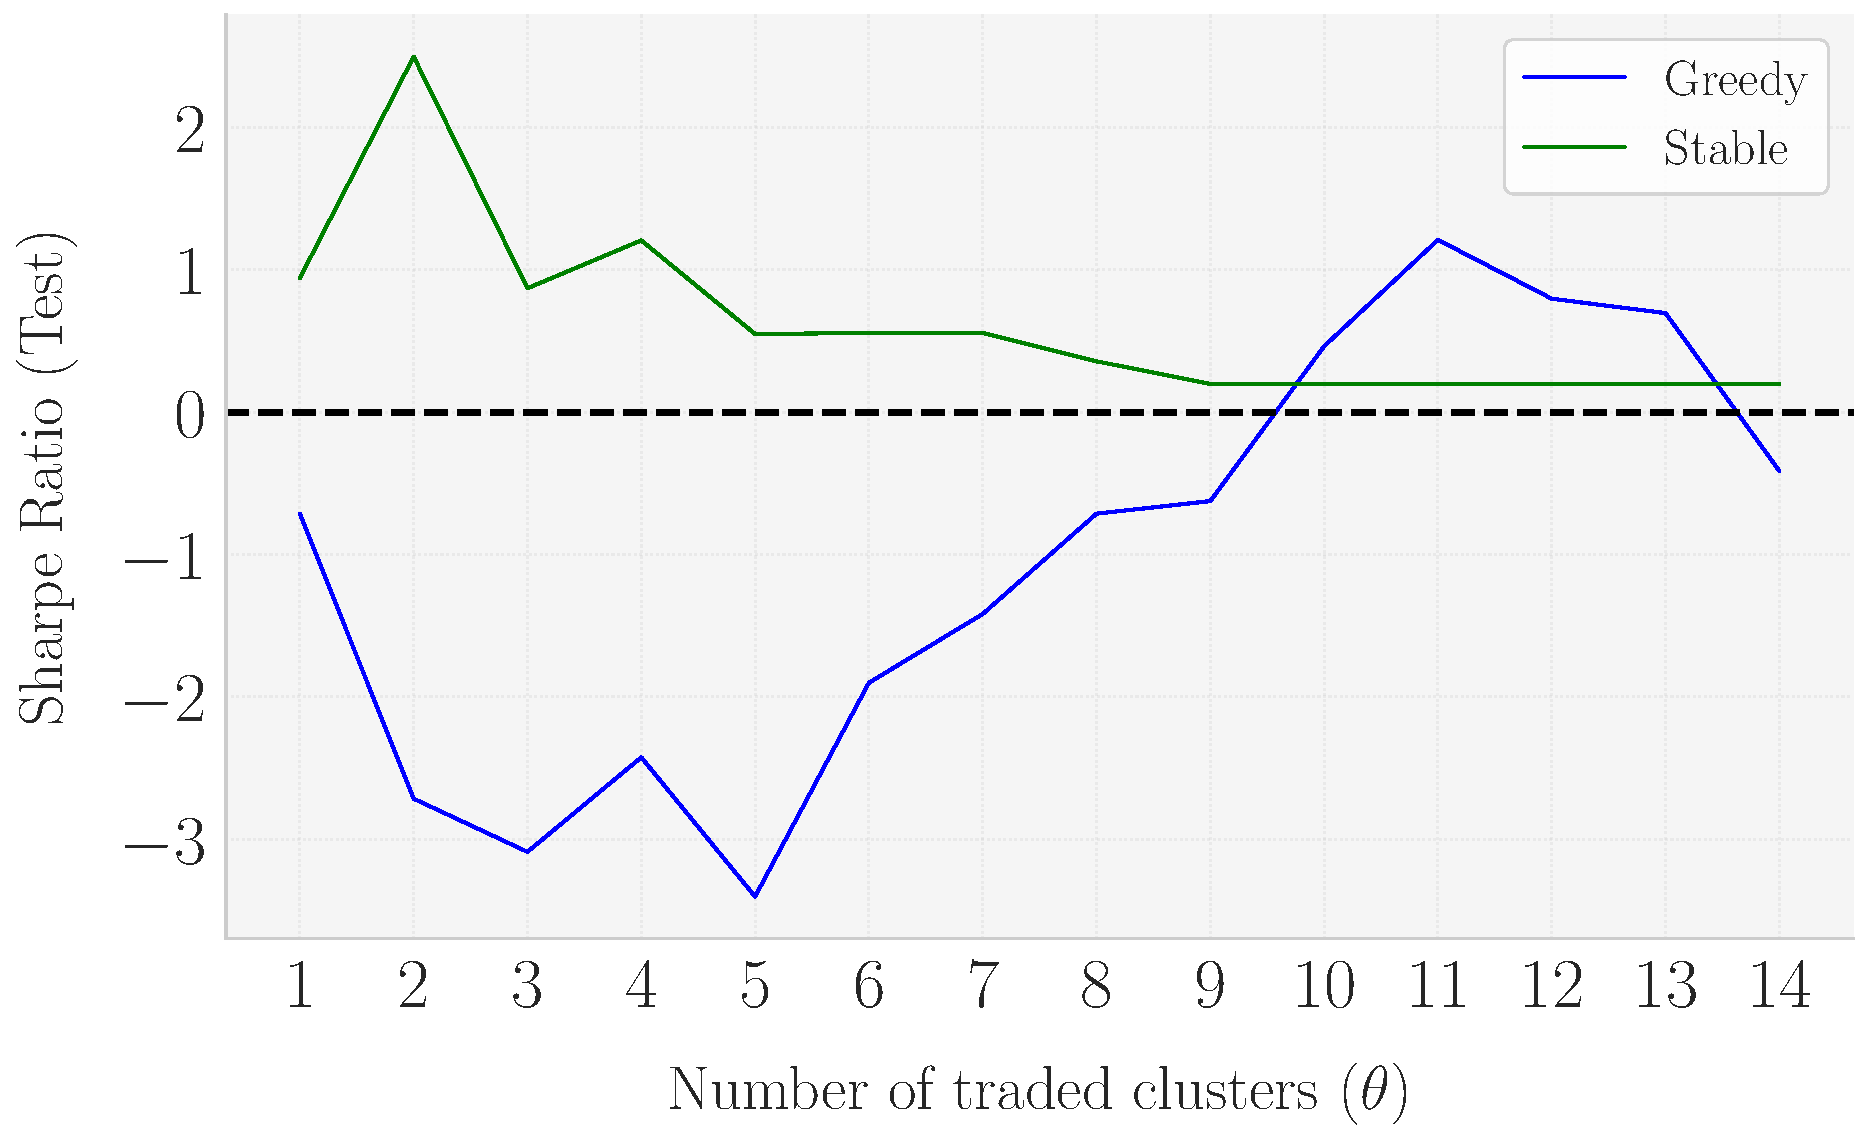
\includegraphics[width=\textwidth]{fig_10b_KMeans_SR-Test_vs_theta.pdf}
%    \caption{\textbf{KMeans}: Series of $SR^{\mathcal P^{test}}(\theta)$}
    \label{fig:KMeans_Robustness_theta_Series}
  \end{subfigure}
  
  \bx 
      \begin{subfigure}[b]{0.46\textwidth}
    \centering
    \caption{\textbf{LLM}: Distribution of $SR^{\mathcal P^{test}}(\theta)$} 
    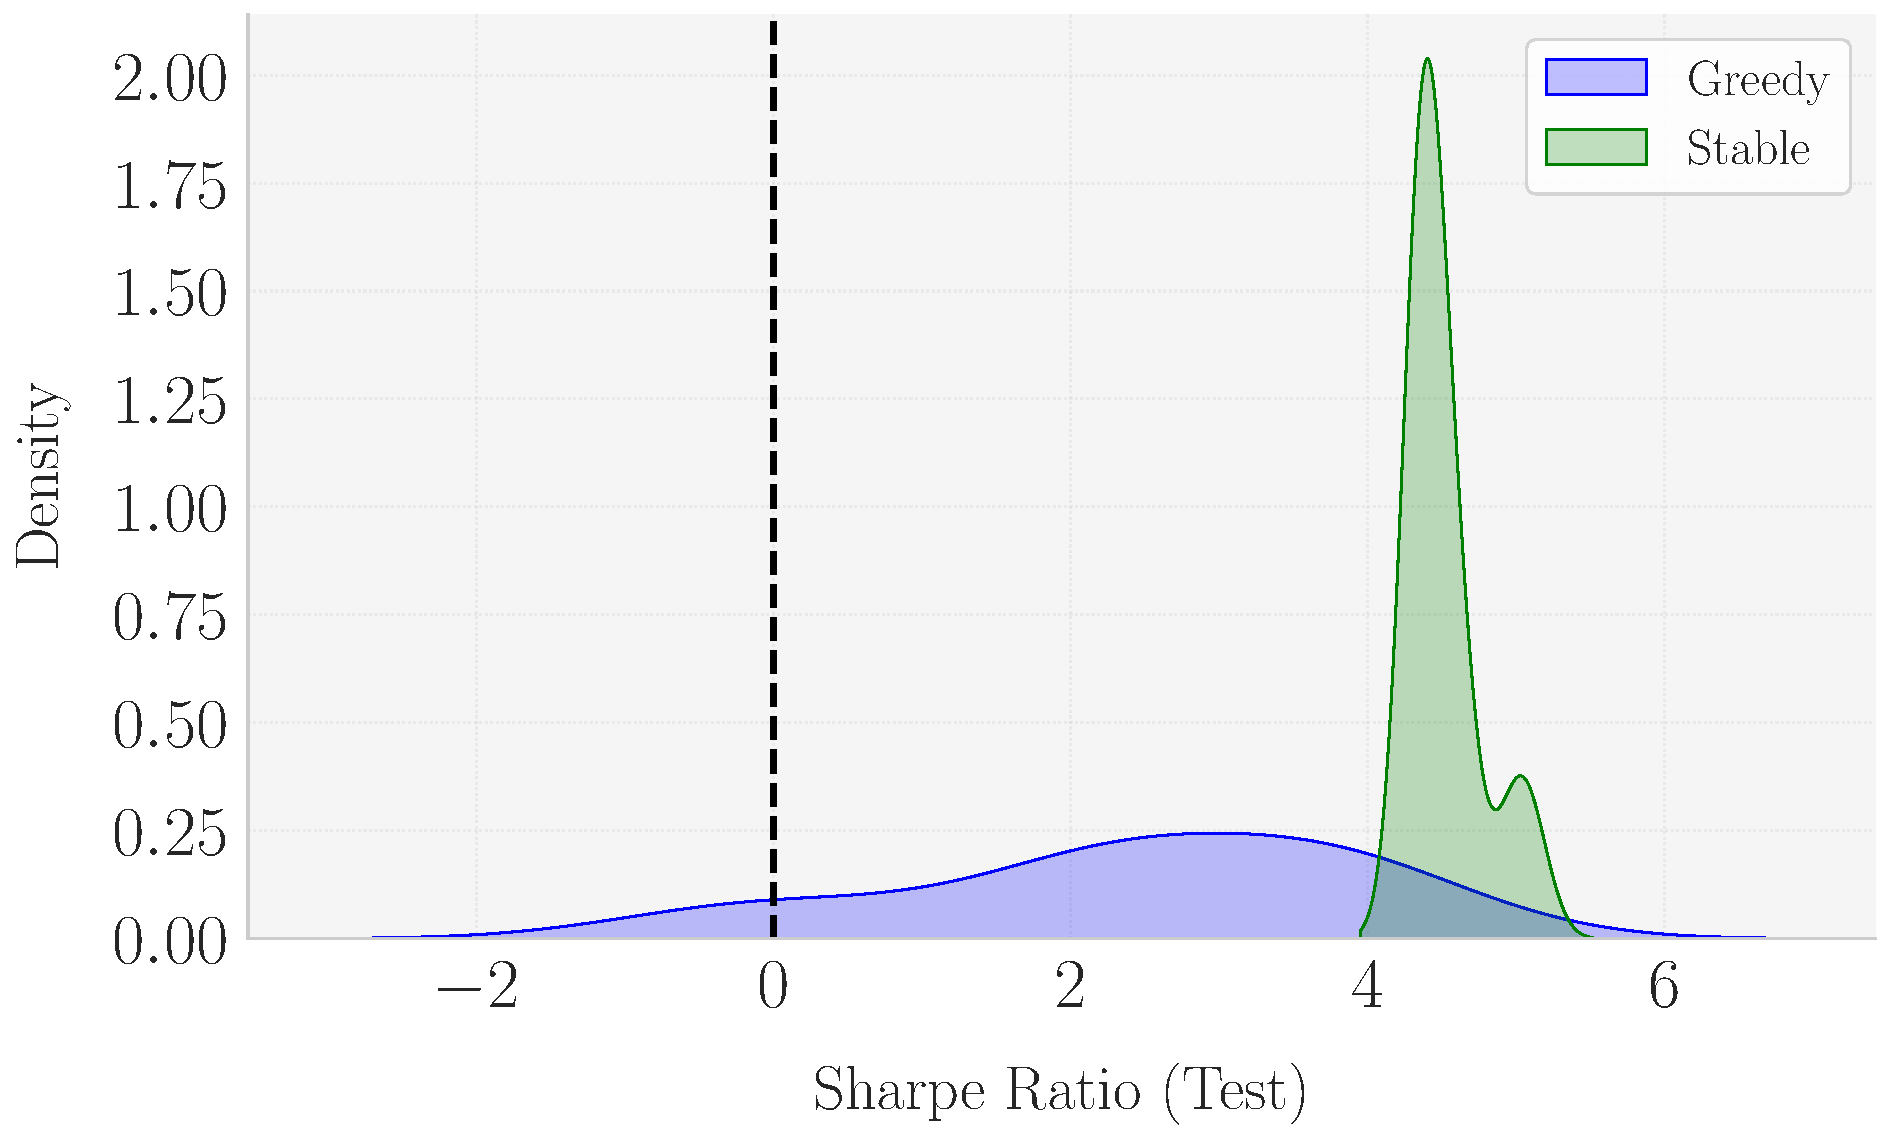
\includegraphics[width=\textwidth]{fig_10c_LLAMA_Distr_theta(SR-Test).pdf}
%    \caption{\textbf{LLM}: Distribution of $SR^{\mathcal P^{test}}(\theta)$}
    \label{fig:LLM_Robustness_theta_Distr}
  \end{subfigure}
  \hspace{0.05\textwidth} % Add horizontal space between the subfigures
  \begin{subfigure}[b]{0.46\textwidth}
    \centering
    \caption{\textbf{LLM}: Series of $SR^{\mathcal P^{test}}(\theta)$} 
    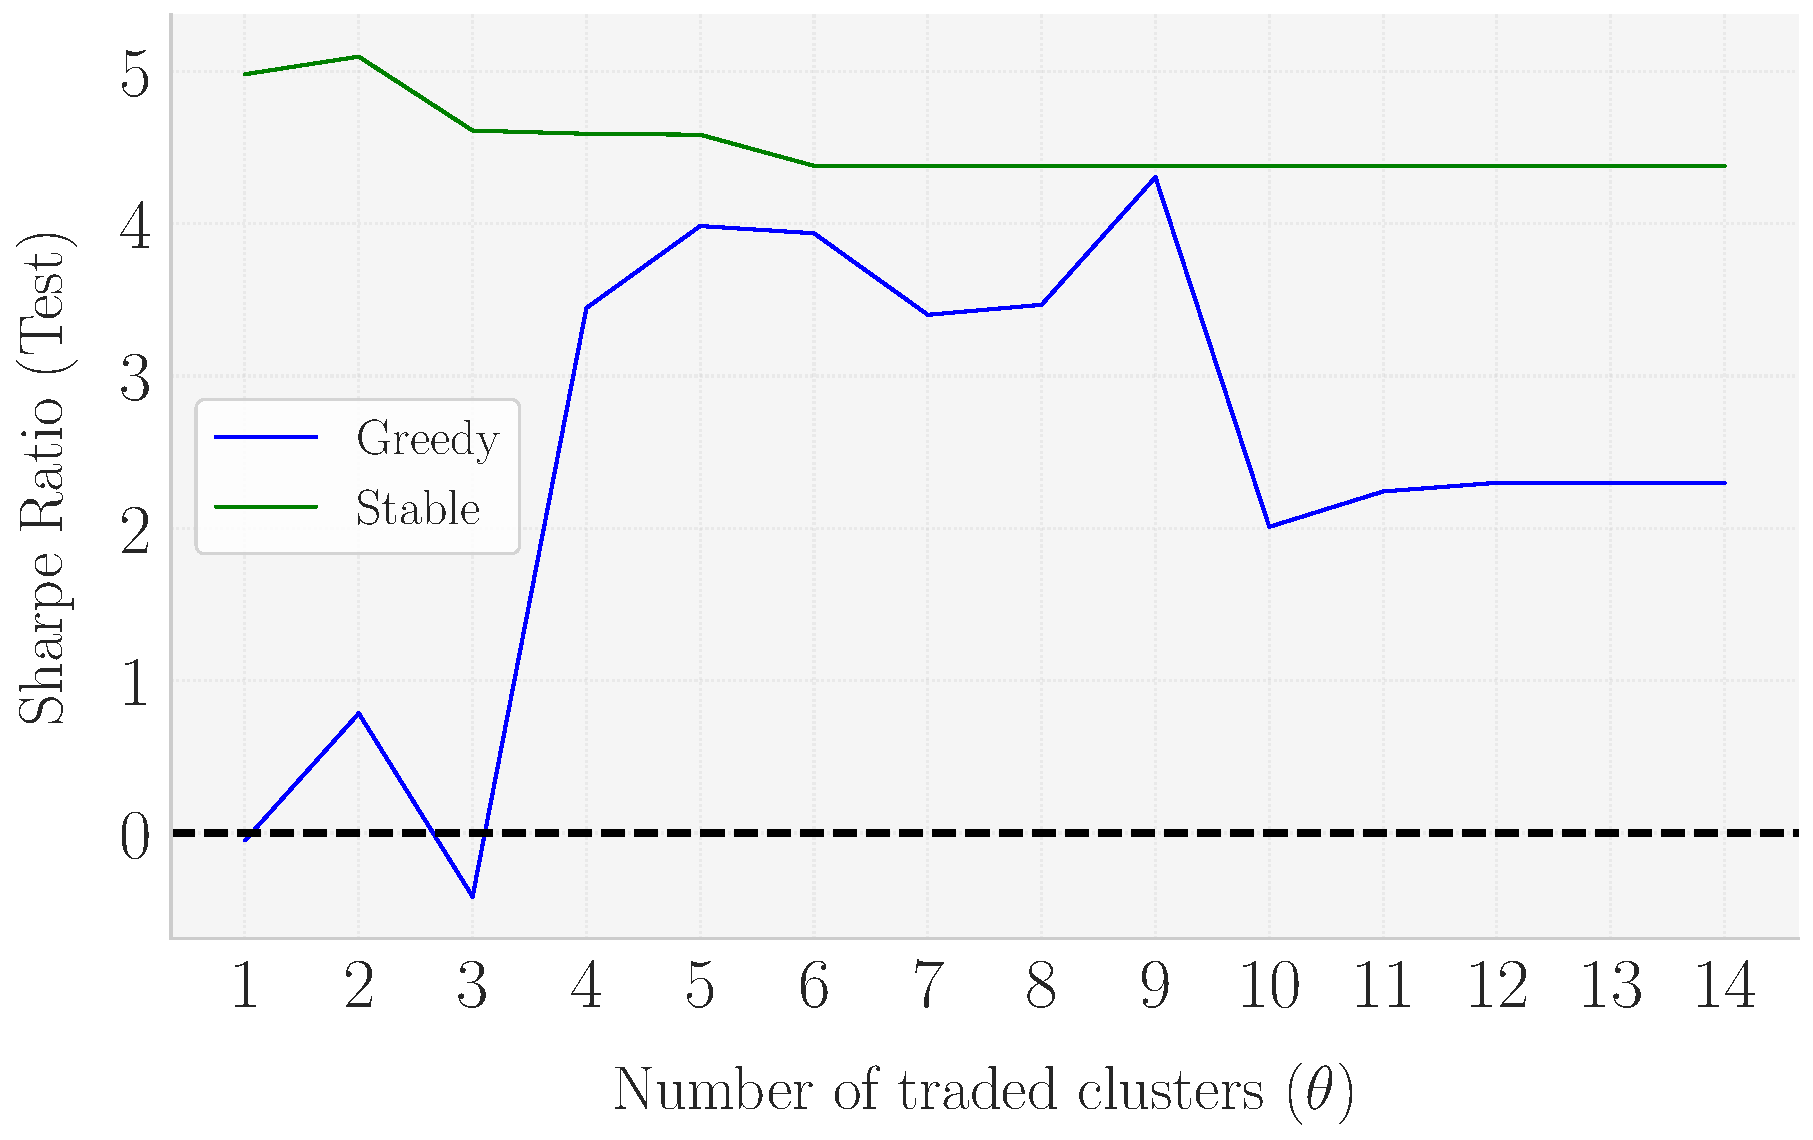
\includegraphics[width=\textwidth]{fig_10d_LLAMA_SR-Test_vs_theta.pdf}
%    \caption{\textbf{LLM}: Series of $SR^{\mathcal P^{test}}(\theta)$}
    \label{fig:LLM_Robustness_theta_Series}
  \end{subfigure}

\mx 
\subcaption*{\textit{Note: This figure displays the sensitivity of the Sharpe Ratios ($SR^{\mathcal P^{test}}$) to variations in the upper bound on the number of traded clusters ($\theta$), with $L$ fixed at 4. Panels \textsc{(a)} and \textsc{(b)} show the distribution and series of $SR^{\mathcal P^{test}}(\theta)$ for KMeans clustering, respectively, while Panels \textsc{(c)} and \textsc{(d)} illustrate the same for LLM-based clustering. For KMeans, the results are mixed: the \textit{Stable} algorithm generates positive Sharpe Ratios for low $\theta$ values, whereas the \textit{Greedy} algorithm performs better with high $\theta$ values, indicating sensitivity and instability. In contrast, the LLM-based clustering shows a more consistent pattern, with a concentration of positive Sharpe Ratios across a broader range of $\theta$ values, suggesting greater robustness and stability in the trading strategy.}}

\label{fig:Robustness_theta}
\end{figure}
%----------------------------------------------------


The results of this exercise are shown in \cref{fig:Robustness_theta}. As we can see, in \cref{fig:KMeans_Robustness_theta_Distr} the results are mixed for the case of KMeans clustering. Namely, the \textit{Stable} algorithm is able to generate positive Sharpe Ratios but the \textit{Greedy} algorithm struggles to do so. In \cref{fig:KMeans_Robustness_theta_Series} we see what is happening: \textit{Stable} works well with for low values of $\theta$, while \textit{Greedy} only works for high values of $\theta$. This high reliance of the algorithms on specific values of $\theta$ points to the instability of the trading strategy when employing KMeans clustering.

\mx 
On the other hand, \cref{fig:LLM_Robustness_theta_Distr} shows a clear pattern for the case of LLM clustering. Namely, the mass accumulates at high and positive Sharpe Ratios. This observation is further substantiated by \cref{fig:KMeans_Robustness_theta_Series}, which shows that leaving aside the fact that the greedy algorithm does bad for really low values of $\theta$ (i.e.: $\theta\leq 3$), in general, the trading strategy is now able to produce high, positive and stable Sharpe Ratios across different values of $\theta$.  

\mx
All in all, our results are robust to hyperparameter variability, showing that LLM clustering consistently beats a strategy based on clustering embeddings with KMeans. 


%%%%%%%%%%%%%%% TRADING INTENSITY %%%%%%%%%%%%%%%%%%%%%
%\section{Trading Intensity}
The extraordinary performance of our proposed LLM-based methodology warrants a careful examination of its implementation costs and practical viability. While our primary objective has been to develop a framework that better captures the economic content of news articles and their subsequent market impact, the practical implementation of such strategies necessarily involves trading frictions that could affect their real-world efficacy. In this section, we analyze the trading intensity patterns of both methodologies to provide a more complete assessment of their relative merits and to understand how transaction costs might influence their comparative advantages.
We begin by examining the temporal evolution of open positions for both approaches, which provides insights into their underlying trading dynamics and stability characteristics. This analysis is followed by detailed trading intensity metrics and concludes with a reassessment of portfolio statistics after accounting for transaction costs.

%The results from the trading strategy are really good, almost too good to be true. 
%
%As we already said, this is a paper whose goal is to better understand the incorporation of information into the market, so our focus was preeminently in developing a methodology that is able to anticipate the markets. In the process, we ignored the implications of the trading intensity of the strategy and focused only on trying to see if providing economic structure when parsing news articles did really provide improved insights into predicting market reactionsto news. 
%
%In this section, we shed light into the trading intensity of the trading strategy to see how our conclusions change as we consider realistic implications such as trading costs into the analysis. First, we will plot the number of open positions per day implied by each algorithm. 

%----------------------------------------------------
\inserthere{fig:open_positions_comparison}

\begin{figure}[htbp]
\caption{Evolution of Open Positions: KMeans vs LLM Clustering}
\label{fig:open_positions_comparison}

% Panel A: KMeans
\begin{subfigure}{\textwidth}
\caption{Panel A: KMeans Clustering}
\centering
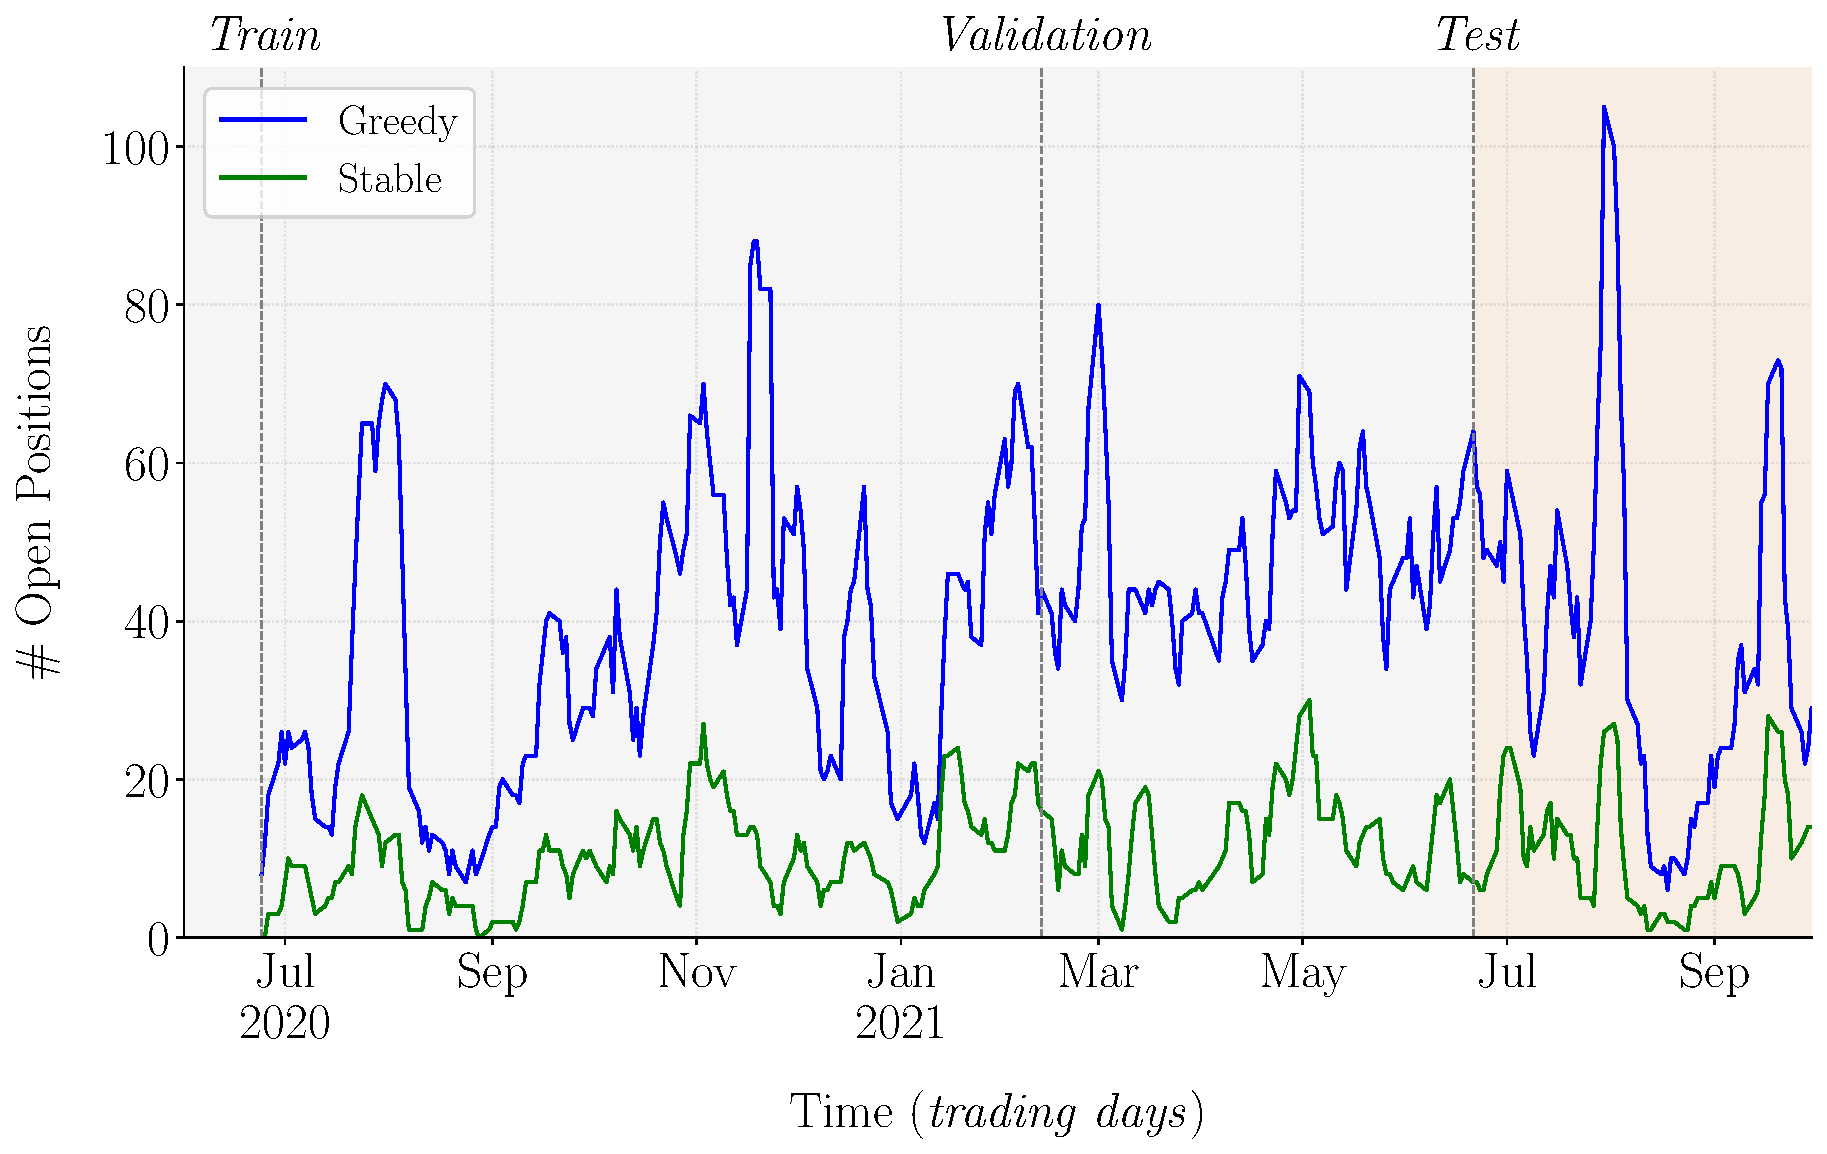
\includegraphics[scale=0.45]{fig_KMeans_Open_Positions.pdf}
\end{subfigure}

\vspace{0.7cm}

% Panel B: LLM
\begin{subfigure}{\textwidth}
\caption{Panel B: LLM Clustering}
\centering
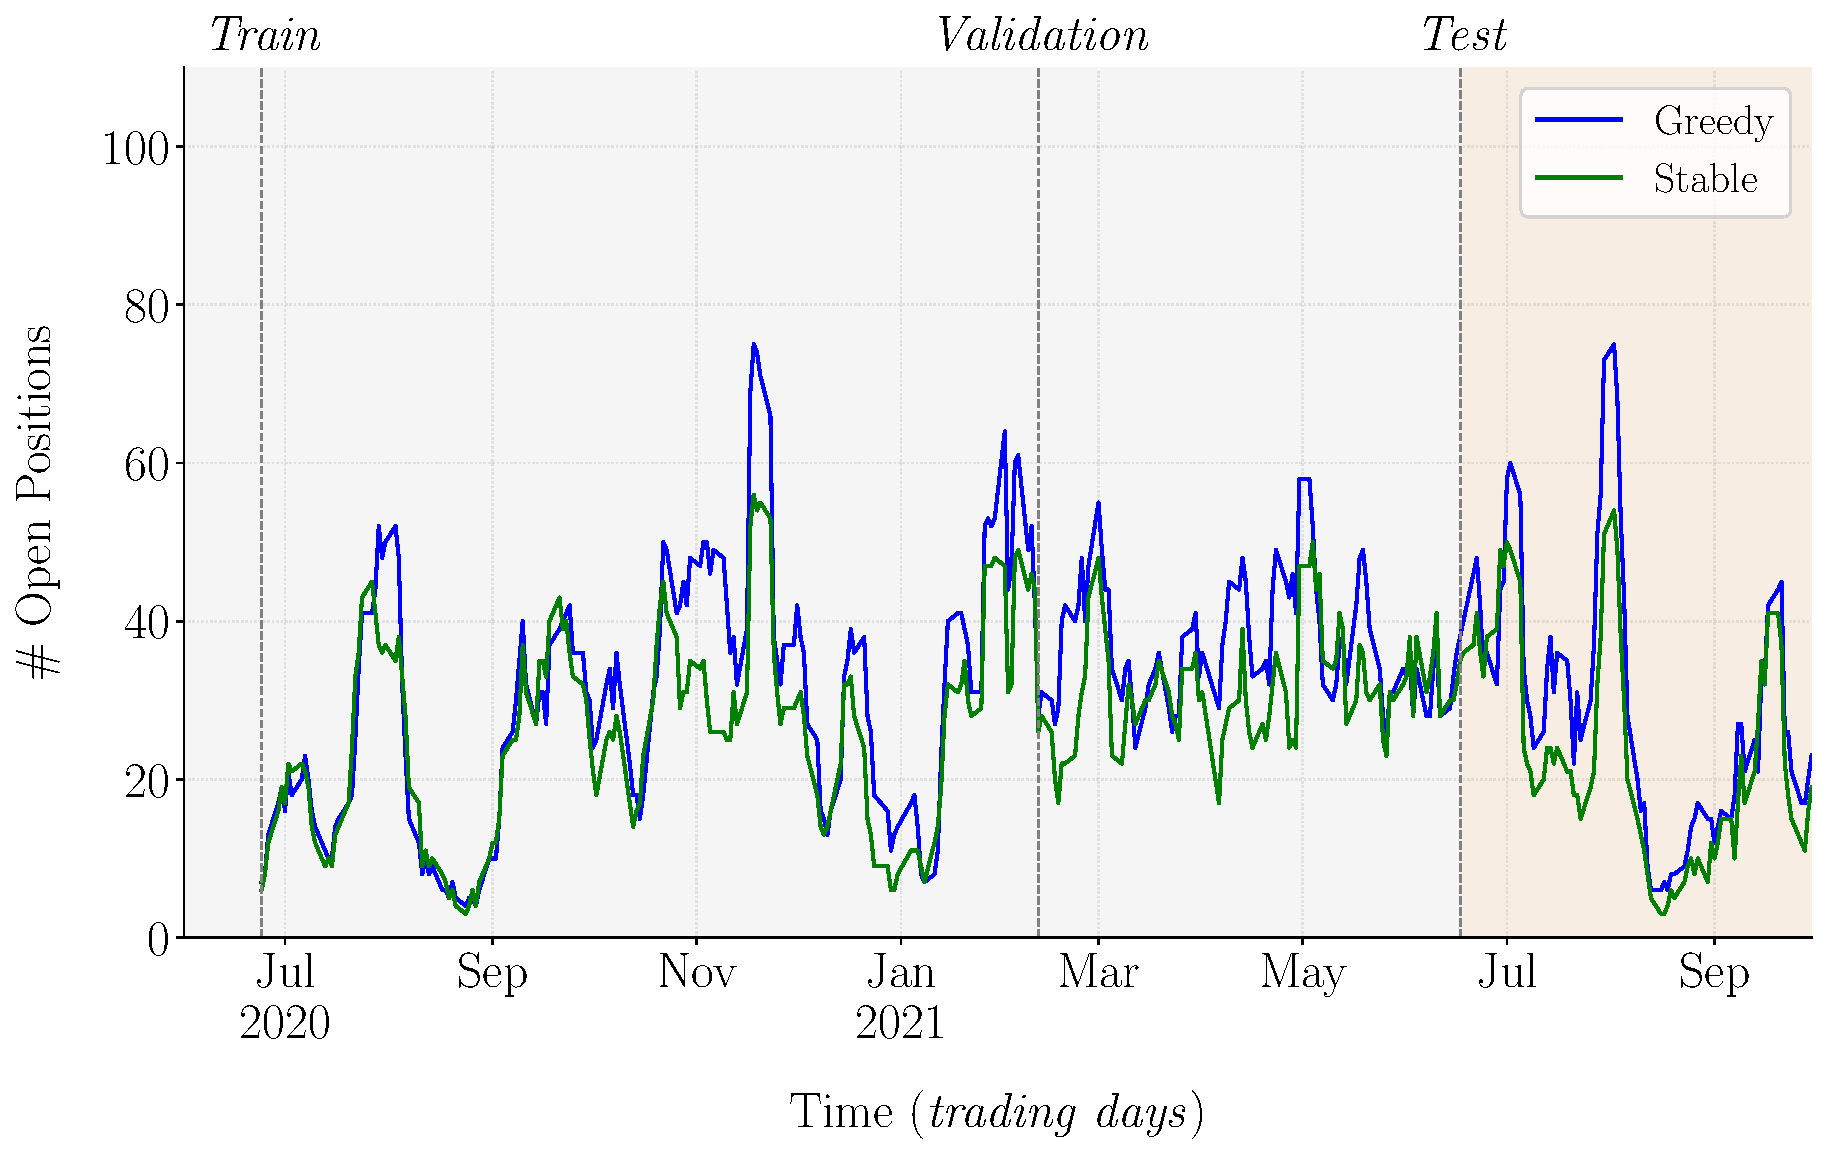
\includegraphics[scale=0.45]{fig_LLAMA_Open_Positions.pdf}
\end{subfigure}

\vspace{0.2cm}
\begin{minipage}{\textwidth}
\setlength{\parindent}{0pt}
{\footnotesize\textit{Note: 
This figure shows the daily evolution of the number of open positions for both Greedy (blue) and Stable (green) algorithms across different data splits (Train, Validation, Test) using KMeans clustering (Panel A) and LLM clustering (Panel B). The time period spans from July 2020 to September 2021. Vertical dashed lines separate the different data splits. The Greedy algorithm selects clusters that maximize (minimize) the cluster-average-$SR$ for long (short) positions, while the Stable algorithm minimizes the rank difference between training and validation rankings. The number of traded clusters is $\theta = 0.5k=13$ for KMeans ($k^*=26$ clusters) and $\theta = 0.5k=10$ for LLM ($k^*=20$ clusters).
}}
\end{minipage}
\end{figure}
%----------------------------------------------------

The temporal evolution of open positions reveals fundamental differences in the stability and reliability of trading signals generated by KMeans versus LLM-based clustering approaches. The KMeans implementation exhibits pronounced volatility in position management, particularly evident in the Greedy algorithm's behavior, which shows extreme fluctuations ranging from 6 to 105 positions. This erratic pattern suggests that KMeans-detected clusters are highly sensitive to market noise and potentially capture transient correlations rather than fundamental relationships. The substantial divergence between Greedy and Stable algorithms under KMeans further underscores the method's instability, as even minor variations in cluster selection criteria lead to dramatically different trading decisions.
In stark contrast, the LLM-based approach demonstrates remarkably more coherent and stable position management. Both Greedy and Stable algorithms maintain more closely aligned position counts, typically ranging between 20 and 75 positions, with highly correlated temporal movements. This convergence in behavior between algorithms suggests that LLM-identified clusters capture more fundamental and persistent market relationships. Particularly telling is the test period performance, where KMeans exhibits increased position volatility and extreme spikes, while the LLM approach maintains consistent position patterns across both algorithms. This stability in the out-of-sample period provides strong evidence that LLM-derived signals, grounded in economic analysis of firm-specific shocks, generalize more effectively to unseen data.

%----------------------------------------------------
\inserthere{tab:trading_intensity_comparison}

\begin{table}[htbp] 
\caption{Trading Intensity Analysis: Model Comparison} 
\centering 
\label{tab:trading_intensity_comparison}

\begin{subtable}{\textwidth}
\caption{Panel A: KMeans}
\centering 
{\small
\begin{tabular}{lcccccccccc}
\toprule
\textbf{Split} & \textbf{Algorithm} & \multicolumn{4}{c}{\textbf{\# Open Positions}} & \multicolumn{2}{c}{\textbf{Trading Activity (\%)}} & \multicolumn{2}{c}{\textbf{Trading Costs (\%)}} \\
\cmidrule(lr{0.6em}){3-6} \cmidrule(lr{0.6em}){7-8} \cmidrule(lr{0.6em}){9-10}
& & \textbf{Avg}. & \textbf{Std}. & \textbf{Max} & \textbf{Min} & \textbf{Turnover} & \textbf{Changes/Pos.} & \textbf{Cost} & \textbf{Active} \\
\midrule
\multirow{2}{*}{All} & \textit{Greedy} & 40.1 & 18.59 & 105 & 6 & 32.03 & 0.798 & 0.0961 & 100.0 \\
 & \textit{Stable} & 10.77 & 6.41 & 30 & 0 & 34.75 & 3.228 & 0.1042 & 99.1 \\
\midrule
\multirow{2}{*}{Train} & \textit{Greedy} & 36.4 & 19.33 & 88 & 7 & 30.59 & 0.840 & 0.0918 & 100.0 \\
 & \textit{Stable} & 9.89 & 5.93 & 27 & 0 & 33.73 & 3.412 & 0.1012 & 98.2 \\
\midrule
\multirow{2}{*}{Validation} & \textit{Greedy} & 48.4 & 10.00 & 80 & 30 & 31.39 & 0.649 & 0.0942 & 100.0 \\
 & \textit{Stable} & 12.34 & 6.05 & 30 & 1 & 33.42 & 2.708 & 0.1003 & 100.0 \\
\midrule
\multirow{2}{*}{Test} & \textit{Greedy} & 38.8 & 21.74 & 105 & 6 & 35.86 & 0.925 & 0.1076 & 100.0 \\
 & \textit{Stable} & 10.84 & 7.47 & 28 & 1 & 39.30 & 3.626 & 0.1179 & 100.0 \\
\bottomrule
\end{tabular}
}
\end{subtable}

\vspace{0.6cm}

\begin{subtable}{\textwidth}
\caption{Panel B: LLM}
\centering
{\small
\begin{tabular}{lcccccccccc}
\toprule
\textbf{Split} & \textbf{Algorithm} & \multicolumn{4}{c}{\textbf{\# Open Positions}} & \multicolumn{2}{c}{\textbf{Trading Activity (\%)}} & \multicolumn{2}{c}{\textbf{Trading Costs (\%)}} \\
\cmidrule(lr{0.6em}){3-6} \cmidrule(lr{0.6em}){7-8} \cmidrule(lr{0.6em}){9-10}
& & \textbf{Avg}. & \textbf{Std}. & \textbf{Max} & \textbf{Min} & \textbf{Turnover} & \textbf{Changes/Pos.} & \textbf{Cost} & \textbf{Active} \\
\midrule
\multirow{2}{*}{All} & \textit{Greedy} & 31.8 & 14.84 & 75 & 4 & 39.21 & 1.234 & 0.1176 & 100.0 \\
 & \textit{Stable} & 26.61 & 12.16 & 56 & 3 & 39.18 & 1.473 & 0.1175 & 100.0 \\
\midrule
\multirow{2}{*}{Train} & \textit{Greedy} & 29.9 & 16.34 & 75 & 4 & 40.42 & 1.351 & 0.1212 & 100.0 \\
 & \textit{Stable} & 25.54 & 12.90 & 56 & 3 & 40.45 & 1.584 & 0.1213 & 100.0 \\
\midrule
\multirow{2}{*}{Validation} & \textit{Greedy} & 37.0 & 7.69 & 58 & 24 & 38.43 & 1.039 & 0.1153 & 100.0 \\
 & \textit{Stable} & 31.38 & 6.82 & 50 & 17 & 37.95 & 1.209 & 0.1138 & 100.0 \\
\midrule
\multirow{2}{*}{Test} & \textit{Greedy} & 29.7 & 16.24 & 75 & 6 & 37.56 & 1.264 & 0.1127 & 100.0 \\
 & \textit{Stable} & 23.43 & 13.71 & 54 & 3 & 37.85 & 1.615 & 0.1135 & 100.0 \\
\bottomrule
\end{tabular}
}
\end{subtable}

\vspace{0.5cm}
\begin{minipage}{\textwidth}
\setlength{\parindent}{0pt}
\small\textit{Note: 
This table presents trading intensity metrics for both Greedy and Stable algorithms across different data splits for two different models: KMeans (Panel A) and LLM (Panel B). 
The metrics are computed at a daily frequency. The `\# Open Positions' columns report position-related statistics: 
`Avg.' shows the mean number of concurrent open positions per day, `Std.' represents their standard deviation, while 
`Max' and `Min' indicate the maximum and minimum number of positions held simultaneously. Under `Trading Activity (\%)', 
`Turnover' is calculated as the sum of absolute changes in position sizes divided by the total portfolio size, expressed 
as a percentage; formally, $Turnover_t = 100 \times (\sum_i |w_{i,t} - w_{i,t-1}|)/(\sum_i |w_{i,t}|)$, where $w_{i,t}$ 
represents the position size in asset $i$ at time $t$. `Changes/Pos.' represents the average number of modifications per 
position per day, computed as the daily turnover divided by the average number of positions, providing insight into how 
actively individual positions are managed. 
The `Trading Costs (\%)' section reports `Cost' as the average daily implementation shortfall (computed as the product of daily turnover and a conservative transaction cost parameter of 30 basis points, representing both direct and indirect trading costs) expressed in percentage terms, while `Active' shows the percentage of trading days with at least one open position.
%
%The `Trading Costs (\%)' section reports `Cost' as the average daily implementation 
%shortfall (computed as the difference between gross and net returns) expressed in percentage terms, while `Active' shows 
%the percentage of trading days with at least one open position. 
All metrics are first computed daily and then averaged over their respective periods, except for Max and Min positions which represent the absolute extremes over each period.
}
\end{minipage}
\end{table}
%----------------------------------------------------

% Analysis of Trading Intensity Metrics (Table1) %
The trading intensity metrics provide quantitative validation of the structural differences between KMeans and LLM clustering approaches. Under KMeans, the dramatic disparity between Greedy and Stable algorithms (averaging 40.1 versus 10.77 positions, with standard deviations of 18.59 and 6.41 respectively) reflects the method's fundamental instability. More concerning is the Stable algorithm's exceptionally high Changes/Position ratio (3.228 versus 0.798 for Greedy), indicating frequent position adjustments necessitated by the transient nature of KMeans-identified clusters.
The LLM implementation demonstrates substantially more balanced and stable metrics across both algorithms. Average position counts converge (31.8 for Greedy, 26.61 for Stable) with more moderate standard deviations (14.84 and 12.16), suggesting that both aggressive and conservative cluster selection approaches identify similar, fundamentally-driven trading opportunities. The more balanced Changes/Position ratios (1.234 and 1.473) and consistent turnover rates (approximately 39\% for both algorithms) indicate that LLM-identified clusters require less frequent rebalancing, supporting the hypothesis that they capture more persistent market relationships.
These patterns become particularly pronounced in the test period, where KMeans shows increased turnover (reaching 39.30\% for Stable) and position volatility, while the LLM approach maintains more stable trading activity (37.56\% and 37.85\% turnover for Greedy and Stable). This superior out-of-sample stability provides compelling evidence that LLM's economic approach to cluster identification produces more robust and generalizable trading signals compared to the purely statistical approach of KMeans.


%% OPTION 1 %
%The evolution of open positions reveals striking differences in trading patterns between the KMeans and LLM-based approaches. In Panel A, the KMeans-based strategy exhibits high volatility in the number of open positions, particularly for the Greedy algorithm, which fluctuates dramatically between 6 and 105 positions. The Stable algorithm maintains a consistently lower and more controlled position count (ranging from 0 to 30), suggesting a more conservative approach to cluster selection. This substantial disparity between algorithms points to potential instability in the KMeans clustering structure, as the Greedy algorithm appears highly sensitive to local market conditions.
%
%In contrast, Panel B demonstrates that the LLM-based approach achieves a more balanced and coordinated trading pattern between the Greedy and Stable algorithms. Both algorithms maintain similar position ranges (typically between 20 and 75 positions) and exhibit highly correlated movements, suggesting that the LLM clustering produces more robust and consistent trading signals. This convergence in behavior between Greedy and Stable algorithms indicates that the LLM clusters capture more fundamental and persistent market patterns, rather than spurious relationships that might be detected by the KMeans approach.
%
%Notably, the test period (shaded area) reveals particularly telling differences. The KMeans strategy shows increased volatility in position counts during this period, with the Greedy algorithm experiencing extreme spikes above 100 positions, while the Stable algorithm remains notably subdued. This divergence in behavior might explain the strategy's poor out-of-sample performance. Conversely, the LLM strategy maintains more stable and coordinated position counts during the test period, with both algorithms showing similar patterns and ranges. This stability in trading intensity aligns with the strategy's superior out-of-sample performance and suggests that the LLM clusters provide more reliable trading signals that generalize better to unseen data.
%
%The temporal stability of position counts in the LLM approach also has practical implications for transaction costs and portfolio management. The more consistent position counts and coordinated behavior between algorithms suggest lower turnover and more manageable trading costs compared to the erratic position changes observed in the KMeans strategy.
%
%
%
%% OPTION 2 %
%The evolution of open positions reveals striking differences in trading patterns between the KMeans and LLM-based approaches, with important implications for trading costs and portfolio performance. In Panel A, the KMeans-based strategy exhibits high volatility in position counts, particularly for the Greedy algorithm, which averages 40.1 positions with a substantial standard deviation of 18.59 positions, ranging dramatically from 6 to 105 positions. The Stable algorithm maintains a markedly lower and more controlled position count (averaging 10.77 positions with a standard deviation of 6.41), suggesting a more conservative approach to cluster selection.
%
%In contrast, Panel B demonstrates that the LLM-based approach achieves more balanced trading patterns between the Greedy and Stable algorithms. The Greedy algorithm averages 31.8 positions (std. 14.84) while the Stable algorithm maintains a similar 26.61 positions (std. 12.16), with their ranges largely overlapping. This convergence in behavior between algorithms suggests that the LLM clustering produces more robust and consistent trading signals.
%
%These differences in trading intensity have direct implications for trading costs and portfolio efficiency. Despite maintaining fewer positions, the KMeans Stable algorithm exhibits a higher Changes/Position ratio (3.228 vs 0.798 for Greedy), indicating more frequent position adjustments that lead to higher turnover. The LLM approach shows more balanced Changes/Position ratios between Greedy and Stable algorithms (1.234 and 1.473 respectively), with turnover rates that remain relatively stable across all periods.
%
%Particularly notable is the test period performance, where the divergence in trading patterns becomes most pronounced. While the KMeans strategy shows increased position volatility and trading costs (reaching a turnover of 39.30\% for Stable), the LLM strategy maintains more consistent position counts and lower trading costs (37.56\% and 37.85\% turnover for Greedy and Stable respectively). This stability in trading activity helps explain the superior out-of-sample performance of the LLM approach, as evidenced by its better net returns and risk-adjusted metrics in the test period.

%%----------------------------------------------------
%\begin{figure}[htbp]
%\caption{Evolution of Open Positions: KMeans vs LLM Clustering}
%\label{fig:open_positions_comparison}
%
%\begin{subfigure}[t]{0.49\textwidth}
%\caption{Panel A: KMeans Clustering}
%\centering
%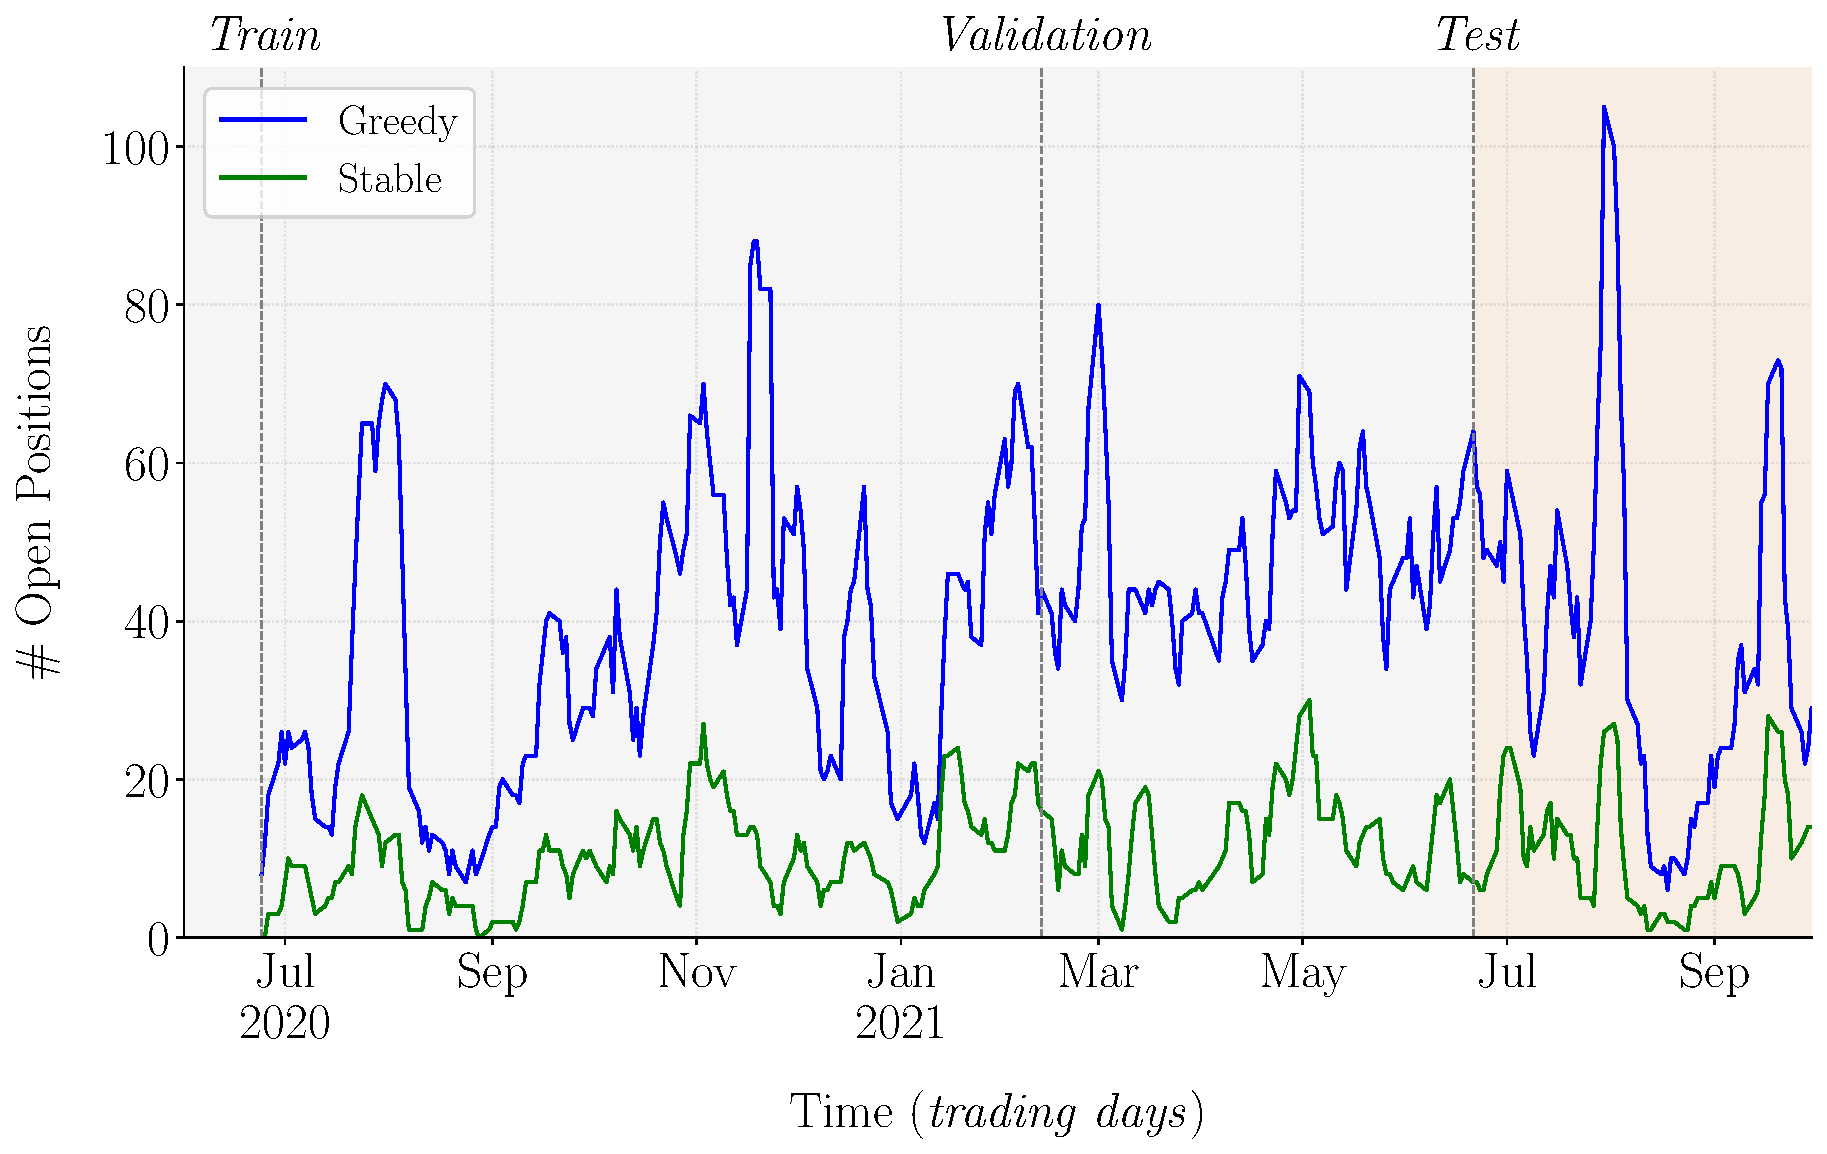
\includegraphics[width=\textwidth]{fig_KMeans_Open_Positions.pdf}
%\end{subfigure}
%\hfill
%\begin{subfigure}[t]{0.49\textwidth}
%\caption{Panel B: LLM Clustering}
%\centering
%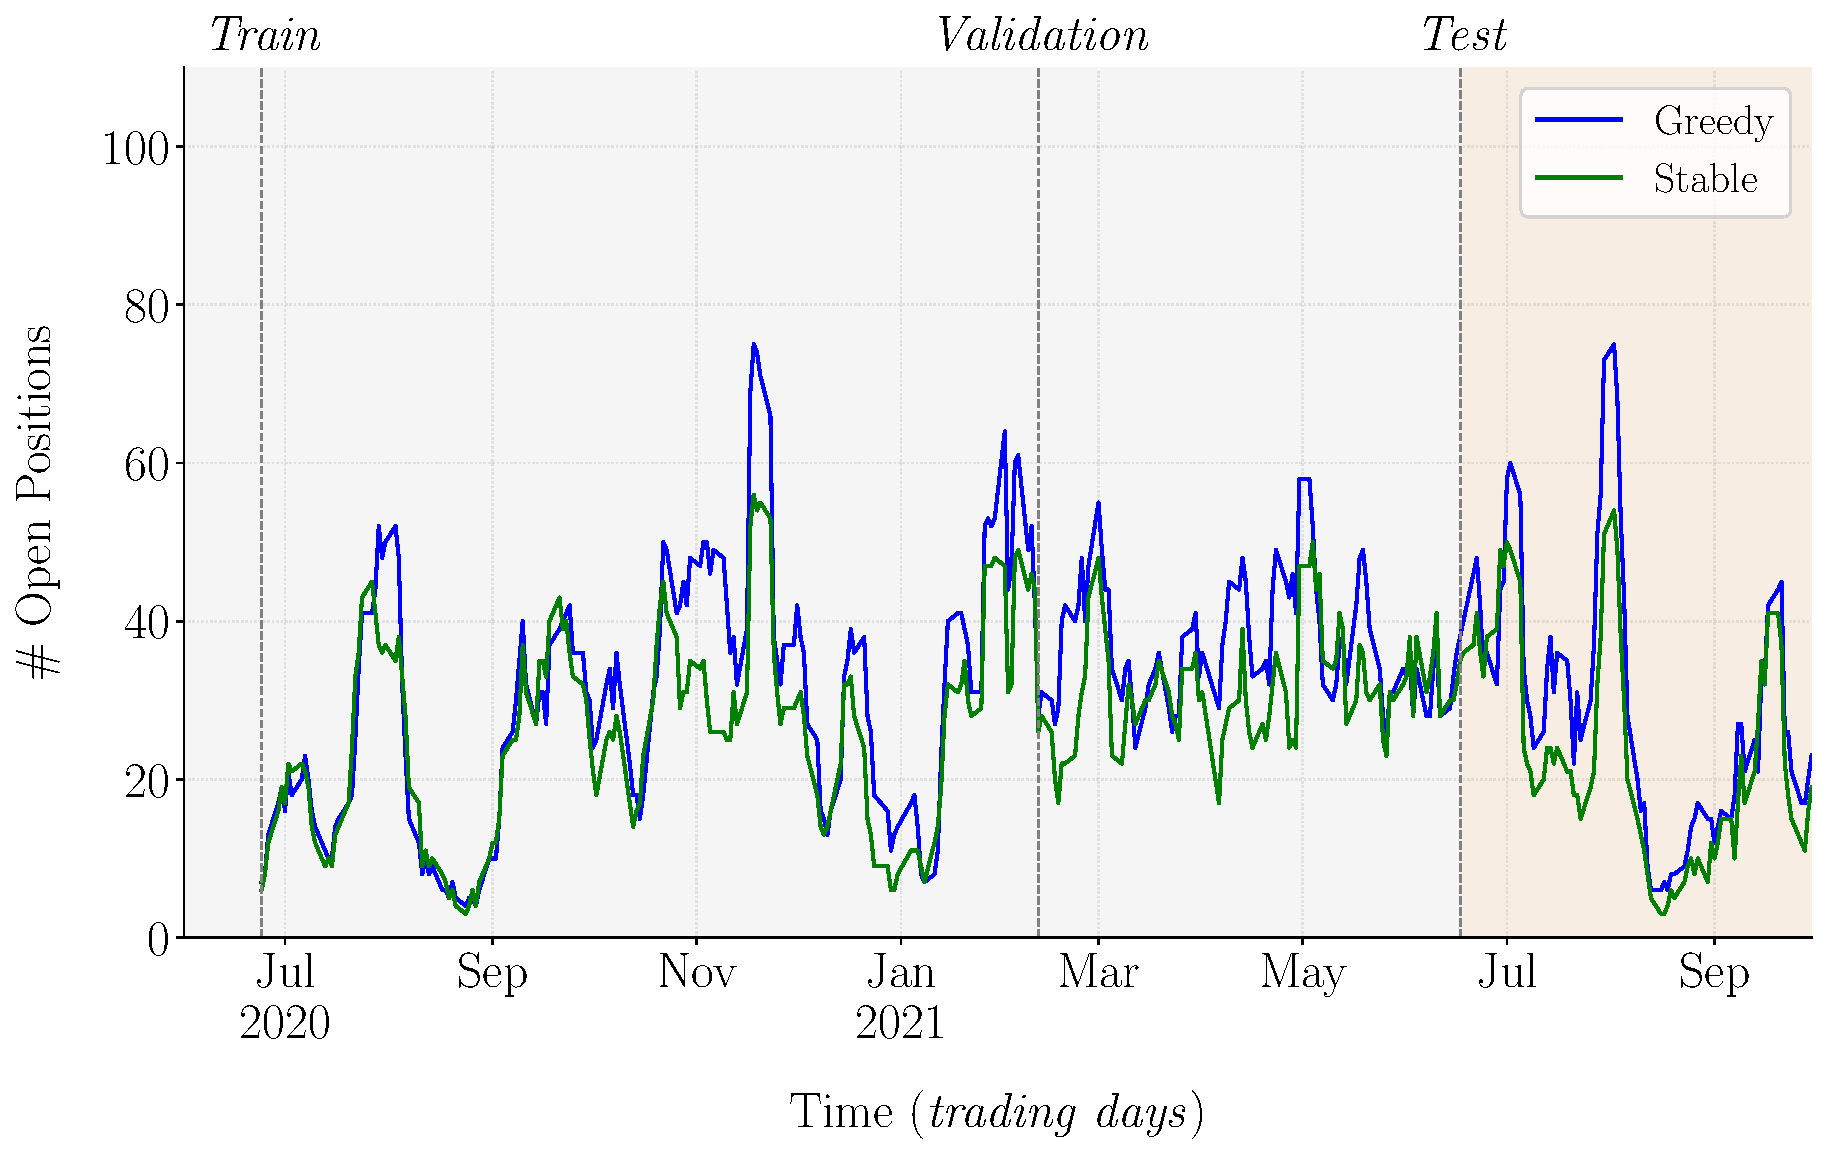
\includegraphics[width=\textwidth]{fig_LLAMA_Open_Positions.pdf}
%\end{subfigure}
%
%\vspace{0.5cm}
%\begin{minipage}{\textwidth}
%\setlength{\parindent}{0pt}
%{\footnotesize\textit{Note:} 
%This figure shows the daily evolution of the number of open positions for both Greedy (blue) and Stable (green) algorithms across different data splits (Train, Validation, Test) using KMeans clustering (Panel A) and LLM clustering (Panel B). The time period spans from July 2020 to September 2021. Vertical dashed lines separate the different data splits. The Greedy algorithm selects clusters that maximize (minimize) the cluster-average-$SR$ for long (short) positions, while the Stable algorithm minimizes the rank difference between training and validation rankings. The number of traded clusters is $\theta = 0.5k=13$ for KMeans ($k^*=26$ clusters) and $\theta = 0.5k=10$ for LLM ($k^*=20$ clusters).
%}
%\end{minipage}
%\end{figure}
%%----------------------------------------------------

%----------------------------------------------------
\inserthere{tab:portfolio_statistics_comparison_net}

\begin{table}[H] 
\caption{Portfolio Statistics Comparison: KMeans vs LLM Clustering (net of Trading Costs)} 
\centering
\label{tab:portfolio_statistics_comparison_net}

\renewcommand{\arraystretch}{1.1}
\newcolumntype{P}[1]{>{\centering\arraybackslash}p{#1}}

% Panel A: KMeans
\begin{subtable}{\textwidth}
\caption{Panel A: Statistics of $\mathcal{P}_{\text{KMeans}}$}
\centering
{\small
\begin{tabular}{
 P{1.28cm} P{0.9cm} P{0.9cm} P{0.9cm} P{0.9cm} P{0.9cm} P{0.9cm} 
 P{0.9cm} P{1cm} P{0.9cm} P{0.9cm} P{0.9cm} P{0.9cm}
}
\Xhline{2\arrayrulewidth}
\textbf{Split} & \textbf{Algo.} & \textbf{Cum. Ret.} & \textbf{Avg. Ret.} & \textbf{St. Dev.} & \textbf{Sharpe Ratio} & \textbf{Sortino Ratio} & \textbf{Max. DD} & \textbf{Calmar Ratio} & \textbf{Skew.} & \textbf{Exc. Kurt.} & \textbf{VaR 95\%} & \textbf{CVaR 95\%} \\
\Xhline{2\arrayrulewidth}
\multirow{2}{*}{All} & \textit{Greedy} & 0.780 & -17.3 & 9.6 & -2.0 & -1.7 & -24.7 & -0.7 & -0.48 & 3.90 & -14.0 & -24.2 \\
 & \textit{Stable} & 1.058 & 4.4 & 17.0 & 0.3 & 0.3 & -14.2 & 0.3 & 0.15 & 5.01 & -24.5 & -38.3 \\
\hline
\multirow{2}{*}{Train} & \textit{Greedy} & 0.823 & -25.6 & 11.6 & -2.5 & -2.0 & -18.2 & -1.4 & -0.51 & 2.71 & -19.4 & -29.9 \\
 & \textit{Stable} & 1.057 & 8.7 & 19.9 & 0.4 & 0.4 & -14.2 & 0.6 & -0.25 & 3.21 & -31.9 & -46.0 \\
\hline
\multirow{2}{*}{Validation} & \textit{Greedy} & 1.000 & -0.0 & 7.5 & -0.0 & -0.0 & -5.8 & -0.0 & -0.50 & 0.95 & -12.1 & -17.9 \\
 & \textit{Stable} & 1.050 & 14.7 & 13.4 & 1.0 & 1.0 & -5.3 & 2.8 & -0.27 & 1.99 & -20.6 & -30.9 \\
\hline
\multirow{2}{*}{Test} & \textit{Greedy} & 0.937 & -20.0 & 6.6 & -3.4 & -3.5 & -9.1 & -2.2 & 1.55 & 4.31 & -8.9 & -12.0 \\
 & \textit{Stable} & 0.924 & -23.6 & 14.2 & -1.9 & -2.0 & -10.0 & -2.4 & 2.48 & 14.59 & -20.6 & -28.5 \\
\Xhline{2\arrayrulewidth}
\end{tabular}
}
\end{subtable}

\vspace{0.5cm}

% Panel B: LLM
\begin{subtable}{\textwidth}
\caption{Panel B: Statistics of $\mathcal{P}_{\text{LLM}}$}
\centering
{\small
\begin{tabular}{
 P{1.28cm} P{0.9cm} P{0.9cm} P{0.9cm} P{0.9cm} P{0.9cm} P{0.9cm} 
 P{0.9cm} P{1cm} P{0.9cm} P{0.9cm} P{0.9cm} P{0.9cm}
}
\Xhline{2\arrayrulewidth}
\textbf{Split} & \textbf{Algo.} & \textbf{Cum. Ret.} & \textbf{Avg. Ret.} & \textbf{St. Dev.} & \textbf{Sharpe Ratio} & \textbf{Sortino Ratio} & \textbf{Max. DD} & \textbf{Calmar Ratio} & \textbf{Skew.} & \textbf{Exc. Kurt.} & \textbf{VaR 95\%} & \textbf{CVaR 95\%} \\
\Xhline{2\arrayrulewidth}
\multirow{2}{*}{All} & \textit{Greedy} & 0.891 & -8.5 & 9.7 & -0.9 & -1.0 & -12.3 & -0.7 & 1.44 & 9.81 & -15.7 & -21.2 \\
 & \textit{Stable} & 0.928 & -5.6 & 8.6 & -0.7 & -0.7 & -11.7 & -0.5 & 0.31 & 2.18 & -12.9 & -18.7 \\
\hline
\multirow{2}{*}{Train} & \textit{Greedy} & 0.910 & -13.4 & 11.5 & -1.2 & -1.3 & -12.3 & -1.1 & 1.63 & 8.83 & -19.4 & -23.2 \\
 & \textit{Stable} & 0.964 & -5.5 & 10.0 & -0.6 & -0.6 & -9.7 & -0.6 & 0.21 & 1.60 & -14.8 & -21.6 \\
\hline
\multirow{2}{*}{Validation} & \textit{Greedy} & 0.985 & -4.3 & 8.1 & -0.5 & -0.6 & -4.3 & -1.0 & 0.19 & 1.17 & -11.6 & -18.0 \\
 & \textit{Stable} & 0.947 & -14.3 & 7.0 & -2.2 & -2.0 & -6.1 & -2.4 & 0.17 & 1.17 & -13.0 & -16.5 \\
\hline
\multirow{2}{*}{Test} & \textit{Greedy} & 0.995 & -1.5 & 6.2 & -0.2 & -0.3 & -1.9 & -0.8 & 1.02 & 6.91 & -8.2 & -12.1 \\
 & \textit{Stable} & 1.009 & 3.1 & 7.0 & 0.4 & 0.5 & -1.8 & 1.7 & 0.91 & 1.98 & -10.8 & -12.4 \\
\Xhline{2\arrayrulewidth}
\end{tabular}
}
\end{subtable}

\vspace{0.5cm}
\begin{minipage}{\textwidth}
\setlength{\parindent}{0pt}
{\small\textit{Note:
Portfolio statistics of trading strategies based on clusters obtained from KMeans (Panel A) and LLM (Panel B) approaches.
The statistics provided include performance metrics (Cumulative Return, Average Return (\%)), risk measures (Standard Deviation (\%), Maximum Drawdown (\%), Value at Risk (\%), Conditional Value at Risk (\%)), risk-adjusted performance ratios (Sharpe Ratio, Sortino Ratio, Calmar Ratio), and return distribution characteristics (Skewness, Excess Kurtosis). These statistics are provided for both cluster-selection algorithms: Greedy and Stable.
Except for the Cumulative Return, all returns are annualized. The Sharpe Ratio is computed using the daily returns, assuming 252 trading days in a year. The Sortino Ratio is calculated using the daily downside returns. The Maximum Drawdown is the maximum loss from a peak to a trough. The Calmar Ratio is the ratio of the annualized return to the maximum drawdown. Skewness measures the asymmetry of the return distribution, while Kurtosis quantifies the tails' thickness. The Value at Risk (VaR) and Conditional Value at Risk (CVaR) are calculated at a 95\% confidence level.
%
All returns are calculated net of transaction costs. We implement a conservative transaction cost estimate of 30 basis points (0.30\%) per trade, which accounts for both direct costs (commissions, fees) and indirect costs (bid-ask spreads, market impact). 
%Transaction costs for each day are computed as the product of daily portfolio turnover and the transaction cost parameter ($TC = \text{turnover} \times 0.30\%$). Daily turnover is measured as the ratio of the absolute change in positions to the total portfolio size: $\text{Turnover} = \sum|Position_{t} - Position_{t-1}| / \sum|Position_{t}|$. This implementation follows standard practice in the literature (see, e.g., \citet{frazzini2012}) and provides a realistic assessment of strategy profitability in real market conditions.
%
The Greedy algorithm longs (shorts) clusters that maximize (minimize) the cluster-average-$SR$ in the validation sample subject to a positivity (negativity) constraint, while the Stable algorithm longs (shorts) clusters that minimize the rank difference between the training and validation rankings of the cluster-average-$SR$'s subject to a positivity (negativity) constraint, which is now imposed on both sample splits. In both algorithms, the cardinality of each leg is upper-bounded by a hyperparameter $\theta$.
The holding period of the beta-neutral positions is set to $L$ = 4 trading days for both approaches. The number of traded clusters is $\theta = 0.5k=13$ for KMeans ($k^*=26$ clusters) and $\theta = 0.5k=10$ for LLM ($k^*=20$ clusters). The selection criteria for these hyperparameters ($L,\theta$) is based on maximizing the Sharpe Ratios of the train and validation samples.
}}
\end{minipage}
\end{table}
%----------------------------------------------------
Finally, the introduction of trading costs significantly impacts the performance metrics of both clustering approaches, though with notably different implications for their practical viability. The KMeans-based strategy exhibits substantial performance degradation, particularly evident in the test period where both algorithms generate significant losses (Greedy: -20.0\%, Stable: -23.6\% average annual returns). This deterioration is accompanied by elevated risk metrics, with the Stable algorithm showing particularly concerning characteristics including high standard deviation (14.2\%) and extreme kurtosis (14.59) in the test period, suggesting frequent occurrence of extreme returns.
In contrast, the LLM-based approach demonstrates superior resilience to trading costs, maintaining more stable performance characteristics across all periods. Most notably, in the test period, the strategy achieves near-neutral to positive performance (Greedy: -1.5\%, Stable: +3.1\% annual returns) with substantially lower risk metrics (standard deviations of 6.2\% and 7.0\% respectively). The LLM approach's more moderate VaR and CVaR measures (around -8.2\% to -12.4\% in the test period) compared to KMeans (-8.9\% to -28.5\%) further underscore its superior risk management characteristics under transaction costs.
This stark contrast in net performance can be attributed to the fundamentally different nature of the signals generated by each approach. While KMeans' statistically-driven clusters require frequent rebalancing that amplifies transaction costs, the LLM's economically-motivated clusters appear to identify more persistent price patterns that remain profitable even after accounting for trading frictions. However, it is worth noting that neither approach was explicitly optimized for transaction cost efficiency, suggesting potential for further improvement through cost-aware portfolio construction. These results highlight that while our LLM-based news parser successfully captures predictable market reactions to news articles, practitioners implementing such strategies would benefit from incorporating transaction costs into their optimization framework.

%As we can see, given that the trading intensity is really high, the profitability of the trading strategy out of sample is reduced substantially. The trading strategy has not been optimized to account for trading costs and is therefore sensitive to them. The objective of the trading strategy was to identify winners and losers by reading news articles with the sole purpose of anticipating market trends. The exercise we did was about discovering the predictability of market reactions to news articles by designing an LLM-based news parser. A trader interested in this application would prefer to optimize the trading strategy to make it robust to trading costs. 

%%%%%%%%%%%%%%%%% CONCLUSION %%%%%%%%%%%%%%%%%%%%%%
%----------------------------------------------------
\section{Conclusion}
%----------------------------------------------------
%\hspace{0.5cm} 
This paper investigates how information from business news affects stock market prices. We analyze a dataset of Spanish business articles during a particularly volatile period-the COVID-19 pandemic-and examine firm-specific stock market reactions to news. We show that transforming text into vector embeddings and clustering them using KMeans yields clusters that are firm-specific and industry-specific. However, the distribution of articles across clusters is unstable over sequential data splits, indicating temporal instability. When we implement a cluster-based trading strategy-similar to portfolio sorts-on the KMeans clusters, we observe an over-reliance on the past performance of a cluster. That is, signals are short-lived due to temporal instability. Consequently, the out-of-sample profitability of the trading strategy is negligible, evidencing the method's poor temporal generalizability. Therefore, a model based on embeddings is superficial and is not able to anticipate market trends.

%----------------------------------------------------
Alternatively, we develop a novel approach by guiding a Large Language Model (LLM) through a structured news-parsing schema, enabling it to analyze news-implied firm-specific economic shocks. The schema involves identifying the firms affected by the articles and classifying the implied shocks on such firms by their type, magnitude, and direction. This LLM-based methodology demonstrates several advantages over the traditional clustering approach. Even in a volatile period, it produces stable distributions of articles across clusters in sequential splits, demonstrating robust temporal stability. Moreover, the resulting trading signals are both long-lasting and economically relevant, as they are based on fundamental economic shocks rather than statistical patterns. The results show that the LLM-based trading strategy effectively identifies winners and losers, illustrating the parser's ability to anticipate market trends by comprehending the economic implications of firm-specific shocks. This approach generates a consistent profile of earnings in the test set, with results robust to the choice of hyperparameters-the holding period length of the trading strategy and the number of selected clusters for trading. Our findings demonstrate a promising avenue: LLMs, when guided by appropriate economic frameworks, can help predict market reactions to news through systematic classification of economic shocks embedded in financial narratives.


%%%%%%%%%%%%%%%%%% BIBLIOGRAPHY %%%%%%%%%%%%%%%%%%%%%%
\bibliography{bib_references_DOI.bib}
%\bibliographystyle{plain}
\bibliographystyle{elsarticle-num}
%----------------------------------------------------
\newpage
% To make sure all the tables/figures appear before the appendix
\processdelayedfloats 
% Reset the numbering for appendix figures and tables
\renewcommand{\thefigure}{A\arabic{figure}} 
\renewcommand{\thetable}{A\arabic{table}}
%----------------------------------------------------

%%%%%%%%%%%%%%%%%% APPENDIX %%%%%%%%%%%%%%%%%%%%%%
\appendix
\section{Appendix}
% 1) KMeans Algorithm
%%%%%%%%%%%%%%%%%%%%%%%%%%%%%%%%%%%%%%%%%%%%%%%%%%%%%
\subsection{KMeans Algorithm}
\begin{algorithm}[H]
\caption{KMeans Clustering Algorithm}
\label{alg:KMeans}
\begin{algorithmic}[1]
\State \textbf{Input:} Embedding vectors $\{\mathbf{e}^1, \mathbf{e}^2, \ldots, \mathbf{e}^{N}\}$, number of clusters $k$
\State \textbf{Output:} Cluster assignments $\{\D_1, \D_2, \ldots, \D_k\}$, centroids $\{\mathbf{c}_1, \mathbf{c}_2, \ldots, \mathbf{c}_k\}$

\State \textbf{Initialize} centroids $\{\mathbf{c}_1, \mathbf{c}_2, \ldots, \mathbf{c}_k\}$ randomly

\Repeat
    \State \underline{\textit{Assignment Step:}}
    \For{each vector $\mathbf{e}^i$}
        \State Assign $\mathbf{e}^i$ to the nearest centroid:
        \[
        g = \arg \min_{\ell\in\{1,...,k\}} \|\mathbf{e}^i - \mathbf{c}_{\ell}\|_{2}^2
        \]
        \State Update cluster assignments: $\D_{g} \leftarrow \D_{g} \cup \{i\}$
    \EndFor

    \State \underline{\textit{Update Step:}}
    \For{each cluster $\D_g$}
        \State Recalculate centroid $\mathbf{c}_g$:
        \[
        \mathbf{c}_g = \frac{1}{|\D_g|} \sum_{i \in \D_g} \mathbf{e}^i
        \]
    \EndFor
\Until{cluster assignments no longer change}

\State \textbf{Return} cluster assignments $\{\D_1, \D_2, \ldots, \D_k\}$ and centroids $\{\mathbf{c}_1, \mathbf{c}_2, \ldots, \mathbf{c}_k\}$

\end{algorithmic}
\end{algorithm}

%%%%%%%%%%%%%%%%%%%%%%%%%%%%%%%%%%%%%%%%%%%%%%%%%%%%%

\newpage
% 2) Hyperparameter Justification
%%%%%%%%%%%%%%%%%%%%%%%%%%%%%%%%%%%%%%%%%%%%%%%%%%%%%
\subsection{Hyperparameter Choice}
Our hyperparameters are $L$ and $\theta$. Recall that $L$ denotes the number of trading days over which we hold the positions in the beta-neutral strategy, while $\theta$ represents the upper bound on each side (long and short) for the amount of clusters we select for the trading strategy. The specific choice of hyperparameters we made for the results presented in the paper were:
\begin{align*}
L &= 4
\\
\theta &= \integer{0.5k}
\end{align*}
where $k$ represents the number of clusters (26 for KMeans clustering, and 20 for LLM clustering). This choice is not arbitrary nor opportunistic. Instead, it results from the maximization of the Sharpe Ratio of the portfolio in the train and validation samples for both KMeans and LLM clustering. This choice procedure is completely based on \textit{in-sample} criteria and it prevents lookahead bias. The justification for such choices is made below.

\subsubsection{KMeans Clustering}

In \cref{fig:KMeans_hyperparameter_justification_L} we can see that a choice of $L=4$ in the training and validation splits generates the most stable Sharpe Ratio. Namely, In the train set (\cref{fig:K_hyp_1}), it makes more sense to choose low values of $L$ (less than 4) to maximize the $SR$. However, in the validation set (\cref{fig:K_hyp_2}), it makes more sense to choose higher values of $L$. The choice of $L=4$ represents a balanced compromise, providing a stable Sharpe Ratio profile across both splits, ensuring consistent in-sample performance.
%The choice of $L=4$ stands as a middle ground between this contradiction, generating a stable choice and a stable profile of earnings in sample.

\setcounter{figure}{0}
%----------------------------------------------------
\inserthere{fig:KMeans_hyperparameter_justification_L}
\begin{figure}[H]
  \caption{Sharpe Ratios in the train and validation splits as a function of $L$ (KMeans)}
  \centering
  
  \begin{subfigure}[b]{0.46\textwidth}
    \centering
    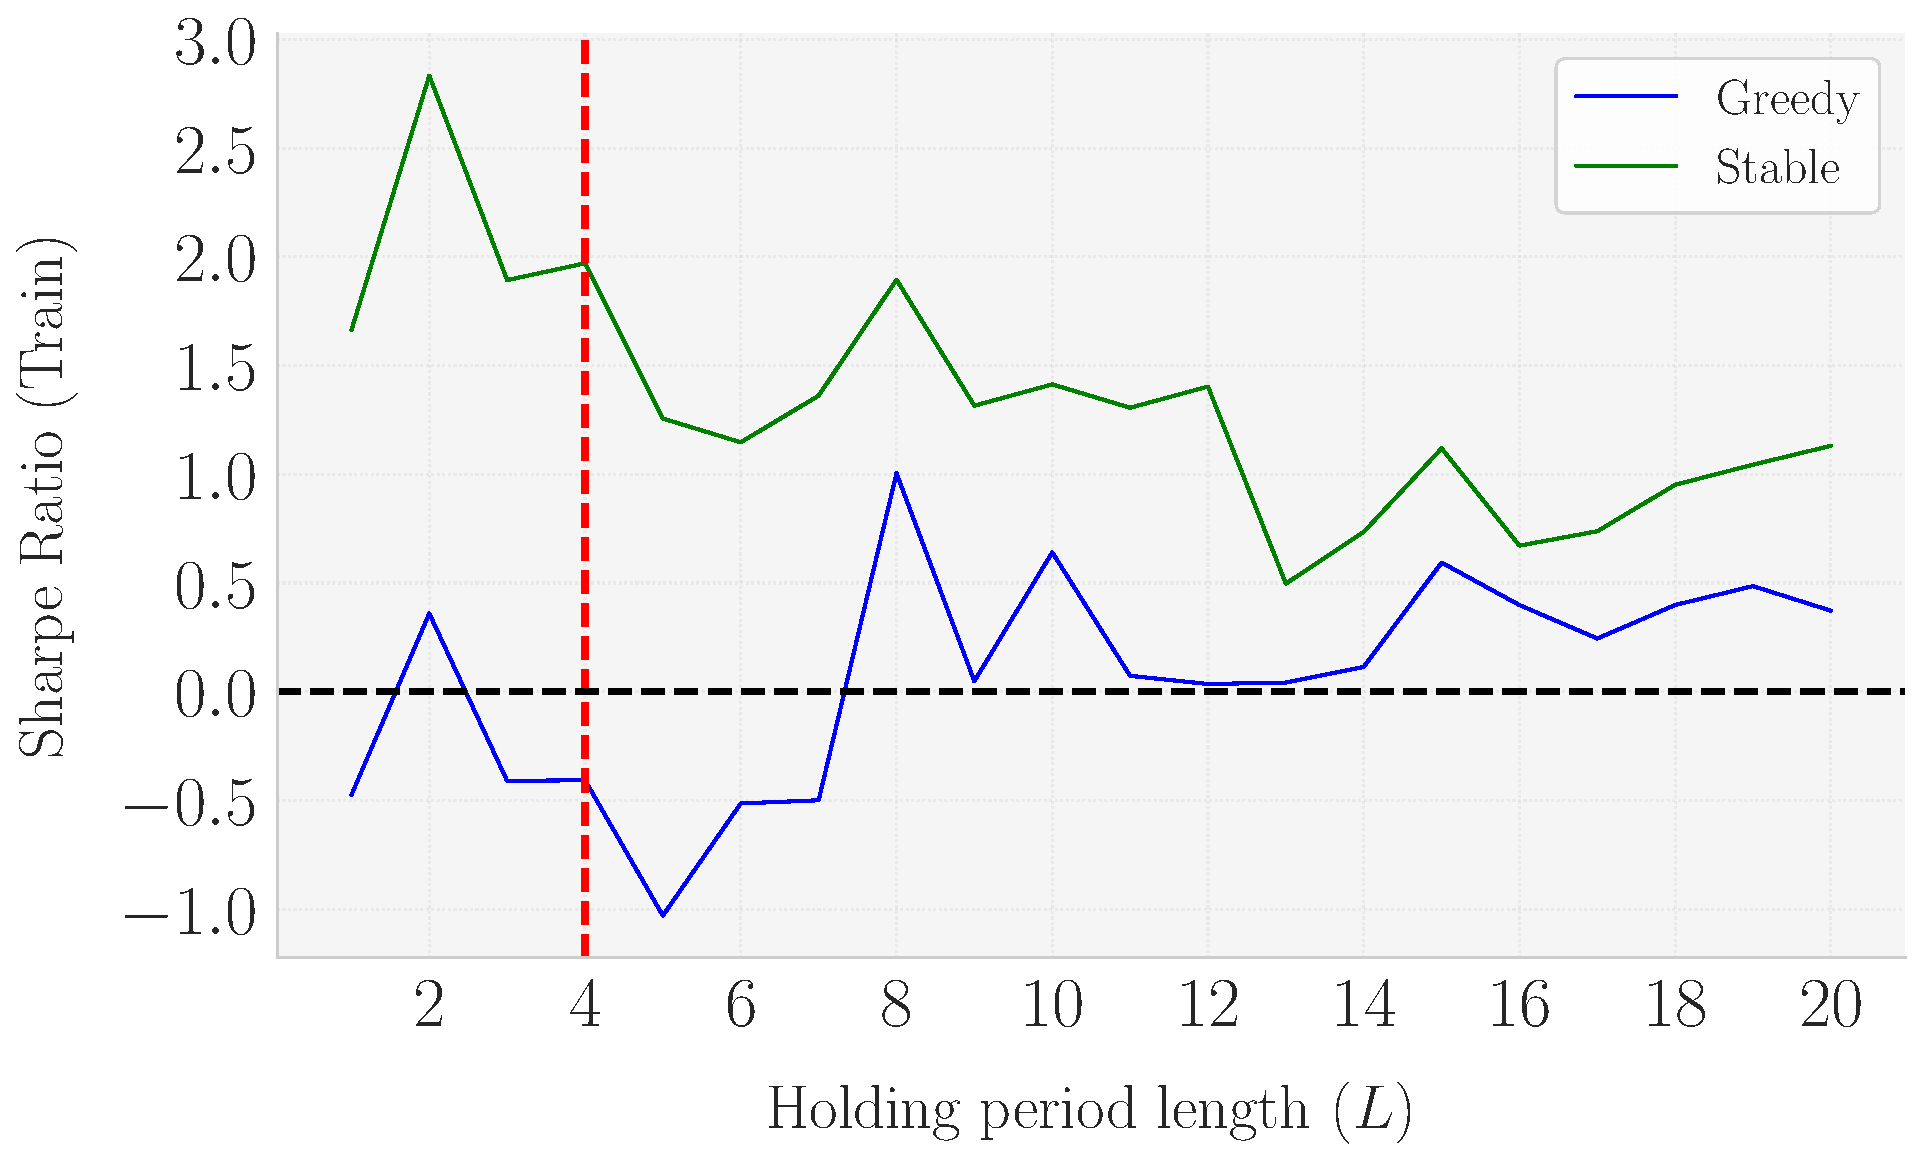
\includegraphics[width=\textwidth]{fig_A1a_KMeans_SR_Train_vs_L.pdf}
    \caption{Plot of $SR^{\mathcal P^{tr}}(L)$ over a grid of $L$}
    \label{fig:K_hyp_1}
  \end{subfigure}
  \hspace{0.05\textwidth} % Add horizontal space between the subfigures
  \begin{subfigure}[b]{0.46\textwidth}
    \centering
    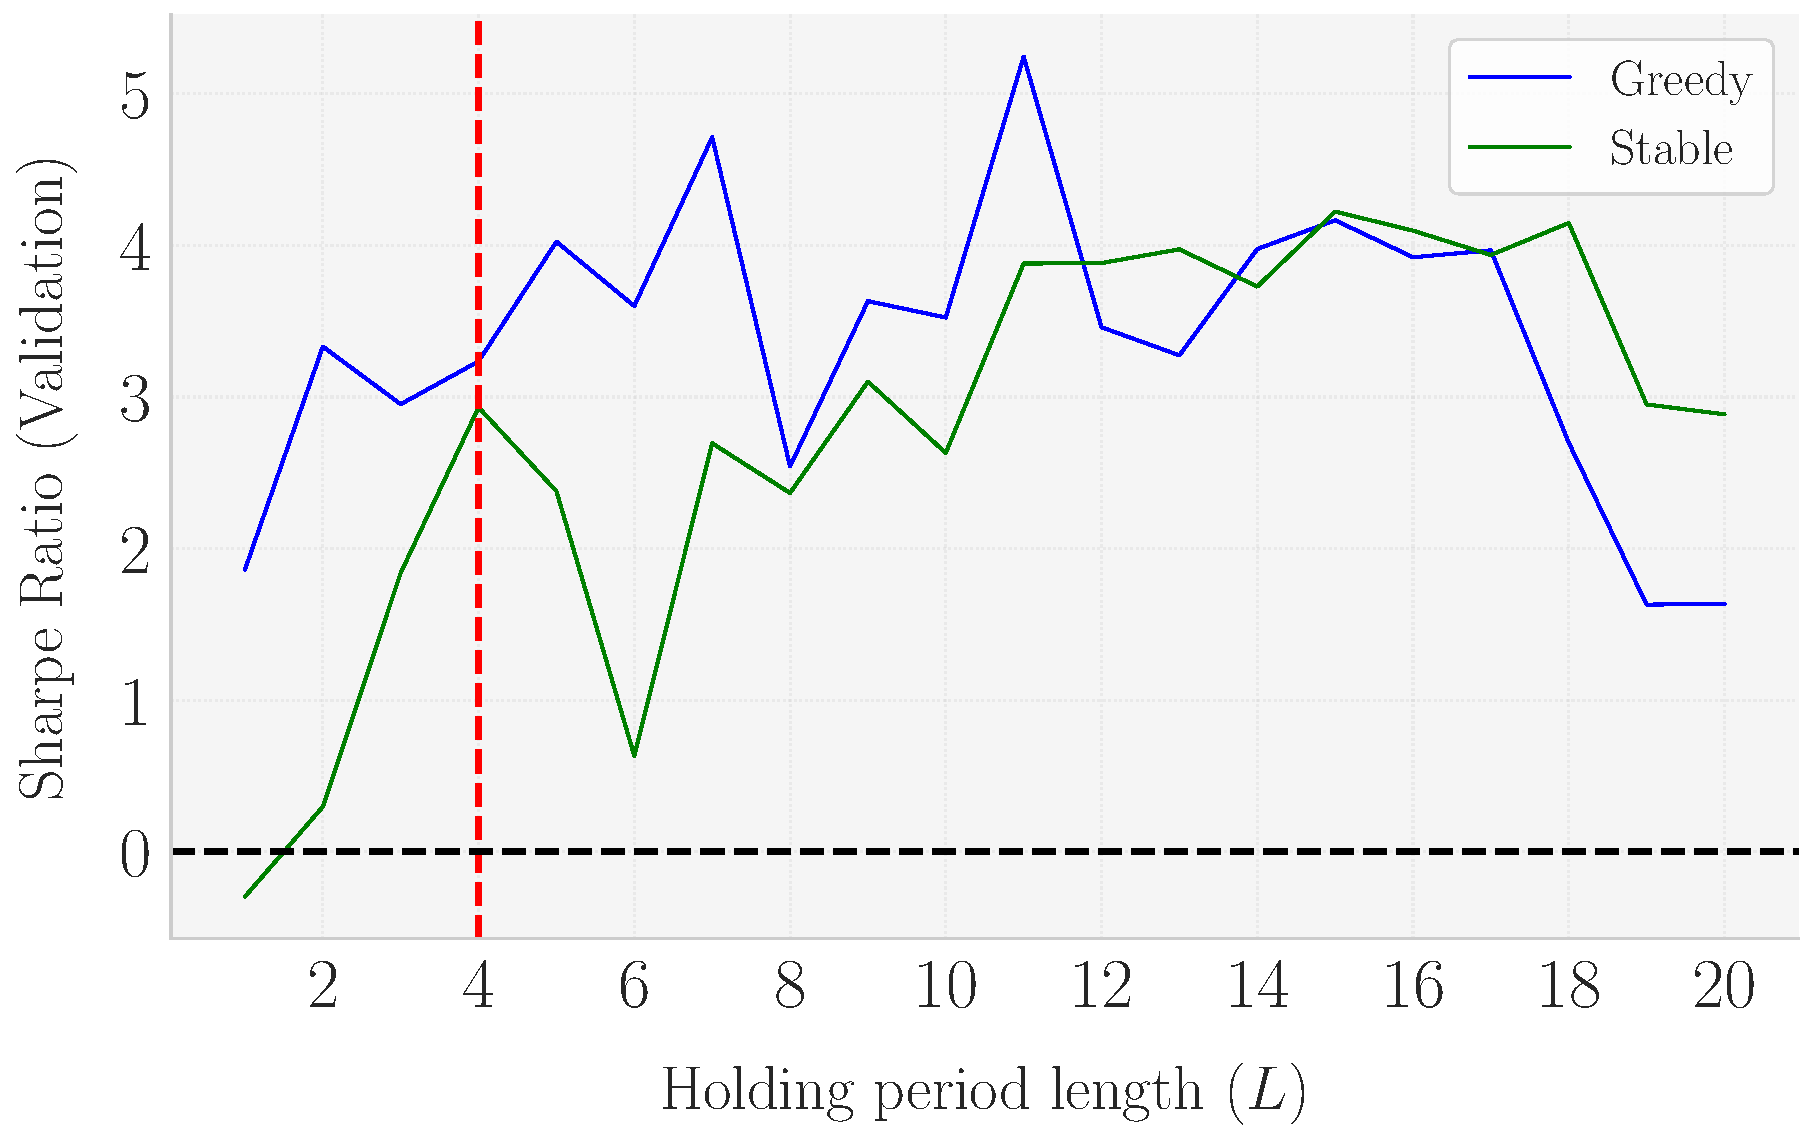
\includegraphics[width=\textwidth]{fig_A1b_KMeans_SR_Validation_vs_L.pdf}
    \caption{Plot of $SR^{\mathcal P^{val}}(L)$ over a grid of $L$}
    \label{fig:K_hyp_2}
  \end{subfigure}  
  \mx
  \subcaption*{\textit{Note: This figure shows the Sharpe Ratios ($SR$) as a function of the holding period length ($L$) for the KMeans clustering method in the training (Panel a) and validation (Panel b) splits. In Panel (a), the Sharpe Ratios in the training set indicate that lower values of $L$ (less than 4) maximize performance. Conversely, in Panel (b), the validation set shows higher Sharpe Ratios for longer holding periods. The choice of $L=4$ represents a balanced compromise, providing a stable Sharpe Ratio profile across both splits, ensuring consistent in-sample performance without introducing lookahead bias.}}
  \label{fig:KMeans_hyperparameter_justification_L}
\end{figure}
%----------------------------------------------------

On the other hand, the choice of $\theta=\integer{0.5\cd 26}=13$ is a choice that pursues stability in the Sharpe Ratio of the train and validation portfolios. As we can see from \cref{fig:KMeans_hyperparameter_justification_theta}, the Sharpe Ratios tend to converge to the highest and most stable value when we choose the highest possible value of $\theta$. 

 %----------------------------------------------------
\inserthere{fig:KMeans_hyperparameter_justification_theta}
\begin{figure}[H]
  \caption{Sharpe Ratios in the train and validation splits as a function of $\theta$ (KMeans)}
  \centering
    \begin{subfigure}[b]{0.46\textwidth}
    \centering
    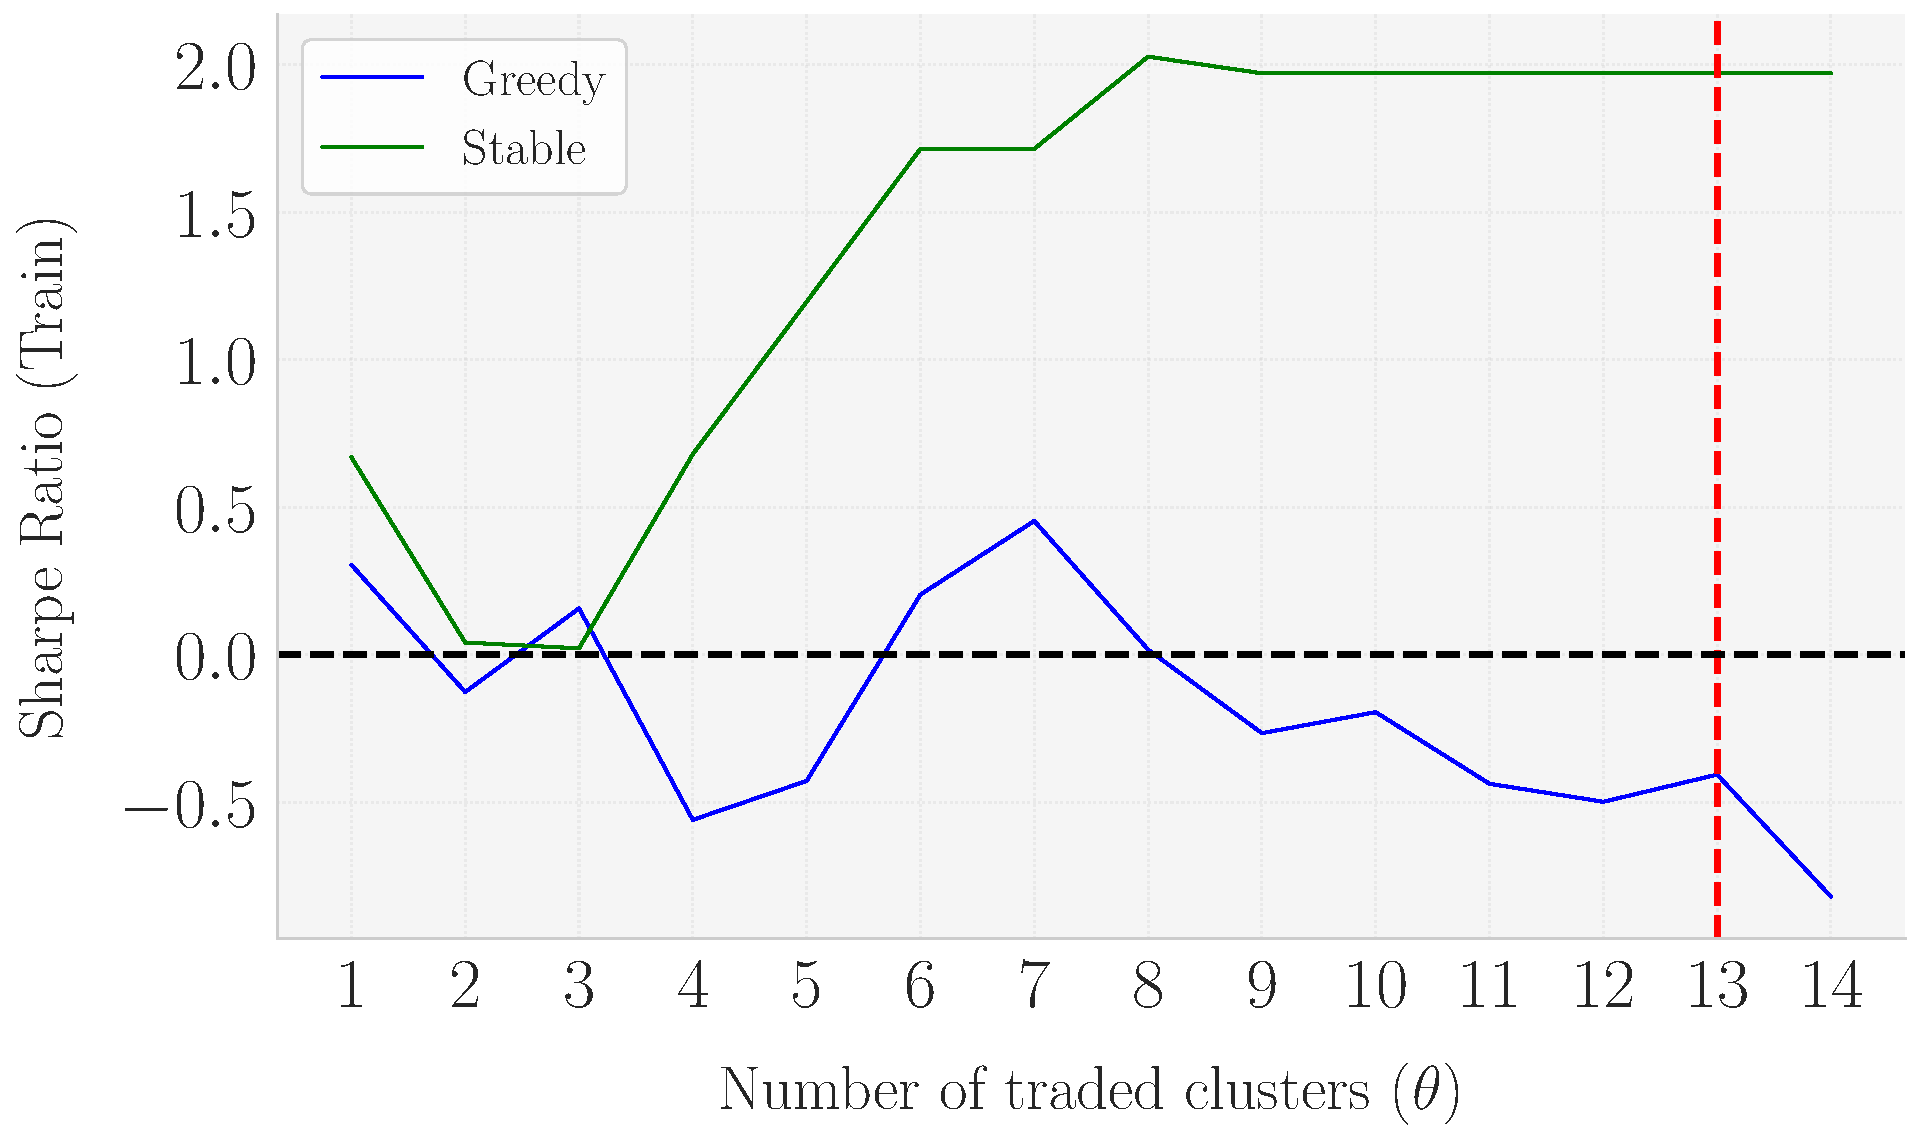
\includegraphics[width=\textwidth]{fig_A2a_KMeans_SR_Train_vs_theta.pdf}
    \caption{Plot of $SR^{\mathcal P^{tr}}(\theta)$ over a grid of $\theta$}
    \label{fig:K_hyp_3}
  \end{subfigure}
  \hspace{0.05\textwidth} % Add horizontal space between the subfigures
  \begin{subfigure}[b]{0.46\textwidth}
    \centering
    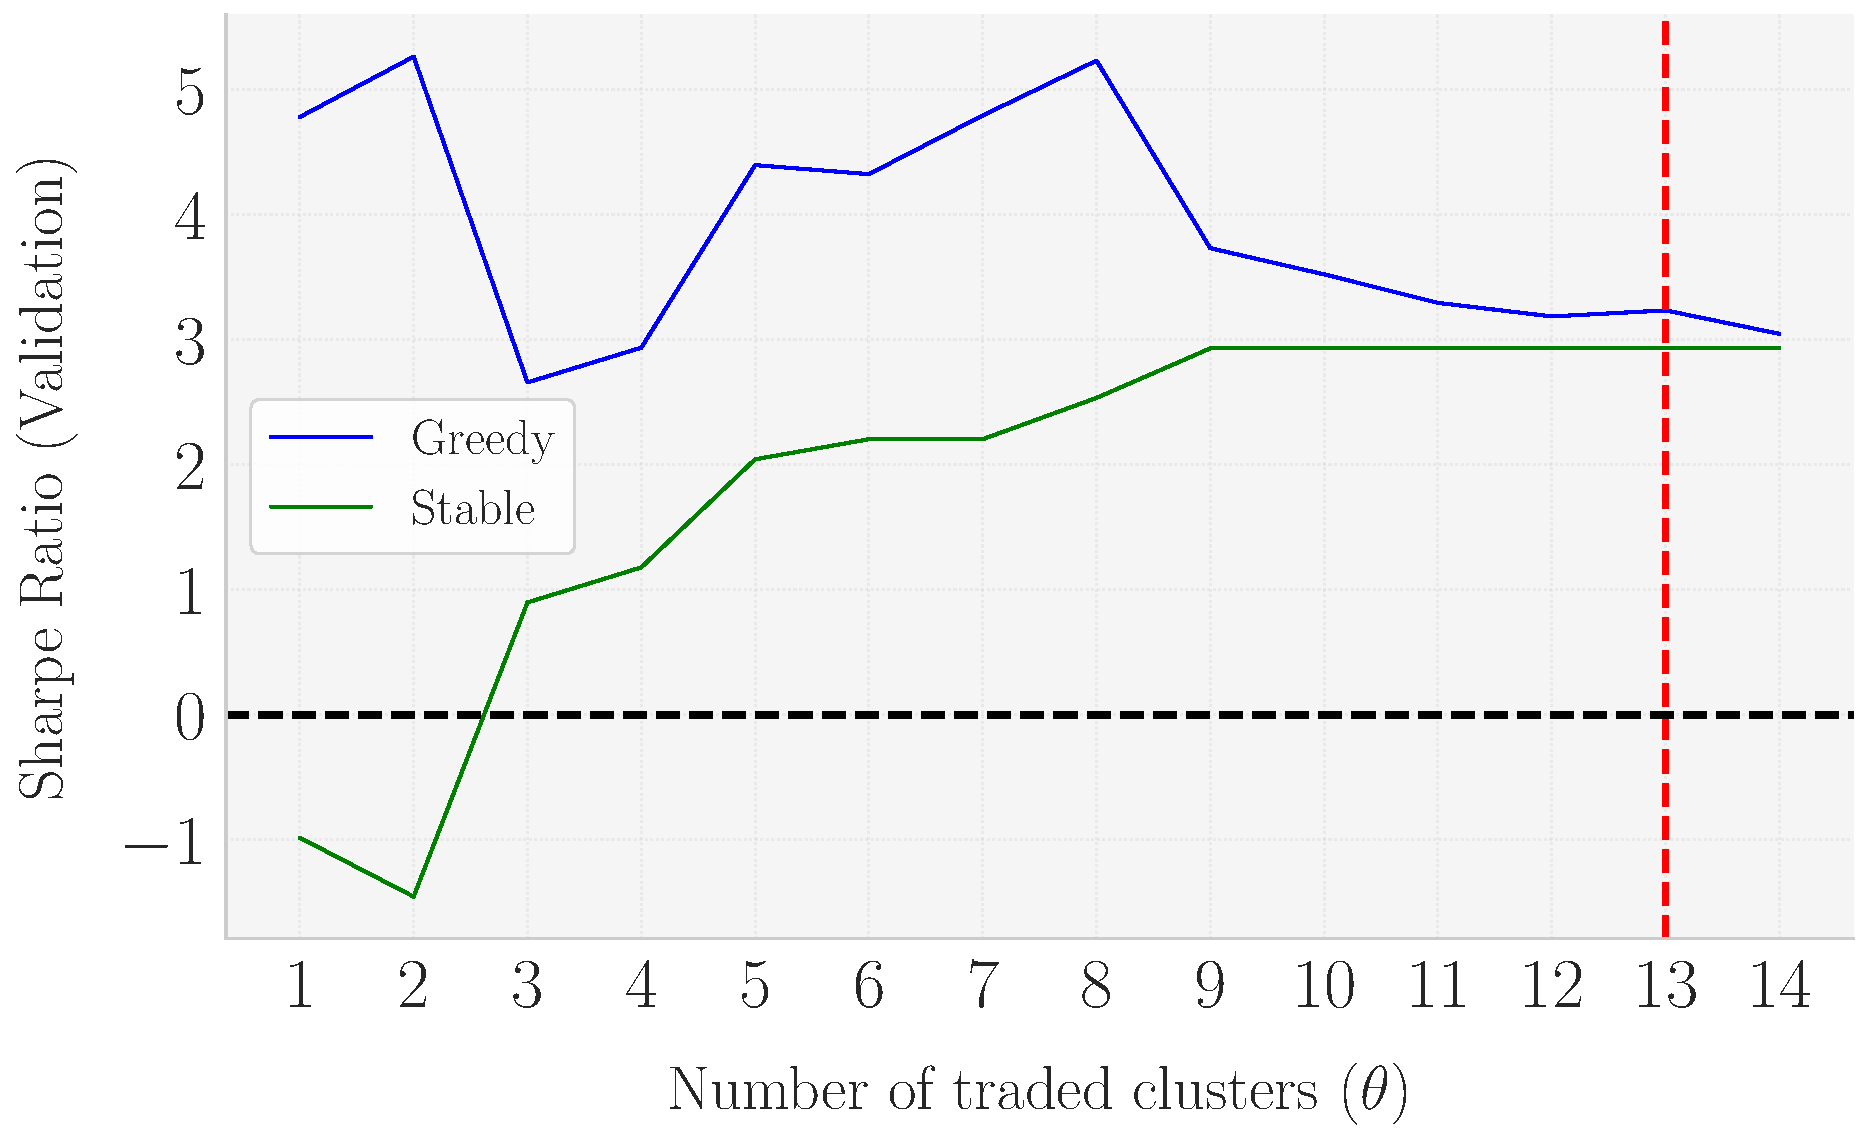
\includegraphics[width=\textwidth]{fig_A2b_KMeans_SR_Validation_vs_theta.pdf}
    \caption{Plot of $SR^{\mathcal P^{val}}(\theta)$ over a grid of $\theta$}
    \label{fig:K_hyp_4}
  \end{subfigure}
  \mx
\subcaption*{\textit{Note: This figure illustrates the Sharpe Ratios ($SR$) as a function of $\theta$, the upper bound on the number of traded clusters, for the KMeans clustering method in the training (Panel a) and validation (Panel b) splits. In Panel (a), the Sharpe Ratios in the training set show a trend of increasing stability and maximizing performance as $\theta$ approaches its upper limit. Similarly, Panel (b) displays a consistent pattern in the validation set, where higher values of $\theta$ lead to convergence at the highest and most stable Sharpe Ratios. The choice of $\theta = 13$ (i.e: $\integer{0.5 \cdot 26}$) reflects this observed stability and optimization, providing a balanced and robust selection for the portfolio strategy.}}
  \label{fig:KMeans_hyperparameter_justification_theta}
\end{figure}
%----------------------------------------------------


\subsubsection{LLM Clustering}
Following a similar logic as below, the choice of $L=4$ sets a consensus between the maximization of $SR^{\mathcal P^{tr}}$ and $SR^{\mathcal P^{val}}$. That is, maximizing $SR^{\mathcal P^{tr}}$ requires lower holding period lengths (the maximizer is $L=4$), while maximizing $SR^{\mathcal P^{val}}$ requires increasing the window length. Among this contradiction, from \cref{fig:LLM_hyperparameter_justification_L} it follows that $L=4$ stands as a perfect choice to balance the maximization requirements in both samples, generating a stable choice for the holding period window length.

%----------------------------------------------------
\inserthere{fig:LLM_hyperparameter_justification_L}
\begin{figure}[H]
  \caption{Sharpe Ratios in the train and validation splits as a function of hyperparameters (LLM)}
  \centering
  
  \begin{subfigure}[b]{0.46\textwidth}
    \centering
    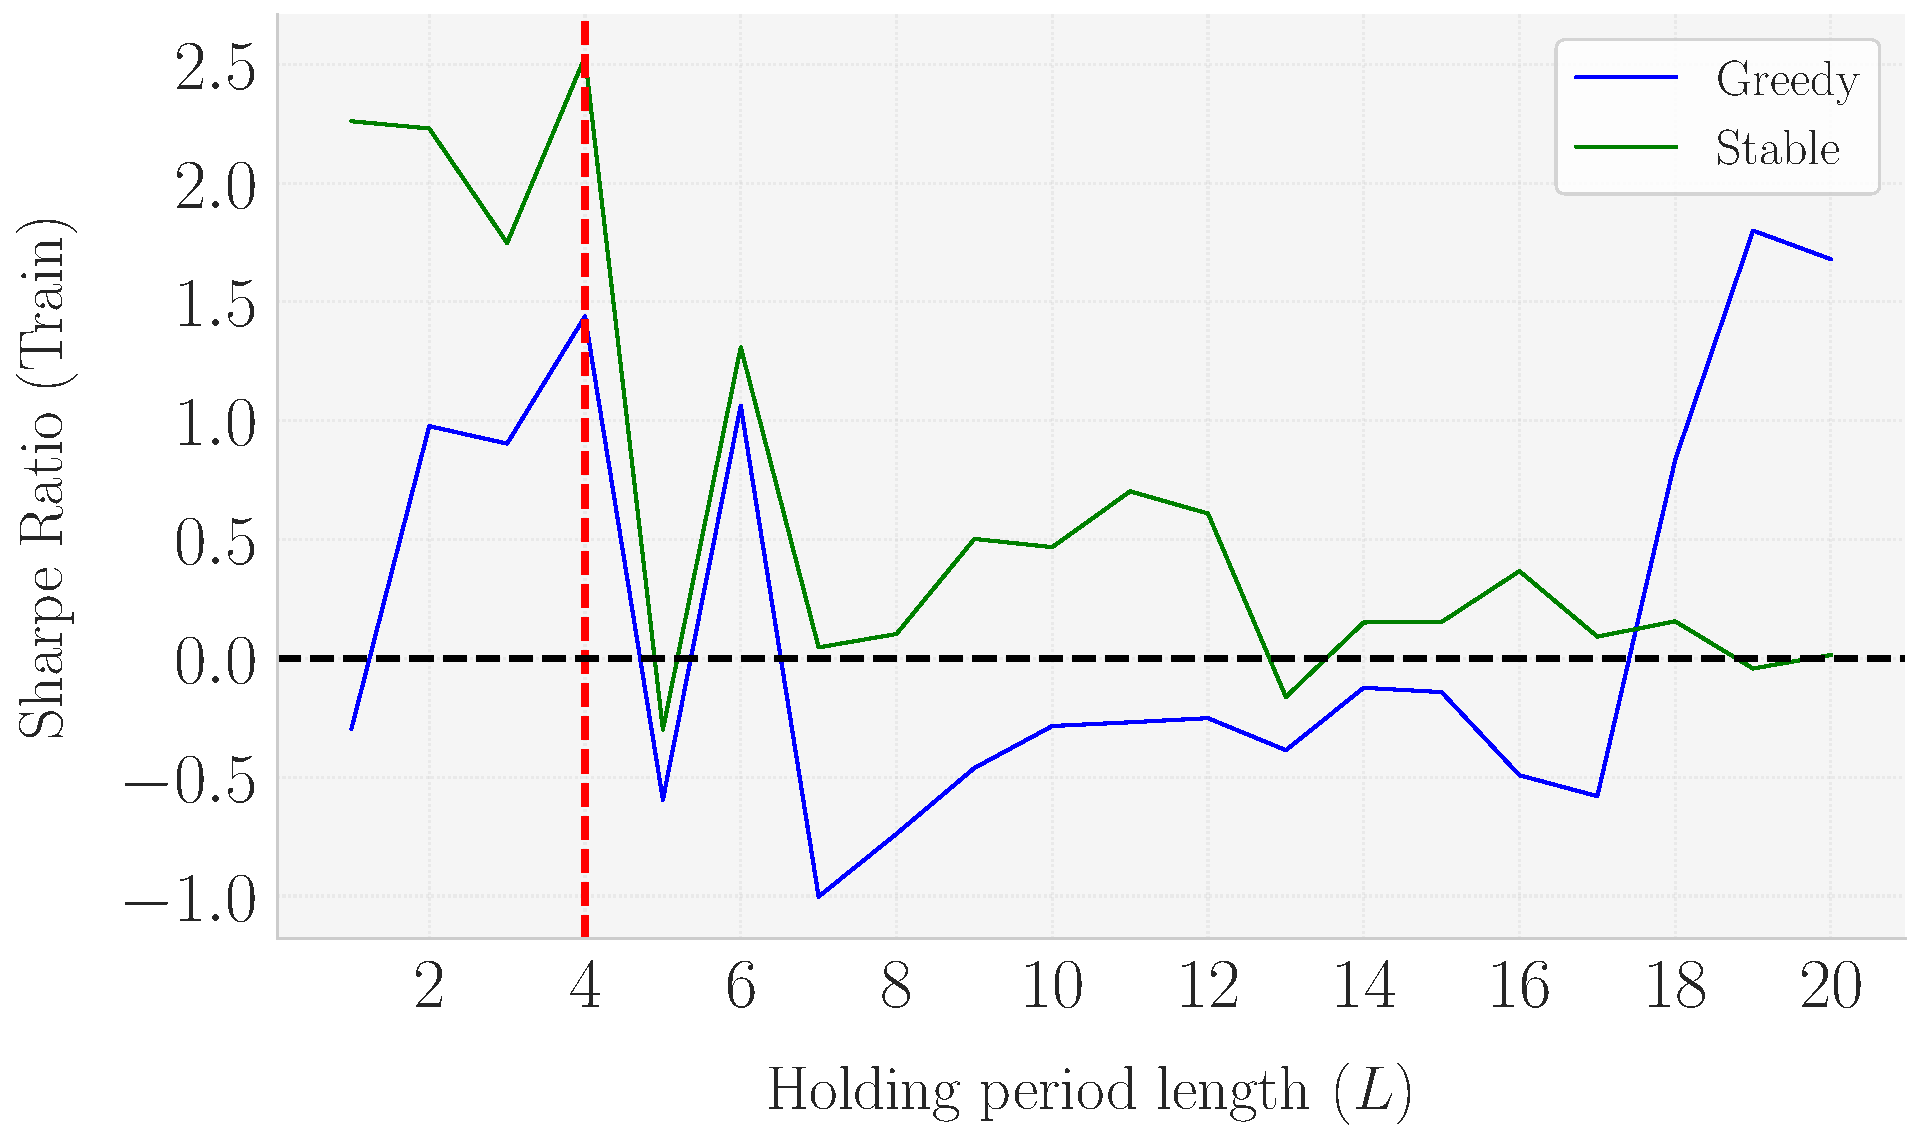
\includegraphics[width=\textwidth]{fig_A3a_LLAMA_SR_Train_vs_L.pdf}
    \caption{Plot of $SR^{\mathcal P^{tr}}(L)$ over a grid of $L$}
    \label{fig:LLM_hyp_1}
    
  \end{subfigure}
  \hspace{0.05\textwidth} % Add horizontal space between the subfigures
  \begin{subfigure}[b]{0.46\textwidth}
    \centering
    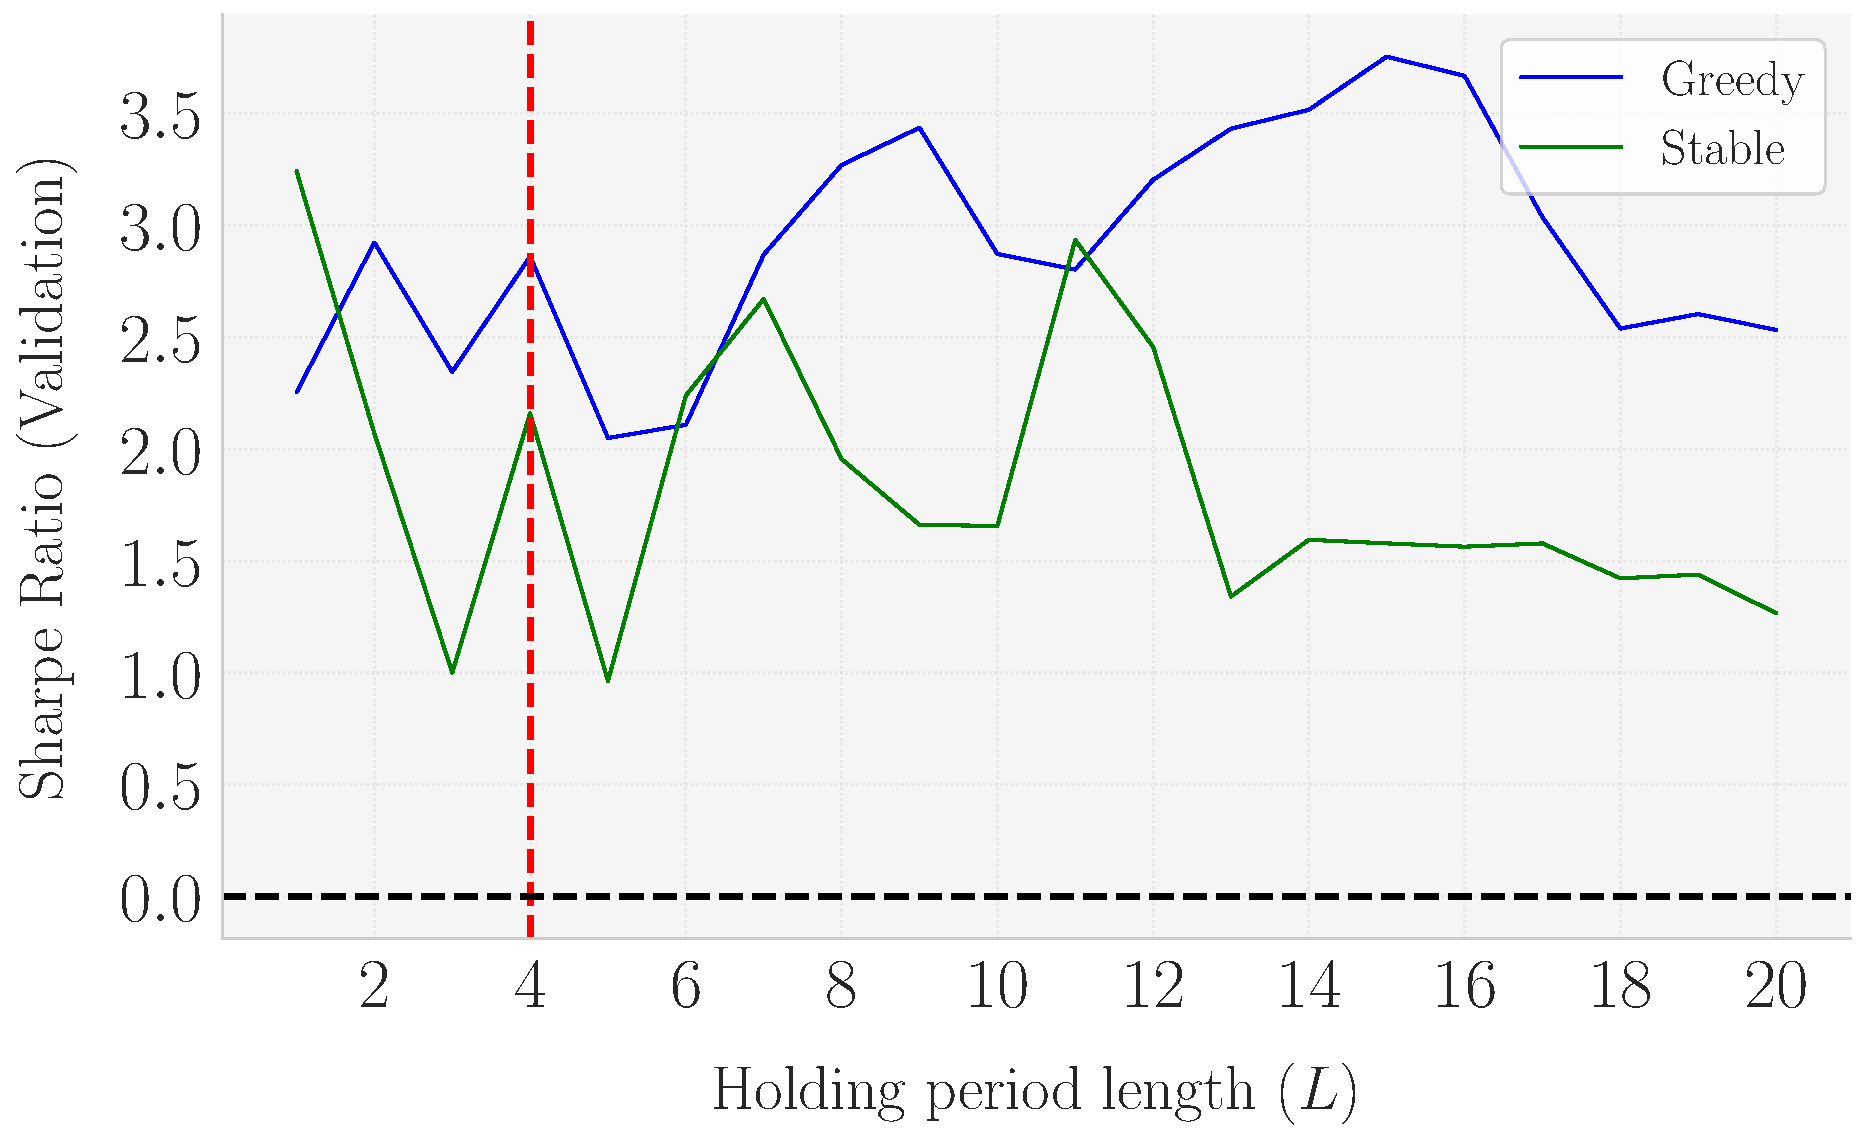
\includegraphics[width=\textwidth]{fig_A3b_LLAMA_SR_Validation_vs_L.pdf}
    \caption{Plot of $SR^{\mathcal P^{val}}(L)$ over a grid of $L$}
    \label{fig:LLM_hyp_2}
  \end{subfigure}
  \mx 
  \subcaption*{\textit{Note: This figure shows the Sharpe Ratios ($SR$) as a function of the holding period length ($L$) for the LLM clustering method, across the training (Panel a) and validation (Panel b) splits. In Panel (a), the Sharpe Ratios in the training set reach their maximum at $L=4$, suggesting shorter holding periods are more effective for maximizing performance. Conversely, Panel (b) illustrates that longer holding periods yield higher Sharpe Ratios in the validation set. The choice of $L=4$ serves as a compromise, balancing the trade-off between maximizing $SR$ in both splits and providing a stable and consistent holding period length for the strategy.}}
  \label{fig:LLM_hyperparameter_justification_L}
\end{figure}
%----------------------------------------------------

Finally, the same conclusion as in KMeans applies here. By selecting $\theta=\integer{0.5\cd 20}=10$, we get a stable Sharpe Ratio. Even though we observe that $SR^{\mathcal P^{tr}}(L)$ falls momentarily at $\theta=10$ for the Greedy algorithm, it still constitutes a good choice. Conversely, at $\theta=10$ the greedy algorithm sees a jump in $SR^{\mathcal P^{val}}(L)$ (see \cref{fig:LLM_hyperparameter_justification_theta}). All in all, we can easily conclude that $\theta=\integer{0.5k}$ arises as a good hyperpamrameter choice also for LLM clustering.
%----------------------------------------------------
\inserthere{fig:LLM_hyperparameter_justification_theta}
\begin{figure}[H]
\caption{Sharpe Ratios in the train and validation splits as a function of $\theta$ (LLM)}
  \centering

    \begin{subfigure}[b]{0.46\textwidth}
    \centering
    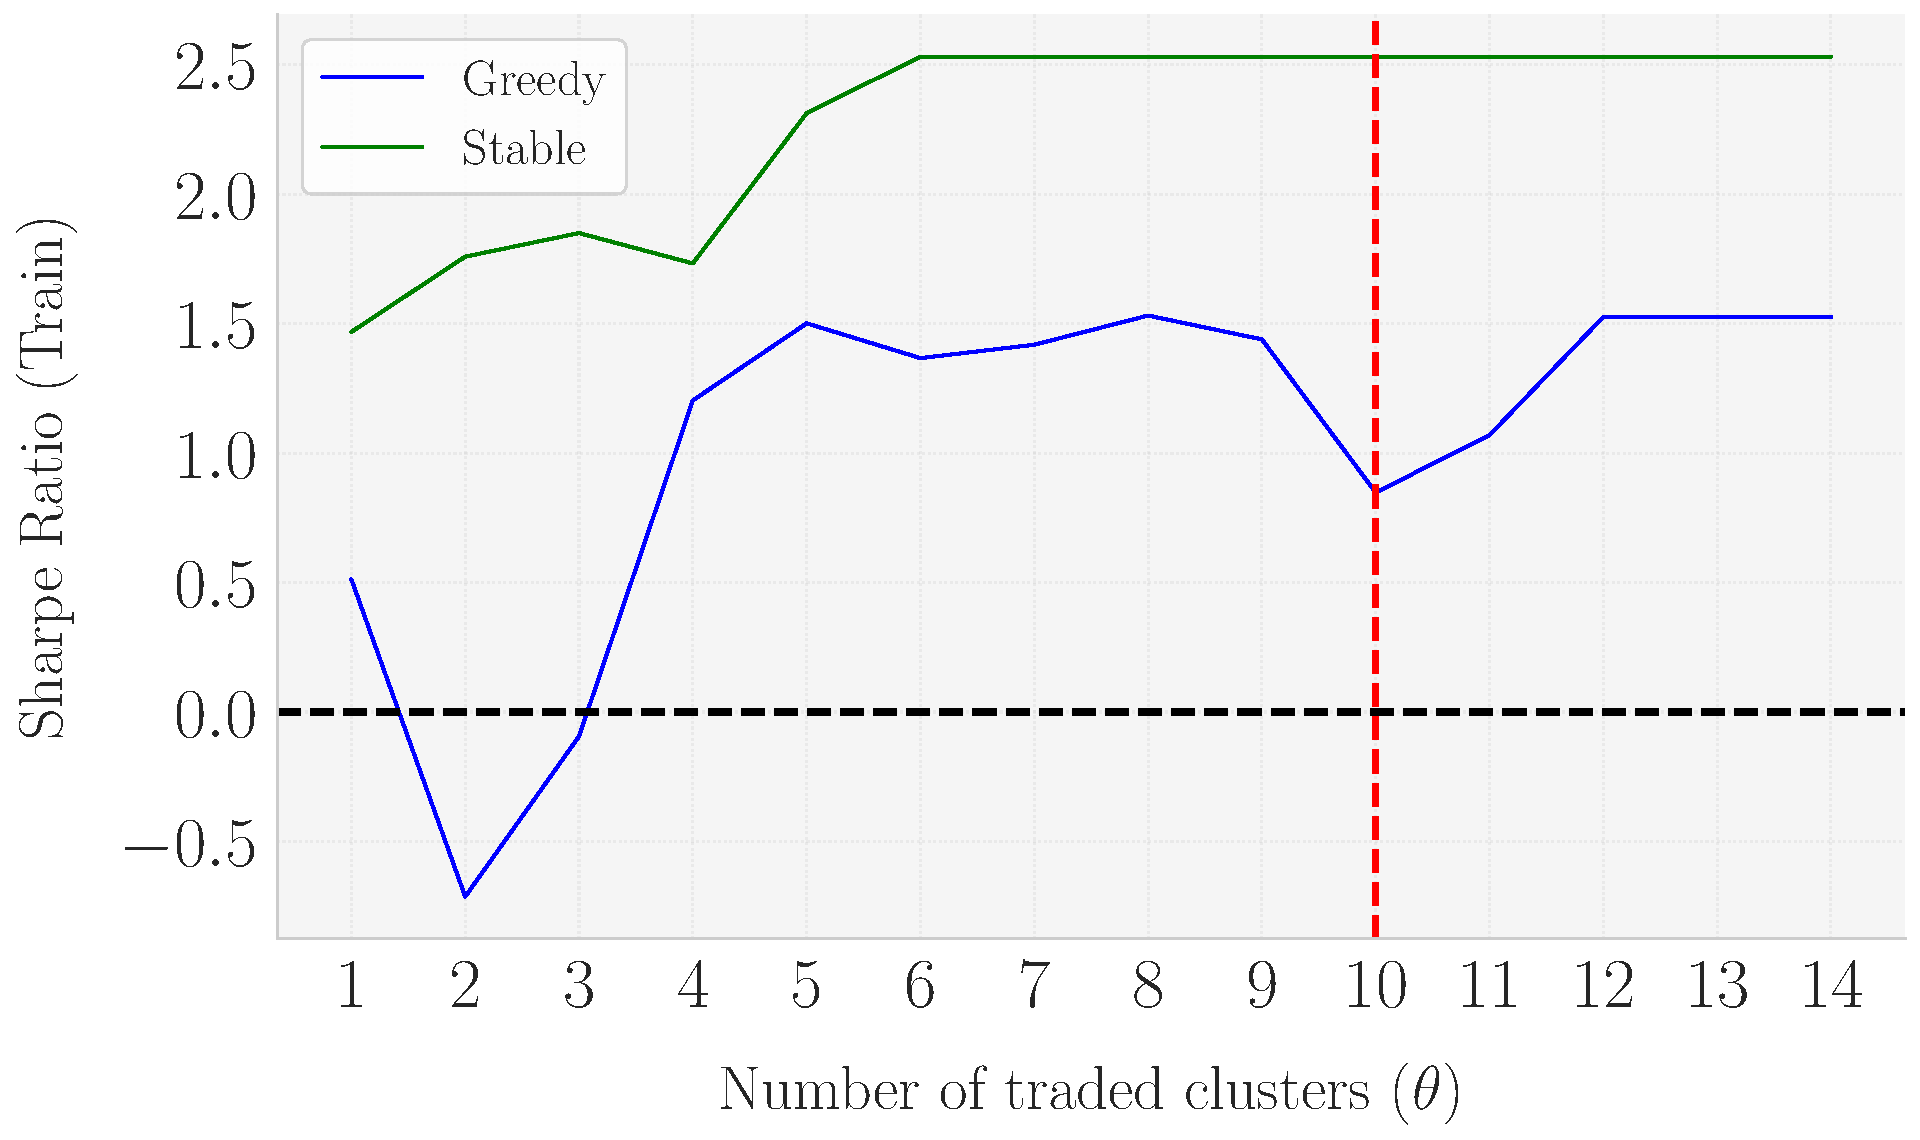
\includegraphics[width=\textwidth]{fig_A4a_LLAMA_SR_Train_vs_theta.pdf}
    \caption{Plot of $SR^{\mathcal P^{tr}}(\theta)$ over a grid of $\theta$}
    \label{fig:LLM_hyp_3}
  \end{subfigure}
  \hspace{0.05\textwidth} % Add horizontal space between the subfigures
  \begin{subfigure}[b]{0.46\textwidth}
    \centering
    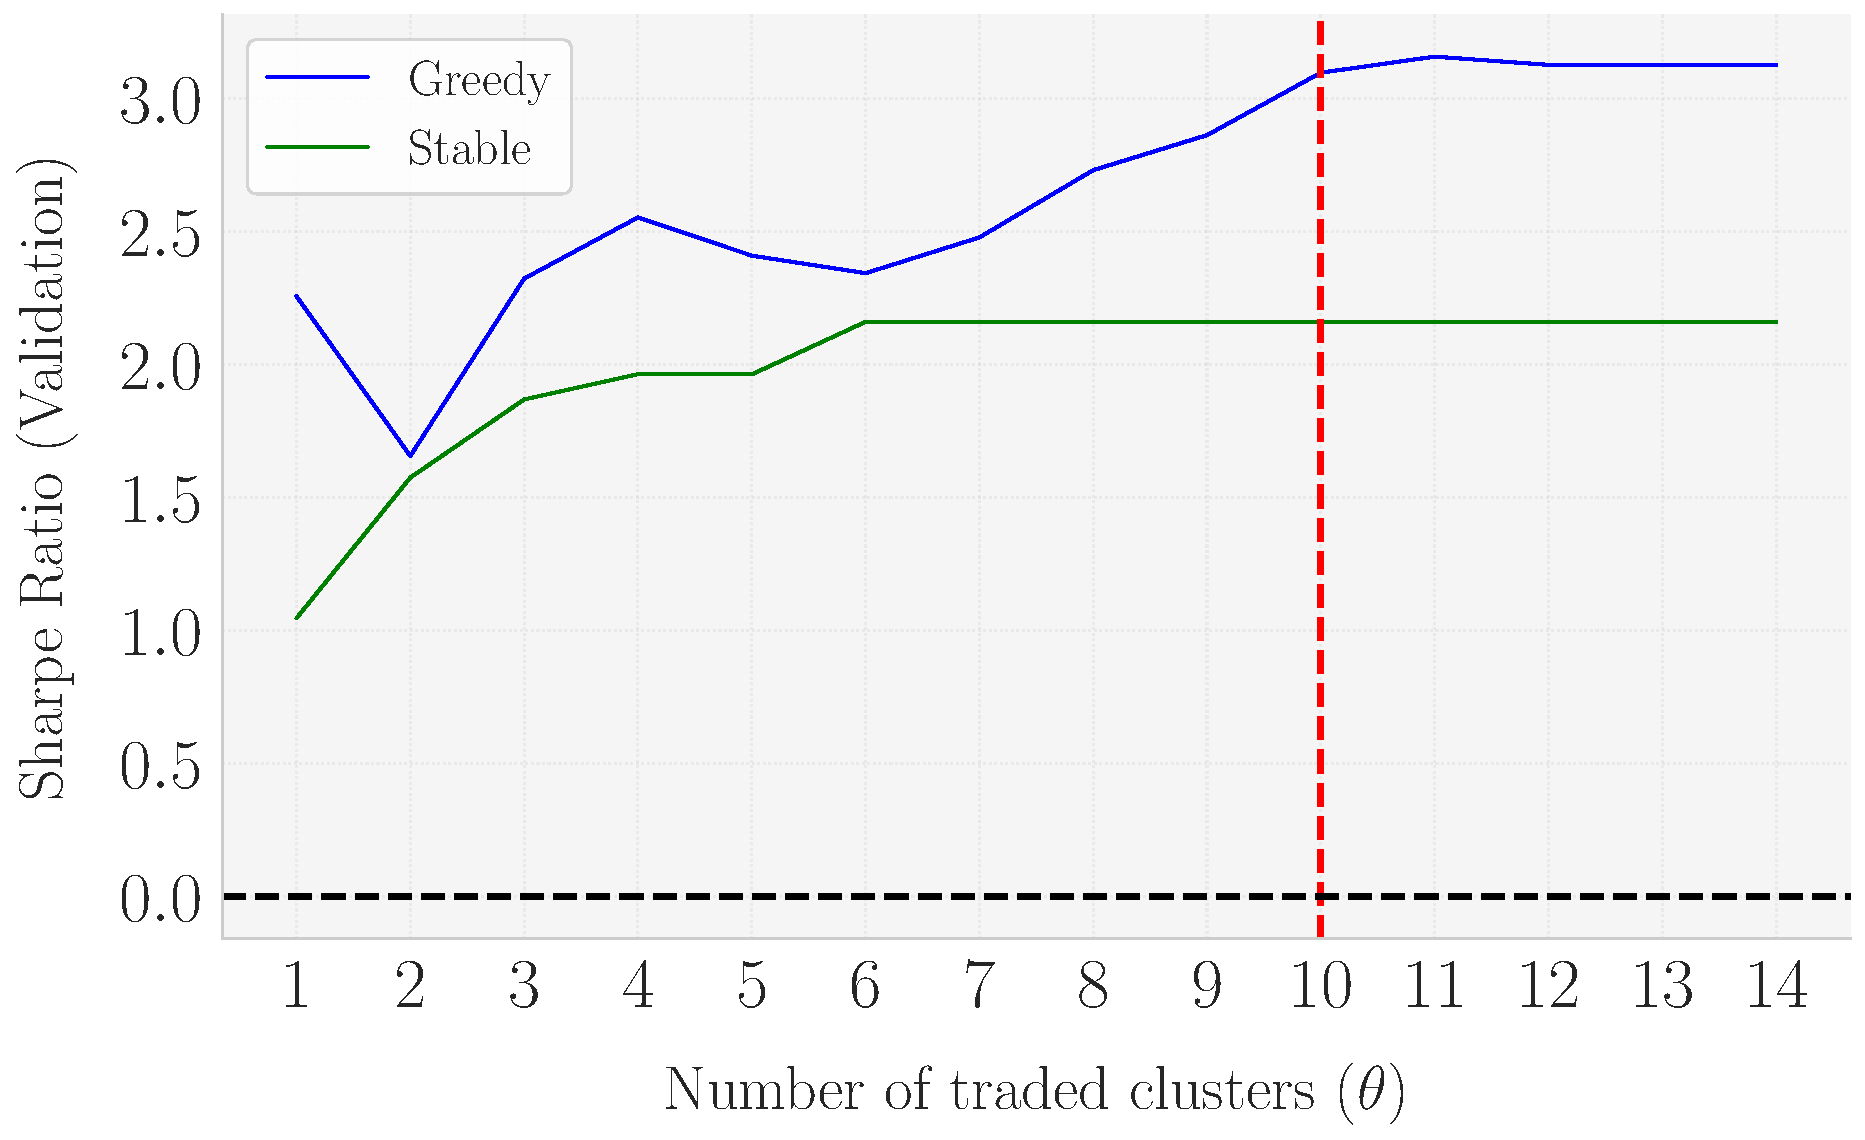
\includegraphics[width=\textwidth]{fig_A4b_LLAMA_SR_Validation_vs_theta.pdf}
    \caption{Plot of $SR^{\mathcal P^{val}}(\theta)$ over a grid of $\theta$}
    \label{fig:LLM_hyp_4}
  \end{subfigure}
\mx
\subcaption*{\textit{Note: This figure illustrates the Sharpe Ratios ($SR$) as a function of $\theta$, the upper bound on the number of traded clusters, for the LLM clustering method in the training (Panel a) and validation (Panel b) splits. In Panel (a), the Sharpe Ratios for the training set indicate a temporary dip at $\theta=10$ for the Greedy algorithm, yet this value still provides a relatively stable outcome. In contrast, Panel (b) shows that $\theta=10$ leads to a noticeable increase in Sharpe Ratios for the validation set, particularly benefiting the Greedy algorithm. The choice of $\theta = \integer{0.5k} = 10$ strikes a balance, confirming it as an effective hyperparameter selection for achieving stability in both the training and validation splits with LLM clustering.}}
\label{fig:LLM_hyperparameter_justification_theta}
\end{figure}
%----------------------------------------------------


%%%%%%%%%%%%%%%%%%%%%%%%%%%%%%%%%%%%%%%%%%%%%%%%%%%%%

\newpage
%%%%%%%%%%%%%%%%%%%%%%%%%%%%%%%%%%%%%%%%%%%%%%%%%%%%%
\subsection{Cluster-Average Sharpe Ratios}
The distribution of cluster-average Sharpe Ratios across different clusters reveals distinct patterns between KMeans and LLM-based clustering approaches, as illustrated in Figure \ref{fig:cluster-average-SR-by-split}

Panel A presents the results for KMeans clustering, where we observe remarkably consistent distributional patterns across all three data splits. The distributions are approximately symmetric around zero, with the majority of Sharpe ratios falling within the [-5, 5] range. The training set exhibits the highest density peak (approximately 0.17), followed closely by the test set, while the validation set shows a slightly lower peak density of about 0.125. Notable in the validation set are small secondary peaks at the tails (around �15), suggesting the presence of a few clusters with extreme performance characteristics. This consistency across splits suggests that the KMeans clustering approach produces stable performance groupings.

Panel B displays the results for LLM-based clustering, revealing more heterogeneous distributions across the splits. The validation set demonstrates a pronounced peak near zero with a maximum density of 0.2, indicating strong concentration of performance in this region. In contrast, the training set exhibits a markedly different pattern, with a flatter, more dispersed distribution extending from -20 to +20, suggesting greater performance variability across clusters. The test set presents an intermediate case, with moderate concentration around zero but maintaining significant mass in the positive region. This heterogeneity across splits might indicate that the LLM-based clustering captures more nuanced and potentially time-varying patterns in the underlying data.

The contrasting patterns between the two clustering approaches suggest different strengths: KMeans provides more stable and consistent performance groupings, while LLM-based clustering potentially captures more complex relationships, albeit with greater variability across different data splits.
%----------------------------------------------------
\inserthere{fig:cluster-average-SR-by-split}

\begin{figure}[htbp]
\caption{Distribution of Cluster-Average Sharpe Ratios $(\overline{SR}_g)$ by Split}
\label{fig:cluster-average-SR-by-split}

\begin{subfigure}[t]{0.49\textwidth}
\caption{Panel A: KMeans Clustering}
\centering
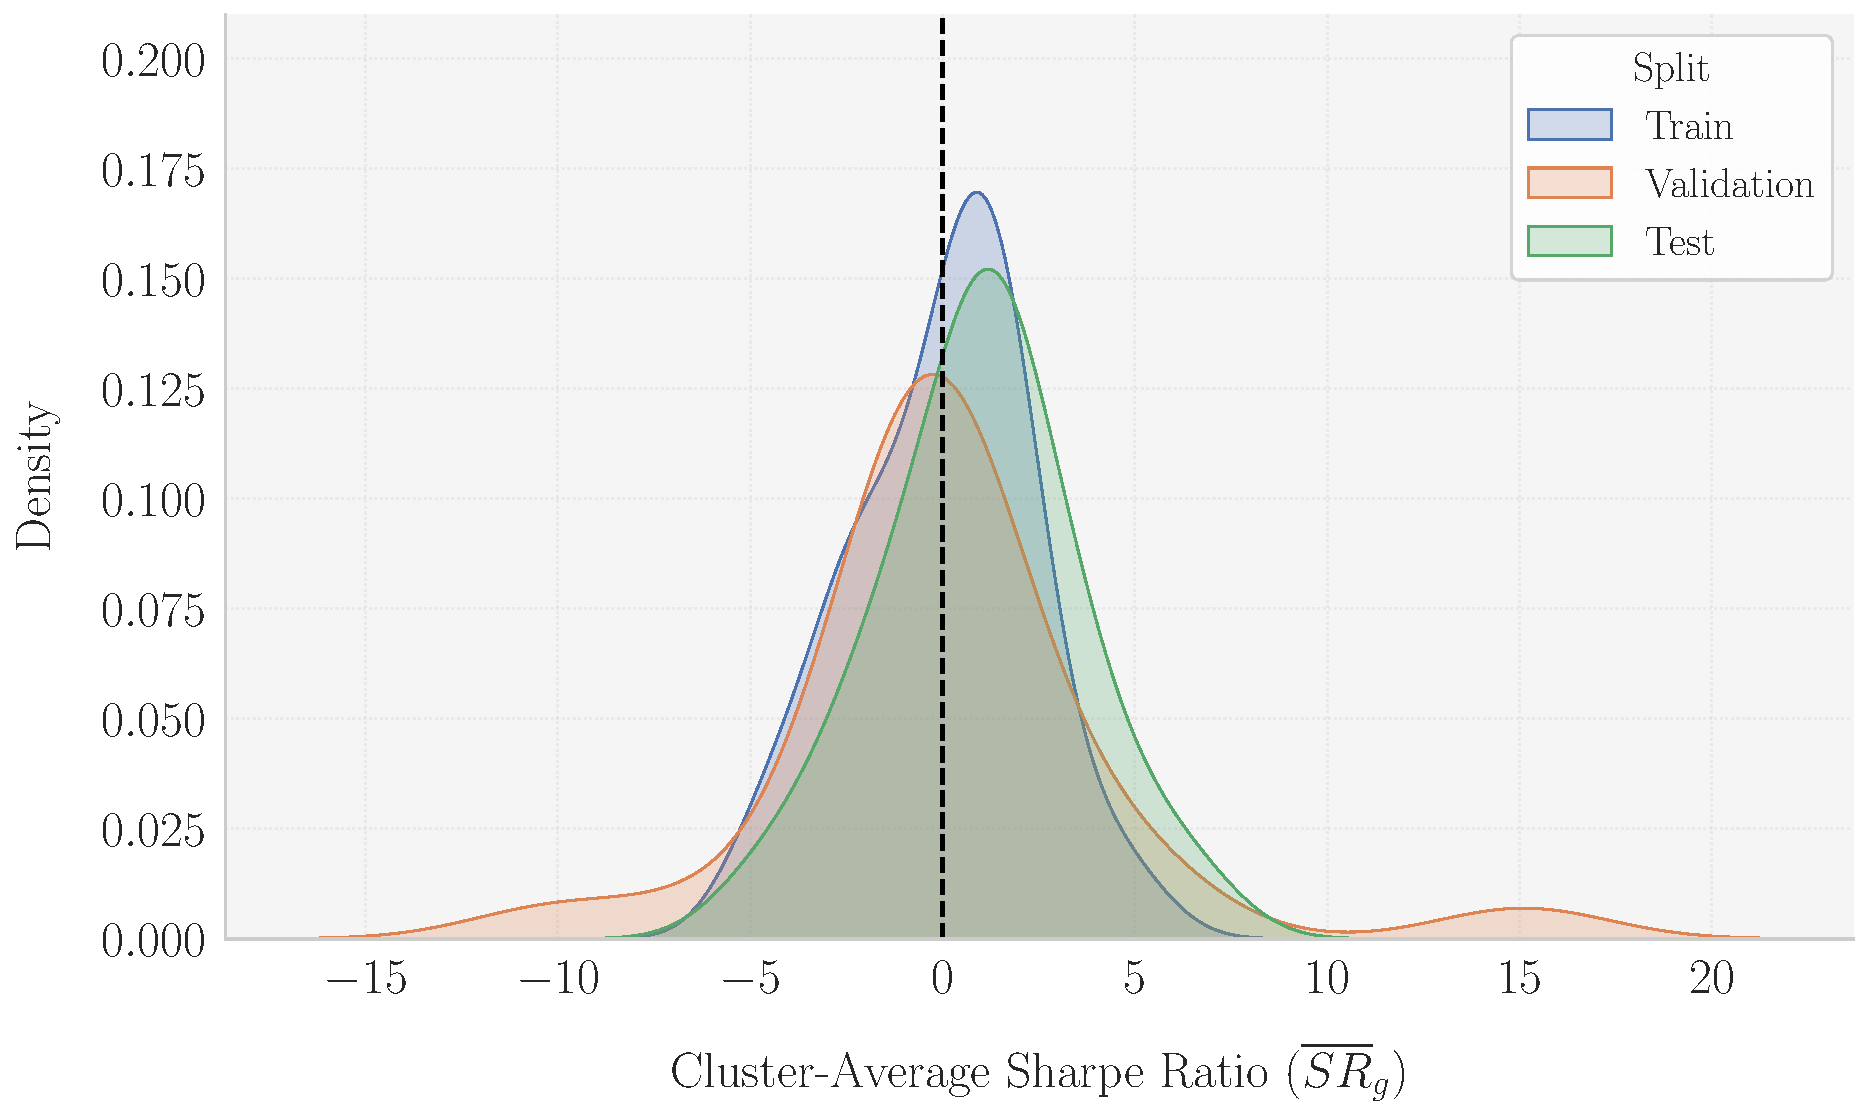
\includegraphics[width=\textwidth]{fig_A5a_KMeans_Cluster-Avg_SR_Distribution.pdf}
\end{subfigure}
\hfill
\begin{subfigure}[t]{0.49\textwidth}
\caption{Panel B: LLM Clustering}
\centering
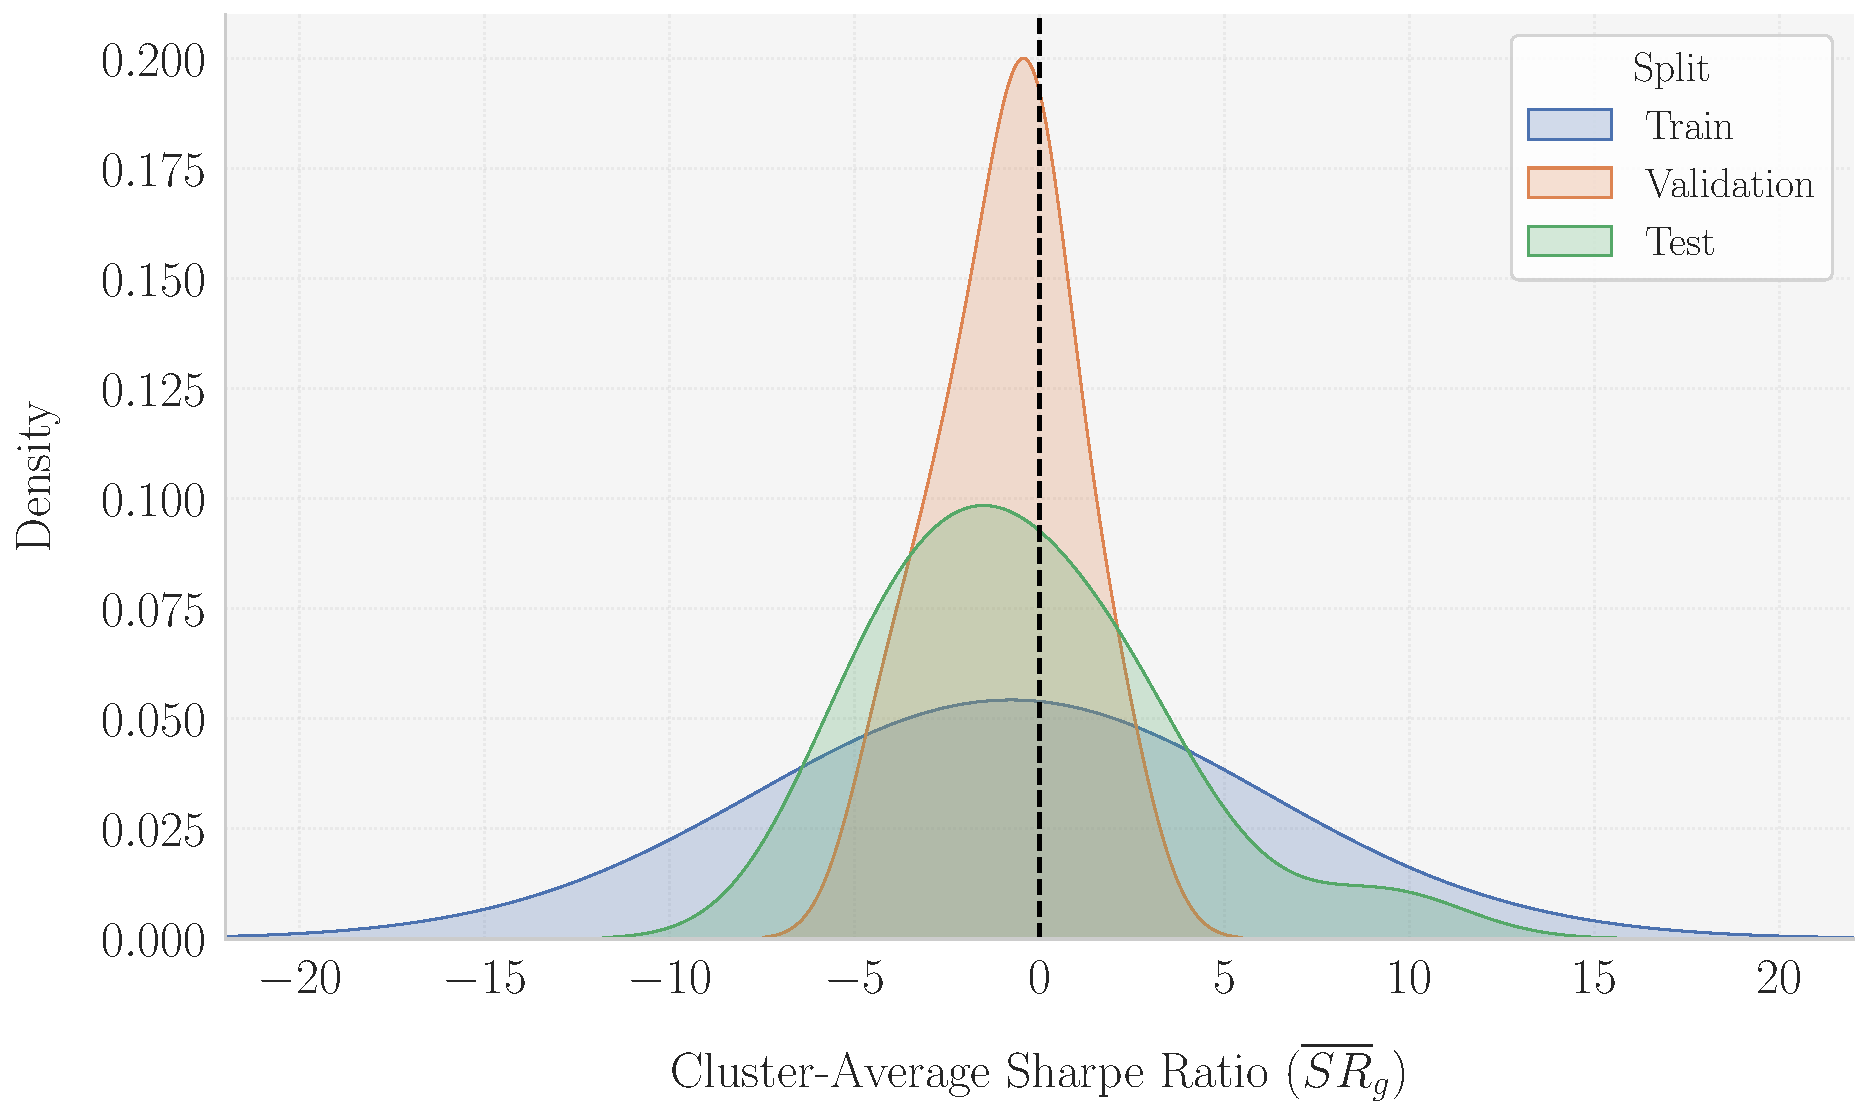
\includegraphics[width=\textwidth]{fig_A5b_LLAMA_Cluster-Avg_SR_Distribution.pdf}
\end{subfigure}

\vspace{0.5cm}
\begin{minipage}{\textwidth}
\setlength{\parindent}{0pt}
{\footnotesize\textit{Note:
This figure presents the distribution of cluster-average Sharpe Ratios $(\overline{SR}_g)$ across training, validation, and test data splits for both KMeans clustering (Panel A) and LLM clustering (Panel B). Each Sharpe Ratio is computed as the average of beta-neutral positions associated with articles in a given cluster. The KMeans approach (Panel A) shows distributions centered around 0 in the validation set, with some outliers exhibiting unusually high or low Sharpe Ratios. The training and test set distributions are slightly right-skewed, suggesting better performance in certain clusters, with no significant outliers. In contrast, the LLM clustering (Panel B) exhibits left-skewed distributions across all splits, indicating a higher frequency of lower Sharpe Ratios. The training data shows fat tails, suggesting extreme values, while the validation data has lighter tails. The test data distribution is more bell-shaped, with Sharpe Ratios concentrated between 5 and 15, indicating stronger performance in some clusters.
}}
\end{minipage}
\end{figure}
%----------------------------------------------------
%%%%%%%%%%%%%%%%%%%%%%%%%%%%%%%%%%%%%%%%%%%%%%%%%%%%%

\newpage
% ptimal Cluster Selection
%%%%%%%%%%%%%%%%%%%%%%%%%%%%%%%%%%%%%%%%%%%%%%%%%%%%%
\subsection{Optimal Cluster Selection Algorithms}
\begin{algorithm}
\caption{
\textsc{Greedy Selection} 
~|~
{{Top average Sharpe Ratio in Validation Set}}
}
%%%%%%%%%%%%%%%%%%%%%%%%%%%%%%%%%%%%%%%%%%%%%%%%%%%%%
\label{alg:greedy_selection}
%%%%%%%%%%%%%%%%%%%%%%%%%%%%%%%%%%%%%%%%%%%%%%%%%%%%%
\begin{algorithmic}[1]
\mx 
\State \textbf{Input:} Set of clusters $\mathcal{G} = \{1, 2, \ldots, k^*\}$, Sharpe Ratios in the validation sample $\{SR_L^{(i,j)}\}_{(i,j)\in \mathcal B^{val}}$, maximum number of traded clusters $\theta\in\mathbb{N}$ (usually, $\theta\propto k^*)$

\mx 
\State \textbf{Output:} Set of long-traded clusters $\mathcal{G}_{\theta}^{+}$ and set of short-traded clusters $\mathcal{G}_{\theta}^{-}$
%----------------------------------------------------
\vspace{0.4cm}
\Statex \underline{\textit{Step \#1: Compute Cluster Average Sharpe Ratios in Validation Set}}
\For{each $g \in \mathcal{G}$}
    \State Compute average Sharpe Ratio ~
$
\overline{S R}_g^{val} \leftarrow \frac{1}{|\mathcal{B}_g^{val} |} \sum_{(i,j) \in \mathcal{B}_g^{val}} S R_{{{L}}}^{(i,j)}
$
\EndFor
%----------------------------------------------------
\vspace{0.4cm}
\Statex \underline{\textit{Step \#2: Identify Positive and Negative Sharpe Ratio Clusters}}
\State Define $\mathcal{G}_{SR^+}^{val} \leftarrow \{ g \in \mathcal{G} \mid \overline{SR}_g^{val} > 0 \}$
\State Define $\mathcal{G}_{SR^-}^{val} \leftarrow \{ g \in \mathcal{G} \mid \overline{SR}_g^{val} < 0 \}$
%----------------------------------------------------
\vspace{0.4cm}
\Statex \underline{\textit{Step \#3: Rank Clusters by Average Sharpe Ratio in the Validation Set}}
\For{each $g \in \mathcal{G}$}
	\State Rank the average Sharpe Ratio~~
$
\mathfrak{R}_g^{val} \leftarrow  \sum_{h \in \mathcal{G}} 
\mathbf{1}\1{
\overline{S R}_h^{val} \geq \overline{S R}_g^{val} 
}
$
\EndFor
%----------------------------------------------------
\vspace{0.4cm}
\Statex \underline{\textit{Step \#4: Select Top $\theta$ Clusters}}
\State Define $\theta^+ \leftarrow \min(\theta, |\mathcal{G}_{SR^+}^{val}|)$
;~~
$\mathcal{G}_{\theta}^{+} \leftarrow \{ g\in\G \mid 1 \leq \mathfrak{R}_g^{val} \leq \theta^+ \}$
%\State 

\State Define $\theta^- \leftarrow \min(\theta, |\mathcal{G}_{SR^-}^{val}|)$
;~~
%\State 
 $\mathcal{G}_{\theta}^{-} \leftarrow \{ g \in\G \mid k^* - \theta^- < \mathfrak{R}_g^{val} \leq k^* \}$
%----------------------------------------------------
\vspace{0.5cm}
\State \textbf{Return} Long-traded clusters $\mathcal{G}_{\theta}^{+}$, Short-traded clusters $\mathcal{G}_{\theta}^{-}$

\end{algorithmic}
\end{algorithm}

\begin{algorithm}[H]
\caption{
\textsc{Rank Stability}
~ |~
{{Minimal Rank Difference between Train \& Validation Sets}
}}
%%%%%%%%%%%%%%%%%%%%%%%%%%%%%%%%%%%%%%%%%%%%%%%%%%%%%
\label{alg:rank_stability}
%%%%%%%%%%%%%%%%%%%%%%%%%%%%%%%%%%%%%%%%%%%%%%%%%%%%%
\begin{algorithmic}[1]
\mx 
\State \textbf{Input:} Set of clusters $\mathcal{G} = \{1, 2, \ldots, k^*\}$, Sharpe Ratios in the training and validation sample $\{SR_L^{(i,j)}\}_{(i,j)\in \mathcal B^{tr}}$ and $\{SR_L^{(i,j)}\}_{(i,j)\in \mathcal B^{val}}$, maximum number of traded clusters $\theta$
\mx 
\State \textbf{Output:} Set of long-traded clusters $\mathcal{G}_{\theta}^{+}$ and set of short-traded clusters $\mathcal{G}_{\theta}^{-}$
%----------------------------------------------------
%\Statex
\mx
\Statex \underline{\textit{Step \#1: Compute Cluster Average Sharpe Ratios in Training \& Validation Set}}
\For{each $g \in \mathcal{G}$}
    \State Compute average Sharpe Ratio in $\mathcal B^{tr}:$ ~~
$
\overline{S R}_g^{tr} \leftarrow \frac{1}{|\mathcal{B}_g^{tr} |} \sum_{(i,j) \in \mathcal{B}_g^{tr}} S R_{{{L}}}^{(i,j)}
$
    \State Compute average Sharpe Ratio in $\mathcal B^{val}:$ ~
$
\overline{S R}_g^{val} \leftarrow \frac{1}{|\mathcal{B}_g^{val} |} \sum_{(i,j) \in \mathcal{B}_g^{val}} S R_{{{L}}}^{(i,j)}
$
\EndFor
%----------------------------------------------------
%\Statex
\mx
\Statex \underline{\textit{Step \#2: Rank Clusters}}
%\State \# \textit{Step 1: Rank Clusters}
\For{each $g \in \mathcal{G}$}
    \State Rank the average Sharpe Ratios in $\mathcal B^{tr}:$ ~~
%$\{\overline{S R}_g^{tr}\}_{g\in\G}$ 
$
\mathfrak{R}_g^{tr} \leftarrow  \sum_{h \in \mathcal{G}} 
\mathbf{1}\1{
\overline{S R}_h^{t r} \geq \overline{S R}_g^{t r} 
}
$
    \State Rank the average Sharpe Ratios in $\mathcal B^{val}:$ ~
%$\{\overline{S R}_g^{tr}\}_{g\in\G}$ 
$
\mathfrak{R}_g^{val} \leftarrow  \sum_{h \in \mathcal{G}} 
\mathbf{1}\1{
\overline{S R}_h^{val} \geq \overline{S R}_g^{val} 
}
$
\EndFor
%----------------------------------------------------
%\Statex
\mx
\Statex \underline{\textit{Step \#3: Calculate Rank Differences}}
\For{each $g \in \mathcal{G}$}
    \State Calculate rank difference $\delta_g \leftarrow | \mathfrak R_g^{tr} - \mathfrak R_g^{val} |$
\EndFor
%----------------------------------------------------
%\Statex
\mx
\Statex \underline{\textit{Step \#4: Select Top $\theta$ Clusters with Smallest Rank Differences}}
\For{each $g \in \mathcal{G}$}
\State Rank the rank difference $:~~ \mathfrak{R}(\delta_g) \leftarrow \sum_{h\in\G} \mbf{1} \1{ \delta_g \geq  \delta_h }$
\EndFor
\State Select top $2\theta$ clusters with smallest $\delta_g$: 
$
~~
\mathcal{G}_{\theta} = 
\3{
g\in\G \c 1 \leq \mathfrak{R}(\delta_g) \leq 2\theta 
}
~
$
%----------------------------------------------------
%\Statex
\mx
\Statex \underline{\# \textit{Step 5: Determine Long and Short Positions}}
\State Define $\mathcal{G}_{\theta}^{+} = \{g \in \mathcal{G}_{\theta} \mid \overline{SR}_g^{tr} > 0 \text{ and } \overline{SR}_g^{val} > 0\}$
\State Define $\mathcal{G}_{\theta}^{-} = \{g \in \mathcal{G}_{\theta} \mid \overline{SR}_g^{tr} < 0 \text{ and } \overline{SR}_g^{val} < 0\}$
%----------------------------------------------------
%\Statex
\mx
\State \textbf{Return} Long-traded clusters $\mathcal{G}_{\theta}^{+}$, Short-traded clusters $\mathcal{G}_{\theta}^{-}$

\end{algorithmic}
\end{algorithm}


%%%%%%%%%%%%%%%%%%%%%%%%%%%%%%%%%%%%%%%%%%%%%%%%%%%%%

% Sample of articles for each cluster
%%%%%%%%%%%%%%%%%%%%%%%%%%%%%%%%%%%%%%%%%%%%%%%%%%%%%
\subsection{Sample of articles for each cluster}
\setcounter{table}{0}
\renewcommand{\thetable}{A\arabic{table}} % To ensure the tables in the appendix are numbered as A1, A2, etc.
%%%%%%%%%%%%%%%%%%%%%%%%%%%%%%%%%%%%%%%%%%%%%%%%%%%%%
%%%%%%%%%%%%%% 		ENGLISH 		%%%%%%%%%%%%%%%%%
%%%%%%%%%%%%%%%%%%%%%%%%%%%%%%%%%%%%%%%%%%%%%%%%%%%%%
%%%%%%%%%%%%%%%%%%%%%%%%%%%%%%%%%%%%%%%%%%%%%%%%%%%%%

\begin{landscape}
\renewcommand{\arraystretch}{1}

%\scriptsize
{\fontsize{9}{9}\selectfont % Set custom font size between \scriptsize and \tiny

%----------------------------------------------------
\begin{longtable}{|c|L{8cm}|L{14cm}|}
\caption{KMeans clustering. Proposed name for the clusters and sample of 3 articles for each cluster.} % Caption for the longtable
\label{tab:KMeans_Articles_3_English} \\
\hline 
\rowcolor{lightgray}
\# & \multicolumn{1}{c|}{Title} & \multicolumn{1}{c|}{Articles} \\
\hline \hline 
0 
& 
Miscellaneous (Colonial, Acciona, Amadeus, Grifols, Endesa, IAG, Bankinter...)
& 
\textbullet~Colonial forecasts rental income of EUR338m in 2020

\textbullet~Acciona's asset sales will allow it to grow in renewables

\textbullet~Sabadell recommends selling Amadeus shares due to worse sales forecast.
\\ \hline 
1
& 
Quarterly \& Semi-Annual Earnings Reports
& 
\textbullet~Enag�s 1H net profit falls 9.8\% due to lower income and extraordinary items.

\textbullet~Iberdrola: Net profit of EUR1.025m in Q1

\textbullet~Santander almost quintuples Q1 profit due to absence of Covid provisions.
\\ \hline 
2
& 
BBVA \& Sabadell: Financial Performance \& Strategic Movements
& 
\textbullet~Interest rate hike in Turkey favors BBVA's net interest margin

\textbullet~Sabadell reorganizes business in Spain following the arrival of the new CEO.

\textbullet~Fitch downgrades Banco Sabadell's rating one notch to low grade.
\\ \hline 
3
& 
Telef�nica \& Cellnex: Telecommunications Tower Sales \& Market Dynamics
& 
\textbullet~Telef�nica shares soar after selling towers of its subsidiary in Europe and Latin America.

\textbullet~Telef�nica hires Goldman Sachs to sell its British tower business

\textbullet~Dutch Competition Authority authorizes Cellnex to integrate 3,150 Deutsche Telekom towers.
\\ \hline 
4
& 
CaixaBank: Mergers and Strategic Moves in the Banking Sector
& 
\textbullet~CaixaBank and Bankia approve their merger project

\textbullet~CaixaBank closes its first issuance of green bonds in pounds for 500 million

\textbullet~CaixaBank-Bankia merger could generate EUR500m in savings
\\ \hline 
5
& 
Telef�nica, Indra, \& M�sM�vil: Regulatory and Strategic Moves in Telecom
& 
\textbullet~Indra to partner with Telef�nica in the deployment of fiber optics in Germany.

\textbullet~Telef�nica launches a buyback offer for its hybrid bonds of EUR1.000m.

\textbullet~EU refers Liberty Global and Telef�nica agreement to UK regulator
\\ \hline 
6
& 
Siemens Gamesa: Supply Agreements, Profitability Targets in Renewable Energy
& 
\textbullet~Siemens Gamesa will supply turbines to Elawan's 150 MW wind farm in Spain.

\textbullet~Siemens Gamesa lowers its profitability target for 2021.

\textbullet~Siemens Gamesa will supply 160 MW for the largest wind farm in the Philippines.
\\ \hline 
7
& 
Cellnex: Strategic Acquisitions and Financial Moves in Telecom Infrastructure
& 
\textbullet~Cellnex launches a EUR1.850m debt issue

\textbullet~Cellnex agrees to buy 10,500 telecommunications towers in France for EUR5.200m

\textbullet~Benetton family sells 2.5\% of Cellnex to Singapore sovereign fund
\\ \hline 
8
& 
Acciona, Endesa, Enag�s \& Naturgy: Strategic Moves \& Regulatory Developments in the Energy Sector
& 
\textbullet~Naturgy and Enag�s study project to produce green hydrogen in Asturias

\textbullet~Break of ties between Algeria and Morocco may damage gas flow to Spain

\textbullet~Acciona: Energy business IPO on track for 1H
\\ \hline 
9
& 
Repsol: Strategic Moves and Challenges in the Energy Sector
& 
\textbullet~Repsol to produce green hydrogen at Petronor refinery in 2022

\textbullet~Repsol and Talgo to jointly promote the creation of renewable hydrogen trains

\textbullet~Repsol gains access to a portfolio of renewable assets in Chile through a joint venture
\\ \hline 
10
& 
Ferrovial, Acciona: Strategic Expansions and Financial Maneuvers in Infrastructure
& 
\textbullet~Ferrovial closes the sale of Broadspectrum to Ventia for EUR291m

\textbullet~Acciona awarded the construction of 2 roads in Poland for EUR642m

\textbullet~Renfe awards on-board services contract to Ferrovial for EUR272m
\\ \hline 
11
& 
Solaria: Strategic Moves and Market Challenges in Renewable Energy
& 
\textbullet~Solaria invests EUR220m in Europe's largest photovoltaic park.

\textbullet~Solaria will supply energy to Shell and Axpo with Europe's largest photovoltaic plant

\textbullet~Goldman Sachs downgrades Solaria recommendation after stock rise.
\\ \hline 
12
& 
Iberdrola: Strategic Collaborations and Renewable Energy Developments
& 
\textbullet~Iberdrola will build a self-consumption plant for Lactalis factory in Spain.

\textbullet~Iberdrola and Mapfre launch a renewable energy co-investment vehicle in Spain.

\textbullet~Iberdrola partners with Mitsubishi to decarbonize the industry.
\\ \hline 
13
& 
IAG: Financial Performance
& 
\textbullet~IAG Q3 results worse than expected

\textbullet~IAG burns cash faster than anticipated

\textbullet~IAG stock may be pricing in a second capital increase
\\ \hline 
14
& 
Santander \& CaixaBank: Financial Moves and Sustainability Initiatives 
& 
\textbullet~CaixaBank mobilizes EUR12.000m in sustainable financing in the first 9 months of 2020.

\textbullet~EIB and Banco Santander will inject EUR587m into Portuguese SMEs.

\textbullet~Banco Santander, leader in renewable project financing in 2020.
\\ \hline 
15
& 
ACS \& Acciona: Strategic Movements and Infrastructure Projects
& 
\textbullet~ACS and Acciona win contracts for new Australian airport worth EUR164m.

\textbullet~Acciona awarded 3 contracts to operate wastewater treatment plants in Sardinia for EUR210m.

\textbullet~ACS expects net profit to grow by around 30\% in 2021
\\ \hline 
16
& 
Telef�nica: Financial Performance and Strategic Moves
& 
\textbullet~Reduction in Telef�nica's debt will improve analysts' perception

\textbullet~Telef�nica's profit more than doubles in Q1 due to lower financial expenses.

\textbullet~Telef�nica, Am�rica M�vil and TIM buy the mobile network of Brazil's Oi.
\\ \hline 
17
& 
Meli� and Spanish Tourism Sector: Challenges Amidst the Pandemic
& 
\textbullet~Meli�: Spanish hotel sector faces another uncertain summer with cautious optimism.

\textbullet~Meli� claims EUR116m from the Spanish government for pandemic-related damages.

\textbullet~Meli�: Local Covid-19 lockdowns will continue to affect Meli�.
\\ \hline 
18
& 
Takeover Bids for Naturgy and M�sM�vil
& 
\textbullet~Australian fund IFM launches EUR5.000m bid for 22.69\% of Naturgy.

\textbullet~Polygon fund asks CNMV to review and alter the bid for M�sM�vil.

\textbullet~IFM accepts Spanish government conditions in partial bid for Naturgy.
\\ \hline 
19
& 
Naturgy: Financial Performance
& 
\textbullet~Naturgy presents "weak" 2020 results

\textbullet~Naturgy may revise its strategic plan upwards due to gas prices.

\textbullet~Bank of America sees upside potential for Naturgy based on fundamentals.
\\ \hline 
20
& 
PharmaMar, Grifols: Regulatory Approvals and Market Moves in the Pharmaceutical Sector
& 
\textbullet~EU court annuls European Commission's refusal to market PharmaMar drug.

\textbullet~Grifols starts issuing EUR2.000m bonds to buy Biotest.

\textbullet~PharmaMar announces approval of lurbinectedin for lung cancer in Australia.
\\ \hline 
21
& 
Repsol: Financial Performance
& 
\textbullet~Repsol: Net loss of EUR3.289m in 2020.

\textbullet~Repsol reports a loss of EUR711m in Q4 due to exploration and production provisions

\textbullet~Repsol posts a loss of EUR94m in Q3 due to provisions and lower refining margins.
\\ \hline 
22
& 
Aena: Financial Performance
& 
\textbullet~JPMorgan raises Aena's target price to EUR155 from EUR135.

\textbullet~Aena risks a revenue cut of up to EUR2.000m due to rents.

\textbullet~Aena loses EUR170.7m in 1H as passenger traffic plummets due to the pandemic.
\\ \hline 
23
& 
Enag�s, Endesa, Iberdrola, Red El�ctrica: Regulatory and Market Challenges in the Energy Sector
& 
\textbullet~Spanish electric utilities will remain under pressure in the stock market 

\textbullet~Spanish government measures are bad news for the electric sector.

\textbullet~Spain's electricity price closes February with a 52\% drop vs January
\\ \hline 
24
& 
BBVA, CaixaBank, Banco Sabadell: Layoffs and Restructuring
& 
\textbullet~CaixaBank proposes to unions a redundancy plan affecting 8,291 employees.

\textbullet~Banco Santander closes its redundancy plan with 3,572 voluntary exits and 19 dismissals 

\textbullet~Sabadell prepares an adjustment plan affecting 2,000 employees
\\ \hline 
25
& 
Inditex, Acerinox: Market Performance and Strategic Developments in the Post-Covid Context
& 
\textbullet~Inditex reopens 94\% of its stores worldwide after Covid-19 pandemic.

\textbullet~Sale of Nippon Steel in Acerinox is negative, but expected.

\textbullet~Inditex stock already prices in a strong business recovery.
\\ \hline 
\end{longtable}
%----------------------------------------------------
}

\end{landscape}


%%%%%%%%%%%%%%%%%%%%%%%%%%%%%%%%%%%%%%%%%%%%%%%%%%%%%%
%%%%%%%%%%%%%%%%%%%%%%%%%%%%%%%%%%%%%%%%%%%%%%%%%%%%%%
%%%%%%%%%%%%%%% 		ENGLISH 		%%%%%%%%%%%%%%%%%
%%%%%%%%%%%%%%%%%%%%%%%%%%%%%%%%%%%%%%%%%%%%%%%%%%%%%%
%%%%%%%%%%%%%%%%%%%%%%%%%%%%%%%%%%%%%%%%%%%%%%%%%%%%%%
%
%\begin{landscape}
%\renewcommand{\arraystretch}{1}
%
%
%%\scriptsize
%{\fontsize{9}{9}\selectfont % Set custom font size between \scriptsize and \tiny
%
%
%
%%----------------------------------------------------
%\begin{longtable}{|c|L{8cm}|L{14cm}|}
%\caption{KMeans clustering. Proposed name for the clusters and sample of 3 articles for each cluster.} \\ % Caption for the longtable
%\hline 
%\rowcolor{lightgray}
%\# & \multicolumn{1}{c|}{Title} & \multicolumn{1}{c|}{Articles} \\
%\hline \hline 
%0 
%& 
%Miscellaneous (Colonial, Acciona, Amadeus, Grifols, Endesa, IAG, Bankinter...)
%& 
%\textbullet~Colonial forecasts rental income of EUR338m in 2020
%
%\textbullet~Acciona's asset sales will allow it to grow in renewables
%
%\textbullet~Sabadell recommends selling Amadeus shares due to worse sales forecast.
%\\ \hline 
%1
%& 
%Quarterly \& Semi-Annual Earnings Reports
%& 
%\textbullet~Enag�s 1H net profit falls 9.8\% due to lower income and extraordinary items.
%
%\textbullet~Iberdrola: Net profit of EUR1.025m in Q1
%
%\textbullet~Santander almost quintuples Q1 profit due to absence of Covid provisions.
%\\ \hline 
%2
%& 
%BBVA \& Sabadell: Financial Performance \& Strategic Movements
%& 
%\textbullet~Interest rate hike in Turkey favors BBVA's net interest margin
%
%\textbullet~Sabadell reorganizes business in Spain following the arrival of the new CEO.
%
%\textbullet~Fitch downgrades Banco Sabadell's rating one notch to low grade.
%\\ \hline 
%3
%& 
%Telef�nica \& Cellnex: Telecommunications Tower Sales \& Market Dynamics
%& 
%\textbullet~Telef�nica shares soar after selling towers of its subsidiary in Europe and Latin America.
%
%\textbullet~Telef�nica hires Goldman Sachs to sell its British tower business
%
%\textbullet~Dutch Competition Authority authorizes Cellnex to integrate 3,150 Deutsche Telekom towers.
%\\ \hline 
%4
%& 
%CaixaBank: Mergers and Strategic Moves in the Banking Sector
%& 
%\textbullet~CaixaBank and Bankia approve their merger project
%
%\textbullet~CaixaBank closes its first issuance of green bonds in pounds for 500 million
%
%\textbullet~CaixaBank-Bankia merger could generate EUR500m in savings
%\\ \hline 
%5
%& 
%Telef�nica, Indra, \& M�sM�vil: Regulatory and Strategic Moves in Telecom
%& 
%\textbullet~Indra to partner with Telef�nica in the deployment of fiber optics in Germany.
%
%\textbullet~Telef�nica launches a buyback offer for its hybrid bonds of EUR1.000m.
%
%\textbullet~EU refers Liberty Global and Telef�nica agreement to UK regulator
%\\ \hline 
%6
%& 
%Siemens Gamesa: Supply Agreements, Profitability Targets in Renewable Energy
%& 
%\textbullet~Siemens Gamesa will supply turbines to Elawan's 150 MW wind farm in Spain.
%
%\textbullet~Siemens Gamesa lowers its profitability target for 2021.
%
%\textbullet~Siemens Gamesa will supply 160 MW for the largest wind farm in the Philippines.
%\\ \hline 
%7
%& 
%Cellnex: Strategic Acquisitions and Financial Moves in Telecom Infrastructure
%& 
%\textbullet~Cellnex launches a EUR1.850m debt issue
%
%\textbullet~Cellnex agrees to buy 10,500 telecommunications towers in France for EUR5.200m
%
%\textbullet~Benetton family sells 2.5\% of Cellnex to Singapore sovereign fund
%\\ \hline 
%8
%& 
%Acciona, Endesa, Enag�s \& Naturgy: Strategic Moves \& Regulatory Developments in the Energy Sector
%& 
%\textbullet~Naturgy and Enag�s study project to produce green hydrogen in Asturias
%
%\textbullet~Break of ties between Algeria and Morocco may damage gas flow to Spain
%
%\textbullet~Acciona: Energy business IPO on track for 1H
%\\ \hline 
%9
%& 
%Repsol: Strategic Moves and Challenges in the Energy Sector
%& 
%\textbullet~Repsol to produce green hydrogen at Petronor refinery in 2022
%
%\textbullet~Repsol and Talgo to jointly promote the creation of renewable hydrogen trains
%
%\textbullet~Repsol gains access to a portfolio of renewable assets in Chile through a joint venture
%\\ \hline 
%10
%& 
%Ferrovial, Acciona: Strategic Expansions and Financial Maneuvers in Infrastructure
%& 
%\textbullet~Ferrovial closes the sale of Broadspectrum to Ventia for EUR291m
%
%\textbullet~Acciona awarded the construction of 2 roads in Poland for EUR642m
%
%\textbullet~Renfe awards on-board services contract to Ferrovial for EUR272m
%\\ \hline 
%11
%& 
%Solaria: Strategic Moves and Market Challenges in Renewable Energy
%& 
%\textbullet~Solaria invests EUR220m in Europe's largest photovoltaic park.
%
%\textbullet~Solaria will supply energy to Shell and Axpo with Europe's largest photovoltaic plant
%
%\textbullet~Goldman Sachs downgrades Solaria recommendation after stock rise.
%\\ \hline 
%12
%& 
%Iberdrola: Strategic Collaborations and Renewable Energy Developments
%& 
%\textbullet~Iberdrola will build a self-consumption plant for Lactalis factory in Spain.
%
%\textbullet~Iberdrola and Mapfre launch a renewable energy co-investment vehicle in Spain.
%
%\textbullet~Iberdrola partners with Mitsubishi to decarbonize the industry.
%\\ \hline 
%13
%& 
%IAG: Financial Performance
%& 
%\textbullet~IAG Q3 results worse than expected
%
%\textbullet~IAG burns cash faster than anticipated
%
%\textbullet~IAG stock may be pricing in a second capital increase
%\\ \hline 
%14
%& 
%Santander \& CaixaBank: Financial Moves and Sustainability Initiatives 
%& 
%\textbullet~CaixaBank mobilizes EUR12.000m in sustainable financing in the first 9 months of 2020.
%
%\textbullet~EIB and Banco Santander will inject EUR587m into Portuguese SMEs.
%
%\textbullet~Banco Santander, leader in renewable project financing in 2020.
%\\ \hline 
%15
%& 
%ACS \& Acciona: Strategic Movements and Infrastructure Projects
%& 
%\textbullet~ACS and Acciona win contracts for new Australian airport worth EUR164m.
%
%\textbullet~Acciona awarded 3 contracts to operate wastewater treatment plants in Sardinia for EUR210m.
%
%\textbullet~ACS expects net profit to grow by around 30\% in 2021
%\\ \hline 
%16
%& 
%Telef�nica: Financial Performance and Strategic Moves
%& 
%\textbullet~Reduction in Telef�nica's debt will improve analysts' perception
%
%\textbullet~Telef�nica's profit more than doubles in Q1 due to lower financial expenses.
%
%\textbullet~Telef�nica, Am�rica M�vil and TIM buy the mobile network of Brazil's Oi.
%\\ \hline 
%17
%& 
%Meli� and Spanish Tourism Sector: Challenges Amidst the Pandemic
%& 
%\textbullet~Meli�: Spanish hotel sector faces another uncertain summer with cautious optimism.
%
%\textbullet~Meli� claims EUR116m from the Spanish government for pandemic-related damages.
%
%\textbullet~Meli�: Local Covid-19 lockdowns will continue to affect Meli�.
%\\ \hline 
%18
%& 
%Takeover Bids for Naturgy and M�sM�vil
%& 
%\textbullet~Australian fund IFM launches EUR5.000m bid for 22.69\% of Naturgy.
%
%\textbullet~Polygon fund asks CNMV to review and alter the bid for M�sM�vil.
%
%\textbullet~IFM accepts Spanish government conditions in partial bid for Naturgy.
%\\ \hline 
%19
%& 
%Naturgy: Financial Performance
%& 
%\textbullet~Naturgy presents "weak" 2020 results
%
%\textbullet~Naturgy may revise its strategic plan upwards due to gas prices.
%
%\textbullet~Bank of America sees upside potential for Naturgy based on fundamentals.
%\\ \hline 
%20
%& 
%PharmaMar, Grifols: Regulatory Approvals and Market Moves in the Pharmaceutical Sector
%& 
%\textbullet~EU court annuls European Commission's refusal to market PharmaMar drug.
%
%\textbullet~Grifols starts issuing EUR2.000m bonds to buy Biotest.
%
%\textbullet~PharmaMar announces approval of lurbinectedin for lung cancer in Australia.
%\\ \hline 
%21
%& 
%Repsol: Financial Performance
%& 
%\textbullet~Repsol: Net loss of EUR3.289m in 2020.
%
%\textbullet~Repsol reports a loss of EUR711m in Q4 due to exploration and production provisions
%
%\textbullet~Repsol posts a loss of EUR94m in Q3 due to provisions and lower refining margins.
%\\ \hline 
%22
%& 
%Aena: Financial Performance
%& 
%\textbullet~JPMorgan raises Aena's target price to EUR155 from EUR135.
%
%\textbullet~Aena risks a revenue cut of up to EUR2.000m due to rents.
%
%\textbullet~Aena loses EUR170.7m in 1H as passenger traffic plummets due to the pandemic.
%\\ \hline 
%23
%& 
%Enag�s, Endesa, Iberdrola, Red El�ctrica: Regulatory and Market Challenges in the Energy Sector
%& 
%\textbullet~Spanish electric utilities will remain under pressure in the stock market 
%
%\textbullet~Spanish government measures are bad news for the electric sector.
%
%\textbullet~Spain's electricity price closes February with a 52\% drop vs January
%\\ \hline 
%24
%& 
%BBVA, CaixaBank, Banco Sabadell: Layoffs and Restructuring
%& 
%\textbullet~CaixaBank proposes to unions a redundancy plan affecting 8,291 employees.
%
%\textbullet~Banco Santander closes its redundancy plan with 3,572 voluntary exits and 19 dismissals 
%
%\textbullet~Sabadell prepares an adjustment plan affecting 2,000 employees
%\\ \hline 
%25
%& 
%Inditex, Acerinox: Market Performance and Strategic Developments in the Post-Covid Context
%& 
%\textbullet~Inditex reopens 94\% of its stores worldwide after Covid-19 pandemic.
%
%\textbullet~Sale of Nippon Steel in Acerinox is negative, but expected.
%
%\textbullet~Inditex stock already prices in a strong business recovery.
%\\ \hline 
%\end{longtable}
%%----------------------------------------------------
%}
%
%\end{landscape}

%%%%%%%%%%%%%%%%%%%%%%%%%%%%%%%%%%%%%%%%%%%%%%%%%%%%%
%%%%%%%%%%%%%%%%%%%%%%%%%%%%%%%%%%%%%%%%%%%%%%%%%%%%%
%%%%%%%%%%%%%% 3 ARTICLES PER CLUSTER %%%%%%%%%%%%%%%
%%%%%%%%%%%%%%%%%%%%%%%%%%%%%%%%%%%%%%%%%%%%%%%%%%%%%
%%%%%%%%%%%%%%%%%%%%% ENGLISH %%%%%%%%%%%%%%%%%%%%%%%
%%%%%%%%%%%%%%%%%%%%%%%%%%%%%%%%%%%%%%%%%%%%%%%%%%%%%
%%%%%%%%%%%%%%%%%%%%%%%%%%%%%%%%%%%%%%%%%%%%%%%%%%%%%

\begin{landscape}
\renewcommand{\arraystretch}{1}


%\scriptsize
{\fontsize{10}{10}\selectfont % Set custom font size between \scriptsize and \tiny


%----------------------------------------------------
\begin{longtable}{|c|L{8cm}|L{14cm}|}
\caption{LLM clustering. Sample of 3 articles for each cluster.} 
\label{tab:LLM_Articles_3_English} \\
\hline 
\rowcolor{lightgray}
\# & \multicolumn{1}{c|}{Title} & \multicolumn{1}{c|}{Articles} \\
\hline \hline 
0 
& 
Demand, Minor, Positive
& 
\textbullet~Meli�'s recovery will be fast, but it will not be completed until 2023

\textbullet~Tourism sector aid in Spain will have a limited impact on listed companies

\textbullet~Spanish airports will recover pre-pandemic traffic by the end of 2025
\\ \hline 
1
& 
Demand, Minor, Negative
& 
\textbullet~Tallgrass will contribute fewer dividends to Enag�s -JPMorgan Cazenove

\textbullet~Aena's stock decline is due to sector visibility -Sabadell

\textbullet~ObservaTUR believes Spain's economic situation will worsen and calls for more measures
\\ \hline 
2
& 
Demand, Major, Positive
& 
\textbullet~Solaria invests EUR220m in Europe's largest photovoltaic park

\textbullet~Acciona will build Sao Paulo metro line for EUR2.3 billion

\textbullet~Inditex returns to profit in H1 and continues to recover from the pandemic
\\ \hline 
3
& 
Demand, Major, Negative
& 
\textbullet~Passenger traffic at Aena airports falls 79.9\% year-on-year in September

\textbullet~UPDATE: Naturgy's net profit falls 45.6\% in 9m due to Covid-19 impact

\textbullet~Possible capital increase by IAG already priced in
\\ \hline 
4
& 
Supply, Minor, Positive
& 
\textbullet~Repsol returns to profit in Q2 due to crude price increase

\textbullet~Naturgy receives LNG supply contract for ships for 2 years in Spain

\textbullet~Acciona Energ�a starts up 238 MW photovoltaic complex in Chile
\\ \hline 
5
& 
Supply, Minor, Negative
& 
\textbullet~Enag�s operating results worse than expected -Bankinter

\textbullet~IFM rules out extending acceptance period for Naturgy takeover bid and changing conditions

\textbullet~Changes in Siemens Gamesa's onshore wind business will take time
\\ \hline 
6
& 
Supply, Major, Positive
& 
\textbullet~Capital Energy wins renewable auction in Spain

\textbullet~Repsol expects to start exploiting its huge gas reserve in Brazil in 2026

\textbullet~Repsol will invest EUR657m to expand its industrial complex in Sines, Portugal
\\ \hline 
7
& 
Supply, Major, Negative
& 
\textbullet~Iberdrola halts \$1.2 billion investment in Mexico

\textbullet~85\% of Acciona workers at Nissan agree to contract termination

\textbullet~CaixaBank reduces workforce adjustment by 500 employees to 7,791 -Source
\\ \hline 
8
& 
Financial, Minor, Positive
& 
\textbullet~Norwegian fund Norges Bank takes 1.14\% stake in Naturgy amid IFM takeover bid

\textbullet~Sabadell closes green bond issue for EUR500m -Source

\textbullet~CaixaBank-Bankia merger goals are credible -Deutsche Bank
\\ \hline 
9
& 
Financial, Minor, Negative
& 
\textbullet~UPDATE2: Bankia's profit falls 57.6\% in 2020 due to provisions for pandemic impact

\textbullet~Iberdrola bond spreads will not be affected by Gal�n's indictment for now

\textbullet~Court maintains precautionary suspension of rent payments to Aena
\\ \hline 
10
& 
Financial, Major, Positive
& 
\textbullet~UPDATE: Endesa's net profit soars in 2020 due to lower impairment charges

\textbullet~Telef�nica will reduce debt by EUR5bn after closing Virgin Media and O2 merger

\textbullet~Fluidra buys US company S.R. Smith for \$240m
\\ \hline 
11
& 
Financial, Major, Negative
& 
\textbullet~UPDATE3: Banco Santander reports EUR8.771bn loss in 2020 due to Covid charges

\textbullet~Bankinter downgrades Grifols recommendation to neutral from buy

\textbullet~BBVA reduces layoffs to 3,361 and proposes early retirement at 52 with 65\% salary
\\ \hline 
12
& 
Technology, Minor, Positive
& 
\textbullet~Siemens Gamesa to supply turbines for 298MW wind farm in the US

\textbullet~Repsol and Técnicas Reunidas team up to develop decarbonization technologies

\textbullet~European Commission funds Repsol and Enag�s renewable hydrogen project
\\ \hline 
13
& 
Technology, Minor, Negative
& 
\textbullet~Cellnex and REE apply for EU funds to develop rural mobile networks
\\ \hline 
14
& 
Technology, Major, Positive
& 
\textbullet~Telef�nica and Allianz partner to deploy fiber in Germany

\textbullet~Iberdrola partners with Cosmo to develop 600 MW of offshore wind in Japan

\textbullet~Telef�nica estimates 5G network will require over EUR6bn in Spain
\\ \hline 
15
& 
Technology, Major, Negative
& 
\\ \hline 
16
& 
Policy, Minor, Positive
& 
\textbullet~Enag�s promotes 34 hydrogen and 21 biomethane proposals to recovery funds

\textbullet~Iberdrola president sees need to reform taxation to make renewables competitive

\textbullet~New electricity tariff in Spain aims to change consumer habits -Experts
\\ \hline 
17
& 
Policy, Minor, Negative
& 
\textbullet~Spanish government measures hurt Iberdrola -IG

\textbullet~Spanish government plans law to reduce CO2 price impact on electricity bills -Source

\textbullet~Iberdrola CEO criticizes electricity reform in Spain for "unexpected charges"
\\ \hline 
18
& 
Policy, Major, Positive
& 
\textbullet~Endesa is Spain's future green leader, but trades at a discount

\textbullet~TCI fund supports ACS's interest in ASPI and will reject Italy's offer

\textbullet~Cellnex acquisition in France reassures investors -Berenberg
\\ \hline 
19
& 
Policy, Major, Negative
& 
\textbullet~Sabadell does not expect improvement in partial takeover bid price for Naturgy

\textbullet~Renta 4 downgrades Naturgy to underweight after government measures

\textbullet~Bankinter warns of uncertainties over Iberdrola stock
\\ \hline 
\end{longtable}
%----------------------------------------------------
}
\end{landscape}

%%%%%%%%%%%%%%%%%%%%%%%%%%%%%%%%%%%%%%%%%%%%%%%%%%%%%

% Function Calling with LLaMA-3
%%%%%%%%%%%%%%%%%%%%%%%%%%%%%%%%%%%%%%%%%%%%%%%%%%%%%
\subsection{Function Calling with LLaMA-3}
\definecolor{lightgray}{gray}{0.6} % Define a light gray color

\begin{algorithm}[H]
\caption{Function Calling Workflow for LLaMA-3}
%%%%%%%%%%%%%%%%%%%%%%%%%%%%%%%%%%%%%%%%%%%%%%%%%%%%%
\label{alg:function_calling}
%%%%%%%%%%%%%%%%%%%%%%%%%%%%%%%%%%%%%%%%%%%%%%%%%%%%%
\begin{algorithmic}[1]
\Require $\D$: Dataset of news articles
\Ensure Structured JSON output for each article
\State Initialize LLaMA-3 model via GroqCloud API
\For{each article $i \in \D$} \Comment{\scalebox{0.9}{\textcolor{lightgray}{Iterate over each article in the dataset}}}
%    \State Set up system message with instructions for LLM
    \State \textbf{Message: System} \Comment{\scalebox{0.9}{\textcolor{lightgray}{Define the role and task for the LLM}}}
%        \Statex \hspace{1cm} You are a function calling LLM that analyzes business news in Spanish. For every article, 
%
%\hspace{0.3cm} identify the firms that are directly affected by the news and classify the shocks in type, 
%
%\hspace{0.3cm} magnitude and direction

		\begin{quote}
			\qquote{You are a function calling LLM that analyzes business news in Spanish. For every article, identify the firms that are directly affected by the news and classify the shocks in type, magnitude and direction}
		\end{quote}


%as follows:
%    \Statex \hspace{1cm} \textit{Type}: \{demand, supply, financial, policy, technology\}
%    \Statex \hspace{1cm} \textit{Magnitude}: \{minor, major\}
%    \Statex \hspace{1cm} \textit{Direction}: \{positive, negative\}
%    \State Prepare user prompt $P_i$ containing the text of article $i$ \Comment{\scalebox{0.9}{\textcolor{lightgray}{Input the article text}}
    \State \textbf{Message: User} \Comment{\scalebox{0.9}{\textcolor{lightgray}{User provides the article text as input}}}
    \Statex \hspace{1cm} Content: prompt $P_i$ containing the text of article $i$
%    \State Define tools, including the \texttt{news\_parser} function \Comment{\scalebox{0.9}{\textcolor{lightgray}{Specify the functions to be used}}}
    \State \textbf{Tool: news\_parser} \Comment{\scalebox{0.9}{\textcolor{lightgray}{Define the \texttt{news\_parser} function}}}
%    \Statex \hspace{1cm} Parameters: \{firms: array of objects\}
%    \Statex \hspace{1cm} \textit{Each object contains:}
%    
\begin{quote}
\begin{quote}
Parameters: \{\texttt{firms}: \bblue{\texttt{array}} of objects\}, where each object contains:
            \begin{itemize}
                \item \texttt{firm}: \hspace{2.1cm} \bblue{\texttt{string}} (\qquote{each one firm in \texttt{firms}})
                \item \texttt{ticker}: \hspace{1.7cm} \bblue{\texttt{string}} (\qquote{stock market ticker})
                \item \texttt{shock\_type}: \hspace{0.9cm} \bblue{\texttt{enum}} \{demand, supply, financial, policy, technology\}
                \item \texttt{shock\_magnitude}:  \hspace{0cm}\bblue{\texttt{enum}} \{minor, major\}
                \item \texttt{shock\_direction}: \hspace{0cm}\bblue{\texttt{enum}} \{positive, negative\}
            \end{itemize} 
\end{quote} 
\end{quote} 
 
     
%    \Statex \hspace{1cm} - \texttt{firm}: string (publicly listed Spanish firm)
%    \Statex \hspace{1cm} - \texttt{ticker}: string (e.g., TICKER.MC)
%    \Statex \hspace{1cm} - \texttt{shock\_type}: \{demand, supply, financial, policy, technology\}
%    \Statex \hspace{1cm} - \texttt{shock\_magnitude}: \{minor, major\}
%    \Statex \hspace{1cm} - \texttt{shock\_direction}: \{positive, negative\}
    \State Send initial messages and tools to LLaMA-3 \Comment{\scalebox{0.9}{\textcolor{lightgray}{Initiate interaction with the LLM}}}
    \State Retrieve response from LLaMA-3 \Comment{\scalebox{0.9}{\textcolor{lightgray}{Get the initial response from the LLM}}}
    \If{Function call is requested by LLaMA-3} \Comment{\scalebox{0.9}{\textcolor{lightgray}{Check if the LLM needs to call a function}}}
        \State Execute \texttt{news\_parser} function with provided arguments \Comment{\scalebox{0.9}{\textcolor{lightgray}{Run the function}}}
        \State Append function response to the conversation \Comment{\scalebox{0.9}{\textcolor{lightgray}{Include function output in the dialogue}}}
        \State Send updated messages to LLaMA-3 \Comment{\scalebox{0.9}{\textcolor{lightgray}{Continue the conversation with new information}}}
        \State Retrieve final response from LLaMA-3 \Comment{\scalebox{0.9}{\textcolor{lightgray}{Get the final output from the LLM}}}
    \EndIf
    \State Extract and store structured JSON output \Comment{\scalebox{0.9}{\textcolor{lightgray}{Save the processed data}}}
\EndFor
\end{algorithmic}
\end{algorithm}

%%%%%%%%%%%%%%%%%%%%%%%%%%%%%%%%%%%%%%%%%%%%%%%%%%%%%

% Benchmark Comparison
%%%%%%%%%%%%%%%%%%%%%%%%%%%%%%%%%%%%%%%%%%%%%%%%%%%%%
\subsection{Why not using a different benchmark?} \label{sec:A7}

In evaluating our novel Large Language Model (LLM) methodology for classifying news-implied firm-specific shocks, it is imperative to establish a robust and relevant benchmark. Our chosen benchmark involves transforming news articles into high-dimensional vector embeddings followed by clustering these embeddings using the KMeans algorithm. This section delineates the rationale behind selecting KMeans clustering of vector embeddings over other potential benchmarks such as sentiment analysis and topic modeling.

%%%%%%%%%%%%%%%%%%%%%%%%%%%%%%%%%%%%%%%%%%%%%%%%%%%%%
%%%%%%%%%%%%%%%%%%%%%%%%%%%%%%%%%%%%%%%%%%%%%%%%%%%%%
%%%%%%%%%%%%%%%%%%%%%%%%%%%%%%%%%%%%%%%%%%%%%%%%%%%%%
%%%%%%%%%%%%%%%%%%%%%%%%%%%%%%%%%%%%%%%%%%%%%%%%%%%%%

\subsubsection*{Why not Sentiment Analysis as a benchmark?}

Sentiment analysis is a widely recognized technique in natural language processing that aims to determine the emotional tone conveyed in a text, typically categorizing content as positive, negative, or neutral. While sentiment analysis provides a straightforward approach to gauging the general tone of news articles, it falls short in several critical aspects when juxtaposed with our objectives.

%\paragraph{Lack of Granularity}

First, sentiment analysis is not sufficiently granular. Our LLM methodology classifies news articles into 20 distinct categories of economic shocks while sentiment analysis classifies articles in a coarse manner, typically into positive, negative, or neutral categories, which is inadequate for benchmarking a detailed classification model. 

%\paragraph{Economic Irrelevance}

Second, sentiment analysis predominantly focuses on the linguistic and emotional aspects of the text, which do not necessarily correlate with the economic impact on firms. For instance, a neutral-toned article could describe a significant economic event, while a positive sentiment might not always translate to favorable economic outcomes. Consequently, the sentiment does not provide direct insights into the economic consequences, making it an economically irrelevant benchmark for our purposes.

%\paragraph{Sensitivity to Linguistic Nuances}

Third, sentiment analysis algorithms are often sensitive to linguistic subtleties, leading to inconsistent results across different languages and contexts. For example, sarcasm or idiomatic expressions can distort sentiment scores, undermining the reliability of sentiment analysis as a benchmark. 
This variability poses a challenge for standardization, especially in a multilingual context. For instance, the sentiment derived from analyzing the text in English may significantly differ from the sentiment in Spanish. 

%\paragraph{Lack of Robustness}

Fourth, sentiment analysis is not robust in the sense that different sentiment analysis tools yield divergent assessments of the same text. As shown below, we observe considerable differences in the identified sentiment when applying multiple sentiment analysis providers to a specific article. This lack of consistency undermines the reliability of sentiment analysis as a benchmark, making it unsuitable for our purposes.

\begin{quote}
\textit{
Sentiment analysis is highly sensitive to the specific tool
or model employed. Here, we demonstrate this by analyzing a piece of
business news using various popular sentiment analysis tools:
\texttt{TextBlob}, \texttt{text2data}, \texttt{VADER}, and
\texttt{FinBERT}. The methods vary significantly in both their approach
to sentiment determination and the output they provide, as illustrated
below.}%------------------- BEGIN FOOTNOTE -------------------------
\footnote{Note that applying Loughran-Macdonald is not recommended in for short texts as it yields sparse results. For example, in the example we are considering, it outputs a category distribution that only loads on \qquote{Strong Modal}, which is not a really useful analysis.
 
\texttt{
LM\_Scores = \{'Negative': 0, 'Positive': 0, 'Uncertainty': 0, 'Litigious': 0, 
'Strong\_Modal': 2, 'Weak\_Modal': 0, 'Constraining': 0, 'Complexity': 0\}}
}
\end{quote}
%--------------------- END FOOTNOTE -----------------------------

%%%%%%%%%%%%%%%%%%%%%%%%%%%%%%%%%%%%%%%%%%%%%%%%%%%%%

\begin{news}
    [A news article about Telef�nica and Cellnex | Sentiment: \texttt{TextBlob}]  
    [news:cellnex-article]                            
    {\green{Cellnex will face more competition in Europe} \resubp[dark_green]{\text{~\textnormal{\textbf{Score: 0.50}}~}}} 
    \bblue{Telef�nica's (TEF.MC) subsidiary, Telxius Telecom, has agreed to sell its telecommunications tower division in Europe and Latin America to American Tower (AMT), which will expand the latter's presence in Europe and increase competition for the Spanish wireless telecommunications group Cellnex Telecom (CLNX.MC), according to Equita Sim.}
    \resubp[blue]{\text{~\textnormal{\textbf{Score: 0.00}}~}}\bluegreen{The transaction "represents the entry of a new independent tower operator into the Spanish market and potentially more competition for future growth in the European market as well," says the brokerage firm.} \resubp[bluegreen]{\text{~\textnormal{\textbf{Score: 0.06}}~}} 


\vspace{0.5cm}
{\centering  
\textnormal{\textsc{Overall}} 
 \resubp[bluegreen]{\text{~\textnormal{\textbf{Score: 0.085}}~}}
\par}
\end{news}

\begin{quote}
\textit{Note: \texttt{TextBlob} is a general-purpose sentiment analysis tool that relies on a pre-built lexicon to assess the polarity of the text. It computes a sentiment score ranging from -1 to 1, where -1 signifies a negative sentiment, 1 indicates a positive sentiment, and 0 represents a neutral sentiment. The methodology behind \texttt{TextBlob} focuses on tokenizing the input into words and phrases, which are compared against its built-in polarity dictionary.}
\end{quote}

%%%%%%%%%%%%%%%%%%%%%%%%%%%%%%%%%%%%%%%%%%%%%%%%%%%%%

\begin{news}
    [A news article about Telef�nica and Cellnex | Sentiment: \texttt{text2data}]                         
    {\bblue{Cellnex will face more competition in Europe} \resubp[blue]{\text{~\textnormal{\textbf{Score: 0.145}}~}}
    }
    \red{Telef�nica's (TEF.MC) subsidiary, Telxius Telecom, has agreed to sell its telecommunications tower division in Europe and Latin America to American Tower (AMT), which will expand the latter's presence in Europe and increase competition for the Spanish wireless telecommunications group Cellnex Telecom (CLNX.MC), according to Equita Sim.} \resubp[red]{\text{~\textnormal{\textbf{Score: -0.512}}~}} \red{The transaction "represents the entry of a new independent tower operator into the Spanish market and potentially more competition for future growth in the European market as well," says the brokerage firm. }	\resubp[red]{\text{~\textnormal{\textbf{Score: -0.560}}~}}
    
\vspace{0.5cm}
{\centering  
\textnormal{\textsc{Overall}} 
 \resubp[red]{\text{~\textnormal{\textbf{Score: -0.61}}~}}
\par}
\end{news}
\begin{quote}
\textit{Note: \texttt{text2data} employs scientific deep learning NLP methods to analyze sentiment. Every sentence is split into smaller chunks and represented as a tree structure, capturing the syntactic relationships between words and phrases. To determine the final sentiment score, \texttt{text2data} uses probabilistic methods based on a pre-trained data model, providing an output score between -1 and 1, where -1 is negative and 1 is positive. 
}\end{quote}

%%%%%%%%%%%%%%%%%%%%%%%%%%%%%%%%%%%%%%%%%%%%%%%%%%%%%

\begin{news}
    [A news article about Telef�nica and Cellnex | Sentiment: \texttt{VADER}]  
    [news:cellnex-article]                            
    {\bblue{Cellnex will face more competition in Europe} \resubp[blue]{\text{~\textnormal{\textbf{Score: 0.00}}~}}} 
    \green{Telef�nica's (TEF.MC) subsidiary, Telxius Telecom, has agreed to sell its telecommunications tower division in Europe and Latin America to American Tower (AMT), which will expand the latter's presence in Europe and increase competition for the Spanish wireless telecommunications group Cellnex Telecom (CLNX.MC), according to Equita Sim.}
    \resubp[dark_green]{\text{~\textnormal{\textbf{Score: 0.69}}~}}\green{The transaction "represents the entry of a new independent tower operator into the Spanish market and potentially more competition for future growth in the European market as well," says the brokerage firm.} \resubp[dark_green]{\text{~\textnormal{\textbf{Score: 0.57}}~}} 


\vspace{0.5cm}
{\centering  
\textnormal{\textsc{Overall}} 
 \resubp[dark_green]{\text{~\textnormal{\textbf{Score: 0.81}}~}}
\par}
\end{news}

\begin{quote}
\textit{Note: 
\texttt{VADER} (Valence Aware Dictionary and sEntiment Reasoner) is a lexicon and rule-based sentiment analysis tool 
%that is particularly effective for analyzing social media and other forms of short text. It 
uses a combination of lexical features (i.e., words) that are generally classified as having positive, negative, or neutral valence. \texttt{VADER} produces four sentiment metrics: positive, negative, neutral, and a compound score. The compound score is a normalized, weighted composite score that ranges from -1 to 1, indicating the overall sentiment of the text. In this example, we provide the compound measure sentence by sentence and for the whole text.
}
\end{quote}

%%%%%%%%%%%%%%%%%%%%%%%%%%%%%%%%%%%%%%%%%%%%%%%%%%%%%

\newpage
\begin{news}
    [A news article about Telef�nica and Cellnex | Sentiment: \texttt{FinBERT}]  
    [news:cellnex-article]                            
    {\red{Cellnex will face more competition in Europe} \resubp[red]{\text{~\textnormal{\textbf{Negative, 0.75}}~}} } 
    \bblue{Telef�nica's (TEF.MC) subsidiary, Telxius Telecom, has agreed to sell its telecommunications tower division in Europe and Latin America to American Tower (AMT), which will expand the latter's presence in Europe and increase competition for the Spanish wireless telecommunications group Cellnex Telecom (CLNX.MC), according to Equita Sim.} \resubp[blue]{\text{~\textnormal{\textbf{Neutral, 0.98}}~}} \red{The transaction "represents the entry of a new independent tower operator into the Spanish market and potentially more competition for future growth in the European market as well," says the brokerage firm.}	\resubp[red]{\text{~\textnormal{\textbf{Negative, 0.81}}~}}

\vspace{0.5cm}
{\centering  
\textnormal{\textsc{Overall}} 
 \resubp[red]{\text{~\textnormal{\textbf{Negative, 0.94}}~}}
\par}
\end{news}
\begin{quote}
\textit{Note: \texttt{FinBERT} is a domain-specific transformer-based model trained on financial texts. Unlike the previous models, \texttt{FinBERT} provides both a sentiment classification (Positive, Negative, Neutral) and a confidence score ranging from 0 to 1, representing the model's certainty about the sentiment classification.}
\end{quote}



%%%%%%%%%%%%%%%%%%%%%%%%%%%%%%%%%%%%%%%%%%%%%%%%%%%%%
%%%%%%%%%%%%%%%%%%%%%%%%%%%%%%%%%%%%%%%%%%%%%%%%%%%%%
%%%%%%%%%%%%%%%%%%%%%%%%%%%%%%%%%%%%%%%%%%%%%%%%%%%%%
%%%%%%%%%%%%%%%%%%%%%%%%%%%%%%%%%%%%%%%%%%%%%%%%%%%%%

\subsubsection*{Why not Topic Modeling as a benchmark?}

Topic modeling, particularly techniques like Latent Dirichlet Allocation (LDA), decomposes text into a set of latent topics based on word co-occurrences. Topic modelling  offer a more granular approach compared to sentiment analysis and could potentially offer a valid benchmark for our purpose. However, we argue that transforming news articles into vector embeddings and subsequently clustering them using KMeans offers a more balanced approach than topic modeling.

%\paragraph{Enhanced Semantic Representation}
Topic models rely on bag-of-words representations, which disregard the order and context of words. This limitation hampers the model's ability to capture complex semantic relationships and contextual nuances essential for accurately identifying economic shocks. Consequently, topic models may overlook subtle but economically significant information present in the text. On the other hand, vector embeddings encapsulate rich semantic information by capturing the relationships between words in a continuous vector space. Unlike topic models, which are confined to word co-occurrences, embedding models, particularly transformer-based, generate context-dependent representations, allowing for a nuanced understanding of polysemy and context. This means that the same word can have different embeddings depending on the context of the sentence, such as "Apple" in "Apple is a leading tech company" versus "Apple is a type of fruit." 

%\paragraph{Scalability and Flexibility}

An important advantage of vector embeddings is that they scale efficiently with large corpora and can be generated at various granularities, including word, sentence, or document levels. This scalability makes embeddings highly adaptable for diverse downstream tasks such as clustering, classification, and similarity detection. In contrast, topic models often require extensive manual tuning and become computationally expensive with larger datasets, limiting their practicality for extensive analyses. This makes embeddings a superior choice for grouping news articles and analyzing their economic implications, as compared to the relatively rigid and broad classifications produced by topic models.

%\paragraph{Disadvantages of embeddings against Topic Models...}

It is true, however, that topic models excel at grouping articles based on shared themes, offering a straightforward way to identify and interpret these themes by examining the common content of the grouped articles. This interpretability is a key advantage of topic models, as it allows for clear labeling of themes. In contrast, vector embeddings lack inherent interpretability at the dimension level. The individual dimensions of an embedding do not have an intuitive meaning, making it challenging to directly understand the relationships they capture. However, this limitation can be mitigated by clustering the embeddings to then apply a similar interpretive process as with topic models: analyzing the articles within each cluster to infer the common patterns. As demonstrated in our analysis, these clusters often correspond to firm-specific or industry-specific topics, offering valuable insights into economic relationships and forming a valuable benchmark for our LLM's classification of firm-specific shocks.

%\paragraph{Alignment with LLM Architecture}
Lastly, using embeddings as a benchmark is particularly compelling because they represent the foundational layer of an LLM. The first step an LLM's processing pipeline is to transform the text that it is fed into high-dimensional embeddings for further processing. By benchmarking against embeddings, we ensure a direct and relevant comparison between the foundational representations used by LLMs and our specialized classification methodology. This comparison highlights the added value of the LLM's capacity to convert these semantic representations (i.e: the vector embeddings) into economically meaningful classifications. (i.e: our news-implied firm-specific shock classifications).

%\subsubsection*{Conclusion}
In summary, KMeans clustering of vector embeddings offers a robust and economically relevant benchmark for our LLM-based methodology. It provides a rich semantic representation, context-dependent flexibility, and scalability that surpass sentiment analysis and topic modeling. Additionally, its alignment with the underlying architecture of LLMs ensures a meaningful comparison. As demonstrated in our analysis, the clusters derived through this approach are predominantly firm or industry-specific, thereby offering a suitable and superior benchmark against which to measure the effectiveness of our granular classification of news-implied firm-specific shocks.

%%%%%%%%%%%%%%%%%%%%%%%%%%%%%%%%%%%%%%%%%%%%%%%%%%%%%

% Trading Intensity
%%%%%%%%%%%%%%%%%%%%%%%%%%%%%%%%%%%%%%%%%%%%%%%%%%%%%
\subsection{Trading Intensity}
The extraordinary performance of our proposed LLM-based methodology warrants a careful examination of its implementation costs and practical viability. While our primary objective has been to develop a framework that better captures the economic content of news articles and their subsequent market impact, the practical implementation of such strategies necessarily involves trading frictions that could affect their real-world efficacy. In this section, we analyze the trading intensity patterns of both methodologies to provide a more complete assessment of their relative merits and to understand how transaction costs might influence their comparative advantages.
We begin by examining the temporal evolution of open positions for both approaches, which provides insights into their underlying trading dynamics and stability characteristics. This analysis is followed by detailed trading intensity metrics and concludes with a reassessment of portfolio statistics after accounting for transaction costs.

%----------------------------------------------------
\inserthere{fig:open_positions_comparison}

\begin{figure}[htbp]
\caption{Evolution of Open Positions: KMeans vs LLM Clustering}
\label{fig:open_positions_comparison}

% Panel A: KMeans
\begin{subfigure}{\textwidth}
\caption{Panel A: KMeans Clustering}
\centering
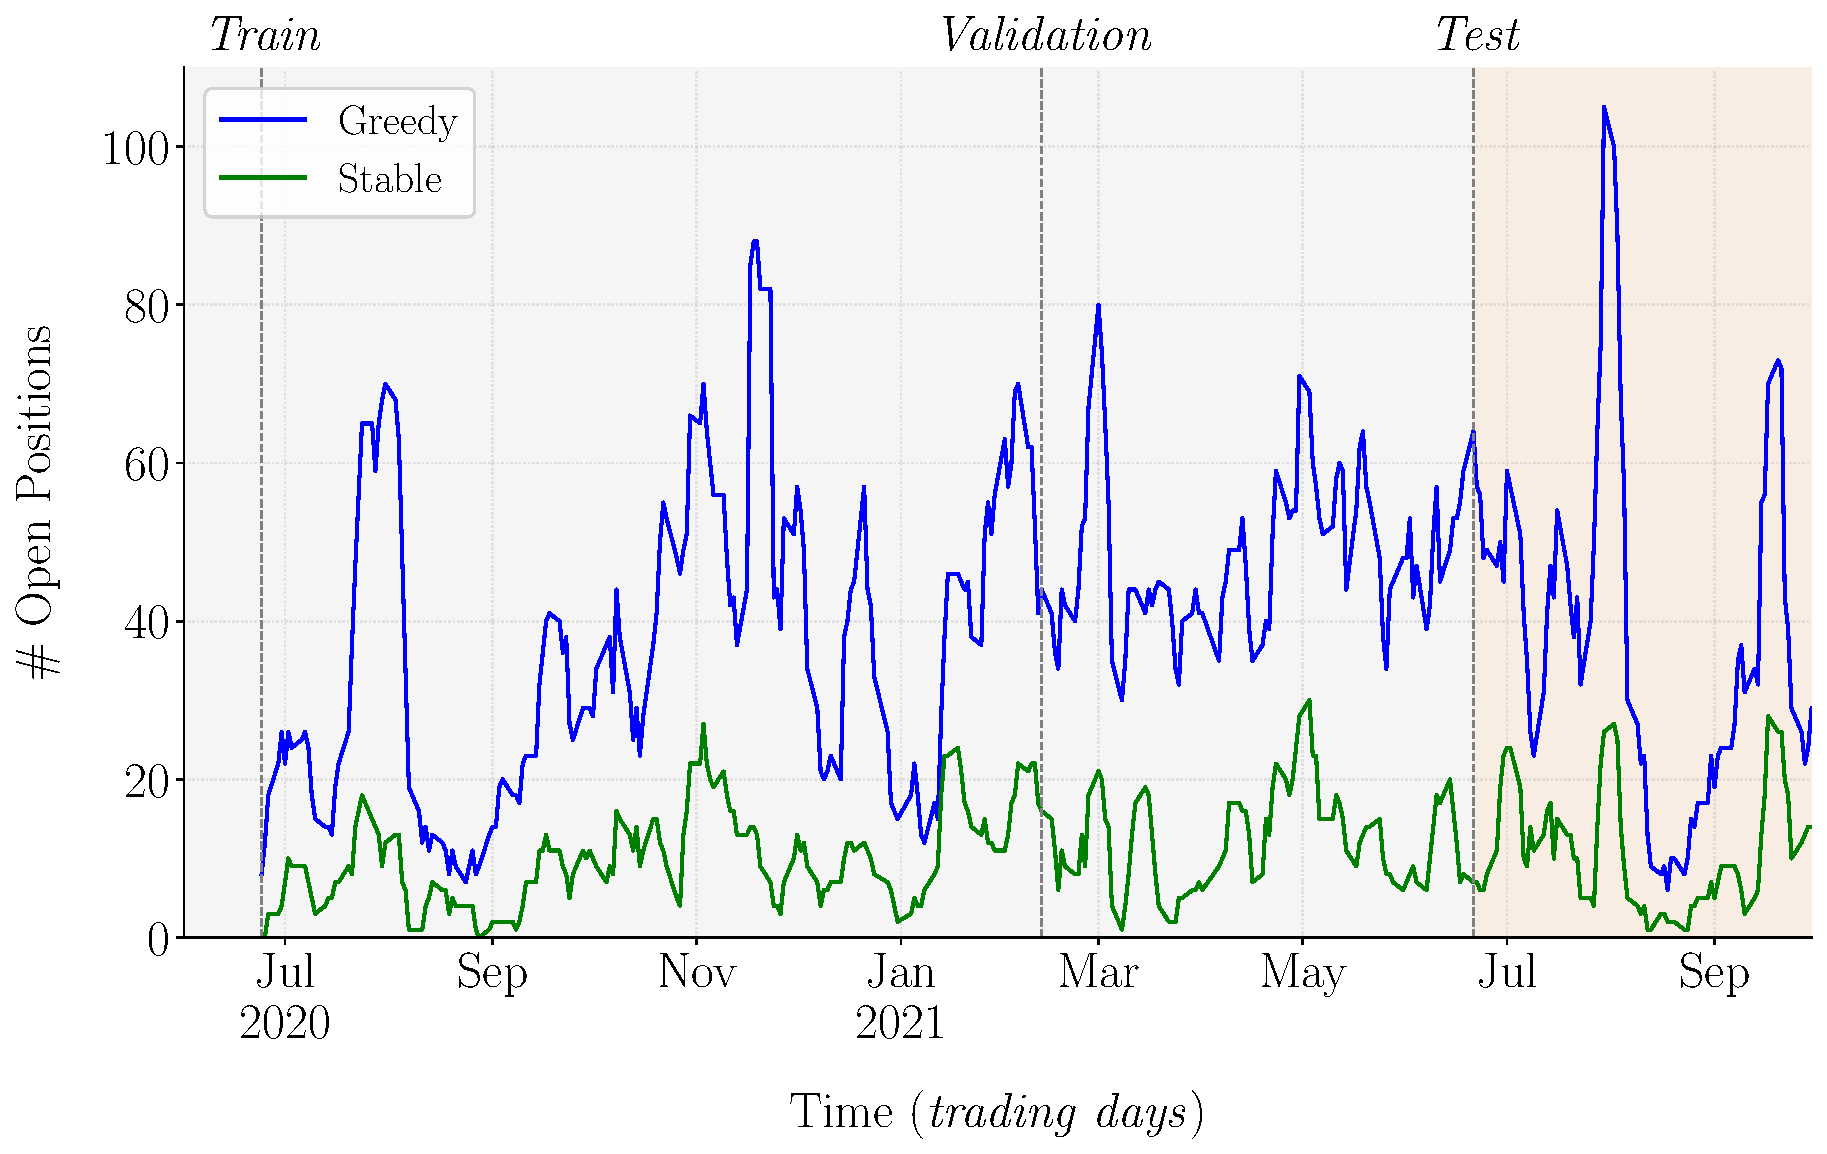
\includegraphics[scale=0.45]{fig_A6a_KMeans_Open_Positions.pdf}
\end{subfigure}

\vspace{0.7cm}

% Panel B: LLM
\begin{subfigure}{\textwidth}
\caption{Panel B: LLM Clustering}
\centering
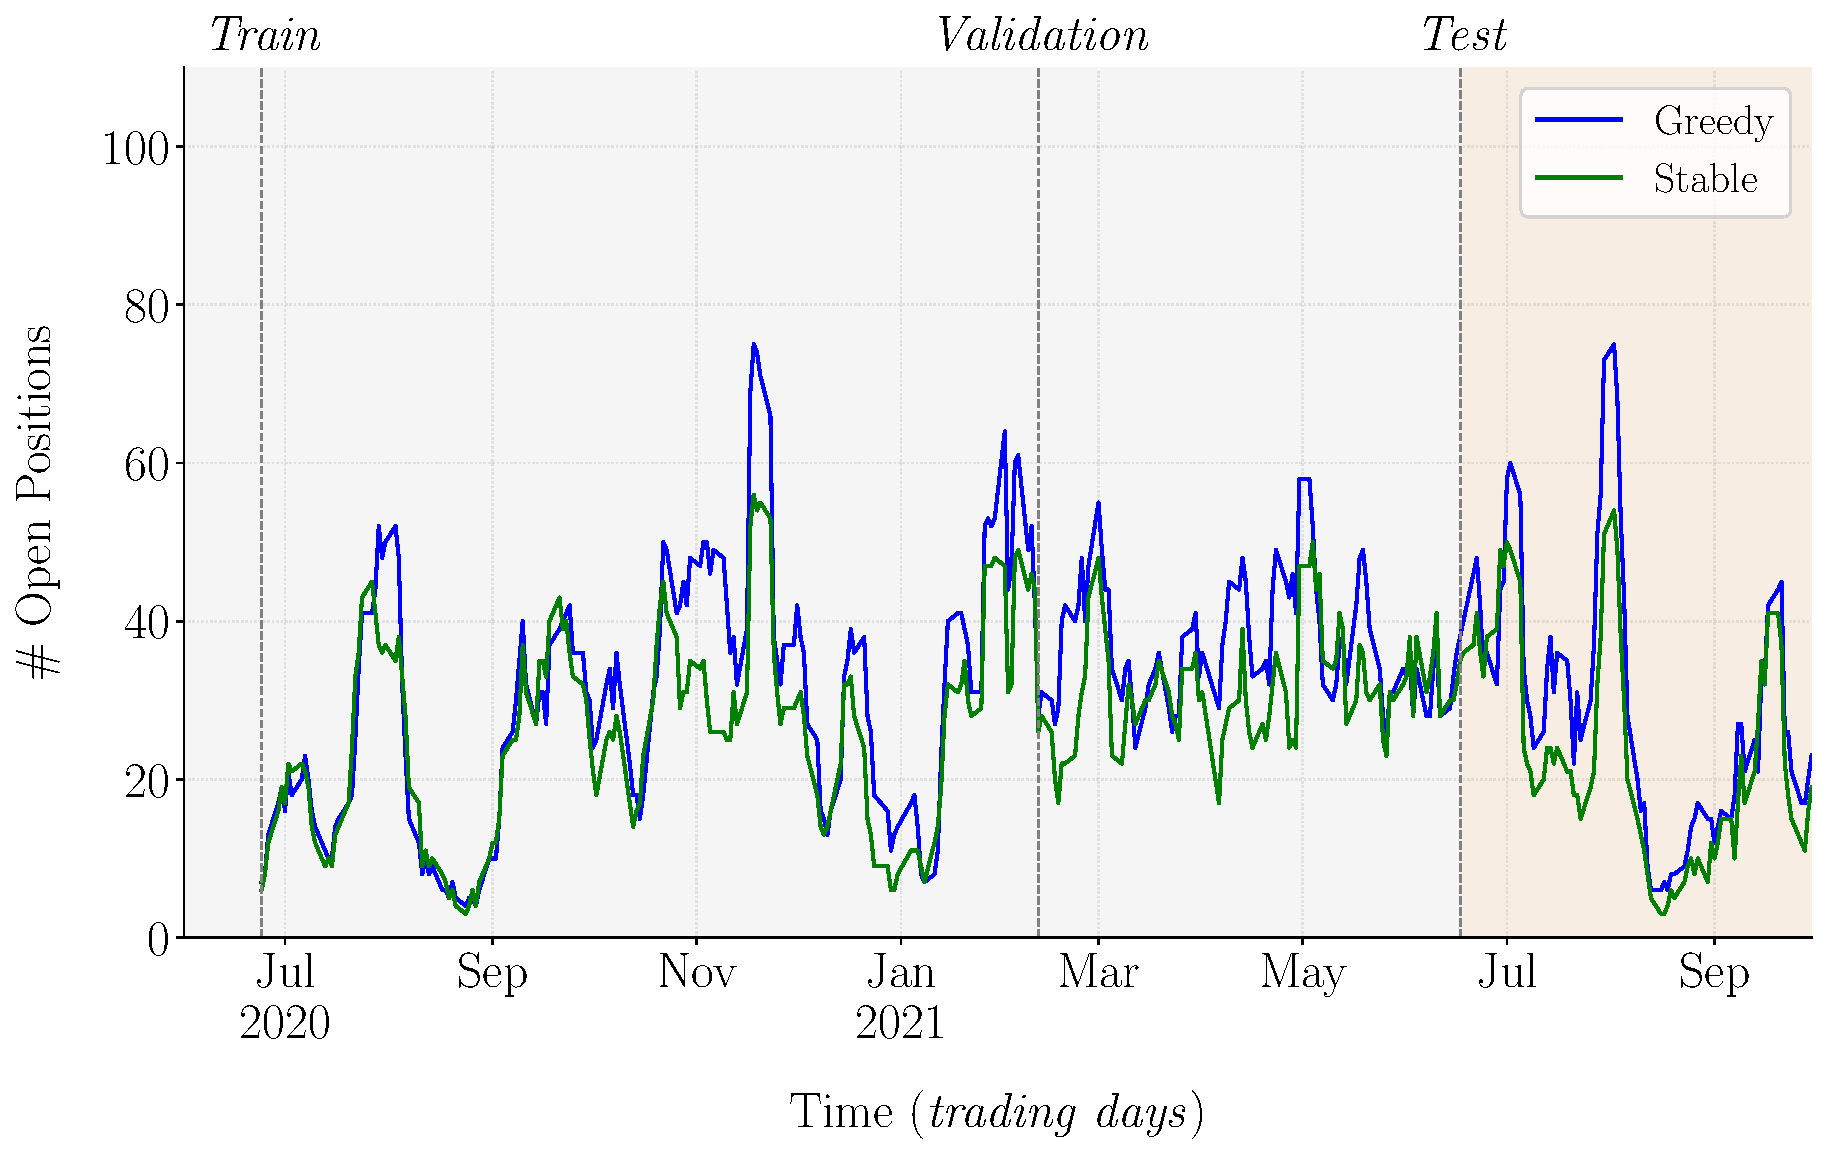
\includegraphics[scale=0.45]{fig_A6b_LLAMA_Open_Positions.pdf}
\end{subfigure}

\vspace{0.2cm}
\begin{minipage}{\textwidth}
\setlength{\parindent}{0pt}
{\footnotesize\textit{Note: 
This figure shows the daily evolution of the number of open positions for both Greedy (blue) and Stable (green) algorithms across different data splits (Train, Validation, Test) using KMeans clustering (Panel A) and LLM clustering (Panel B). The time period spans from July 2020 to September 2021. Vertical dashed lines separate the different data splits. The Greedy algorithm selects clusters that maximize (minimize) the cluster-average-$SR$ for long (short) positions, while the Stable algorithm minimizes the rank difference between training and validation rankings. The number of traded clusters is $\theta = 0.5k=13$ for KMeans ($k^*=26$ clusters) and $\theta = 0.5k=10$ for LLM ($k^*=20$ clusters).
}}
\end{minipage}
\end{figure}
%----------------------------------------------------

% < Reference to: \cref{fig:open_positions_comparison} >
The temporal evolution of open positions, as illustrated in \cref{fig:open_positions_comparison},  reveals fundamental differences in the stability and reliability of trading signals generated by KMeans versus LLM-based clustering approaches. The KMeans implementation exhibits pronounced volatility in position management, particularly evident in the Greedy algorithm's behavior, which shows extreme fluctuations ranging from 6 to 105 positions. This erratic pattern suggests that KMeans-detected clusters are highly sensitive to market noise and potentially capture transient correlations rather than fundamental relationships. The substantial divergence between Greedy and Stable algorithms under KMeans further underscores the method's instability, as even minor variations in cluster selection criteria lead to dramatically different trading decisions.
%
In stark contrast, the LLM-based approach demonstrates remarkably more coherent and stable position management. Both Greedy and Stable algorithms maintain more closely aligned position counts, typically ranging between 20 and 75 positions, with highly correlated temporal movements. This convergence in behavior between algorithms suggests that LLM-identified clusters capture more fundamental and persistent market relationships. Particularly telling is the test period performance, where KMeans exhibits increased position volatility and extreme spikes, while the LLM approach maintains consistent position patterns across both algorithms. This stability in the out-of-sample period provides strong evidence that LLM-derived signals, grounded in economic analysis of firm-specific shocks, generalize more effectively to unseen data.

%----------------------------------------------------
\inserthere{tab:trading_intensity_comparison}

\begin{table}[htbp] 
\caption{Trading Intensity Analysis: Model Comparison} 
\centering 
\label{tab:trading_intensity_comparison}

\begin{subtable}{\textwidth}
\caption{Panel A: KMeans}
\centering 
{\small
\begin{tabular}{lcccccccccc}
\toprule
\textbf{Split} & \textbf{Algorithm} & \multicolumn{4}{c}{\textbf{\# Open Positions}} & \multicolumn{2}{c}{\textbf{Trading Activity (\%)}} & \multicolumn{2}{c}{\textbf{Trading Costs (\%)}} \\
\cmidrule(lr{0.6em}){3-6} \cmidrule(lr{0.6em}){7-8} \cmidrule(lr{0.6em}){9-10}
& & \textbf{Avg}. & \textbf{Std}. & \textbf{Max} & \textbf{Min} & \textbf{Turnover} & \textbf{Changes/Pos.} & \textbf{Cost} & \textbf{Active} \\
\midrule
\multirow{2}{*}{All} & \textit{Greedy} & 40.1 & 18.59 & 105 & 6 & 32.03 & 0.798 & 0.0961 & 100.0 \\
 & \textit{Stable} & 10.77 & 6.41 & 30 & 0 & 34.75 & 3.228 & 0.1042 & 99.1 \\
\midrule
\multirow{2}{*}{Train} & \textit{Greedy} & 36.4 & 19.33 & 88 & 7 & 30.59 & 0.840 & 0.0918 & 100.0 \\
 & \textit{Stable} & 9.89 & 5.93 & 27 & 0 & 33.73 & 3.412 & 0.1012 & 98.2 \\
\midrule
\multirow{2}{*}{Validation} & \textit{Greedy} & 48.4 & 10.00 & 80 & 30 & 31.39 & 0.649 & 0.0942 & 100.0 \\
 & \textit{Stable} & 12.34 & 6.05 & 30 & 1 & 33.42 & 2.708 & 0.1003 & 100.0 \\
\midrule
\multirow{2}{*}{Test} & \textit{Greedy} & 38.8 & 21.74 & 105 & 6 & 35.86 & 0.925 & 0.1076 & 100.0 \\
 & \textit{Stable} & 10.84 & 7.47 & 28 & 1 & 39.30 & 3.626 & 0.1179 & 100.0 \\
\bottomrule
\end{tabular}
}
\end{subtable}

\vspace{0.6cm}

\begin{subtable}{\textwidth}
\caption{Panel B: LLM}
\centering
{\small
\begin{tabular}{lcccccccccc}
\toprule
\textbf{Split} & \textbf{Algorithm} & \multicolumn{4}{c}{\textbf{\# Open Positions}} & \multicolumn{2}{c}{\textbf{Trading Activity (\%)}} & \multicolumn{2}{c}{\textbf{Trading Costs (\%)}} \\
\cmidrule(lr{0.6em}){3-6} \cmidrule(lr{0.6em}){7-8} \cmidrule(lr{0.6em}){9-10}
& & \textbf{Avg}. & \textbf{Std}. & \textbf{Max} & \textbf{Min} & \textbf{Turnover} & \textbf{Changes/Pos.} & \textbf{Cost} & \textbf{Active} \\
\midrule
\multirow{2}{*}{All} & \textit{Greedy} & 31.8 & 14.84 & 75 & 4 & 39.21 & 1.234 & 0.1176 & 100.0 \\
 & \textit{Stable} & 26.61 & 12.16 & 56 & 3 & 39.18 & 1.473 & 0.1175 & 100.0 \\
\midrule
\multirow{2}{*}{Train} & \textit{Greedy} & 29.9 & 16.34 & 75 & 4 & 40.42 & 1.351 & 0.1212 & 100.0 \\
 & \textit{Stable} & 25.54 & 12.90 & 56 & 3 & 40.45 & 1.584 & 0.1213 & 100.0 \\
\midrule
\multirow{2}{*}{Validation} & \textit{Greedy} & 37.0 & 7.69 & 58 & 24 & 38.43 & 1.039 & 0.1153 & 100.0 \\
 & \textit{Stable} & 31.38 & 6.82 & 50 & 17 & 37.95 & 1.209 & 0.1138 & 100.0 \\
\midrule
\multirow{2}{*}{Test} & \textit{Greedy} & 29.7 & 16.24 & 75 & 6 & 37.56 & 1.264 & 0.1127 & 100.0 \\
 & \textit{Stable} & 23.43 & 13.71 & 54 & 3 & 37.85 & 1.615 & 0.1135 & 100.0 \\
\bottomrule
\end{tabular}
}
\end{subtable}

\vspace{0.5cm}
\begin{minipage}{\textwidth}
\setlength{\parindent}{0pt}
\small\textit{Note: 
This table presents trading intensity metrics for both Greedy and Stable algorithms across different data splits for two different models: KMeans (Panel A) and LLM (Panel B). 
The metrics are computed at a daily frequency. The `\# Open Positions' columns report position-related statistics: 
`Avg.' shows the mean number of concurrent open positions per day, `Std.' represents their standard deviation, while 
`Max' and `Min' indicate the maximum and minimum number of positions held simultaneously. Under `Trading Activity (\%)', 
`Turnover' is calculated as the sum of absolute changes in position sizes divided by the total portfolio size, expressed 
as a percentage; formally, $Turnover_t = 100 \times (\sum_i |w_{i,t} - w_{i,t-1}|)/(\sum_i |w_{i,t}|)$, where $w_{i,t}$ 
represents the position size in asset $i$ at time $t$. `Changes/Pos.' represents the average number of modifications per 
position per day, computed as the daily turnover divided by the average number of positions, providing insight into how 
actively individual positions are managed. 
The `Trading Costs (\%)' section reports `Cost' as the average daily implementation shortfall (computed as the product of daily turnover and a conservative transaction cost parameter of 30 basis points, representing both direct and indirect trading costs) expressed in percentage terms, while `Active' shows the percentage of trading days with at least one open position.
%
%The `Trading Costs (\%)' section reports `Cost' as the average daily implementation 
%shortfall (computed as the difference between gross and net returns) expressed in percentage terms, while `Active' shows 
%the percentage of trading days with at least one open position. 
All metrics are first computed daily and then averaged over their respective periods, except for Max and Min positions which represent the absolute extremes over each period.
}
\end{minipage}
\end{table}
%----------------------------------------------------

% < Reference to: \cref{tab:trading_intensity_comparison} >
The trading intensity metrics, detailed in \cref{tab:trading_intensity_comparison}, provide quantitative validation of the structural differences between KMeans and LLM clustering approaches. Under KMeans, the dramatic disparity between Greedy and Stable algorithms (averaging 40.1 versus 10.77 positions, with standard deviations of 18.59 and 6.41 respectively) reflects the method's fundamental instability. More concerning is the Stable algorithm's exceptionally high Changes/Position ratio (3.228 versus 0.798 for Greedy), indicating frequent position adjustments necessitated by the transient nature of KMeans-identified clusters.
The LLM implementation demonstrates substantially more balanced and stable metrics across both algorithms. Average position counts converge (31.8 for Greedy, 26.61 for Stable) with more moderate standard deviations (14.84 and 12.16), suggesting that both aggressive and conservative cluster selection approaches identify similar, fundamentally-driven trading opportunities. The more balanced Changes/Position ratios (1.234 and 1.473) and consistent turnover rates (approximately 39\% for both algorithms) indicate that LLM-identified clusters require less frequent rebalancing, supporting the hypothesis that they capture more persistent market relationships.
These patterns become particularly pronounced in the test period, where KMeans shows increased turnover (reaching 39.30\% for Stable) and position volatility, while the LLM approach maintains more stable trading activity (37.56\% and 37.85\% turnover for Greedy and Stable). This superior out-of-sample stability provides compelling evidence that LLM's economic approach to cluster identification produces more robust and generalizable trading signals compared to the purely statistical approach of KMeans.

%----------------------------------------------------
\inserthere{tab:portfolio_statistics_comparison_net}

\begin{table}[H] 
\caption{Portfolio Statistics Comparison: KMeans vs LLM Clustering (net of Trading Costs)} 
\centering
\label{tab:portfolio_statistics_comparison_net}

\renewcommand{\arraystretch}{1.1}
\newcolumntype{P}[1]{>{\centering\arraybackslash}p{#1}}

% Panel A: KMeans
\begin{subtable}{\textwidth}
\caption{Panel A: Statistics of $\mathcal{P}_{\text{KMeans}}$}
\centering
{\small
\begin{tabular}{
 P{1.28cm} P{0.9cm} P{0.9cm} P{0.9cm} P{0.9cm} P{0.9cm} P{0.9cm} 
 P{0.9cm} P{1cm} P{0.9cm} P{0.9cm} P{0.9cm} P{0.9cm}
}
\Xhline{2\arrayrulewidth}
\textbf{Split} & \textbf{Algo.} & \textbf{Cum. Ret.} & \textbf{Avg. Ret.} & \textbf{St. Dev.} & \textbf{Sharpe Ratio} & \textbf{Sortino Ratio} & \textbf{Max. DD} & \textbf{Calmar Ratio} & \textbf{Skew.} & \textbf{Exc. Kurt.} & \textbf{VaR 95\%} & \textbf{CVaR 95\%} \\
\Xhline{2\arrayrulewidth}
\multirow{2}{*}{All} & \textit{Greedy} & 0.780 & -17.3 & 9.6 & -2.0 & -1.7 & -24.7 & -0.7 & -0.48 & 3.90 & -14.0 & -24.2 \\
 & \textit{Stable} & 1.058 & 4.4 & 17.0 & 0.3 & 0.3 & -14.2 & 0.3 & 0.15 & 5.01 & -24.5 & -38.3 \\
\hline
\multirow{2}{*}{Train} & \textit{Greedy} & 0.823 & -25.6 & 11.6 & -2.5 & -2.0 & -18.2 & -1.4 & -0.51 & 2.71 & -19.4 & -29.9 \\
 & \textit{Stable} & 1.057 & 8.7 & 19.9 & 0.4 & 0.4 & -14.2 & 0.6 & -0.25 & 3.21 & -31.9 & -46.0 \\
\hline
\multirow{2}{*}{Validation} & \textit{Greedy} & 1.000 & -0.0 & 7.5 & -0.0 & -0.0 & -5.8 & -0.0 & -0.50 & 0.95 & -12.1 & -17.9 \\
 & \textit{Stable} & 1.050 & 14.7 & 13.4 & 1.0 & 1.0 & -5.3 & 2.8 & -0.27 & 1.99 & -20.6 & -30.9 \\
\hline
\multirow{2}{*}{Test} & \textit{Greedy} & 0.937 & -20.0 & 6.6 & -3.4 & -3.5 & -9.1 & -2.2 & 1.55 & 4.31 & -8.9 & -12.0 \\
 & \textit{Stable} & 0.924 & -23.6 & 14.2 & -1.9 & -2.0 & -10.0 & -2.4 & 2.48 & 14.59 & -20.6 & -28.5 \\
\Xhline{2\arrayrulewidth}
\end{tabular}
}
\end{subtable}

\vspace{0.5cm}

% Panel B: LLM
\begin{subtable}{\textwidth}
\caption{Panel B: Statistics of $\mathcal{P}_{\text{LLM}}$}
\centering
{\small
\begin{tabular}{
 P{1.28cm} P{0.9cm} P{0.9cm} P{0.9cm} P{0.9cm} P{0.9cm} P{0.9cm} 
 P{0.9cm} P{1cm} P{0.9cm} P{0.9cm} P{0.9cm} P{0.9cm}
}
\Xhline{2\arrayrulewidth}
\textbf{Split} & \textbf{Algo.} & \textbf{Cum. Ret.} & \textbf{Avg. Ret.} & \textbf{St. Dev.} & \textbf{Sharpe Ratio} & \textbf{Sortino Ratio} & \textbf{Max. DD} & \textbf{Calmar Ratio} & \textbf{Skew.} & \textbf{Exc. Kurt.} & \textbf{VaR 95\%} & \textbf{CVaR 95\%} \\
\Xhline{2\arrayrulewidth}
\multirow{2}{*}{All} & \textit{Greedy} & 0.891 & -8.5 & 9.7 & -0.9 & -1.0 & -12.3 & -0.7 & 1.44 & 9.81 & -15.7 & -21.2 \\
 & \textit{Stable} & 0.928 & -5.6 & 8.6 & -0.7 & -0.7 & -11.7 & -0.5 & 0.31 & 2.18 & -12.9 & -18.7 \\
\hline
\multirow{2}{*}{Train} & \textit{Greedy} & 0.910 & -13.4 & 11.5 & -1.2 & -1.3 & -12.3 & -1.1 & 1.63 & 8.83 & -19.4 & -23.2 \\
 & \textit{Stable} & 0.964 & -5.5 & 10.0 & -0.6 & -0.6 & -9.7 & -0.6 & 0.21 & 1.60 & -14.8 & -21.6 \\
\hline
\multirow{2}{*}{Validation} & \textit{Greedy} & 0.985 & -4.3 & 8.1 & -0.5 & -0.6 & -4.3 & -1.0 & 0.19 & 1.17 & -11.6 & -18.0 \\
 & \textit{Stable} & 0.947 & -14.3 & 7.0 & -2.2 & -2.0 & -6.1 & -2.4 & 0.17 & 1.17 & -13.0 & -16.5 \\
\hline
\multirow{2}{*}{Test} & \textit{Greedy} & 0.995 & -1.5 & 6.2 & -0.2 & -0.3 & -1.9 & -0.8 & 1.02 & 6.91 & -8.2 & -12.1 \\
 & \textit{Stable} & 1.009 & 3.1 & 7.0 & 0.4 & 0.5 & -1.8 & 1.7 & 0.91 & 1.98 & -10.8 & -12.4 \\
\Xhline{2\arrayrulewidth}
\end{tabular}
}
\end{subtable}

\vspace{0.5cm}
\begin{minipage}{\textwidth}
\setlength{\parindent}{0pt}
{\small\textit{Note:
Portfolio statistics of trading strategies based on clusters obtained from KMeans (Panel A) and LLM (Panel B) approaches.
The statistics provided include performance metrics (Cumulative Return, Average Return (\%)), risk measures (Standard Deviation (\%), Maximum Drawdown (\%), Value at Risk (\%), Conditional Value at Risk (\%)), risk-adjusted performance ratios (Sharpe Ratio, Sortino Ratio, Calmar Ratio), and return distribution characteristics (Skewness, Excess Kurtosis). These statistics are provided for both cluster-selection algorithms: Greedy and Stable.
Except for the Cumulative Return, all returns are annualized. The Sharpe Ratio is computed using the daily returns, assuming 252 trading days in a year. The Sortino Ratio is calculated using the daily downside returns. The Maximum Drawdown is the maximum loss from a peak to a trough. The Calmar Ratio is the ratio of the annualized return to the maximum drawdown. Skewness measures the asymmetry of the return distribution, while Kurtosis quantifies the tails' thickness. The Value at Risk (VaR) and Conditional Value at Risk (CVaR) are calculated at a 95\% confidence level.
%
All returns are calculated net of transaction costs. We implement a conservative transaction cost estimate of 30 basis points (0.30\%) per trade, which accounts for both direct costs (commissions, fees) and indirect costs (bid-ask spreads, market impact). 
%Transaction costs for each day are computed as the product of daily portfolio turnover and the transaction cost parameter ($TC = \text{turnover} \times 0.30\%$). Daily turnover is measured as the ratio of the absolute change in positions to the total portfolio size: $\text{Turnover} = \sum|Position_{t} - Position_{t-1}| / \sum|Position_{t}|$. This implementation follows standard practice in the literature (see, e.g., \citet{frazzini2012}) and provides a realistic assessment of strategy profitability in real market conditions.
%
The Greedy algorithm longs (shorts) clusters that maximize (minimize) the cluster-average-$SR$ in the validation sample subject to a positivity (negativity) constraint, while the Stable algorithm longs (shorts) clusters that minimize the rank difference between the training and validation rankings of the cluster-average-$SR$'s subject to a positivity (negativity) constraint, which is now imposed on both sample splits. In both algorithms, the cardinality of each leg is upper-bounded by a hyperparameter $\theta$.
The holding period of the beta-neutral positions is set to $L$ = 4 trading days for both approaches. The number of traded clusters is $\theta = 0.5k=13$ for KMeans ($k^*=26$ clusters) and $\theta = 0.5k=10$ for LLM ($k^*=20$ clusters). The selection criteria for these hyperparameters ($L,\theta$) is based on maximizing the Sharpe Ratios of the train and validation samples.
}}
\end{minipage}
\end{table}
%----------------------------------------------------
% < Reference to: tab:portfolio_statistics_comparison_net >
Finally, the introduction of trading costs significantly impacts the performance metrics of both clustering approaches (see \cref{tab:portfolio_statistics_comparison_net}), though with notably different implications for their practical viability. The KMeans-based strategy exhibits substantial performance degradation, particularly evident in the test period where both algorithms generate significant losses (Greedy: -20.0\%, Stable: -23.6\% average annual returns). This deterioration is accompanied by elevated risk metrics, with the Stable algorithm showing particularly concerning characteristics including high standard deviation (14.2\%) and extreme kurtosis (14.59) in the test period, suggesting frequent occurrence of extreme returns.
In contrast, the LLM-based approach demonstrates superior resilience to trading costs, maintaining more stable performance characteristics across all periods. Most notably, in the test period, the strategy achieves near-neutral to positive performance (Greedy: -1.5\%, Stable: +3.1\% annual returns) with substantially lower risk metrics (standard deviations of 6.2\% and 7.0\% respectively). The LLM approach's more moderate VaR and CVaR measures (around -8.2\% to -12.4\% in the test period) compared to KMeans (-8.9\% to -28.5\%) further underscore its superior risk management characteristics under transaction costs.
This stark contrast in net performance can be attributed to the fundamentally different nature of the signals generated by each approach. While KMeans' statistically-driven clusters require frequent rebalancing that amplifies transaction costs, the LLM's economically-motivated clusters appear to identify more persistent price patterns that remain profitable even after accounting for trading frictions. However, it is worth noting that neither approach was explicitly optimized for transaction cost efficiency, suggesting potential for further improvement through cost-aware portfolio construction. These results highlight that while our LLM-based news parser successfully captures predictable market reactions to news articles, practitioners implementing such strategies would benefit from incorporating transaction costs into their optimization framework.

%%%%%%%%%%%%%%%%%%%%%%%%%%%%%%%%%%%%%%%%%%%%%%%%%%%%%



%%%%%%%%%%%%%%%%%%%%%%%%%%%%%%%%%%%%%%%%%%%%%%%%%%%%%
\end{document}
